\documentclass[a4paper,9pt]{article}
\usepackage[utf8]{inputenc}
\usepackage{graphicx}
\usepackage{wrapfig}
\usepackage{gensymb}
\usepackage{amssymb}
\usepackage{multirow}
\usepackage[hidelinks, colorlinks=true, allcolors=black]{hyperref}
\usepackage{comment}
\usepackage{esvect}
\usepackage{float}
\usepackage{caption}
\usepackage[english]{babel}
\usepackage[margin=2cm,top=1cm,headheight=40pt,includehead]{geometry}
\usepackage{amsmath}
\usepackage{graphicx}
\usepackage{authblk}
\usepackage{svg}
\svgsetup{inkscapelatex=false}
\usepackage{lastpage}
\usepackage{multicol}
\usepackage{fancyhdr}
\usepackage{xcolor}
\usepackage{listings}
\usepackage{pdflscape}
\usepackage{subfig}
\usepackage[most]{tcolorbox}
\usepackage{subcaption}
\usepackage{float}
\captionsetup[subfigure]{labelformat = parens, labelsep = space, font = small}
\pagestyle{fancy}

\usepackage[sorting=none,backend=biber,
citestyle=authoryear, %% Hilfsprogramm "biber" (statt "biblatex" oder "bibtex")
%% Zitierstil (siehe Dokumentation)
natbib=true, %% Bereitstellen von natbib-kompatiblen Zitierkommandos
hyperref=true, %% hyperref-Paket verwenden, um Links zu erstellen
]{biblatex}
\addbibresource{References.bib}
\renewcommand{\familydefault}{\sfdefault}
\geometry{
 a4paper,
 right=17mm,
 left=20mm,
 top=10mm,
 bottom=25mm
 }


\definecolor{mGreen}{rgb}{0,0.6,0}
\definecolor{mGray}{rgb}{0.5,0.5,0.5}
\definecolor{mPurple}{rgb}{0.58,0,0.82}
\definecolor{backgroundColour}{rgb}{255,255,255}

\lstdefinestyle{CStyle}{
    backgroundcolor=\color{backgroundColour},   
    commentstyle=\color{mGreen},
    keywordstyle=\color{magenta},
    numberstyle=\tiny\color{mGray},
    stringstyle=\color{mPurple},
    basicstyle=\footnotesize,
    breakatwhitespace=false,         
    breaklines=true,                 
    captionpos=b,                    
    keepspaces=true,                 
    numbers=left,                    
    numbersep=5pt,                  
    showspaces=false,                
    showstringspaces=false,
    showtabs=false,                  
    tabsize=2,
    language=C
}

 \renewcommand{\thempfootnote}{\arabic{mpfootnote}}
 \captionsetup[table]{position=below} 
% \rhead{\includegraphics[width=6cm]{ETH_Zurich_header_1.jpg}}

\fancyhead{}
\fancyfoot{}
\fancyhead[R]{
\includegraphics[width=2.5cm]{ETH_logo_small_1.jpg}}
\fancyhead[L]{\textbf{\leftmark}}
\rfoot{\thepage}
\fancyfoot[L]{\textit{Semester Project}}
\setlength{\parindent}{0cm}
\newcommand{\emailaddress}{sognor@ethz.ch}
\begin{document}
\thispagestyle{empty}
\newgeometry{right=17mm,
 left=20mm,
 top=15mm,
 bottom=10mm}
\begin{center}


\begin{minipage}{\linewidth}
\begin{minipage}{0.20\linewidth}
   
\includegraphics[width=\linewidth]{Images/MIBS.png}\\[0.2cm]
\end{minipage}
\hfill
\begin{minipage}{0.25\linewidth}
     
\includegraphics[width=\linewidth]{Images/ETH.eps}\\[0.3cm]
\end{minipage}
\end{minipage}
\\[2cm]
\newcommand{\HRule}{\rule{\linewidth}{0.5mm}}
\textsc{\Huge Semester Project}\\[2cm]

\HRule \\[0.35cm]
\huge \texttt{Interactive Data Visualisation on a 3D-printed Sun Path Model}\\
\HRule \\[.4cm]


\begin{figure}[H]
    \centering
    \vspace{0cm}
    \includegraphics[height=12cm]{Images/Titlepagev2_1.jpg}
    \vspace{1cm}
\end{figure}
\end{center}
\begin{large}
\centering
\textrm{Rino Sogno}\\[0.3cm]
 \textrm{E-mail: \href{mailto:\emailaddress}{\emailaddress}}\\[1.5cm]
\begin{minipage}{\linewidth}
\begin{minipage}{0.3\linewidth}
\raggedright
   \textsc{ Zurich }
\end{minipage}
\hfill
\begin{minipage}{0.25\linewidth}
\raggedleft
  \textsc{\today}
\end{minipage}
\end{minipage}



\end{large}


\newpage
\restoregeometry
\thispagestyle{empty}

\vspace{1cm}
\noindent\hrulefill $\;\;\;\;${\Large \textbf{Contents}}$\;\;\;$ \noindent\hrulefill
\setcounter{tocdepth}{2}
\renewcommand*\contentsname{$\;$}
\large
\tableofcontents
\phantomsection
\normalsize
\vspace{3cm}
\noindent\hrulefill $\;\;\;\;${\Large \textbf{Acknowledgement}}$\;\;\;$\noindent\hrulefill \\
\\[1cm]
Thank you to the Chair of Architecture and Building systems, who hosted this semester project. Especially to my supervisor Christoph Waibel for his support and the good collaboration.\\
\\
A special appreciation to my friends, who  supported me in the last phase of the model assembly. Thank you very much for all the many hours spent on the very repetitive tasks of soldering, gluing, casing LEDs and sorting cables.

\newpage
\section{Introduction}
\begin{multicols}{2}
[
\subsection{Framework}
]
As part of the international Future Cities Laboratories (FCL) conference conducted in October 2023, the FCL research program hosted a public exhibition in the main hall of the ETH Zurich main building. The goal of the FCL is to help shaping sustainable cities and settlement systems through science, by design, in place, and over time.\\
\\
Within FCL, the "Powering the City" (POW) module, an international consortium of researchers from Singapore, Sweden, Switzerland, and the USA, were represented with an exhibition stand to showcase their ongoing research. The objective of the module is to investigate the deployment of building-integrated photovoltaic (BIPV) in urban environments, with themes revolving around it, such as socioeconomic, decentralized renewable energy, Vehicle-to-Grid, life cycle emissions, and architectural design.\\
\\
For this POW exhibition stand, we aimed to develop an interactive installation, involving electronic (and potentially mechanic) artefacts displaying the sun paths of Singapore and Zurich, as well as interactive data visualization techniques involving Augmented Reality (AR). The stand should combine information of the ongoing research, physical objects of BIPV panel prototypes, the interactive artefacts, as well as (touch-) screens to interact with the artefacts.
\end{multicols}

\begin{multicols}{2}
[
    \subsection{Targets and Milestones}
    ]
Within the aforementioned framework, this semester project was focused on the conceptualization, detailing and fabrication of the interactive artefact visualising the sun paths for the two studied locations (Zurich and Singapore).
The main goal was to decide upon the mode of visualisation (mechanical, light sources, etc.), the information visualisation control using an Arduino board, and to determine the design of the artefact as an art object. Once a final concept was derived, construction plans and details were produced and the artefact was manufactured
The following main milestones were recognised:
\end{multicols}
\begin{enumerate}
    \item Prototyping of the representation of the city scape (potentially 3D printed).
    \item Exploration of several technical options on how to visualize the sun path. This involves a static element showing the bounds of the sun paths (solstices) and some chosen sun paths, which could potentially be made from metal or wood. On the other hand, there is an interactive element (eg. using an LED-Mesh, using individual LEDS, using a mechanical element, a moving belt, or similar) to dynamically visualize the sun position or other information for different scenarios.
    \item This exploration was followed by a prototyping and ideation of the possible realizations of the most promising concepts on a small scale to prove its feasibility and visualization potential.
    \item This was combined with an exploration of the potential to show further information beyond the sun path (eg. PV penetration, grid emissions, temperature of the hour in a TMY, etc.) using the interactive representation of the sun. This involved programming a board (such as an Arduino) as a controller using the data given.
    \item Potentially creating a connection to an interface allowing the visitor to play (potentially involving “mini games”) or interact with the information shown and decide what he wants to see. This topic has an overlap with another ongoing semester project developing the AR setup and depends on the data given from the simulations.
    \item Once a final concept was derived, production plans and details were drawn. If needed, these were discussed with the respective ETH workshops or third party service providers, such that it was possible to produce the final product in time at its actual scale for the exhibition in October.
\end{enumerate}

\newpage
\section{Thoughts about the real sun path}
\begin{multicols}{2}
[
\subsection{The locations}
]
Both locations, Zurich and Singapore, lie on the northern hemisphere. Therefore, in both cases, the sun will come from the southern direction (cf. \textit{Figure} \ref{Map}). However, due to the close proximity of Singapore to the equator, the sun angle will be almost perpendicular to the ground. Thus, Singapore will show very little seasonal variation, as the sun angle does not change significantly over the seasons. In contrast, in Zurich, the sun angle is low and thus, seasonal variability is expected to be seen.
 \begin{figure}[H]
        \centering
        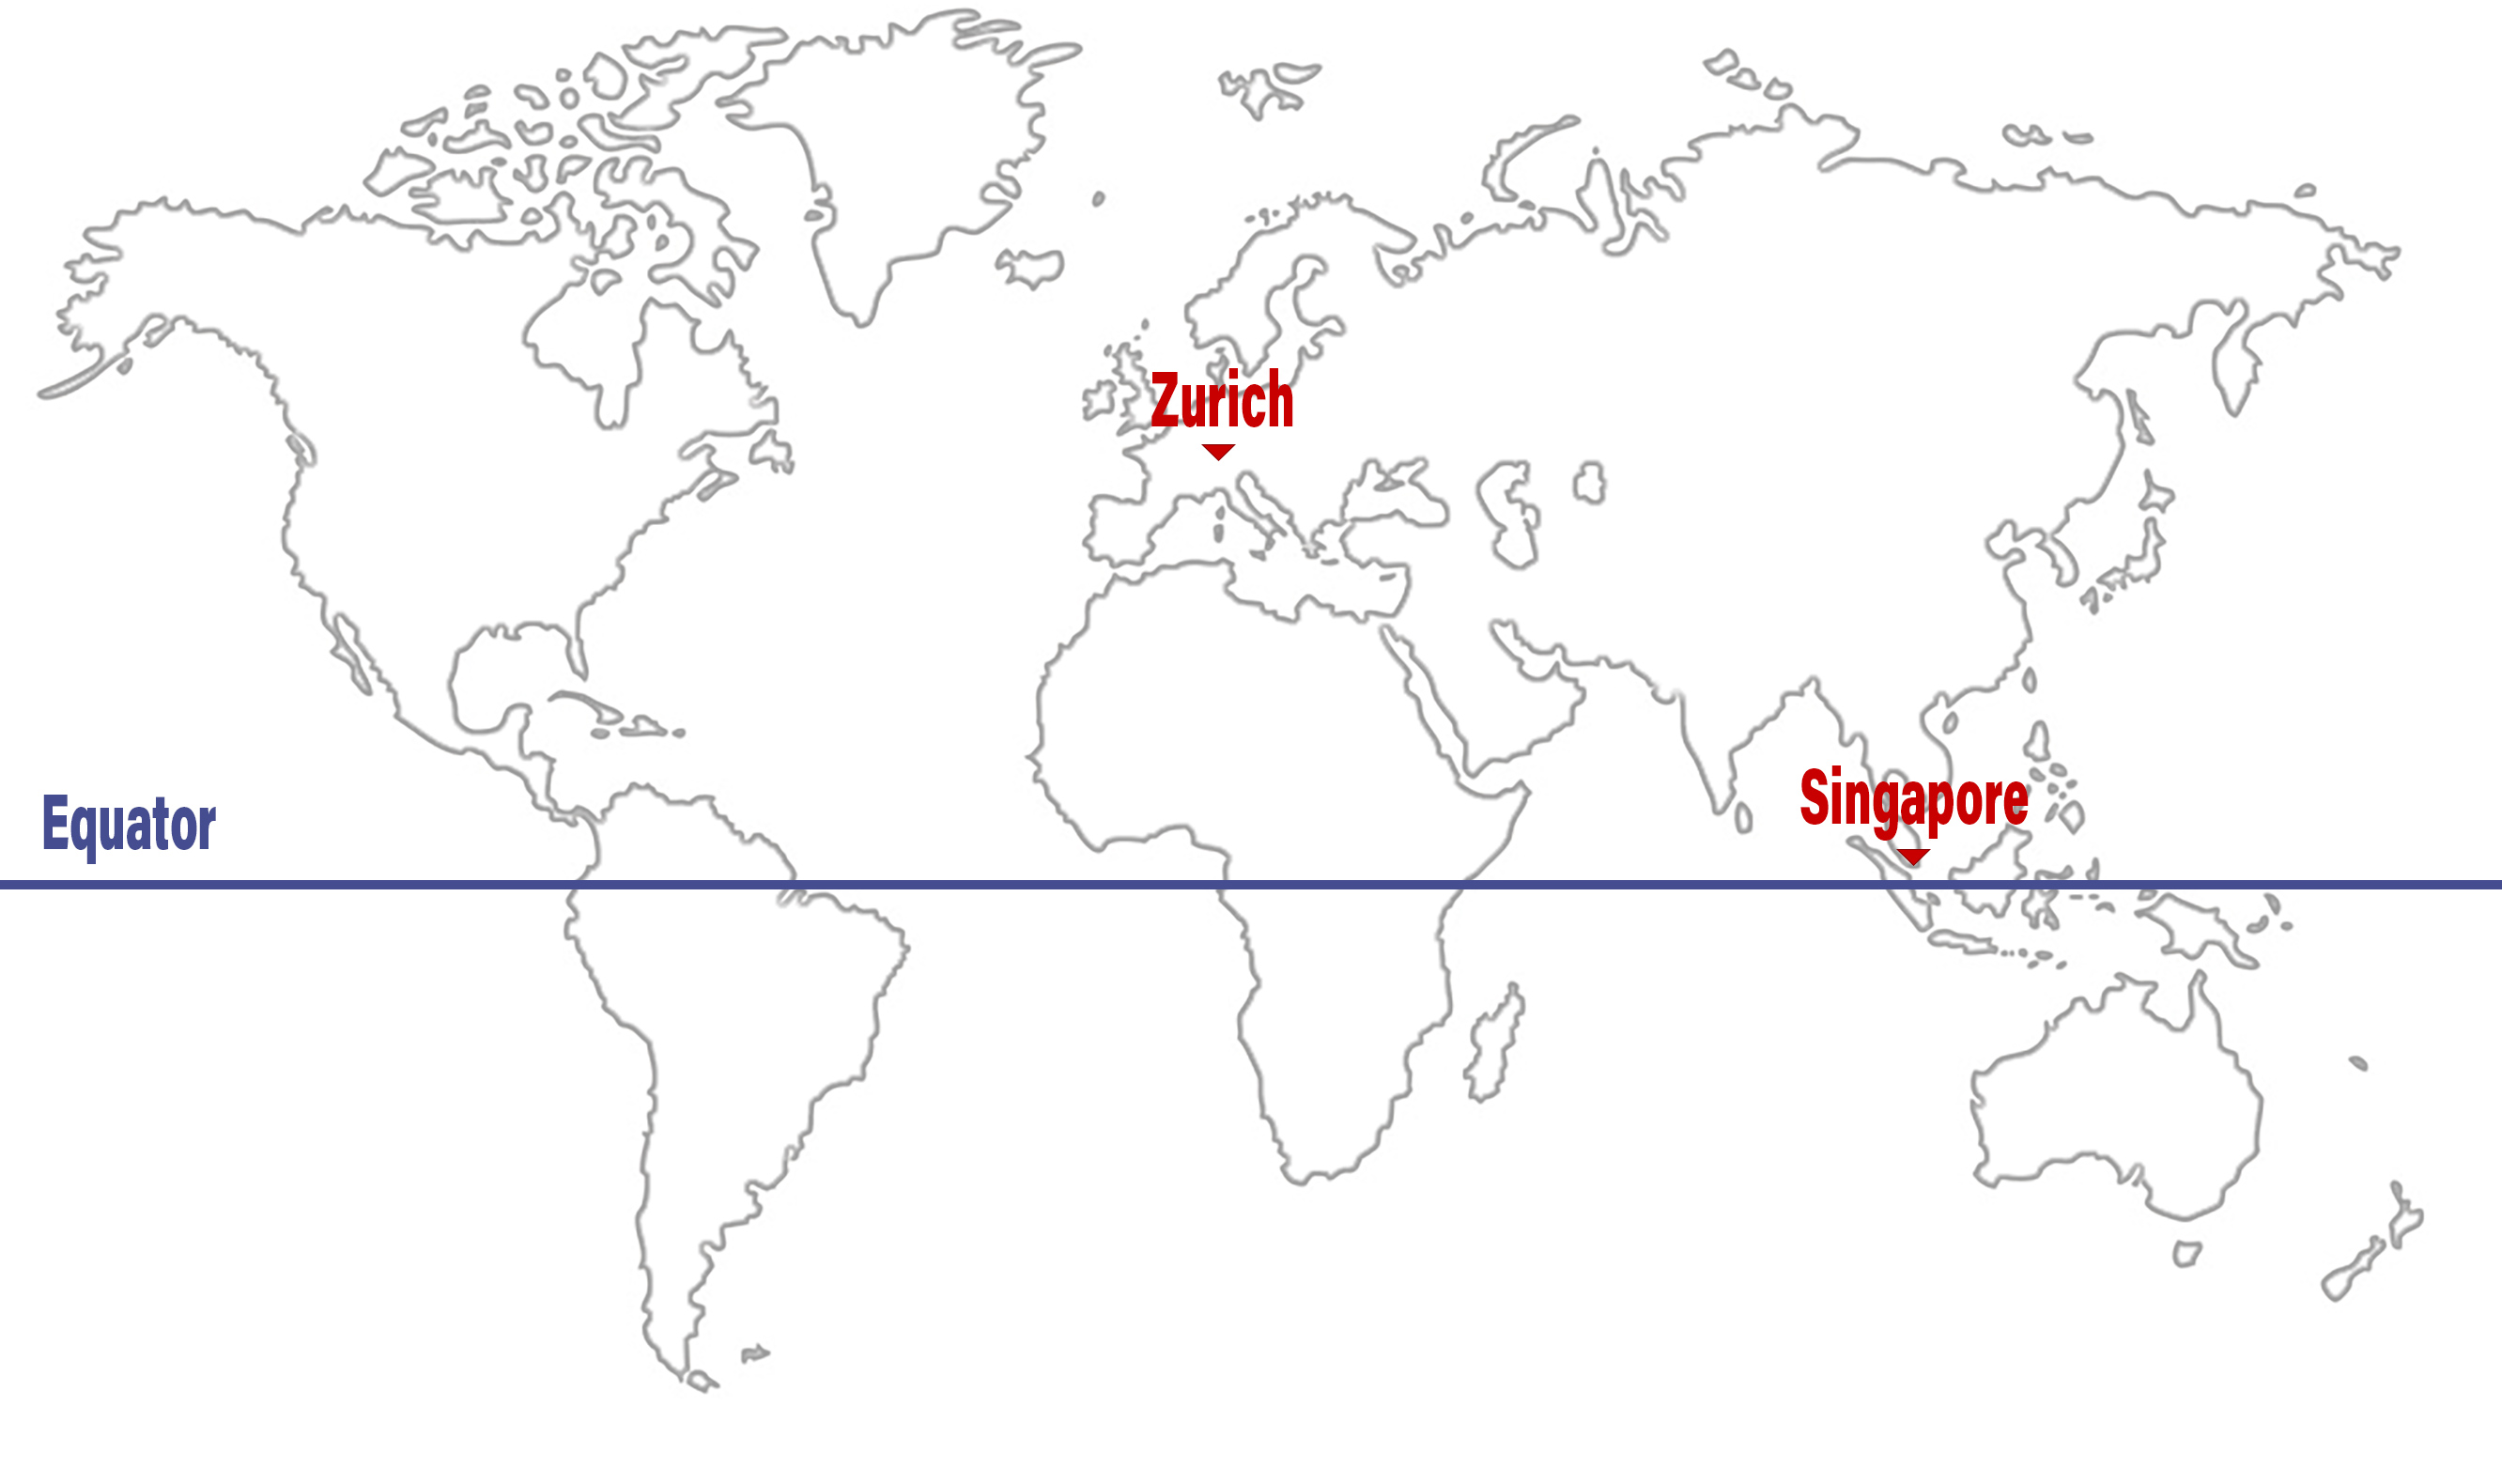
\includegraphics[width=1\linewidth]{Images/Worldmapp_1.jpg}
        \caption{The two studied Locations on the world map}
        \label{Map}
    \end{figure}
\end{multicols}
\begin{multicols}{2}
\subsection{The sun path in reality}

Taking a detailed look at the  sun paths for the two locations, one can see, that the possible sun positions lie in an area bounded by the horizon at the sunrise/sunset positions and the paths which the sun takes at the summer/winter solstice respectively. Every possible sun position must lie within this area.\\
\\
In general there are two interesting aspects to the movement of the sun. Over the course of a day the sun moves from the east to the west (for the northern hemisphere) on its daily path. However, the path is not the same for all days. Over the course of the year, the sun path moves. This movement goes from the longest path at the summer solstice to the shortest path at the winter solstice. In the middle of this movement, one can find the equinoxes (cf. \textit{Figure} \ref{sunpath}).\footcite{sunpath}
\columnbreak

\subsection{The analemmas}\label{anannn}

An often used concept in thinking about the sun's path are the analemmas. These are the shapes created by looking up onto the sky at the same hour every day of the year and marking the position of the sun. In doing so, one will realise, that the sun's positions at the same hour over one year moves along a shape looking similar to a figure eight (cf. \textit{Figure} \ref{sunpath2}). This shape is caused by the eccentricity of the earths orbit (different velocities at different positions) and the fact that the plane on which the earth rotates around the sun is tilted compared to the plane in which the earths rotation takes place (Eclptic). \footcite{analemma}

\end{multicols}

\begin{minipage}{0.28\linewidth}
    \centering
    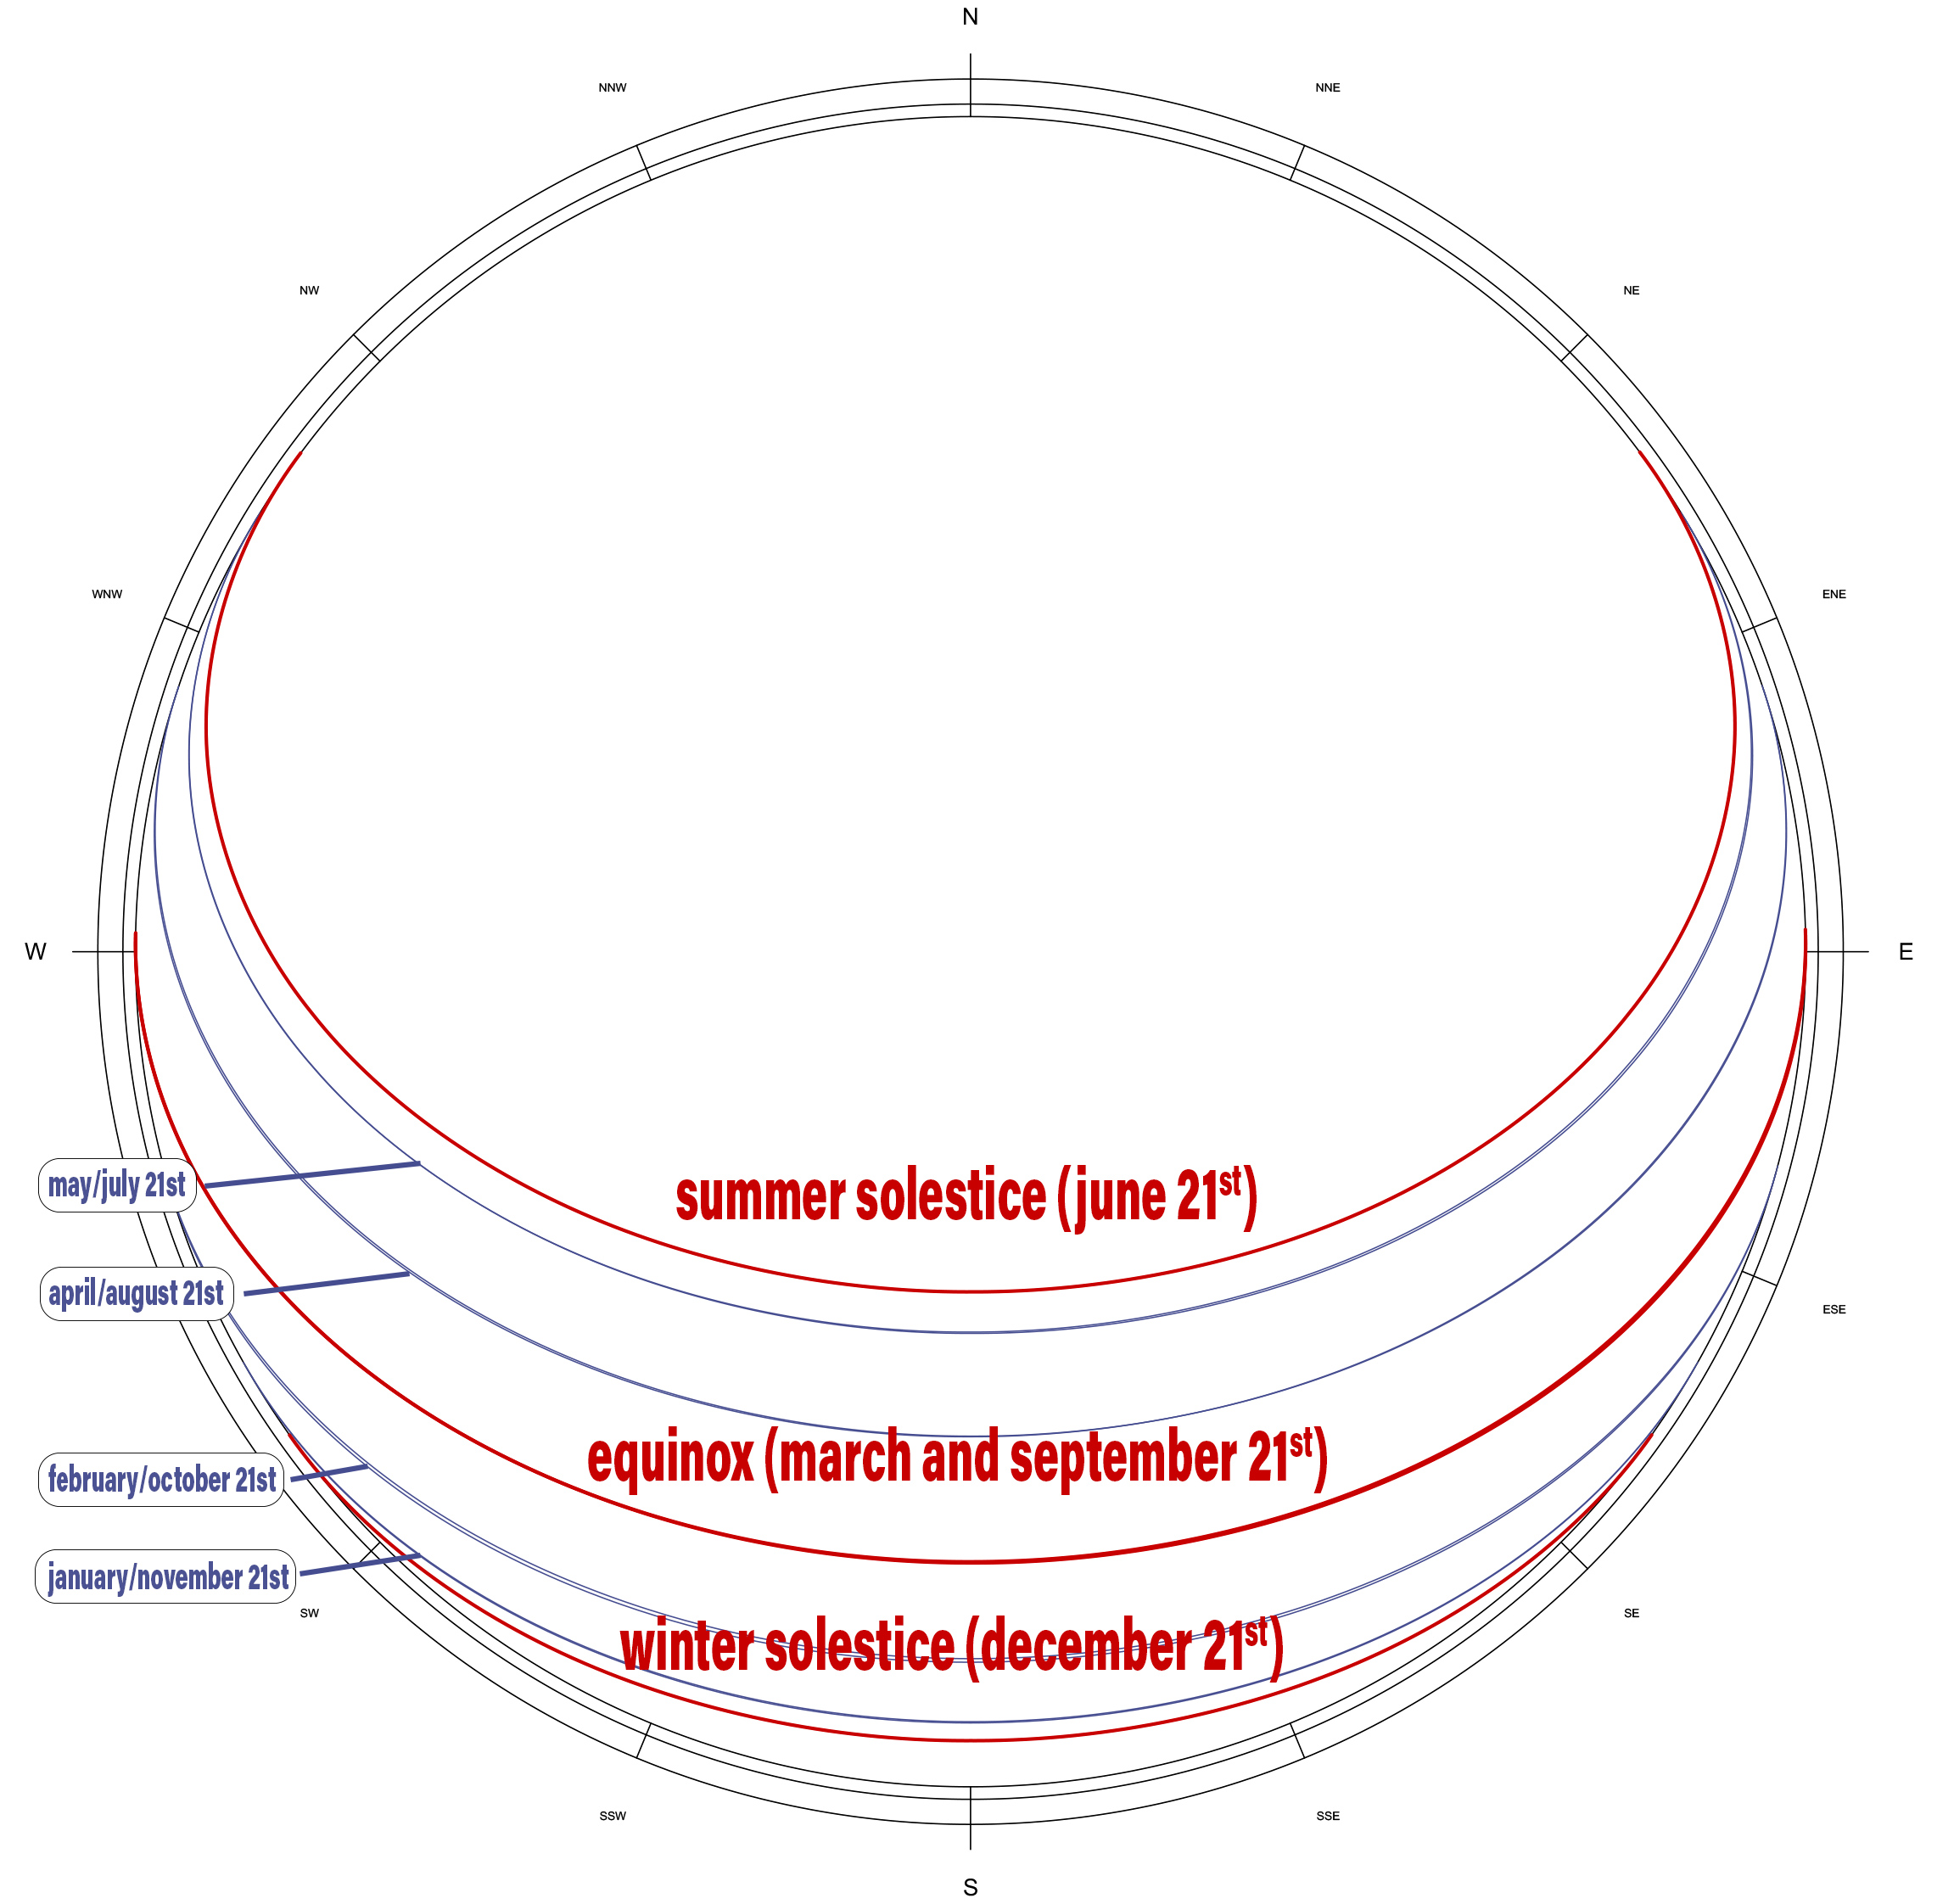
\includegraphics[width=\linewidth]{Images/sunpath_1.jpg}
  \\{Top view}
    \label{sunpath}
\end{minipage}
\hfill
\begin{minipage}{0.28\linewidth}
    \centering
    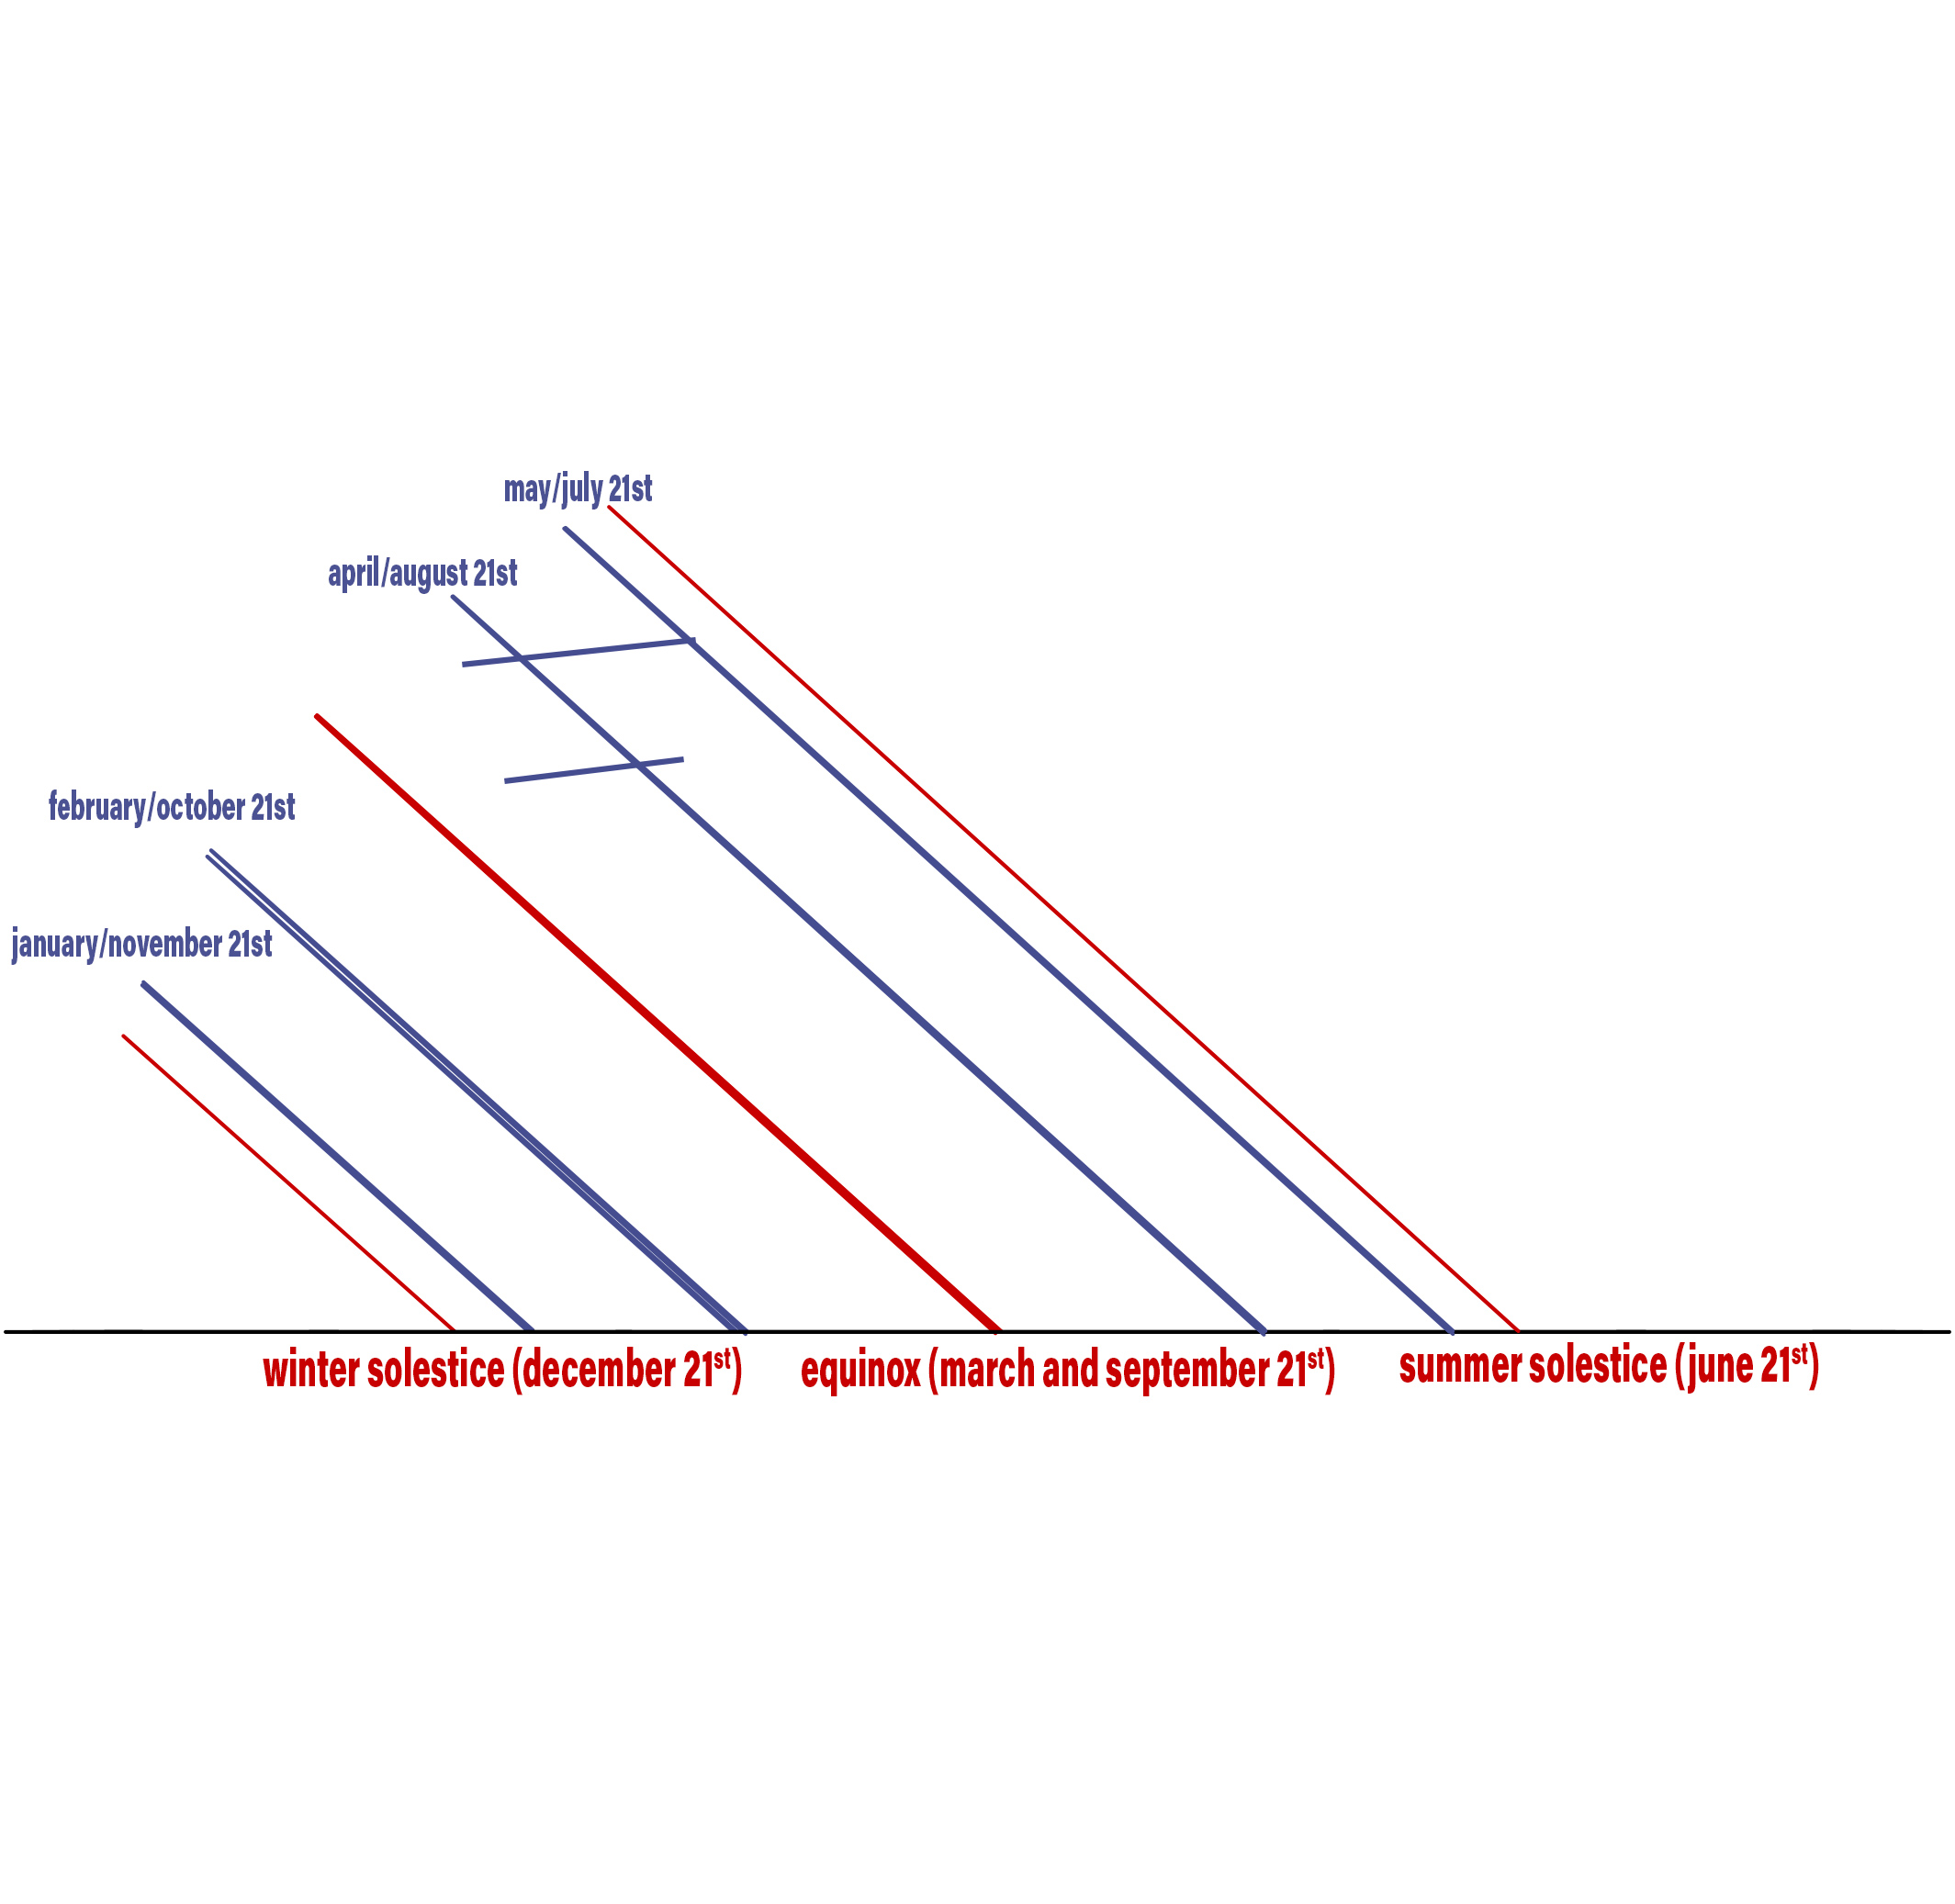
\includegraphics[width=\linewidth]{Images/sunpath2_1.jpg}
  \\{Side view}
     \label{sunpath1}
\end{minipage}
\hfill
\begin{minipage}{0.28\linewidth}
    \centering
    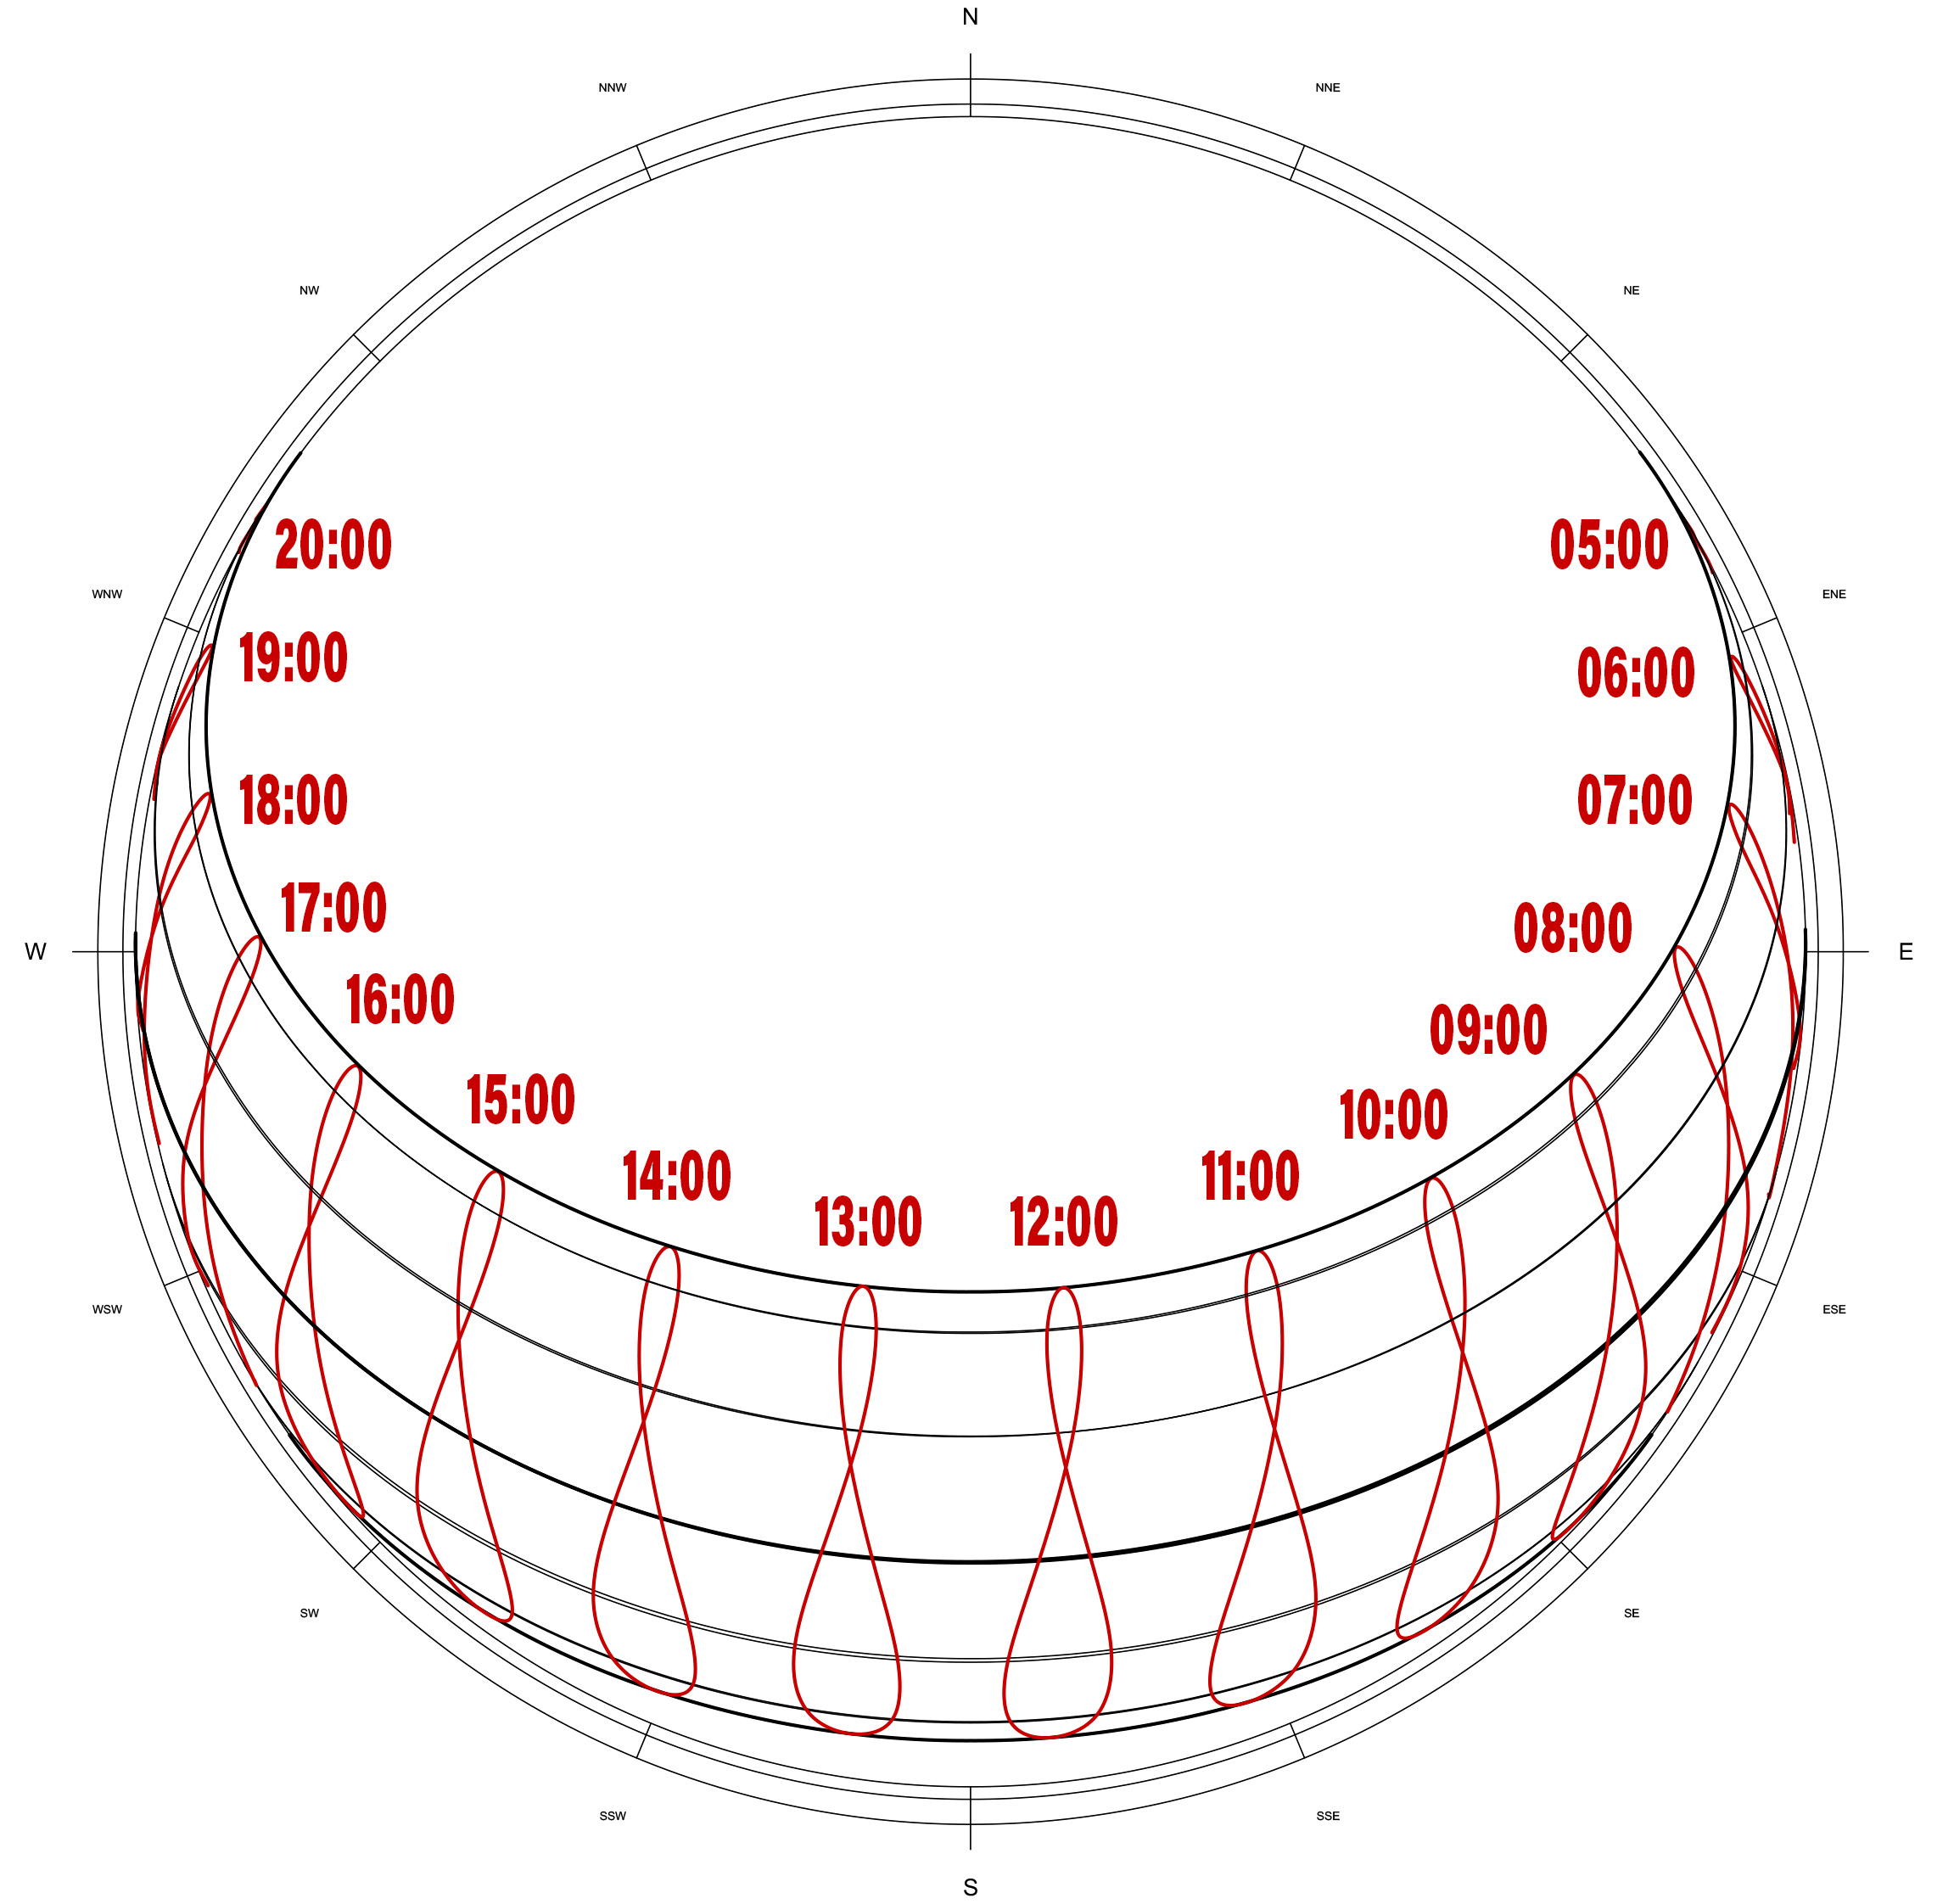
\includegraphics[width=\linewidth]{Images/sunpath3_1.jpg}
   \\{Analemmas}
     \label{sunpath2}
\end{minipage}
\captionof{figure}{Visualisation of the change of sun path over the seasons}
\newpage
\begin{multicols}{2}
[
\section{Conceptualizing the sun path in a visualisation}
]
Starting from the aforementioned explanation, there are two major ways to go in terms of interactive sun path visualisation: One possibility is to try to mimic the movement of the sun using actuators and move a light source in a continues movement across the sun path area. Lets call this the "mechanical approach" (cf. \textit{Figure} \ref{mechmus}). Another possibility is to choose a discrete set of positions on the sun path area (grid) and visualise this set as a mesh of individual light sources. Lets call this the "light approach". The use of LED lights is common in interactive exhibition setups (cf. \textit{Figure} \ref{lightmus}). In the following project both approaches where explored and the "light approach" was chosen for realisation in the end.
\end{multicols}

\begin{minipage}{0.48\linewidth}
        \centering
        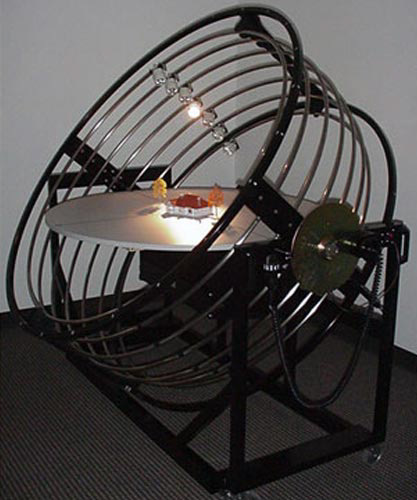
\includegraphics[width=.6\linewidth]{Images/heliodon_zoom.jpg}
      \\{HPD Model 126 Heliodon \footnotemark }
      

    \end{minipage}
    \footnotetext{\footcite{epfl}}
    \hfill
    \begin{minipage}{0.48\linewidth}

        \centering
        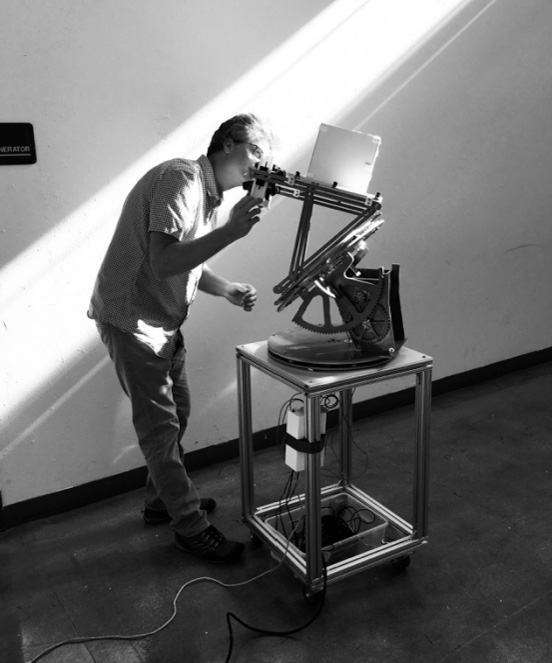
\includegraphics[width=.6\linewidth]{Images/Screenshot 2023-10-19 185345-2.jpg}
        \\{Heliodon for daylight analysis \footnotemark}
        
\end{minipage}
\footnotetext{\footcite{helo}}
\captionof{figure}{Different mechanical setups used in the visualisation and exploration of the sun path}
\label{mechmus}


\begin{multicols}{2}
The dimensions of the sun's path are a many fold bigger than we humans are. As a result, we are always looking up to the sun or the sun path and the sun shines down on us. However, looking at the planned exhibition model, the models dimension is way below our human scale. Meaning the perspective shifts from a looking up to the sun to a looking down at the sun path model and the model of the city. We are no longer immersed into the cityscape and the sun system, but suddenly in a floating outside position.\\
This means for the visualisation, that the light source(s) mimicking the sun not only need to shine onto the model of the city (the usual perception of the sun shining down onto the earth), but also needs to shine away from the model towards us, the viewer, such that we can localise the position of the sun looking from above.
\end{multicols}
\begin{minipage}{0.48\linewidth}
        \centering
        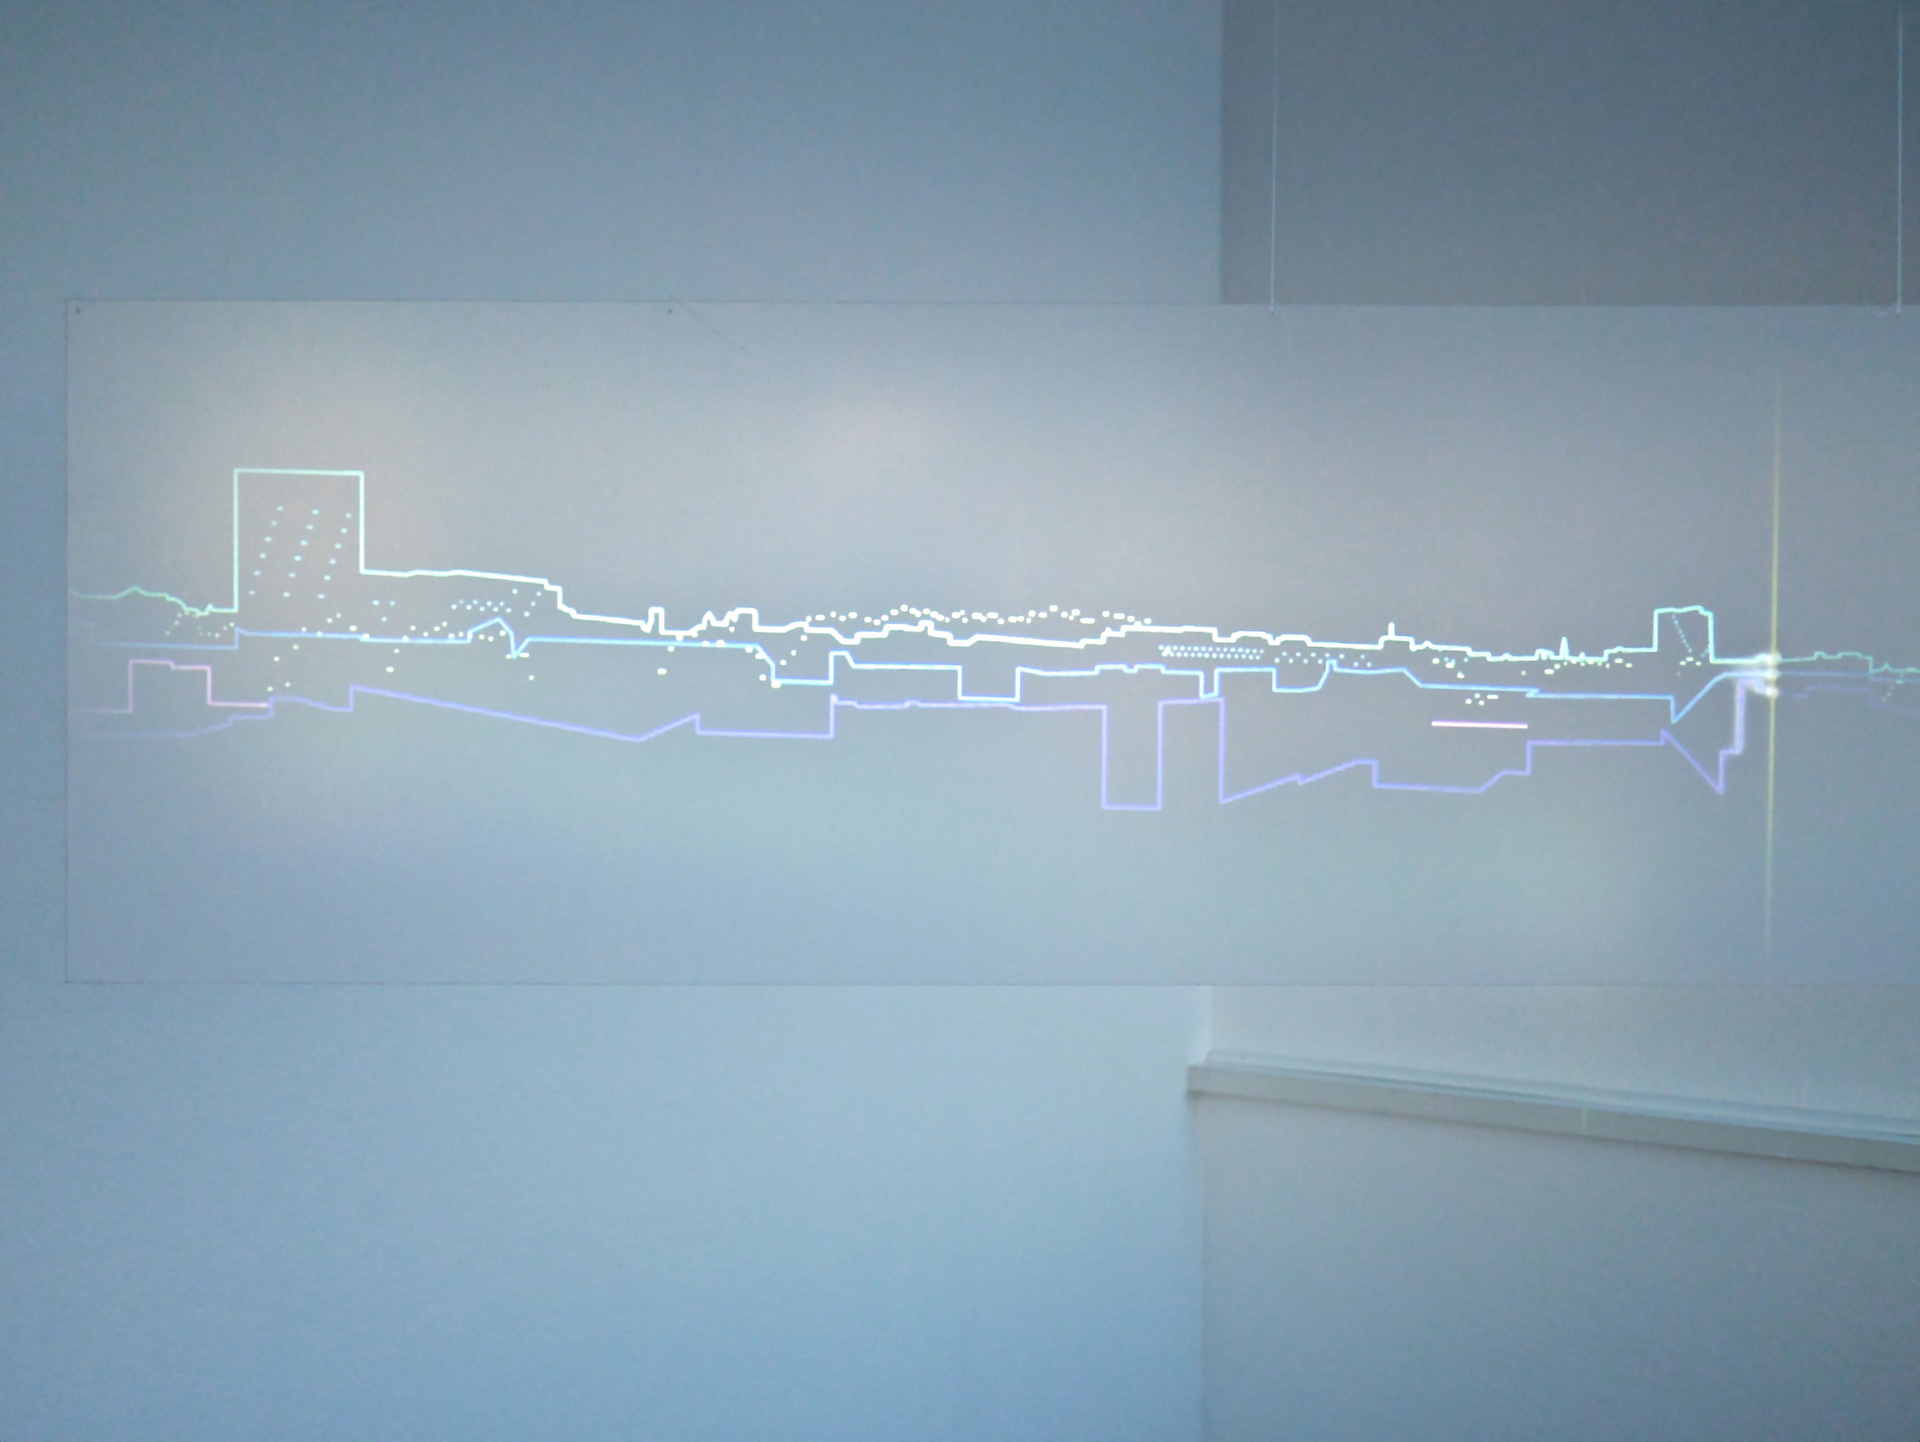
\includegraphics[width=.9\linewidth]{Images/sensing30.jpg}
      \\{Sensing the City - interactive sensor data visualisation \footnotemark }
    

    \end{minipage}
    \footnotetext{\footcite{snes}}
    \hfill
    \begin{minipage}{0.48\linewidth}

        \centering
        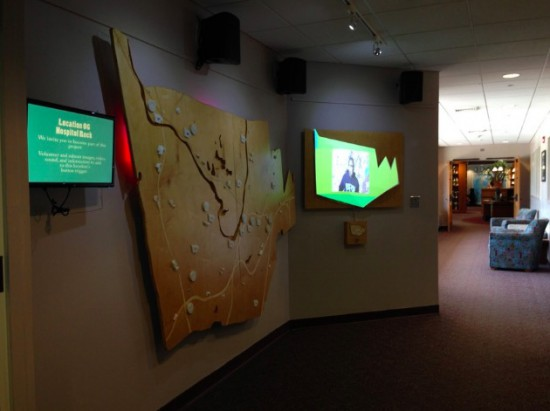
\includegraphics[width=.9\linewidth]{Images/MapProject-e1473975181395.jpg}
        \\{community-made, interactive town map \footnotemark}
        \label{protohoriz}
\end{minipage}
\footnotetext{\footcite{map}}
\captionof{figure}{Visual exhibition setups using lights do display information}
\label{lightmus}
\newpage
\begin{multicols}{2}
[
\section{Prototyping of different approaches}
]
Based on the aforementioned thoughts there are two directions to explore. A moving mechanic or a grid of lights.
\subsection{The mechanical approach}
Looking at the area in which the sun moves over the course of the year, it can be seen, that we are dealing with at least two dimensional movements. Thus, our mechanical system will need at least two actuators. Thinking of this surface as a two dimensional space, one can choose the base vectors (and thus, the two directions the actuators act in) in a variety of ways. However, there are two choices of coordinate system, where the directions potentially have an intuitive meaning to the viewer. These approaches are described and explored below.
\subsubsection{Horizontal Coordinate System Model }
    \label{hor}
    The horizontal coordinate system is often used to describe the position of a star (eg. the sun). To do so, the position is split into an Azimuth and an Altitude Angle. Therefore, using this model to create a mechanic to move a light source simulating the sun, means having a rotational movement and a movement along a bow in vertical direction (cf. \textit{Figure} \ref{horizontalcoord})
     
   
    A prototype was built exploring the possibilities which such a mechanic setup has. This setup would need two stepper motors and a turn table around the model carrying a bowed rod, along which the light source (sun) can move up and down (cf. \textit{Figure} \ref{protohoriz}). The downside of this coordinate system is, that to trace the path the sun takes over a day, a simultaneous movement of both motors would be necessary, which makes the programming of the movement complex. Furthermore this choice of coordinate system has a disadvantage in its appearance, as the visitor sees the two axes, but not the trace of the actual sun path. From an educational standpoint it would be more interesting to make the sun path visible for the viewer. To do so, an additional installation (eg. metal wire mesh) would be needed.
    
    \end{multicols}
    
      \begin{minipage}{0.48\linewidth}
         \begin{figure}[H]
        \centering
        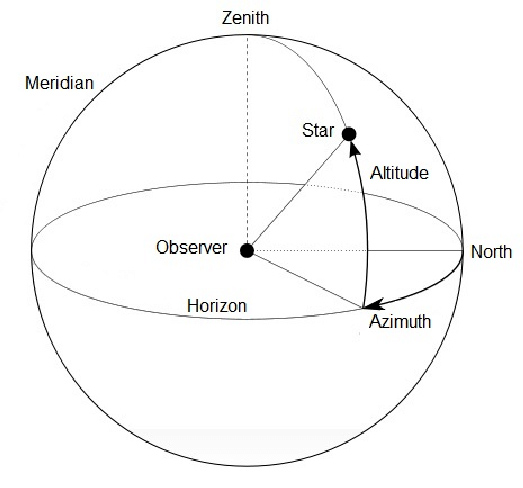
\includegraphics[width=.6\linewidth]{Images/horizontal coord_1.jpg}
        \captionof{figure}{The horizontal coordinate system \footnotemark }
        \label{horizontalcoord}
    \end{figure}
    \end{minipage}
    \hfill
    \begin{minipage}{0.48\linewidth}
         \begin{figure}[H]
        \centering
        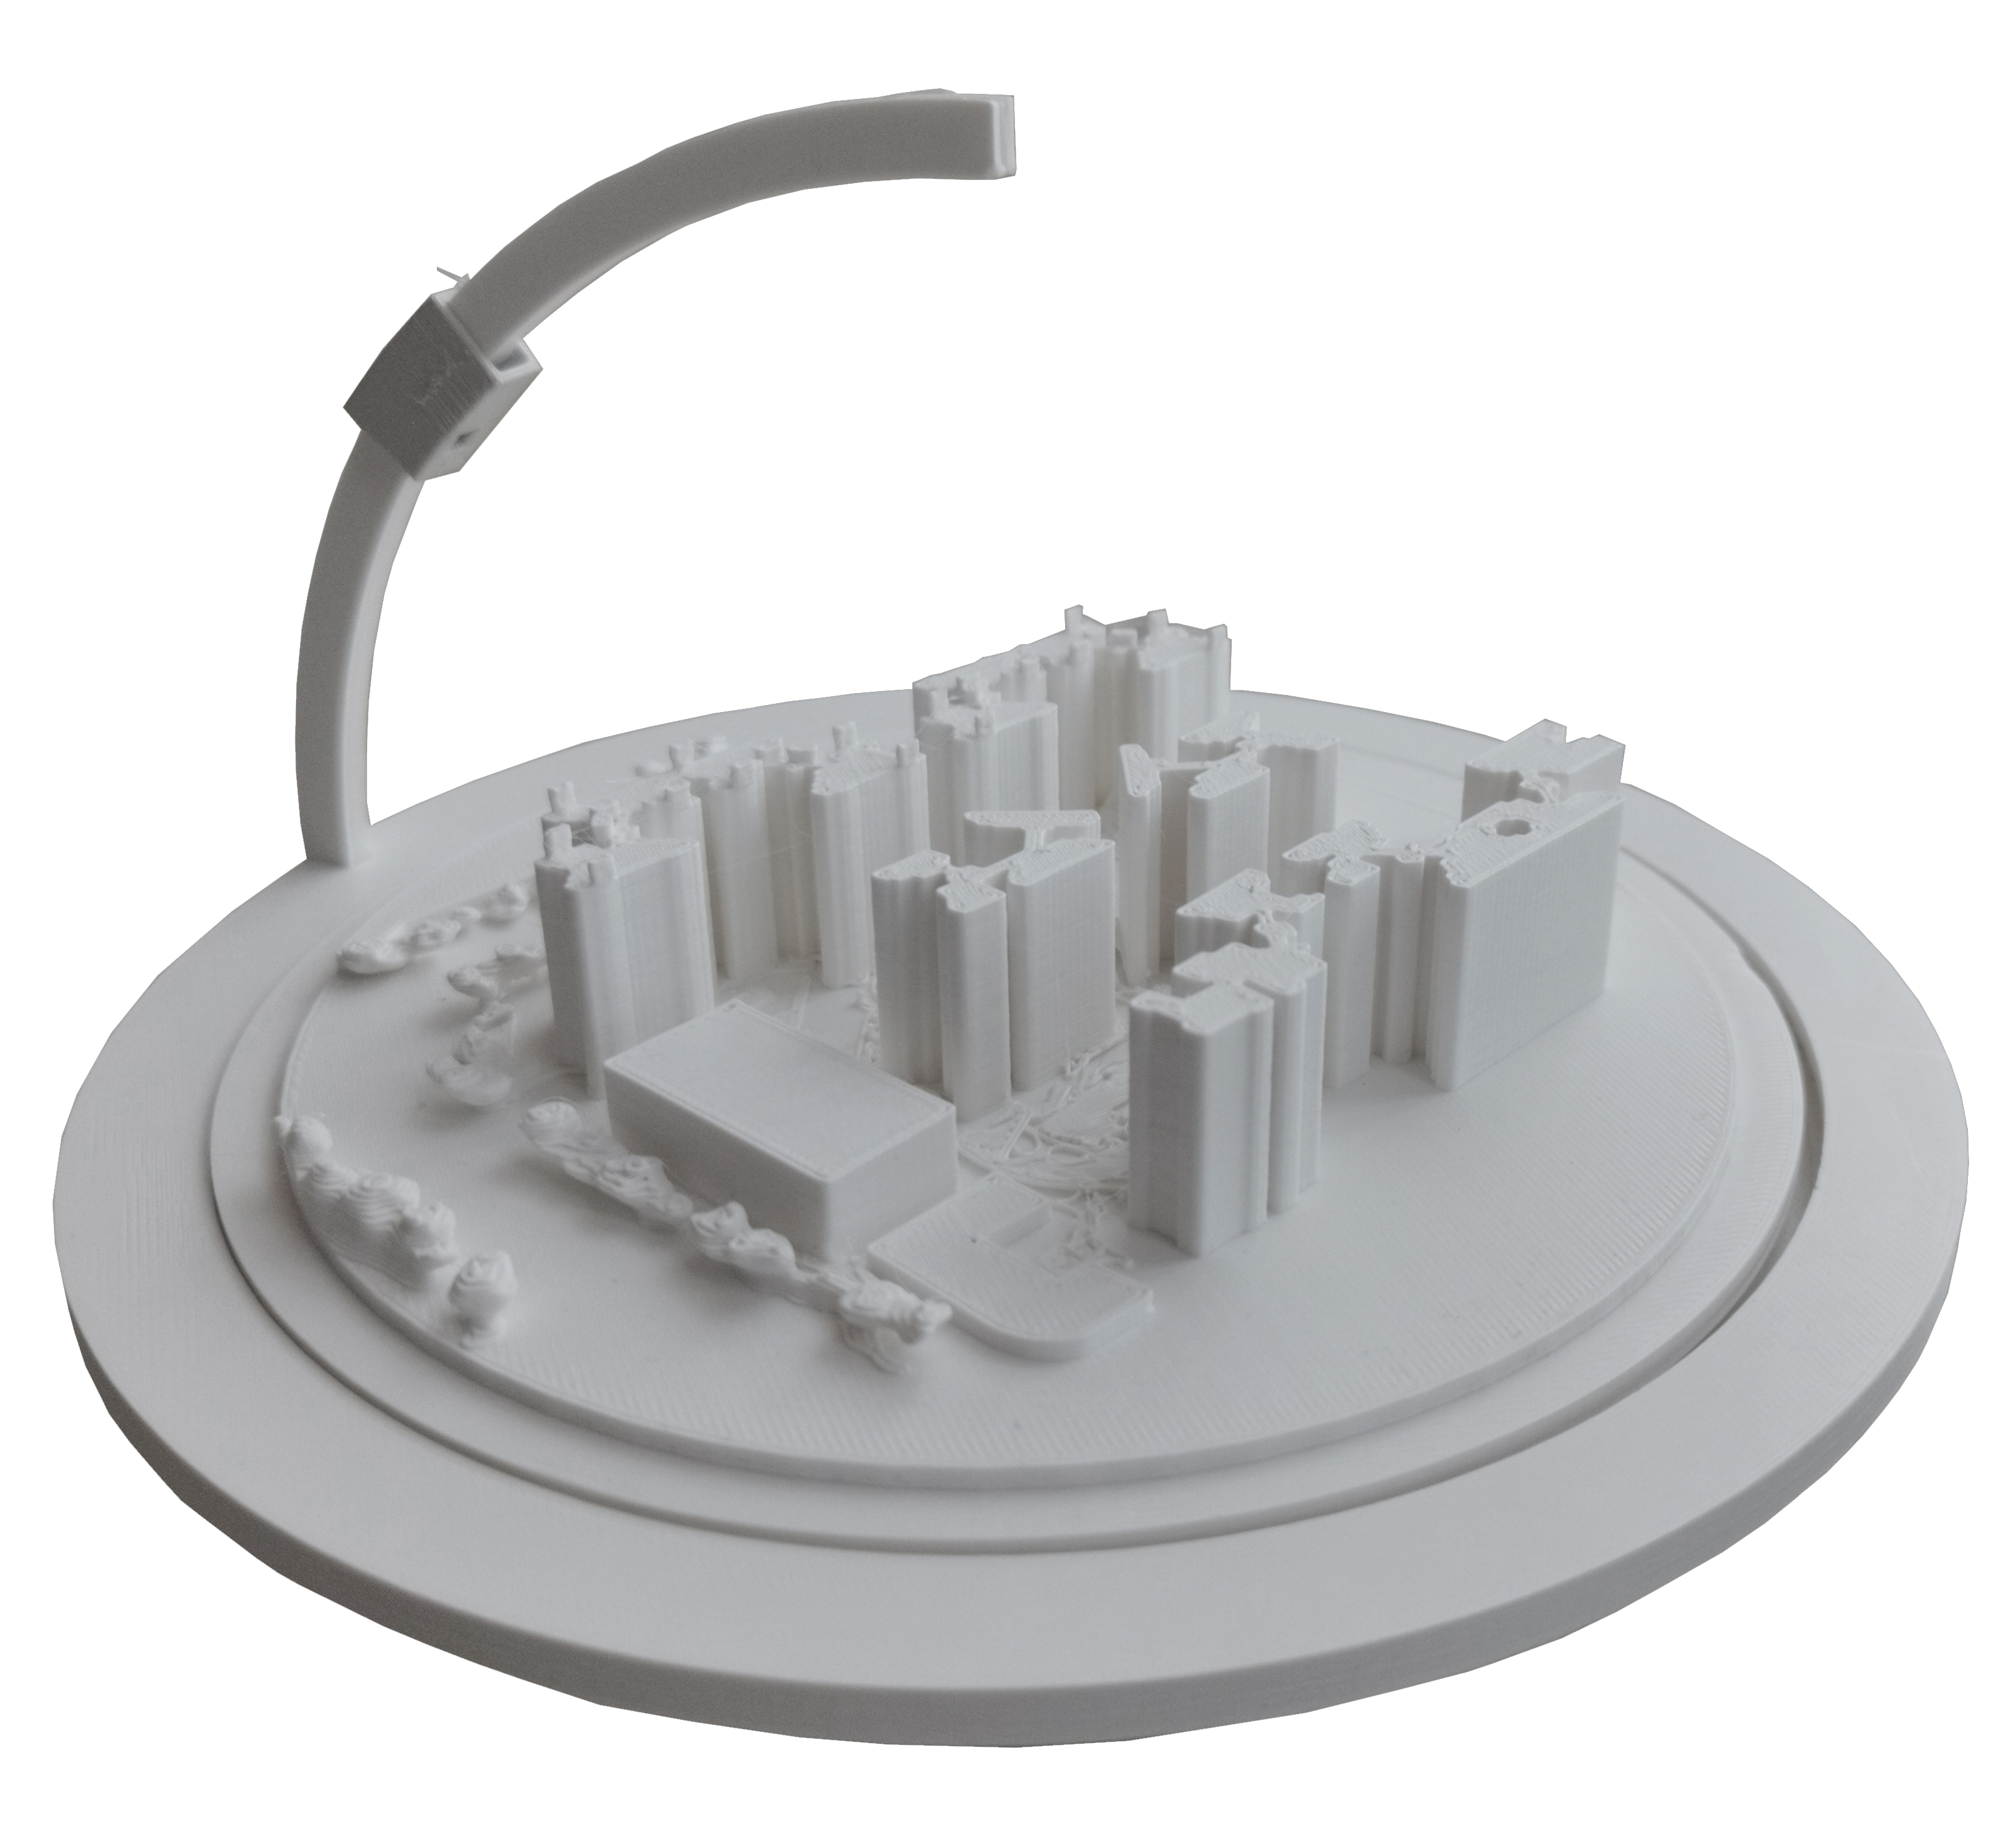
\includegraphics[width=.6\linewidth]{Images/prototyp hor2_1.png}
        \captionof{figure}{Fully functional prototype using a horizontal coordinate system}
        \label{protohoriz}
    \end{figure}
    \end{minipage}
    \footnotetext{\footcite{horzontalcooorindatesources}}
    \vspace{.5cm}
    \begin{minipage}{0.48\linewidth}
        \centering
        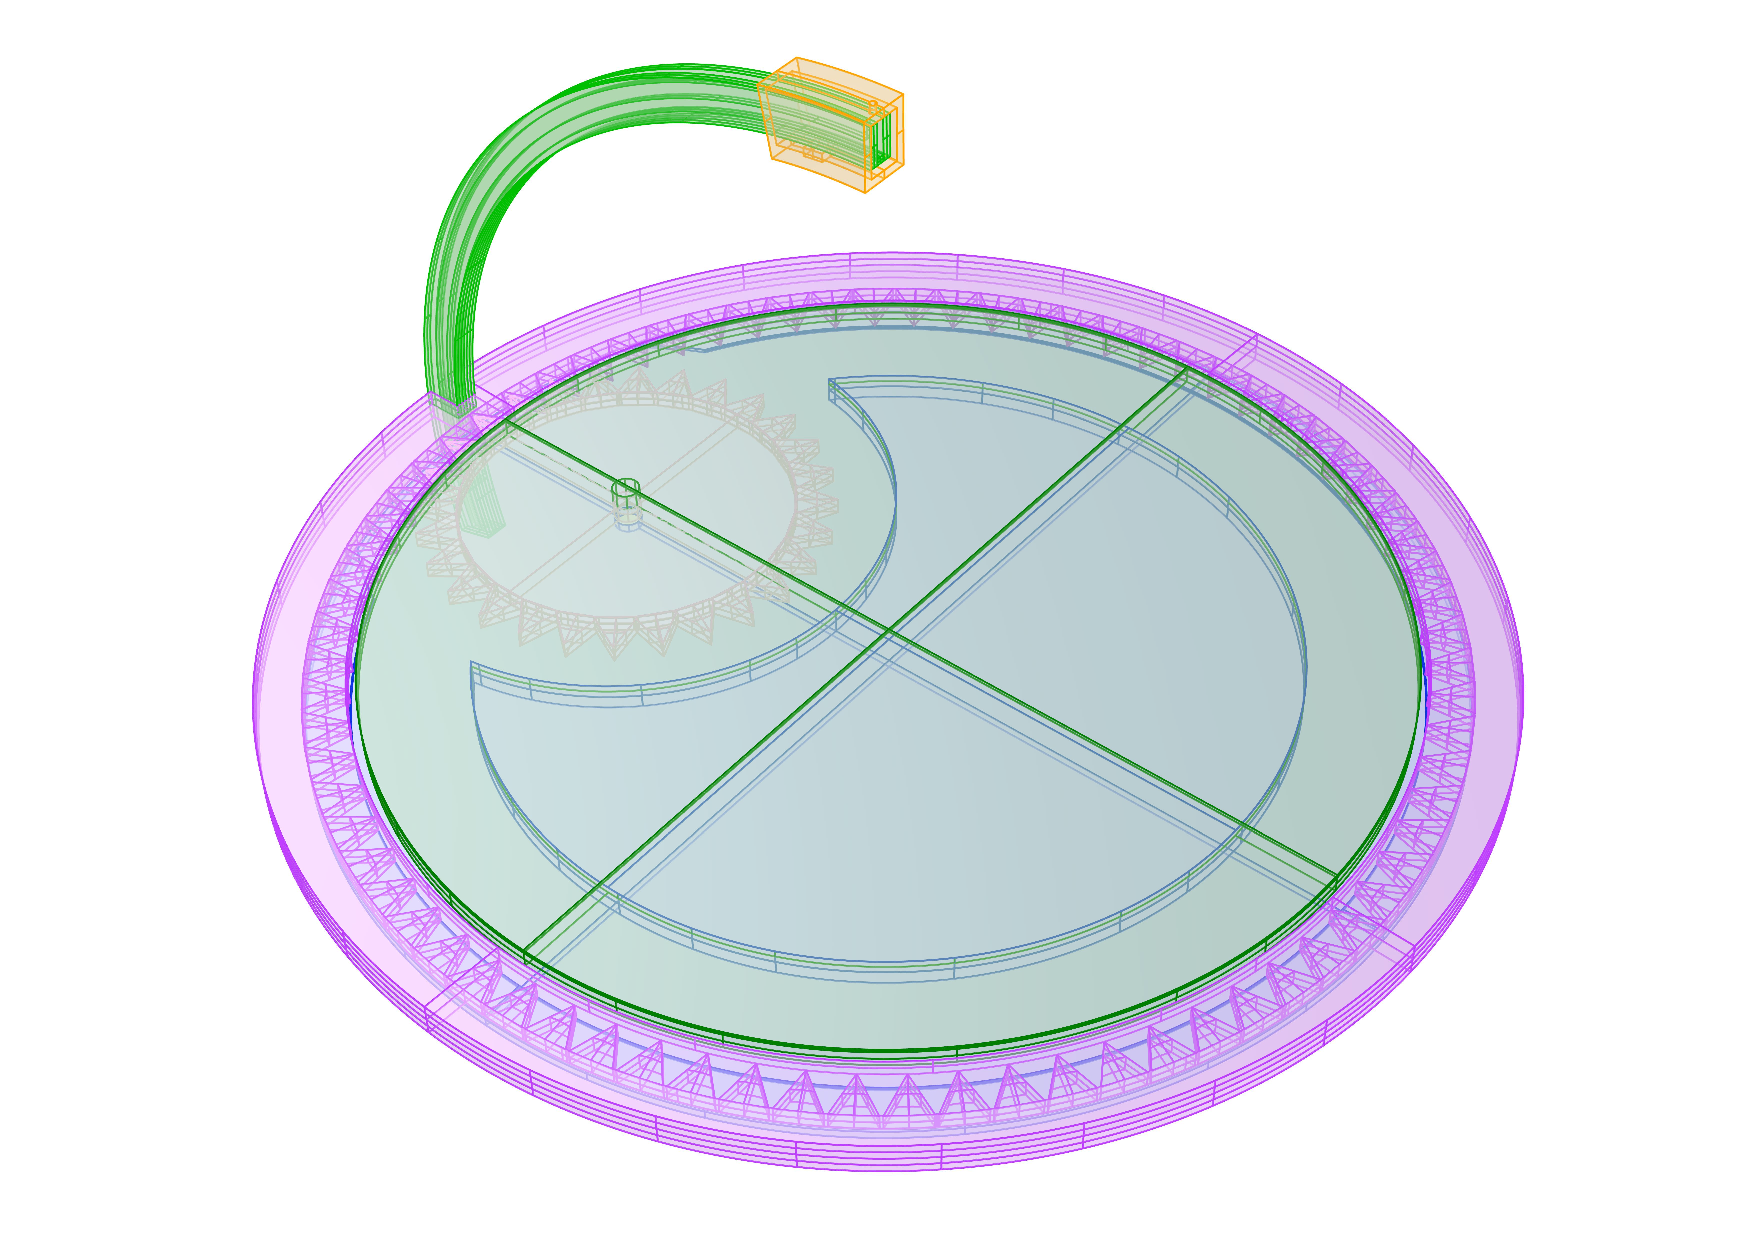
\includegraphics[width=.95\linewidth]{Images/2 axis prototype total.pdf}
       \\{Perspective of the mechanic}
         \label{sunpath}
    \end{minipage}
    \hfill
    \begin{minipage}{0.48\linewidth}
         \centering
        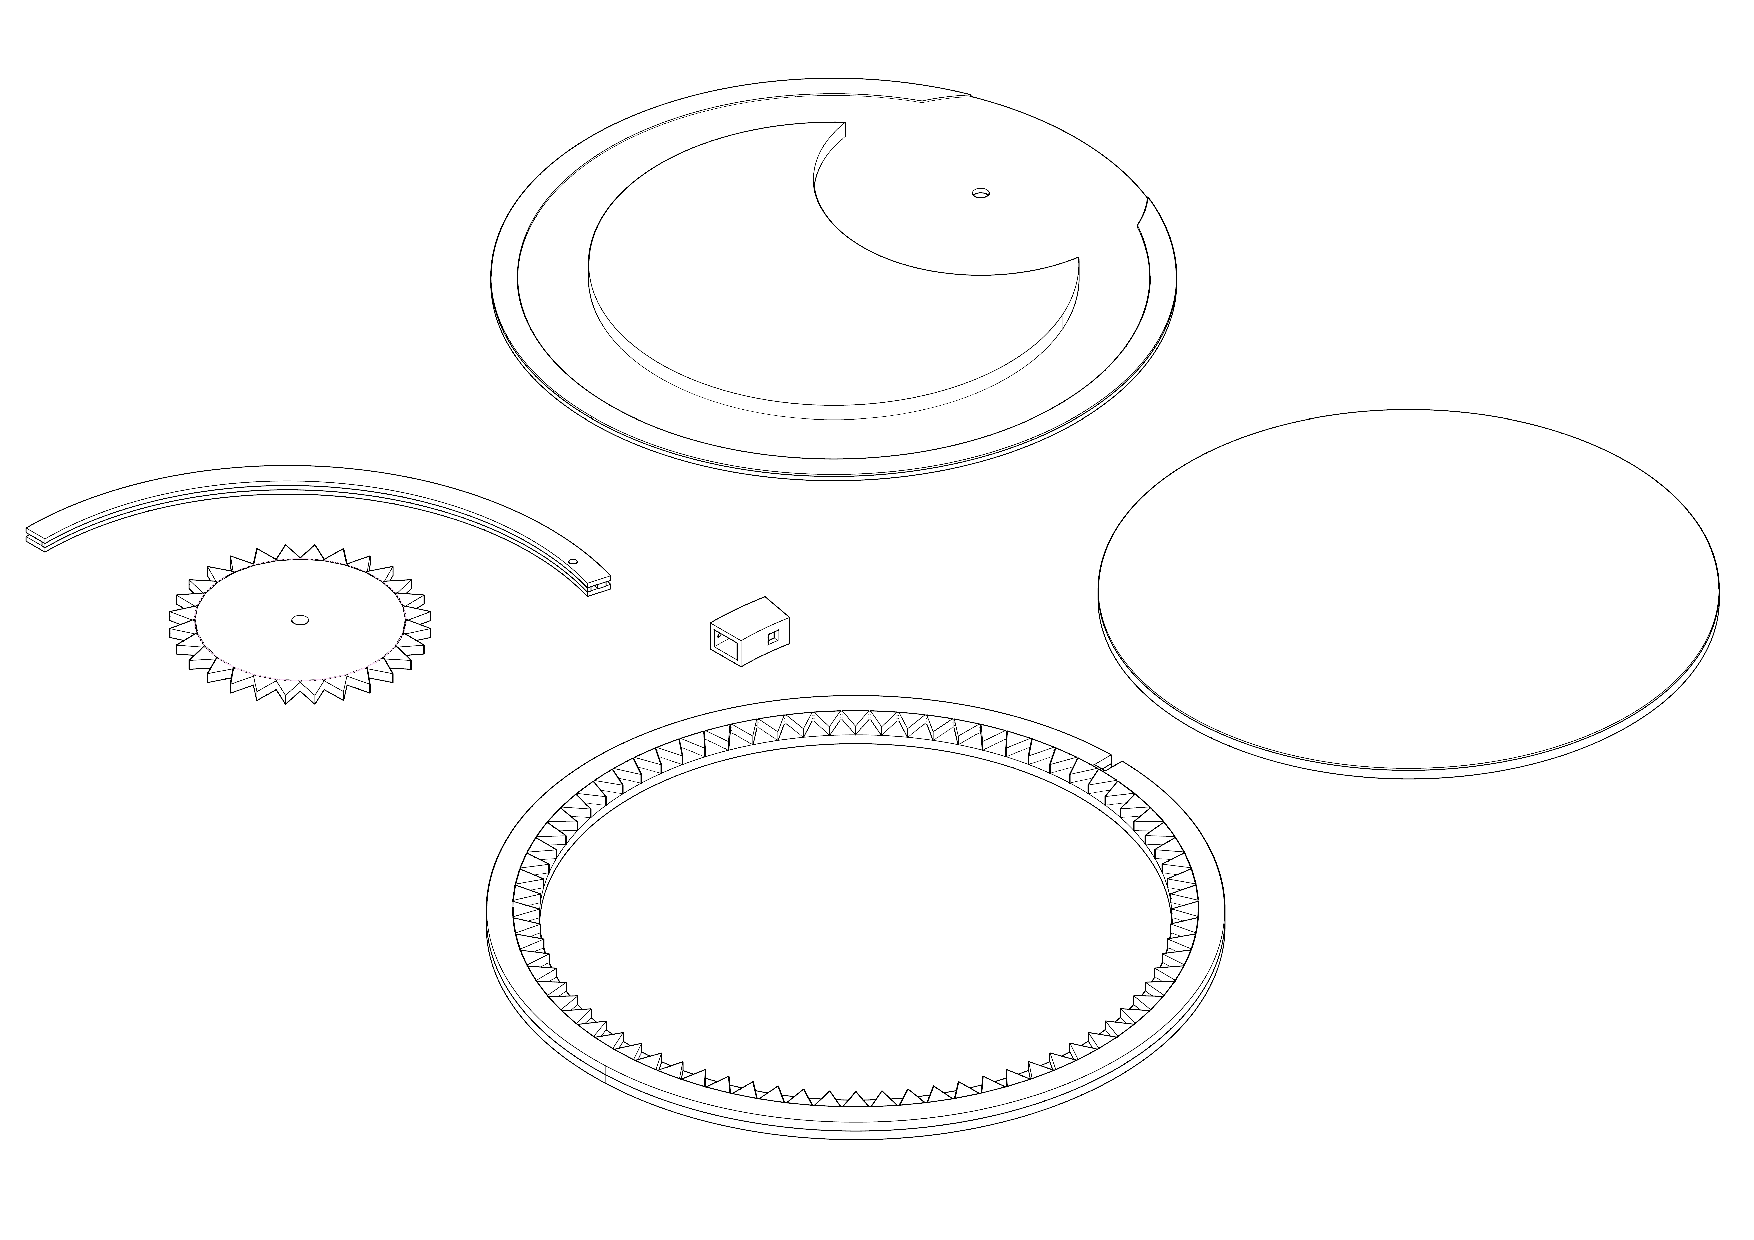
\includegraphics[width=.95\linewidth]{Images/2 axis prototype disect.pdf}
       \\{Individual Parts of the mechanic}
        \label{sunpath1}
    \end{minipage}
    \captionof{figure}{CAD plans of the horizontal coordinate system prototype}

    \begin{multicols}{2}
    [
    \subsubsection{"Sun path Coordinate System" Model }
    ]

    As seen in \textit{Section} \ref{hor}, it would be beneficial from an educational standpoint to have the sun path over a day clearly visible to the visitor. To do so, the movement of the sun over a day can be split differently. Namely into a offset of the path between the two solstices and a rotational movement along the path (cf. \textit{Figure} \ref{pathcoord}). Let us call this reference system the "sun path coordinate system".\\
    \\
    However, this brings the disadvantage, that it leads to a presence of the path below the model surface for some positions, as the winter season has shorter paths than the summer season. This leads to more space needed below the model. To prevent that, in a first attempt a prototype was created working with a bendable circle (here nylon wire, in a larger scale probably spring steel rod) representing the sun path, which was fixed on the underside and shortened or lengthened using a slider (cf. \textit{Figure} \ref{protobend}). The slider could potentially be moved back and forth using a gear and rack system. (cf. implementation in \textit{Figure} \ref{caddd}). This system could be scaled up using a spring steel rod to recreate the bending behaviour of the nylon wire. However such a slider mechanism, which changes the exposed length of the system, makes the rotational movement of the path very difficult to control and implement because of the bending. Therefore a system without the bending of the sun path circle was explored.

   
    \end{multicols}

    \begin{minipage}{0.48\linewidth}
         \begin{figure}[H]
        \centering
        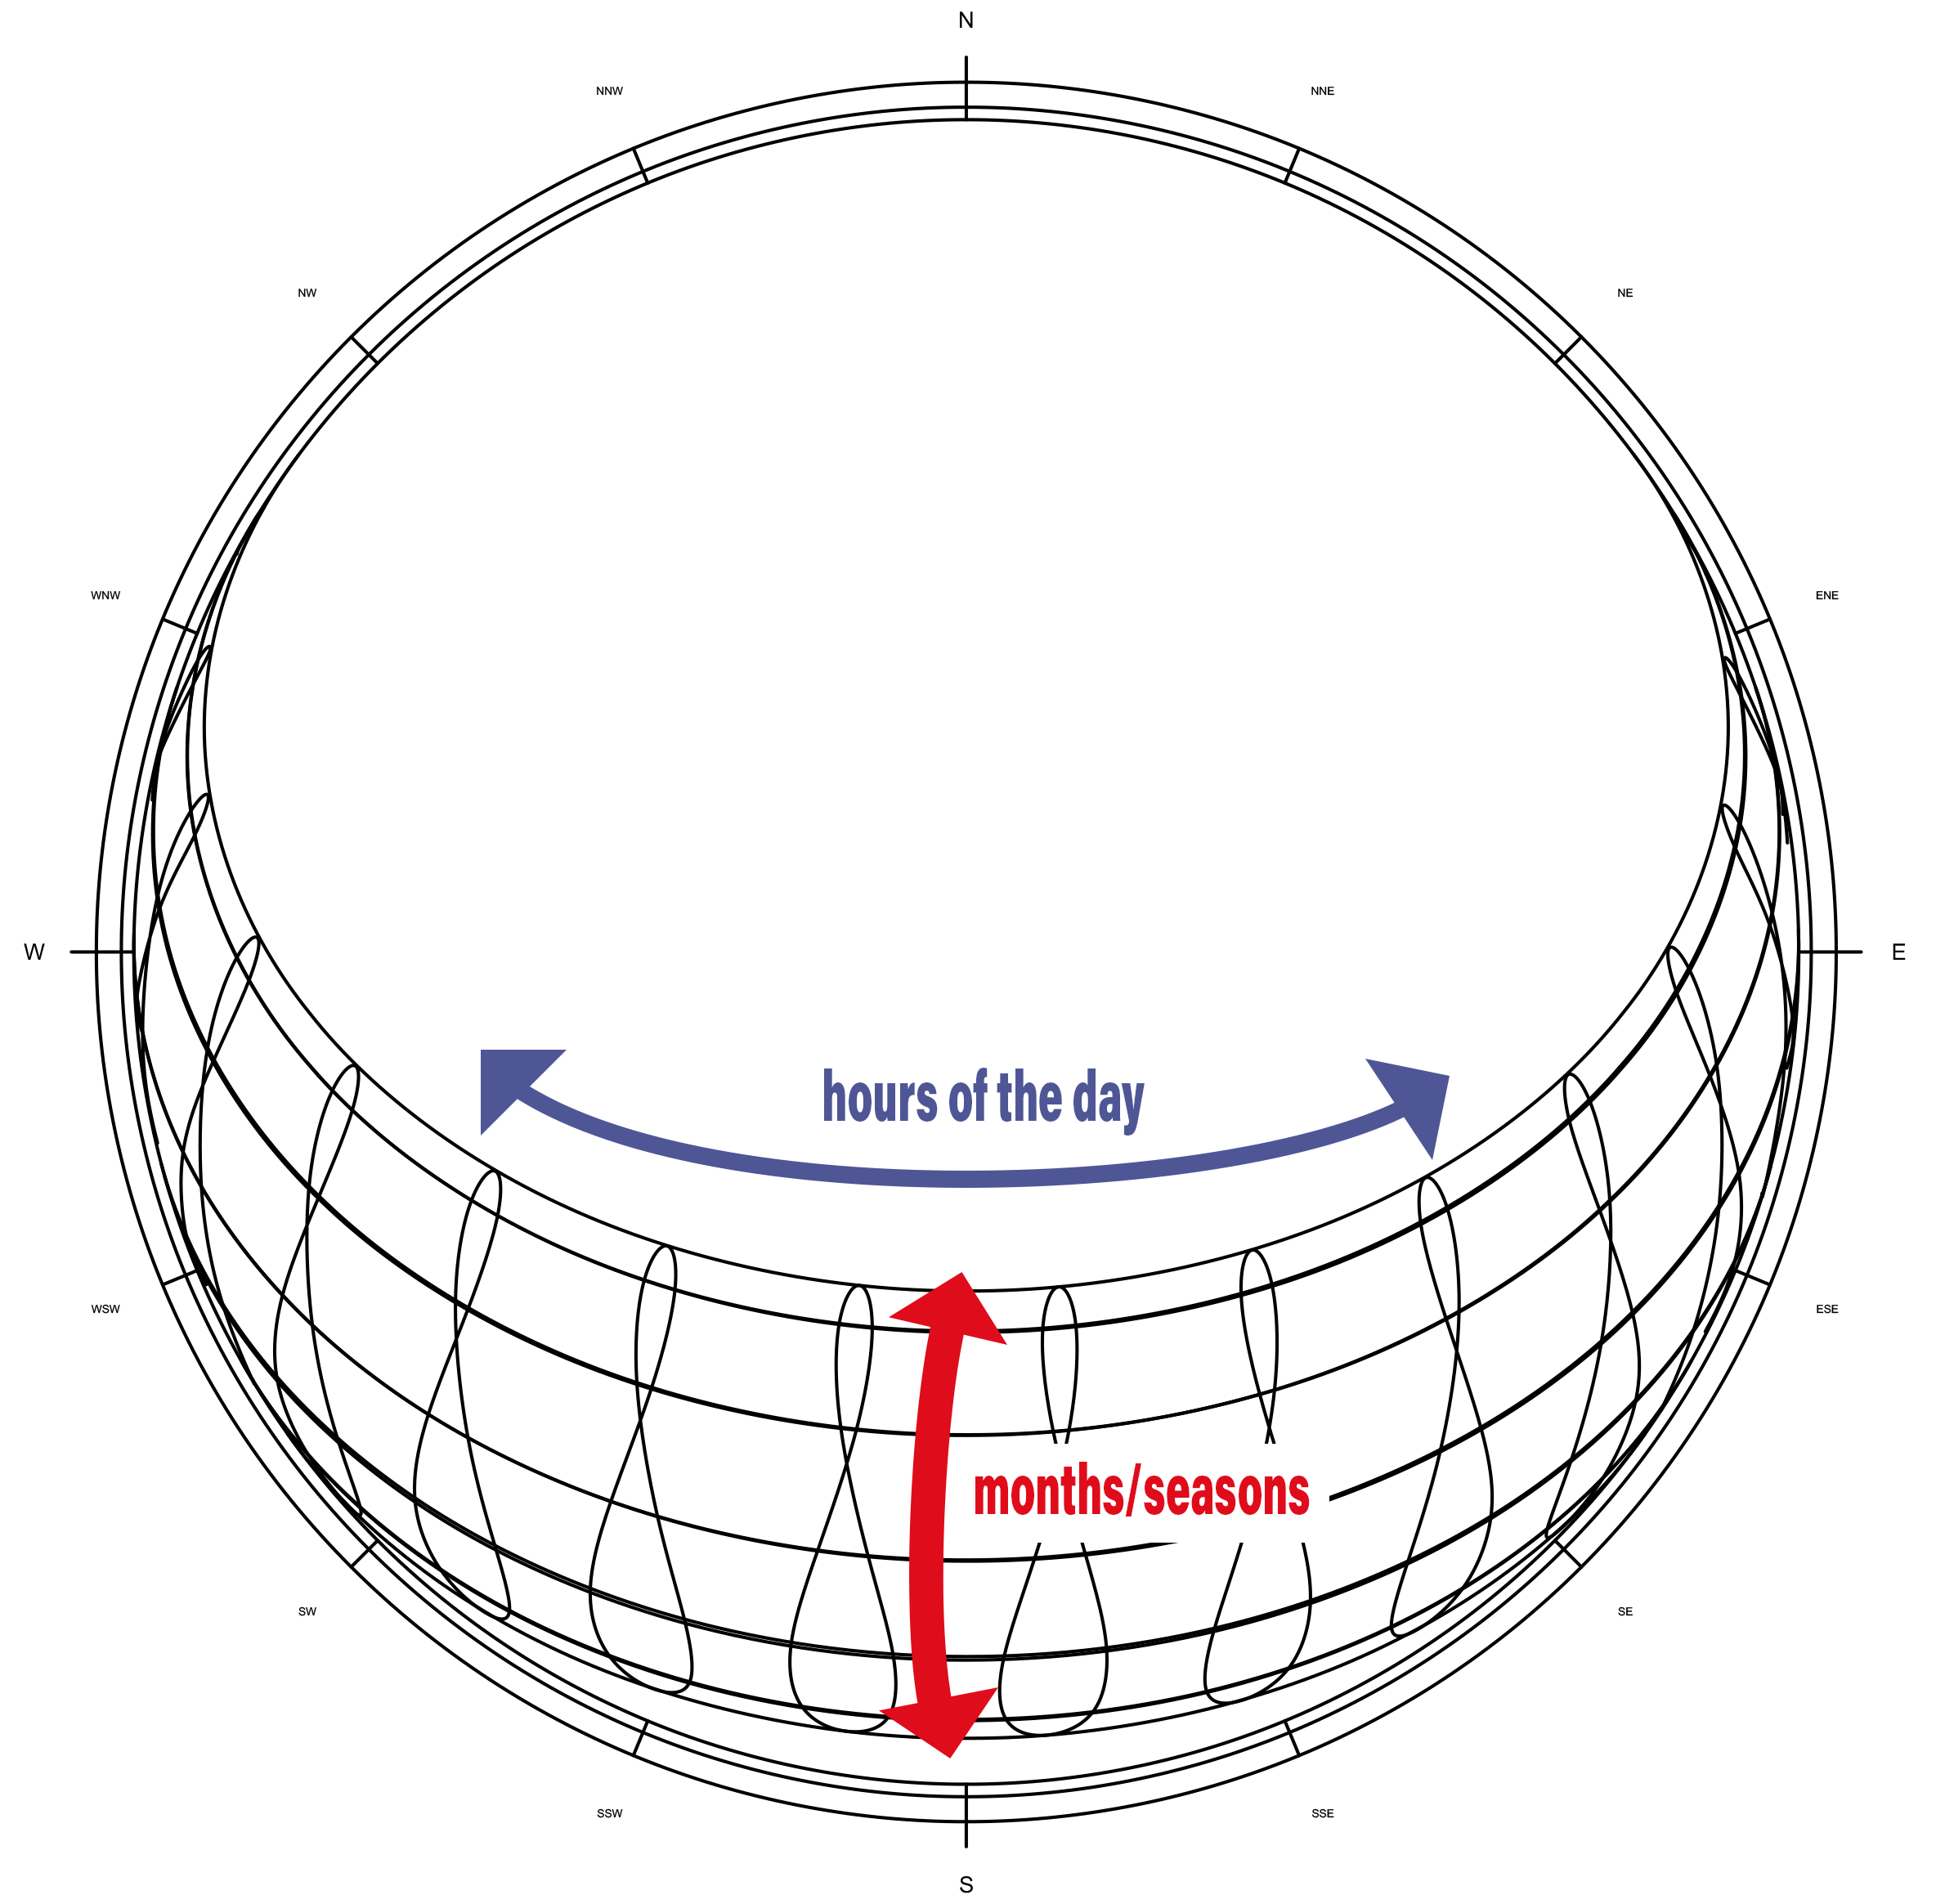
\includegraphics[width=.7\linewidth]{Images/sun path coord.png}
        \captionof{figure}{The "sun path coordinate system"}
        \label{pathcoord}
    \end{figure}
    \end{minipage}
    \hfill
    \begin{minipage}{0.48\linewidth}
         \begin{figure}[H]
        \centering
        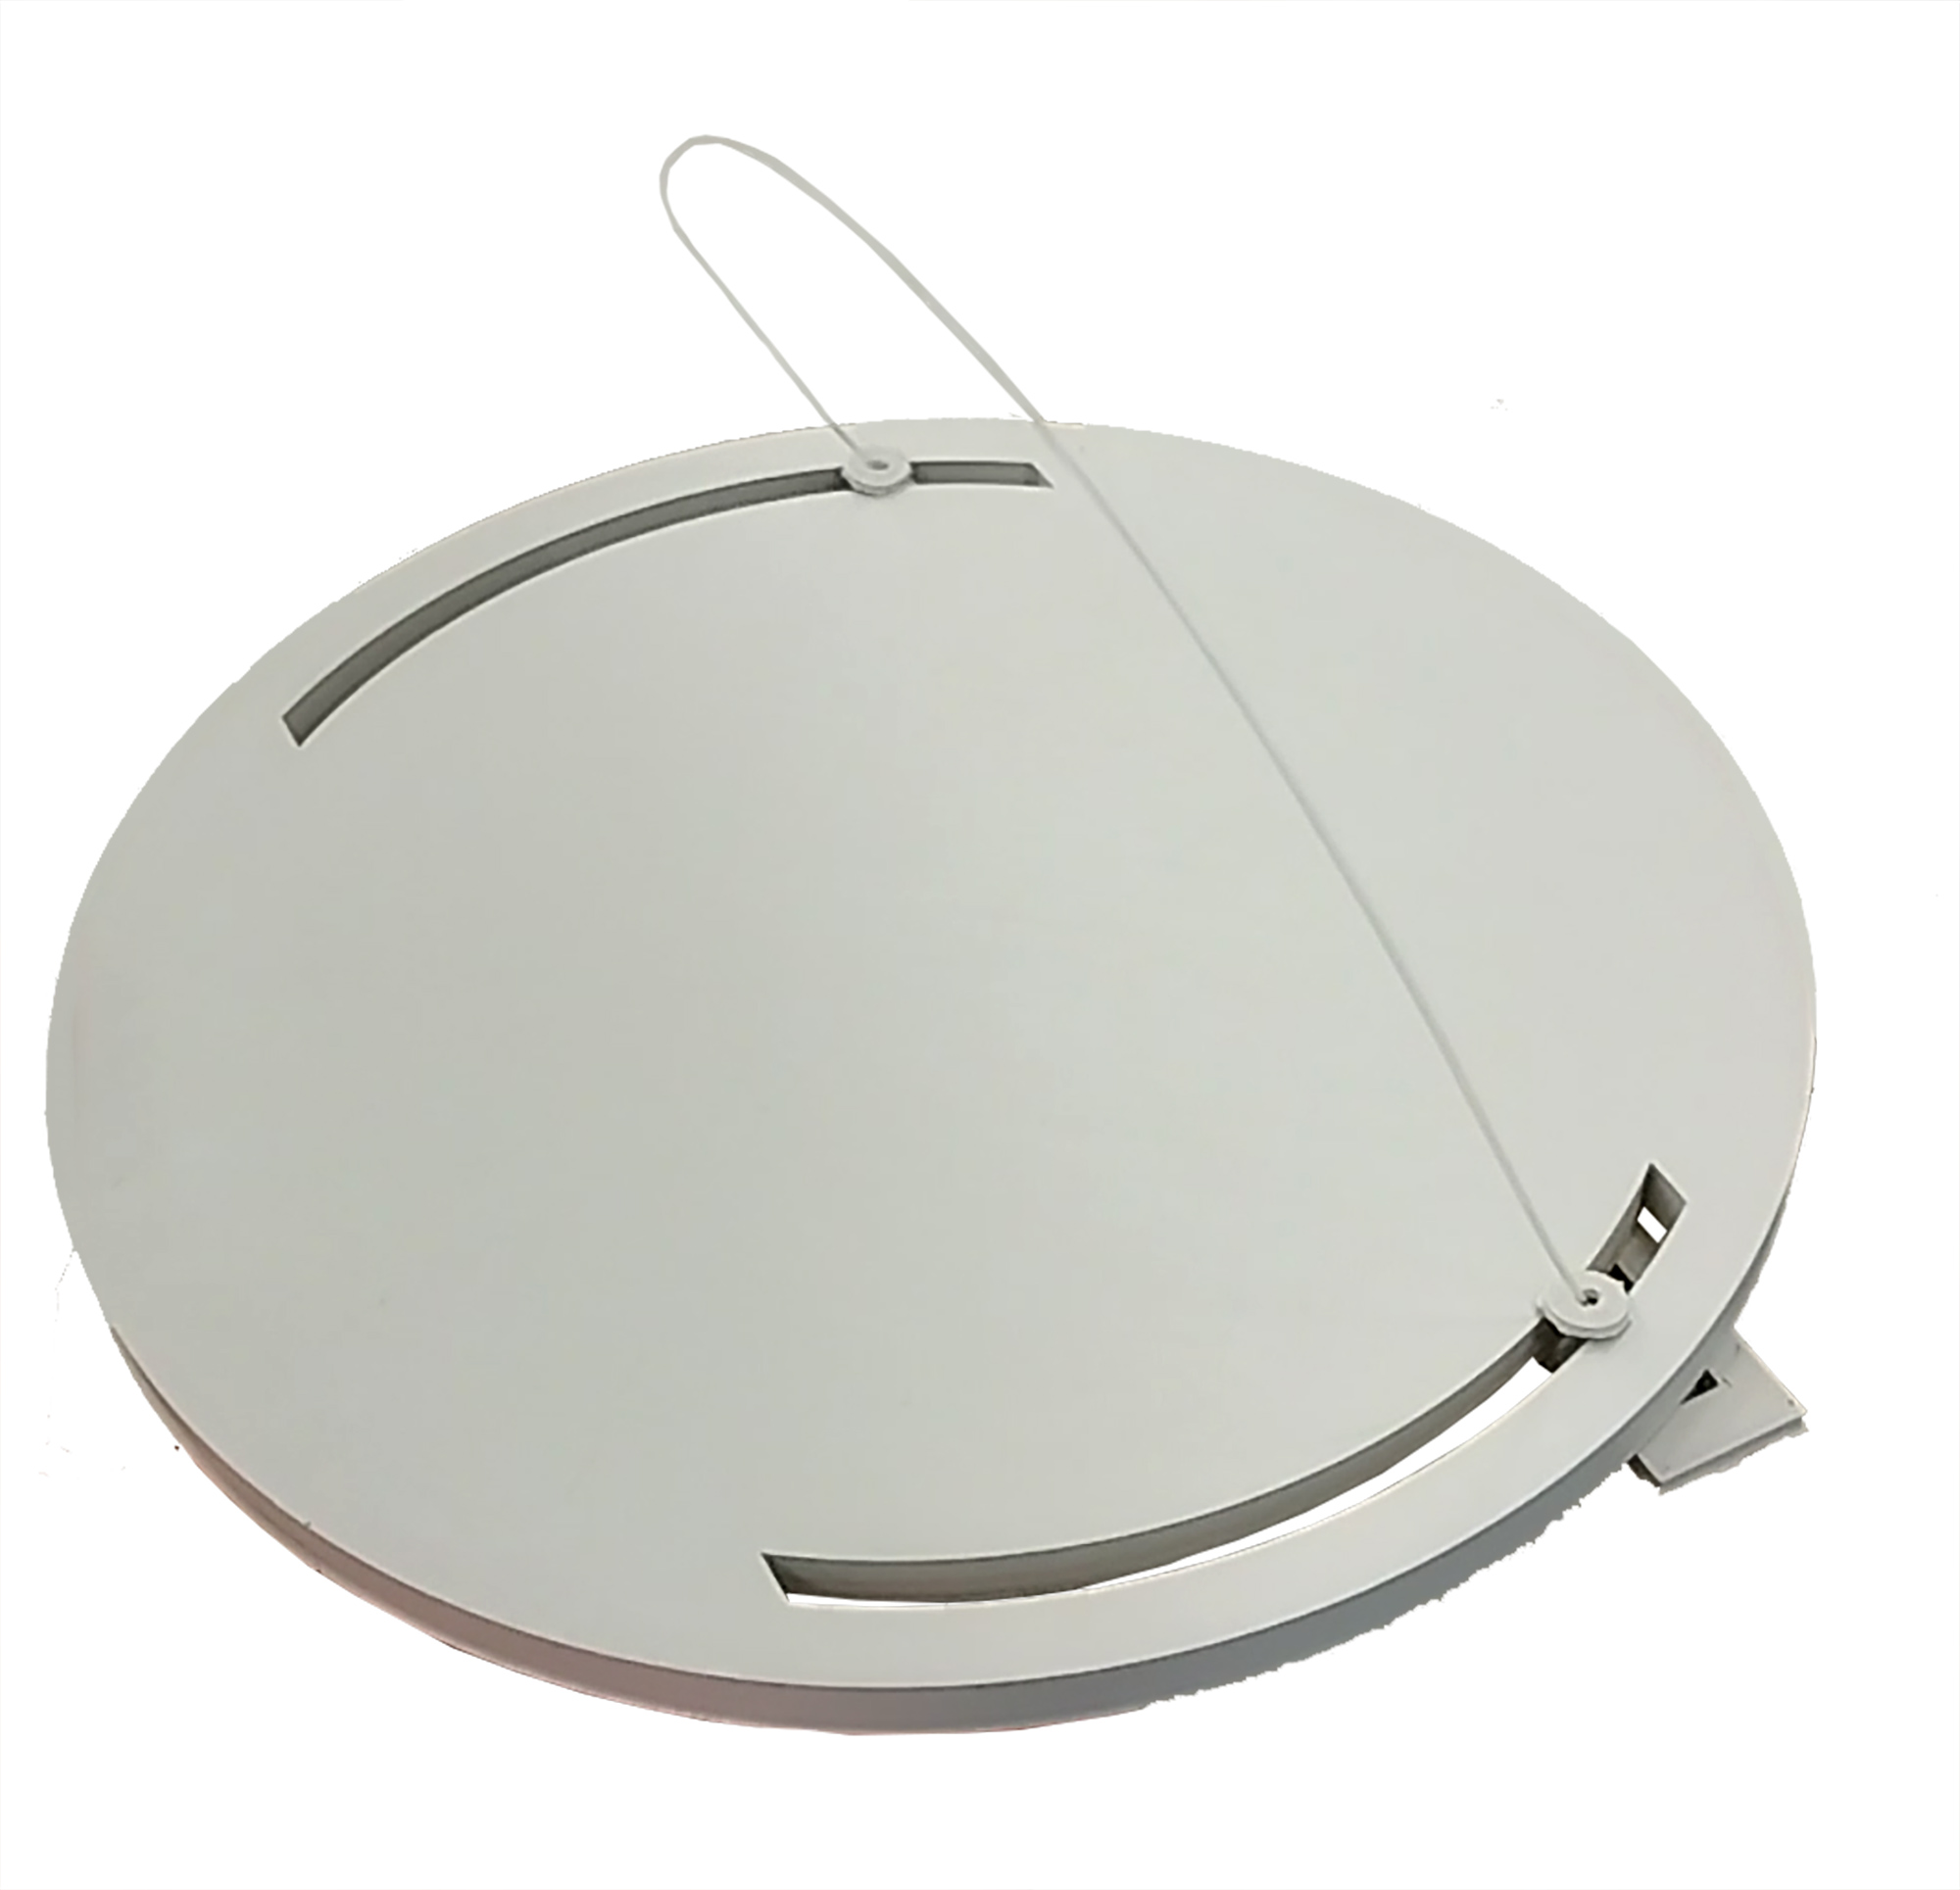
\includegraphics[width=.7\linewidth]{Images/prototyp bending v22_1.jpg}
        \captionof{figure}{Fully functional prototype using an sun path which can be offset}
        \label{protobend}
    \end{figure}
    \end{minipage}
    \captionof{figure}{CAD plans of the horizontal coordinate system prototype}
    \footnotetext{\footcite{horzontalcooorindatesources}}
    \vspace{.9cm}
    \begin{minipage}{0.48\linewidth}
        \centering
        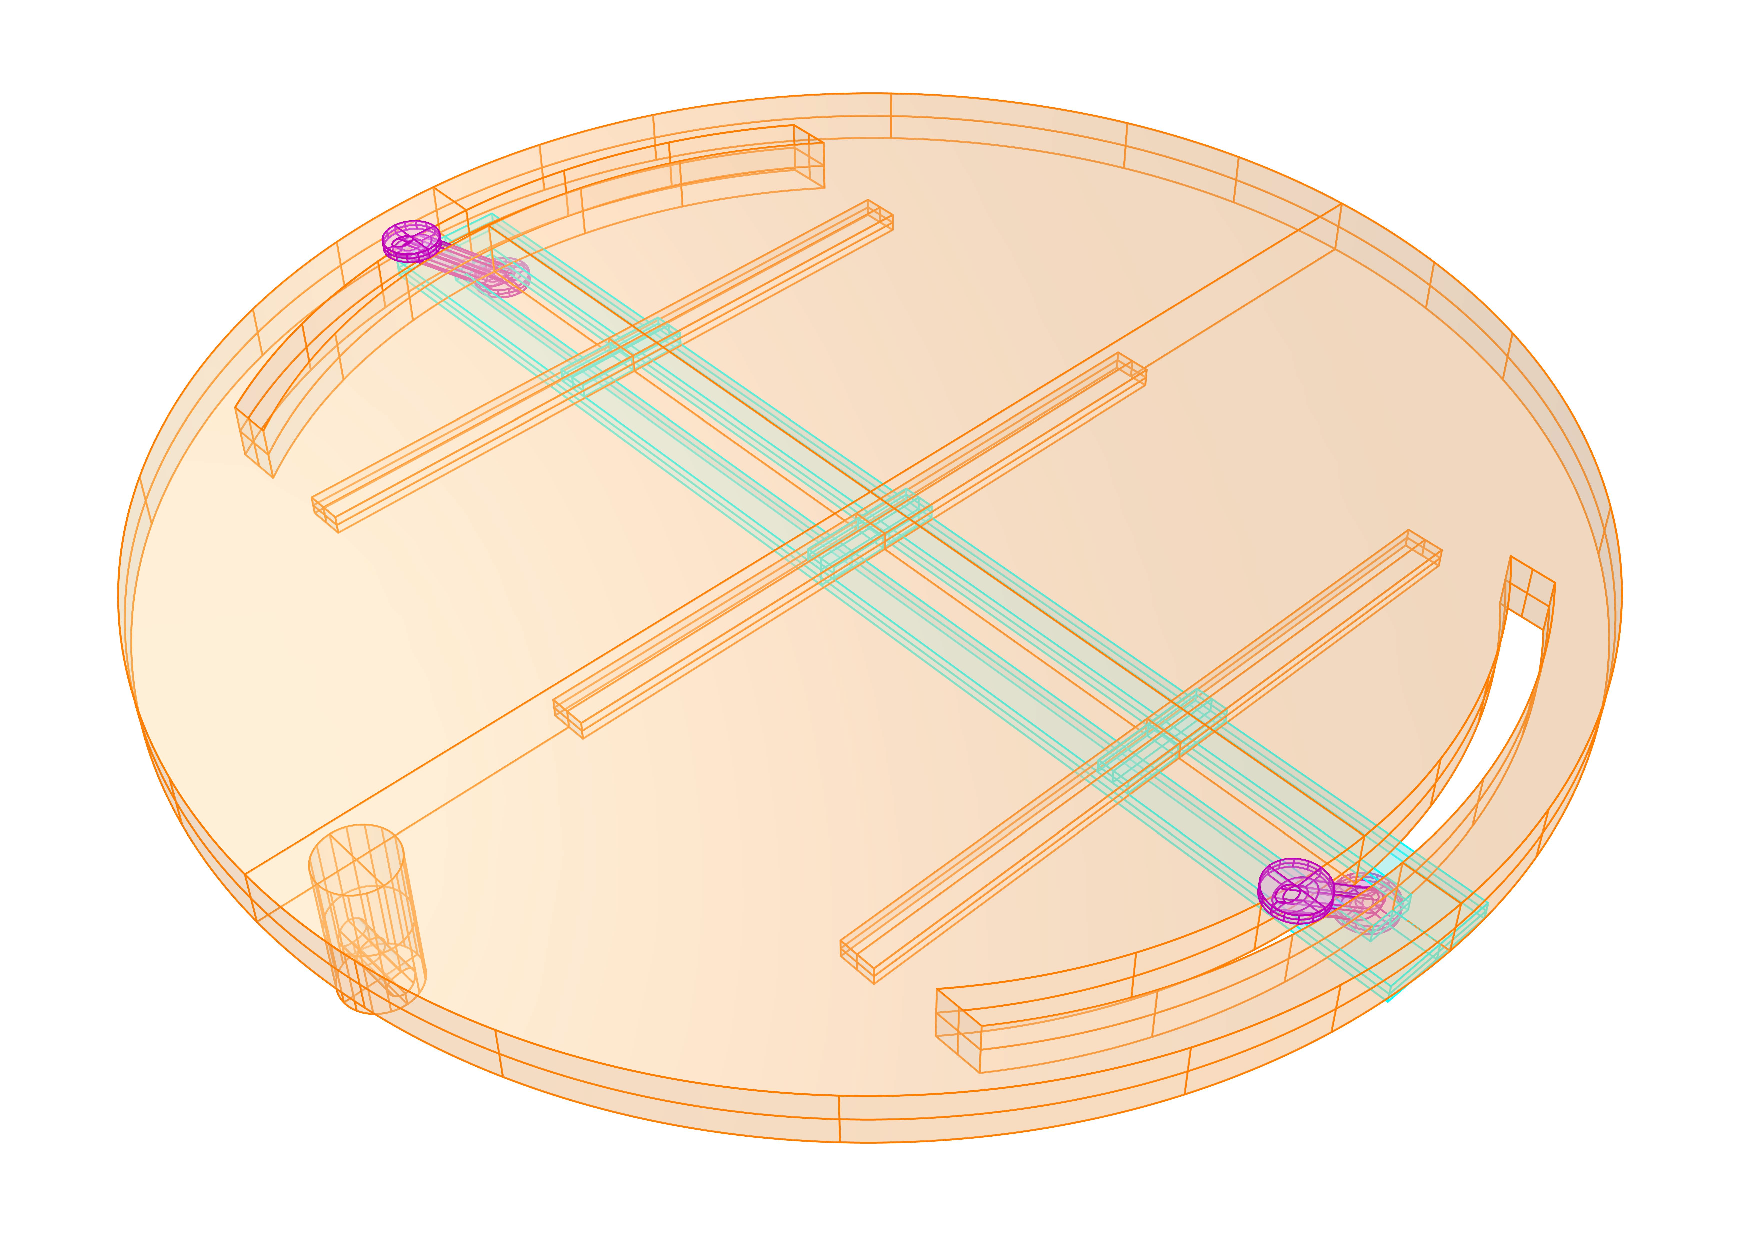
\includegraphics[width=.85\linewidth]{Images/ring prototype_v1 - total.pdf}
       \\{Perspective of the mechanic}
         \label{sunpath}
    \end{minipage}
    \hfill
    \begin{minipage}{0.48\linewidth}
         \centering
        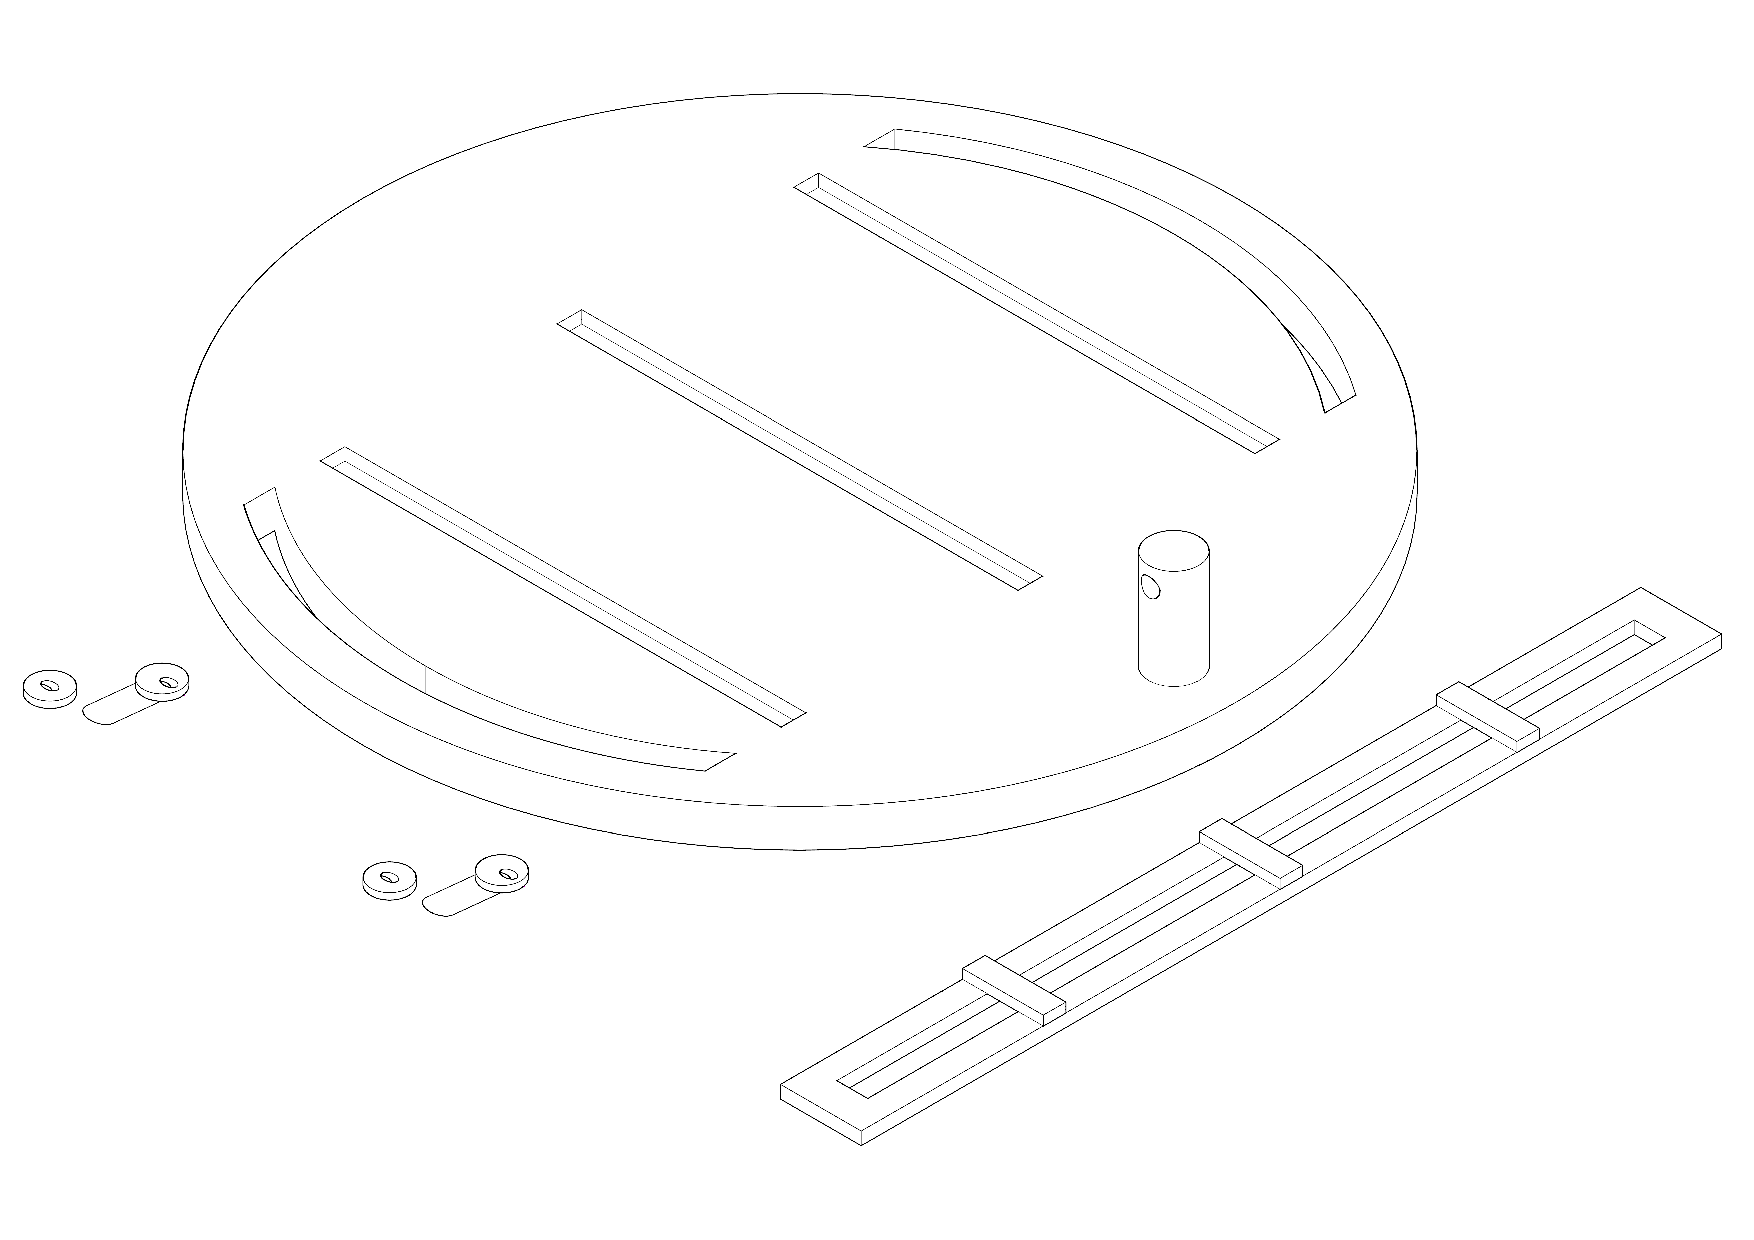
\includegraphics[width=.85\linewidth]{Images/ring prototype_v1 - disect.pdf}
       \\{Individual Parts of the mechanic}
        \label{sunpath1}
    \end{minipage}
    \captionof{figure}{CAD plans of the horizontal coordinate system prototype}
    \label{sli}
\newpage
\begin{multicols}{2}
    [
    \subsubsection{"Sun path Coordinate" - a second attempt }
    ]
     Starting from this challenge, another prototype was developed. In this version, the ring is reduced to the part of the path, which is fully exposed in the most extreme position (june 21$^{st}$). This allows to reduce the space which is needed underneath the model compared to a version, where the path is implemented as a full circle. Below the model a stepper motor is placed using a threaded rod to move the path "up and down" (cf. \textit{Figure} \ref{setupp}). To hide the space needed for this mechanical setup, a cover on top of the table would be needed. For example by angling the information texts towards the visitor and creating a plinth for the model (cf. \textit{Figure} \ref{table}). This plinth will host and cover the mechanical assembly, such that it is not visible from the visitors point of view. The rotational movement would be realised with a wagon, which is clamped to the path and slides along the ring. \\
     \\
     The major downside of such an assembly is, that the movement of the wagon is easily realizable but very hard to control, as the path changes its length over the seasons. Thus, there is no properly defined end position of the path and as a result no good space for an end switch to determine/reset the stepper motors position. Due to these complexities with this strategy, another strategy was chosen in the end.
\end{multicols}




    \begin{minipage}{0.48\linewidth}
       \begin{figure}[H]
        \centering
        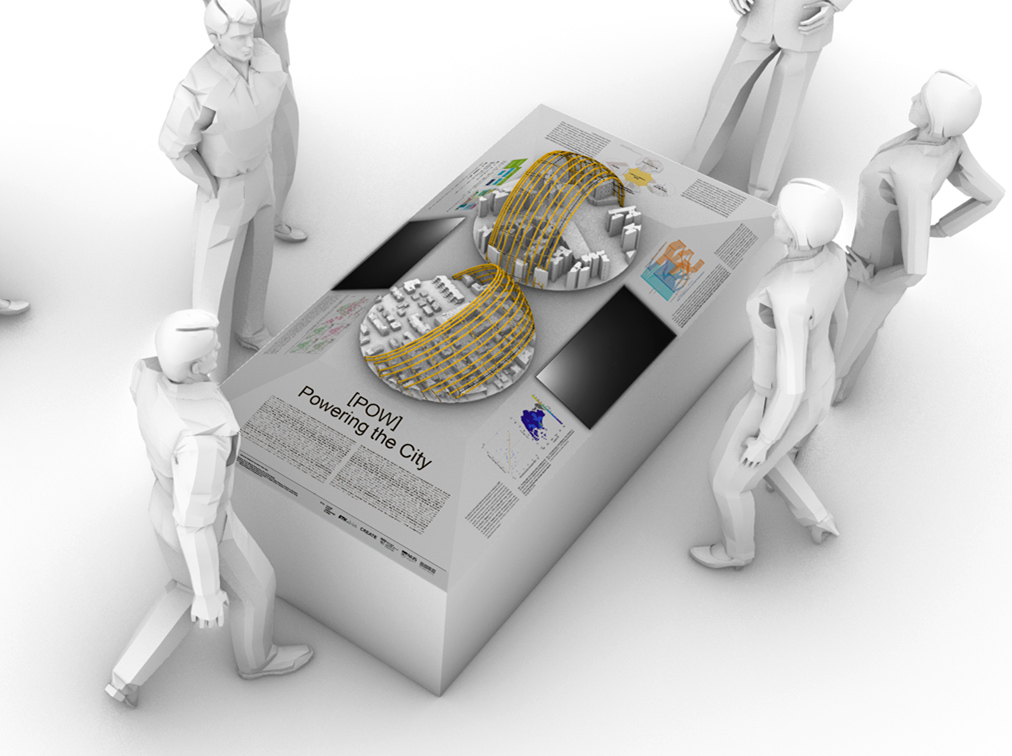
\includegraphics[width=\linewidth]{Images/table_1.jpg}
        \caption{Example setup of the table with a plinth}
        \label{table}
    \end{figure}
    \end{minipage}
    \hfill
    \begin{minipage}{0.48\linewidth}
       \begin{figure}[H]
        \centering
        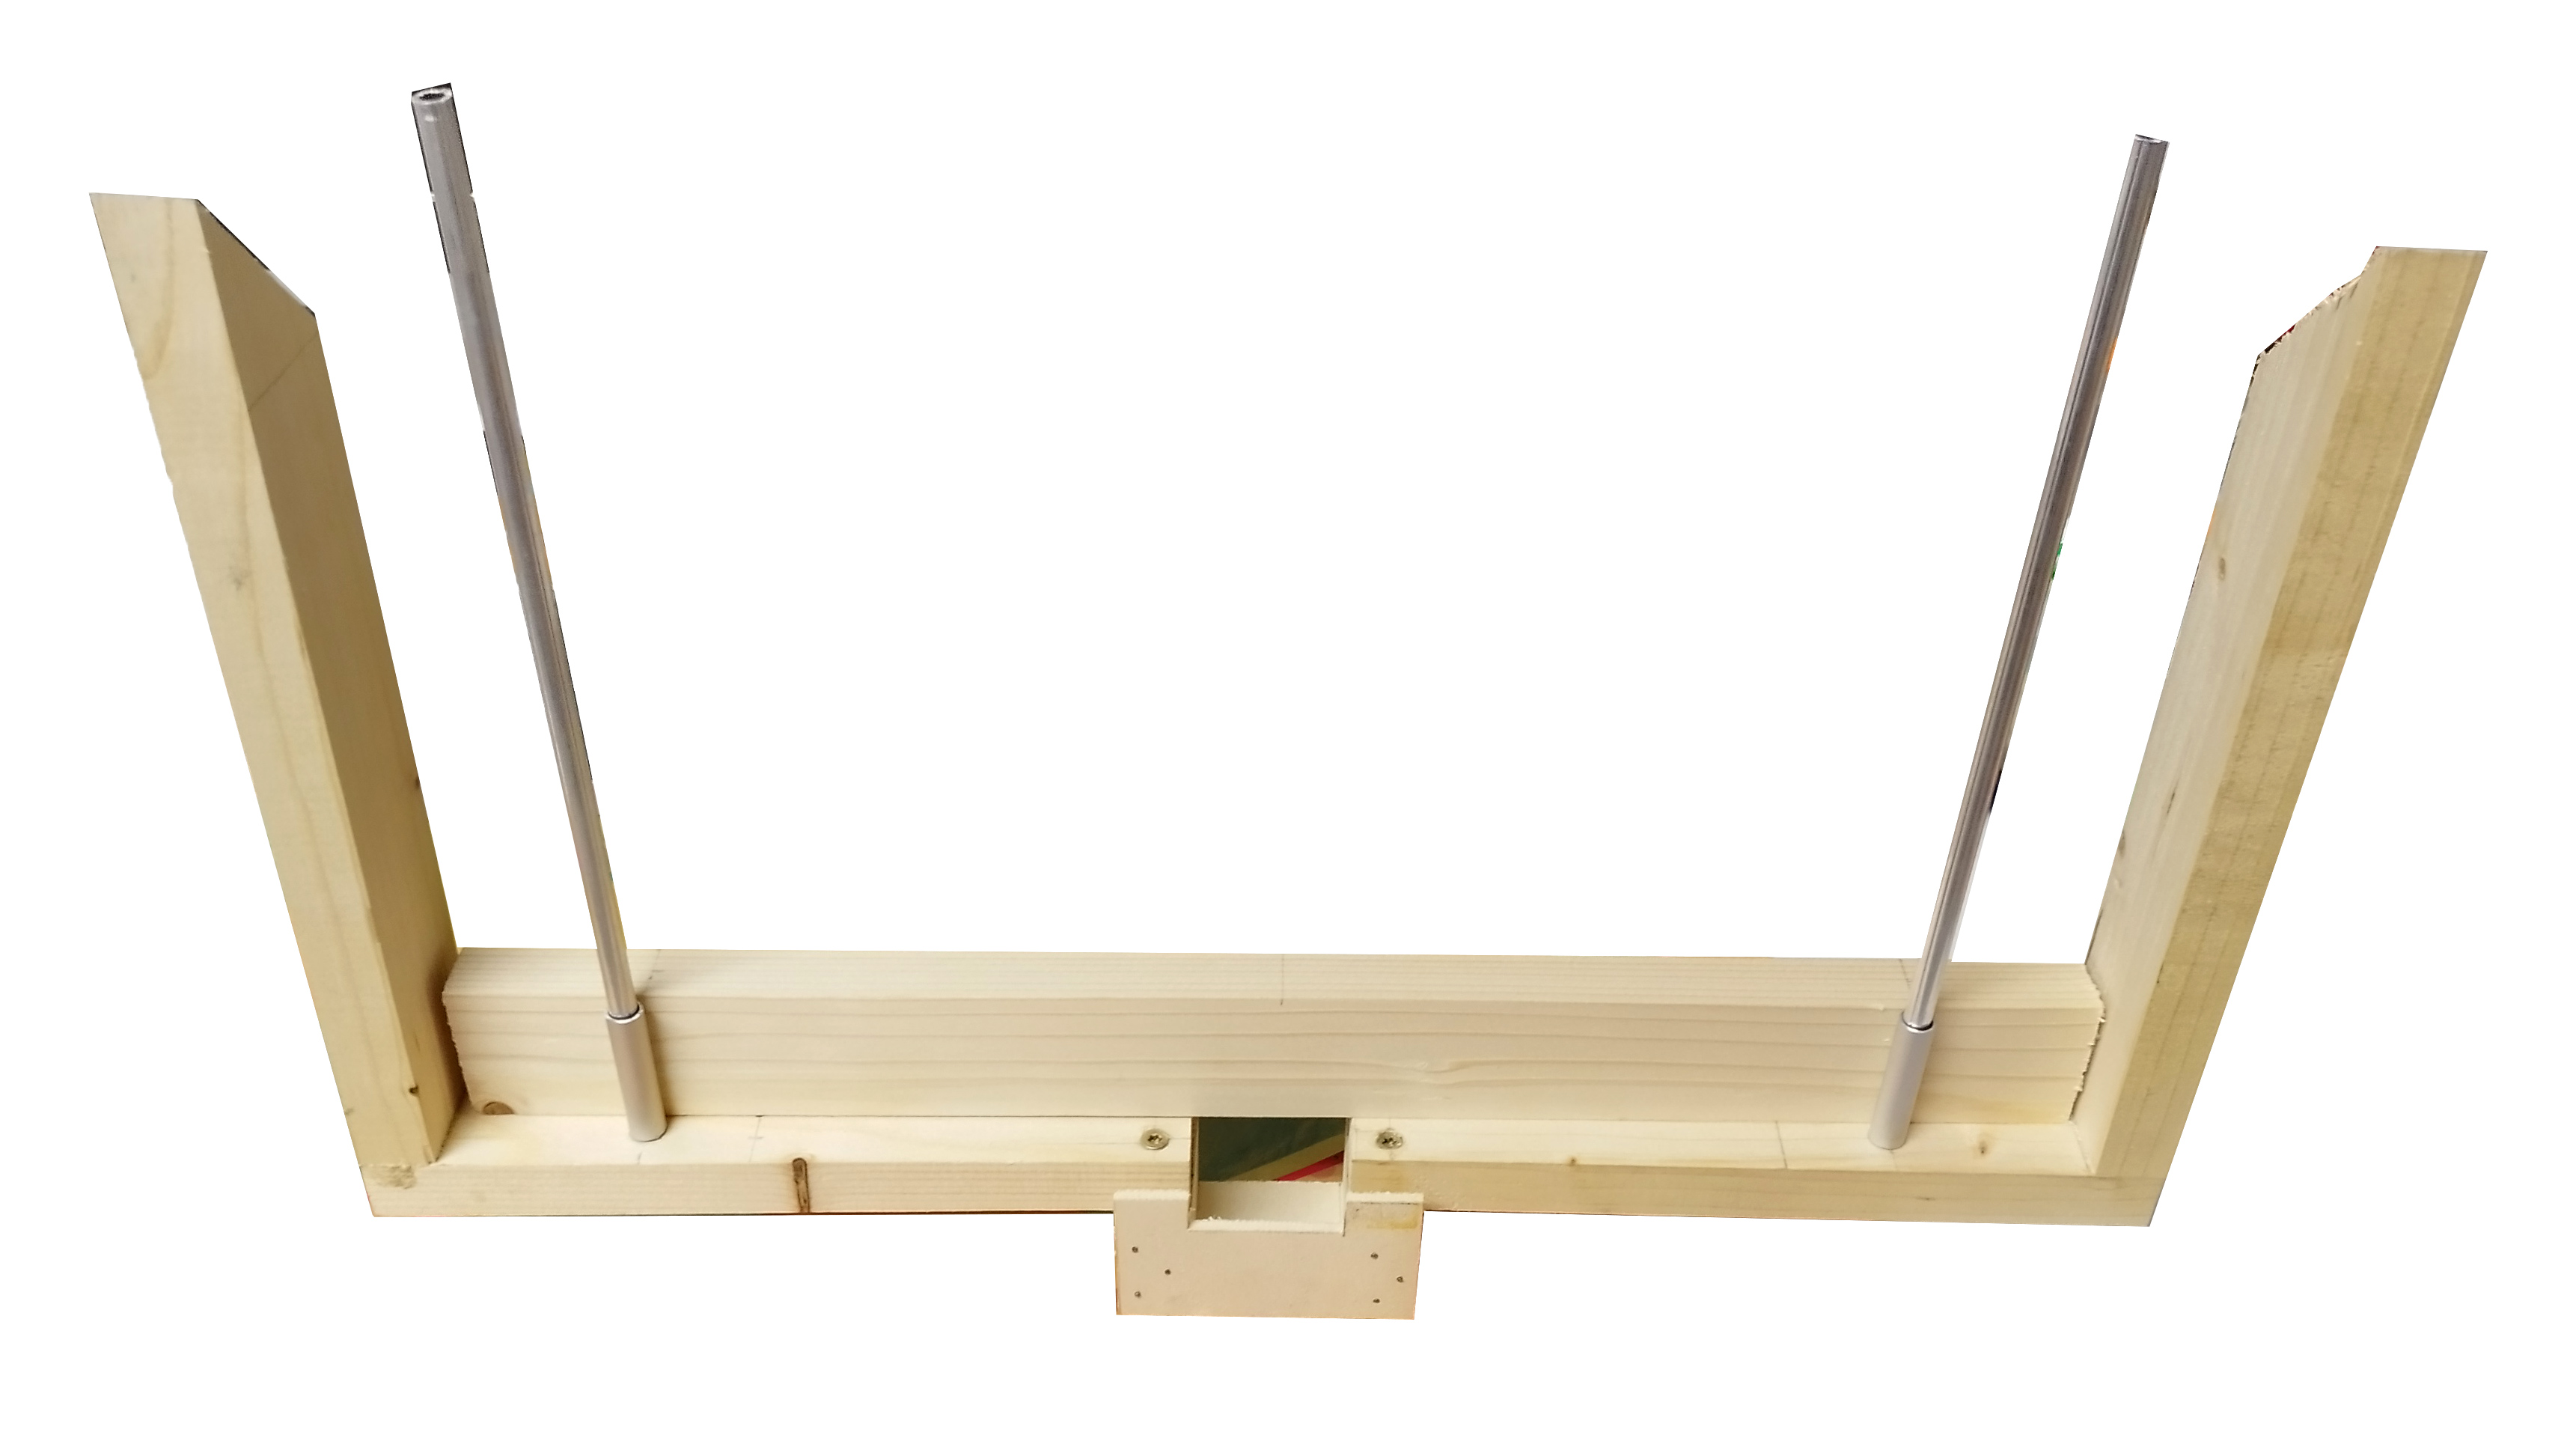
\includegraphics[width=\linewidth]{Images/Slider_1.jpg}
        \caption{Slider setup which would be driven up and down by threaded rod and stepper motor}
        \label{setupp}
    \end{figure}
    \end{minipage}
    
     \begin{minipage}{0.48\linewidth}
        \centering
        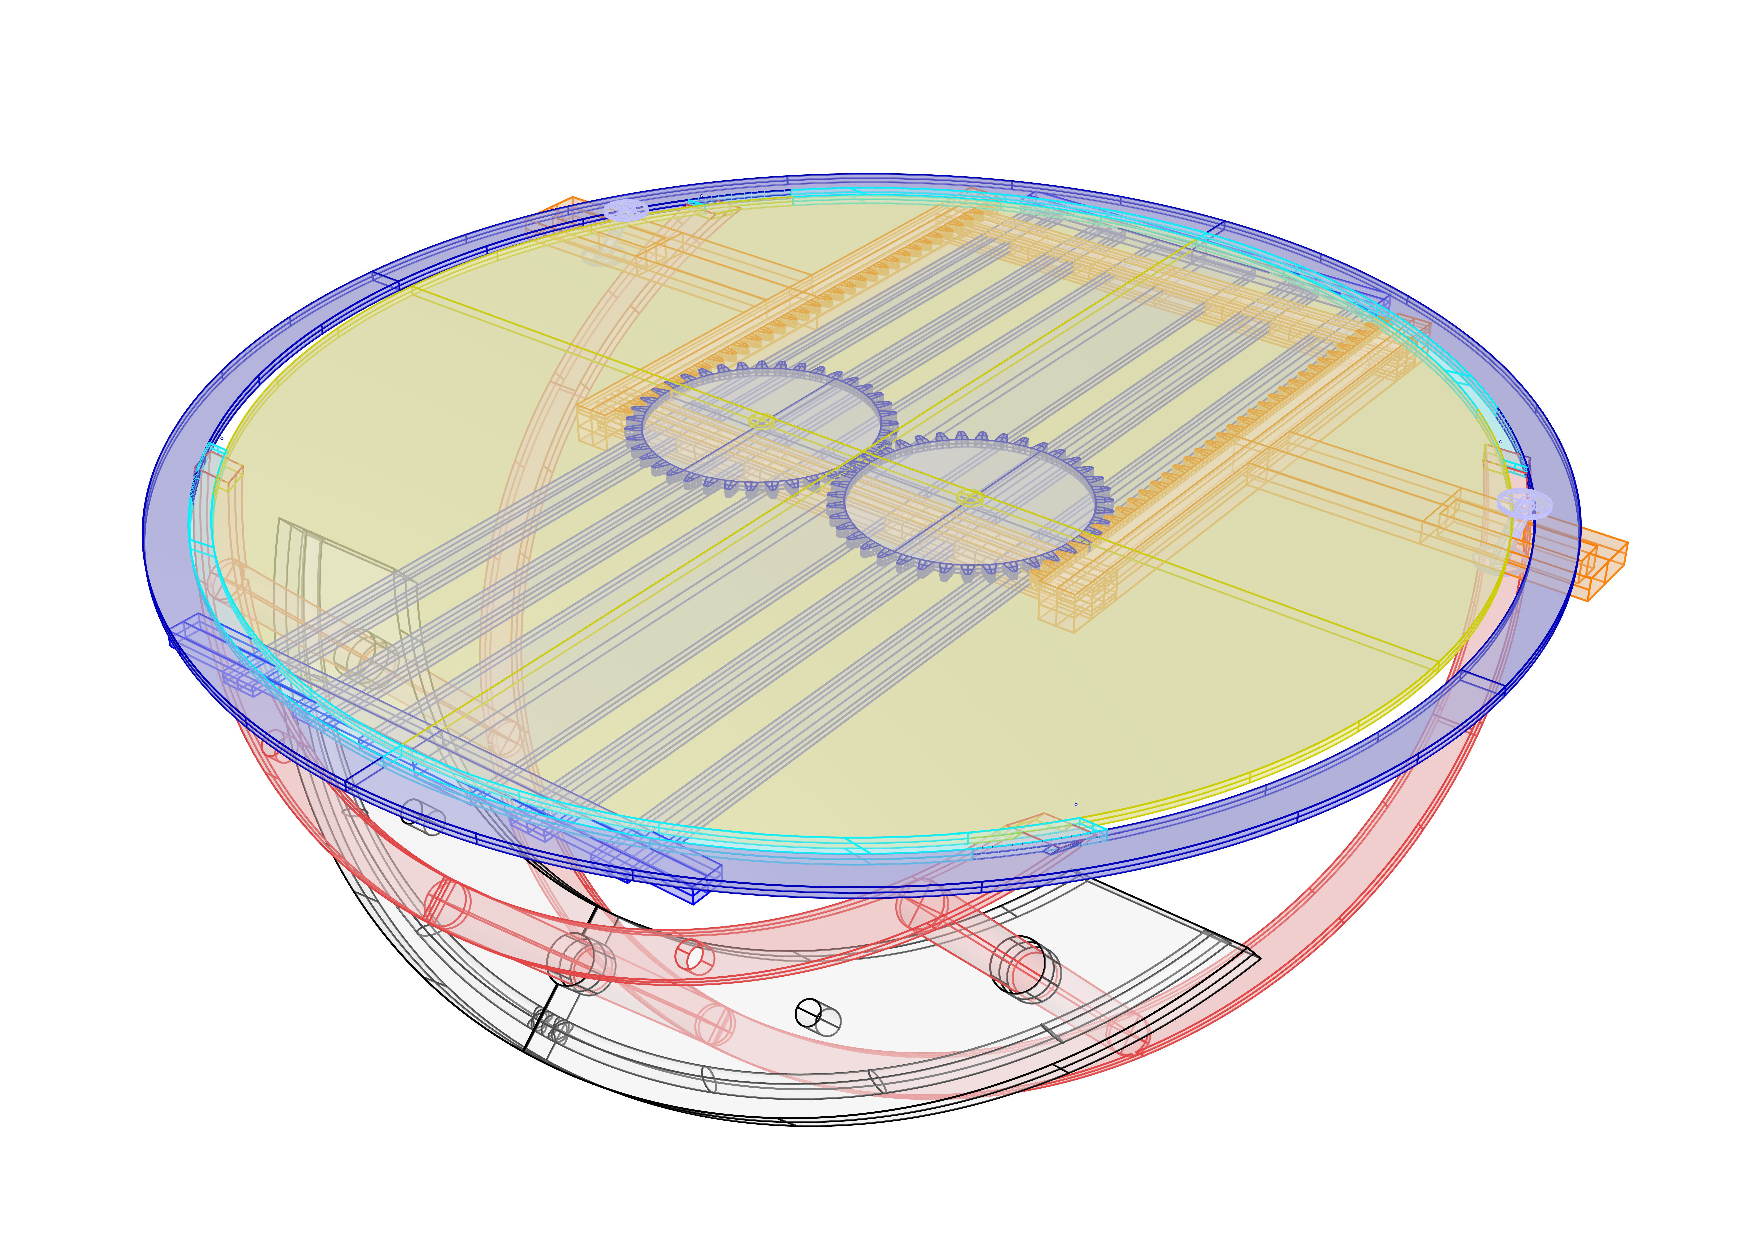
\includegraphics[width=.85\linewidth]{Images/ring prototype_v2 total.pdf}
       \\{Perspective of the mechanic}
       
    \end{minipage}
    \hfill
    \begin{minipage}{0.48\linewidth}
         \centering
        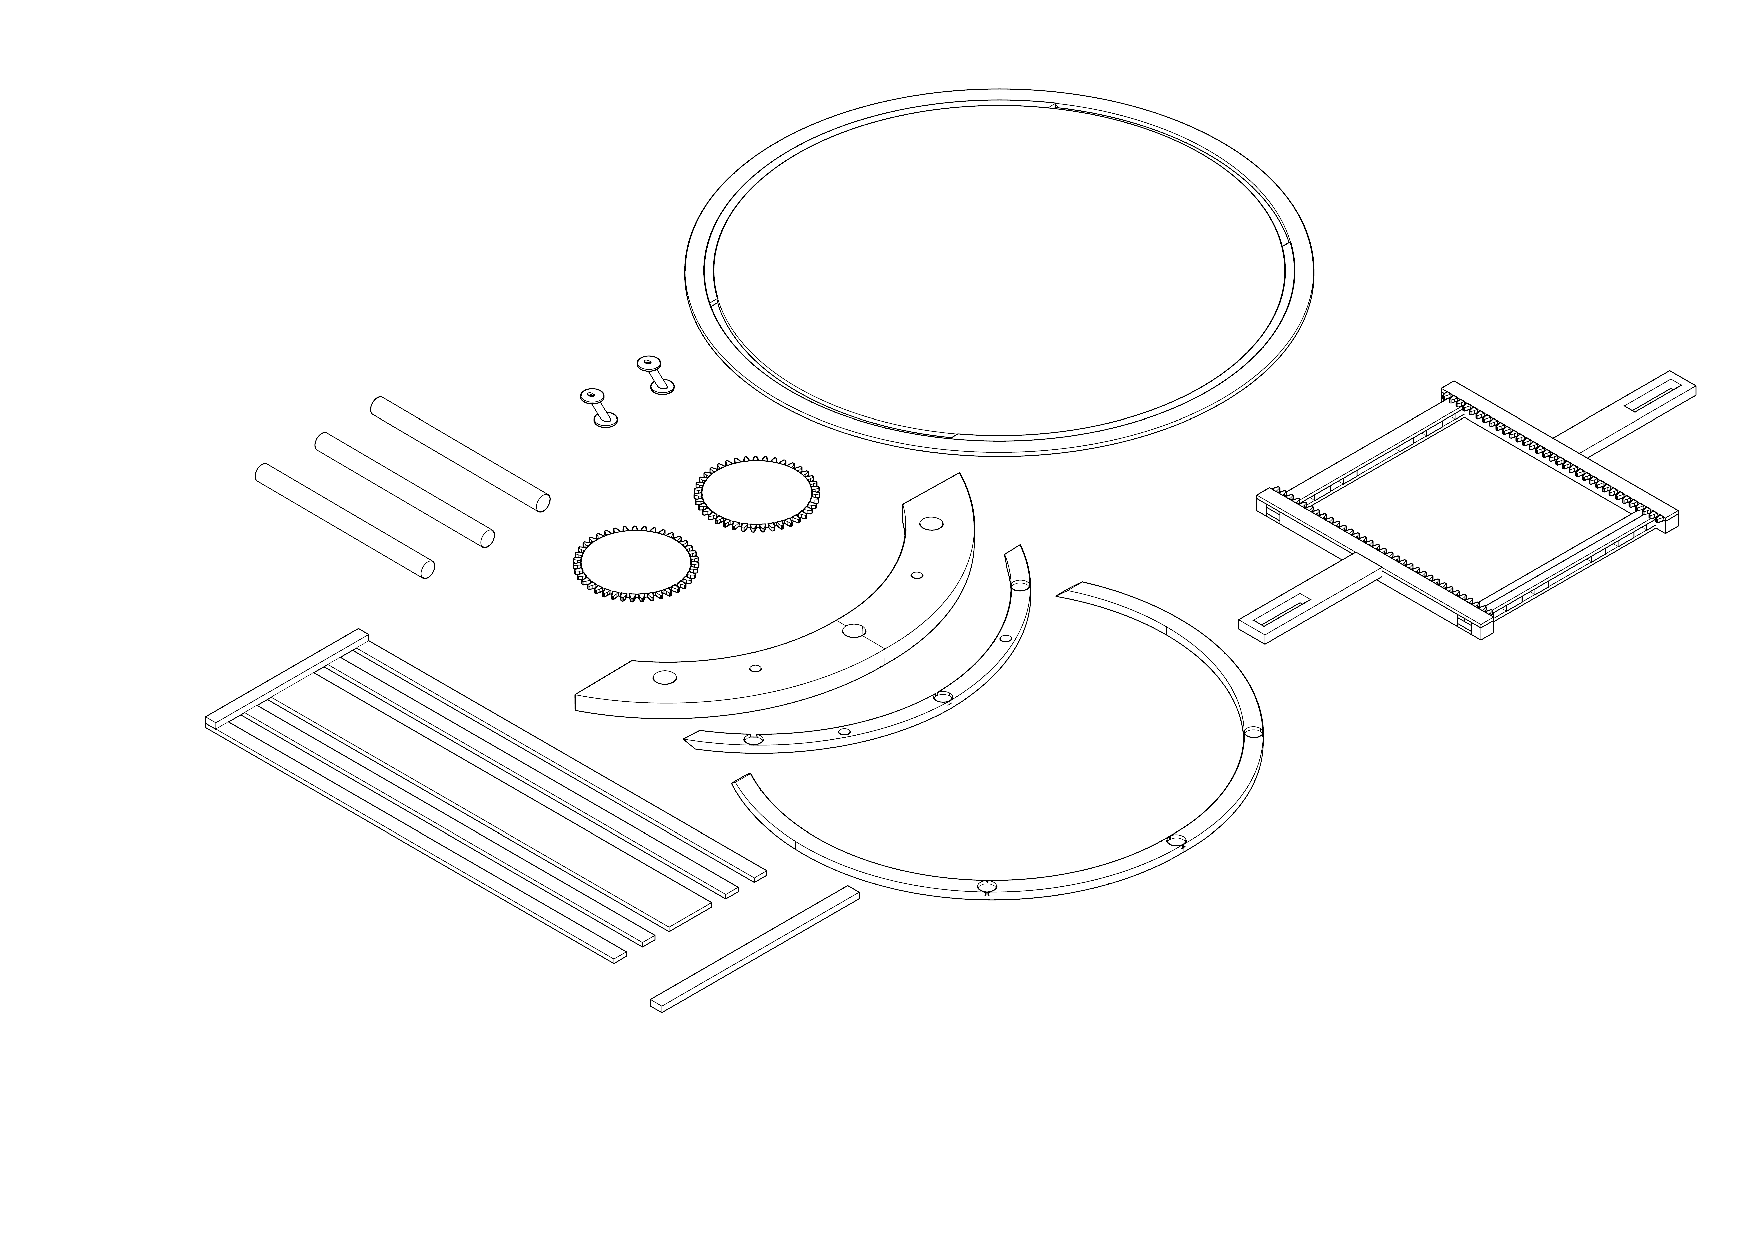
\includegraphics[width=.85\linewidth]{Images/ring prototype_v2 disect.pdf}
       \\{Individual Parts of the mechanic}
     
    \end{minipage}
    \captionof{figure}{CAD plans of the horizontal coordinate system prototype}
    \label{caddd}

\newpage


\subsection{The light approach}\label{light}
\begin{multicols}{2}
In parallel to the development of a potential mechanical setup, experimentations were made with using a LED light grid to display color coded information on the sun path. This poses three main questions. How should the grid of LEDS look like (shape, density, brightness, LED size, ...) and what does this grid have to do with the actual properties of the sun paths. Furthermore, how could a control system be implemented to manage LED color, state and brightness individually. These questions will be answered in the following sections.
\end{multicols}
\begin{multicols}{2}
[
\subsubsection{The shape of the grid and the role of the analemmas}
\label{ana}
]
    The installation's aesthetics were developed starting from the question of "How does the grid look like and how does it connect to the real sun path?". One of the key decisions was not to choose an equally spaced grid, but to represent the structures of the analemmas (cf. \textit{Section} \ref{anannn}). By not having an equally spaced grid, but a grid based on the positions at the 21st of every month one is able to show and explain the characteristic shape of the analemas to the visitor. Furthermore by choosing the day of the 21st in every month ensures that the solstices as well as the equinoxes are part of the grid (namely lowest, highest and middle positons on the analemma shape).\\
    In my opinion, it makes sense to base grid on the yearly change of position for a certain hour (analemma), as these shapes also provide a certain aesthetic expression, I personally associate with a sun path. In my opinion, this leads to a more desirable expression of the whole artefact than if realised with an equally spaced grid or the daily paths of the sun ("semicircles") as the base shape. 
    
    \subsubsection{Viewing the analemmas from the top}
    As the model is viewed from the top by the visitor, most of the analemmas will be viewed from a top perspective. This is especially true for the Singapore case. As the LED lights have to shine down onto the model for the purpose of shadow casting, an opaque housing, such as the one used in the beginning (cf. \textit{Figure} \ref{lieing}), is not a solution, as the LEDs will not be directly visible for the viewer. Therefore, the LEDs need to be made visible from the top view.
    \end{multicols}
    \begin{figure}[H]
        \centering
        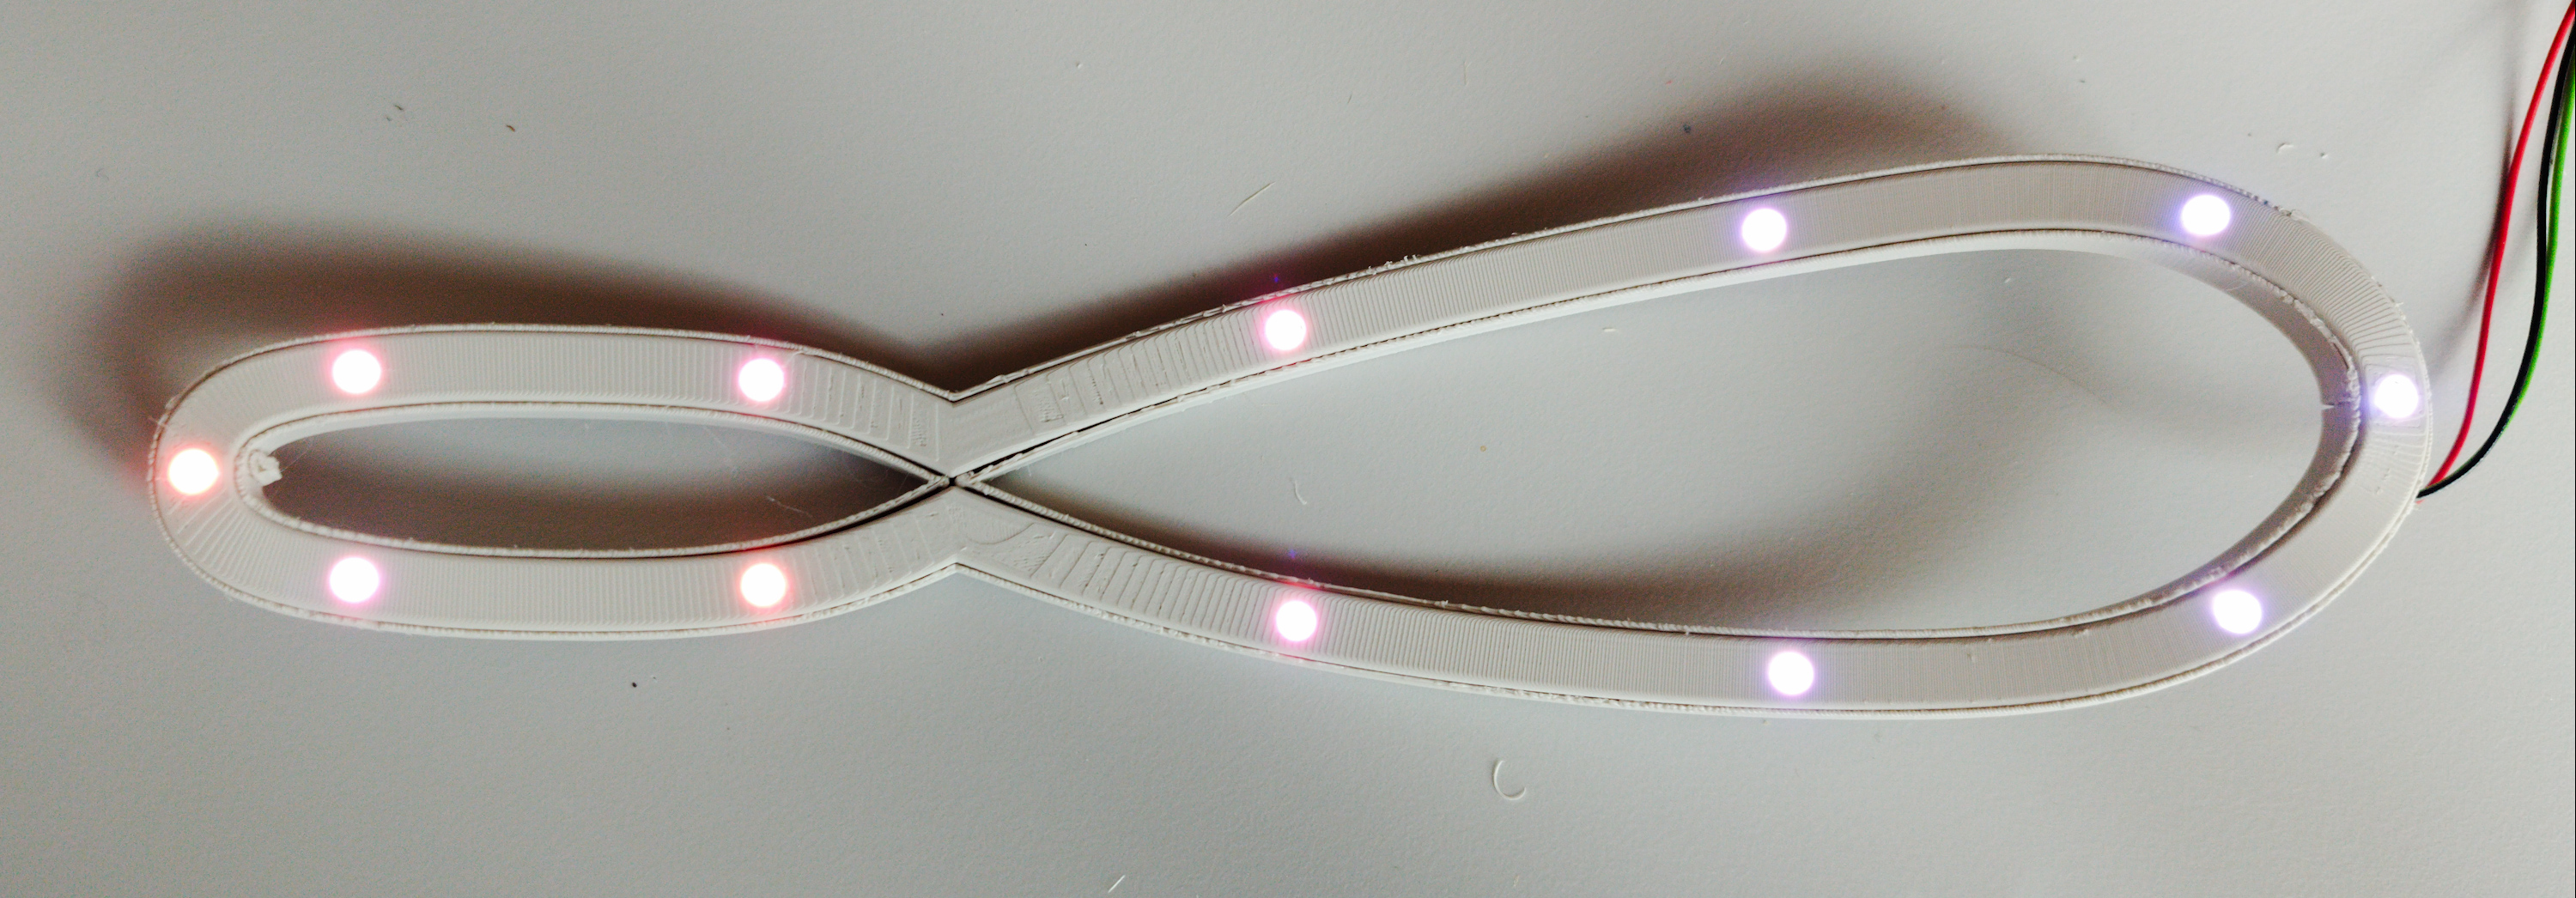
\includegraphics[width=0.85\linewidth]{Images/lig.jpg}
        \caption{First analemma prototype, opaque housing}
        \label{lieing}
    \end{figure}
    \begin{multicols}{2}
  
    To adress this problem, a certain transparency needs to be introduced into the housing of the LEDs. In that way the viewer can determine from the top view, which LEDs are active. Two options were tested, a fully transparent analemma (base and lid transparent) and a transparent analemma (base transparent, lid opaque) with a closed back. In the first one, the LED lights are clearly visible shining through to the back. In the second one it is more a small dim glow at the side. Therefore, the fully transparent analemma was chosen (cf. \textit{Figure} \ref{ligtt}).
    \end{multicols}
    \begin{figure}[H]
        \centering
        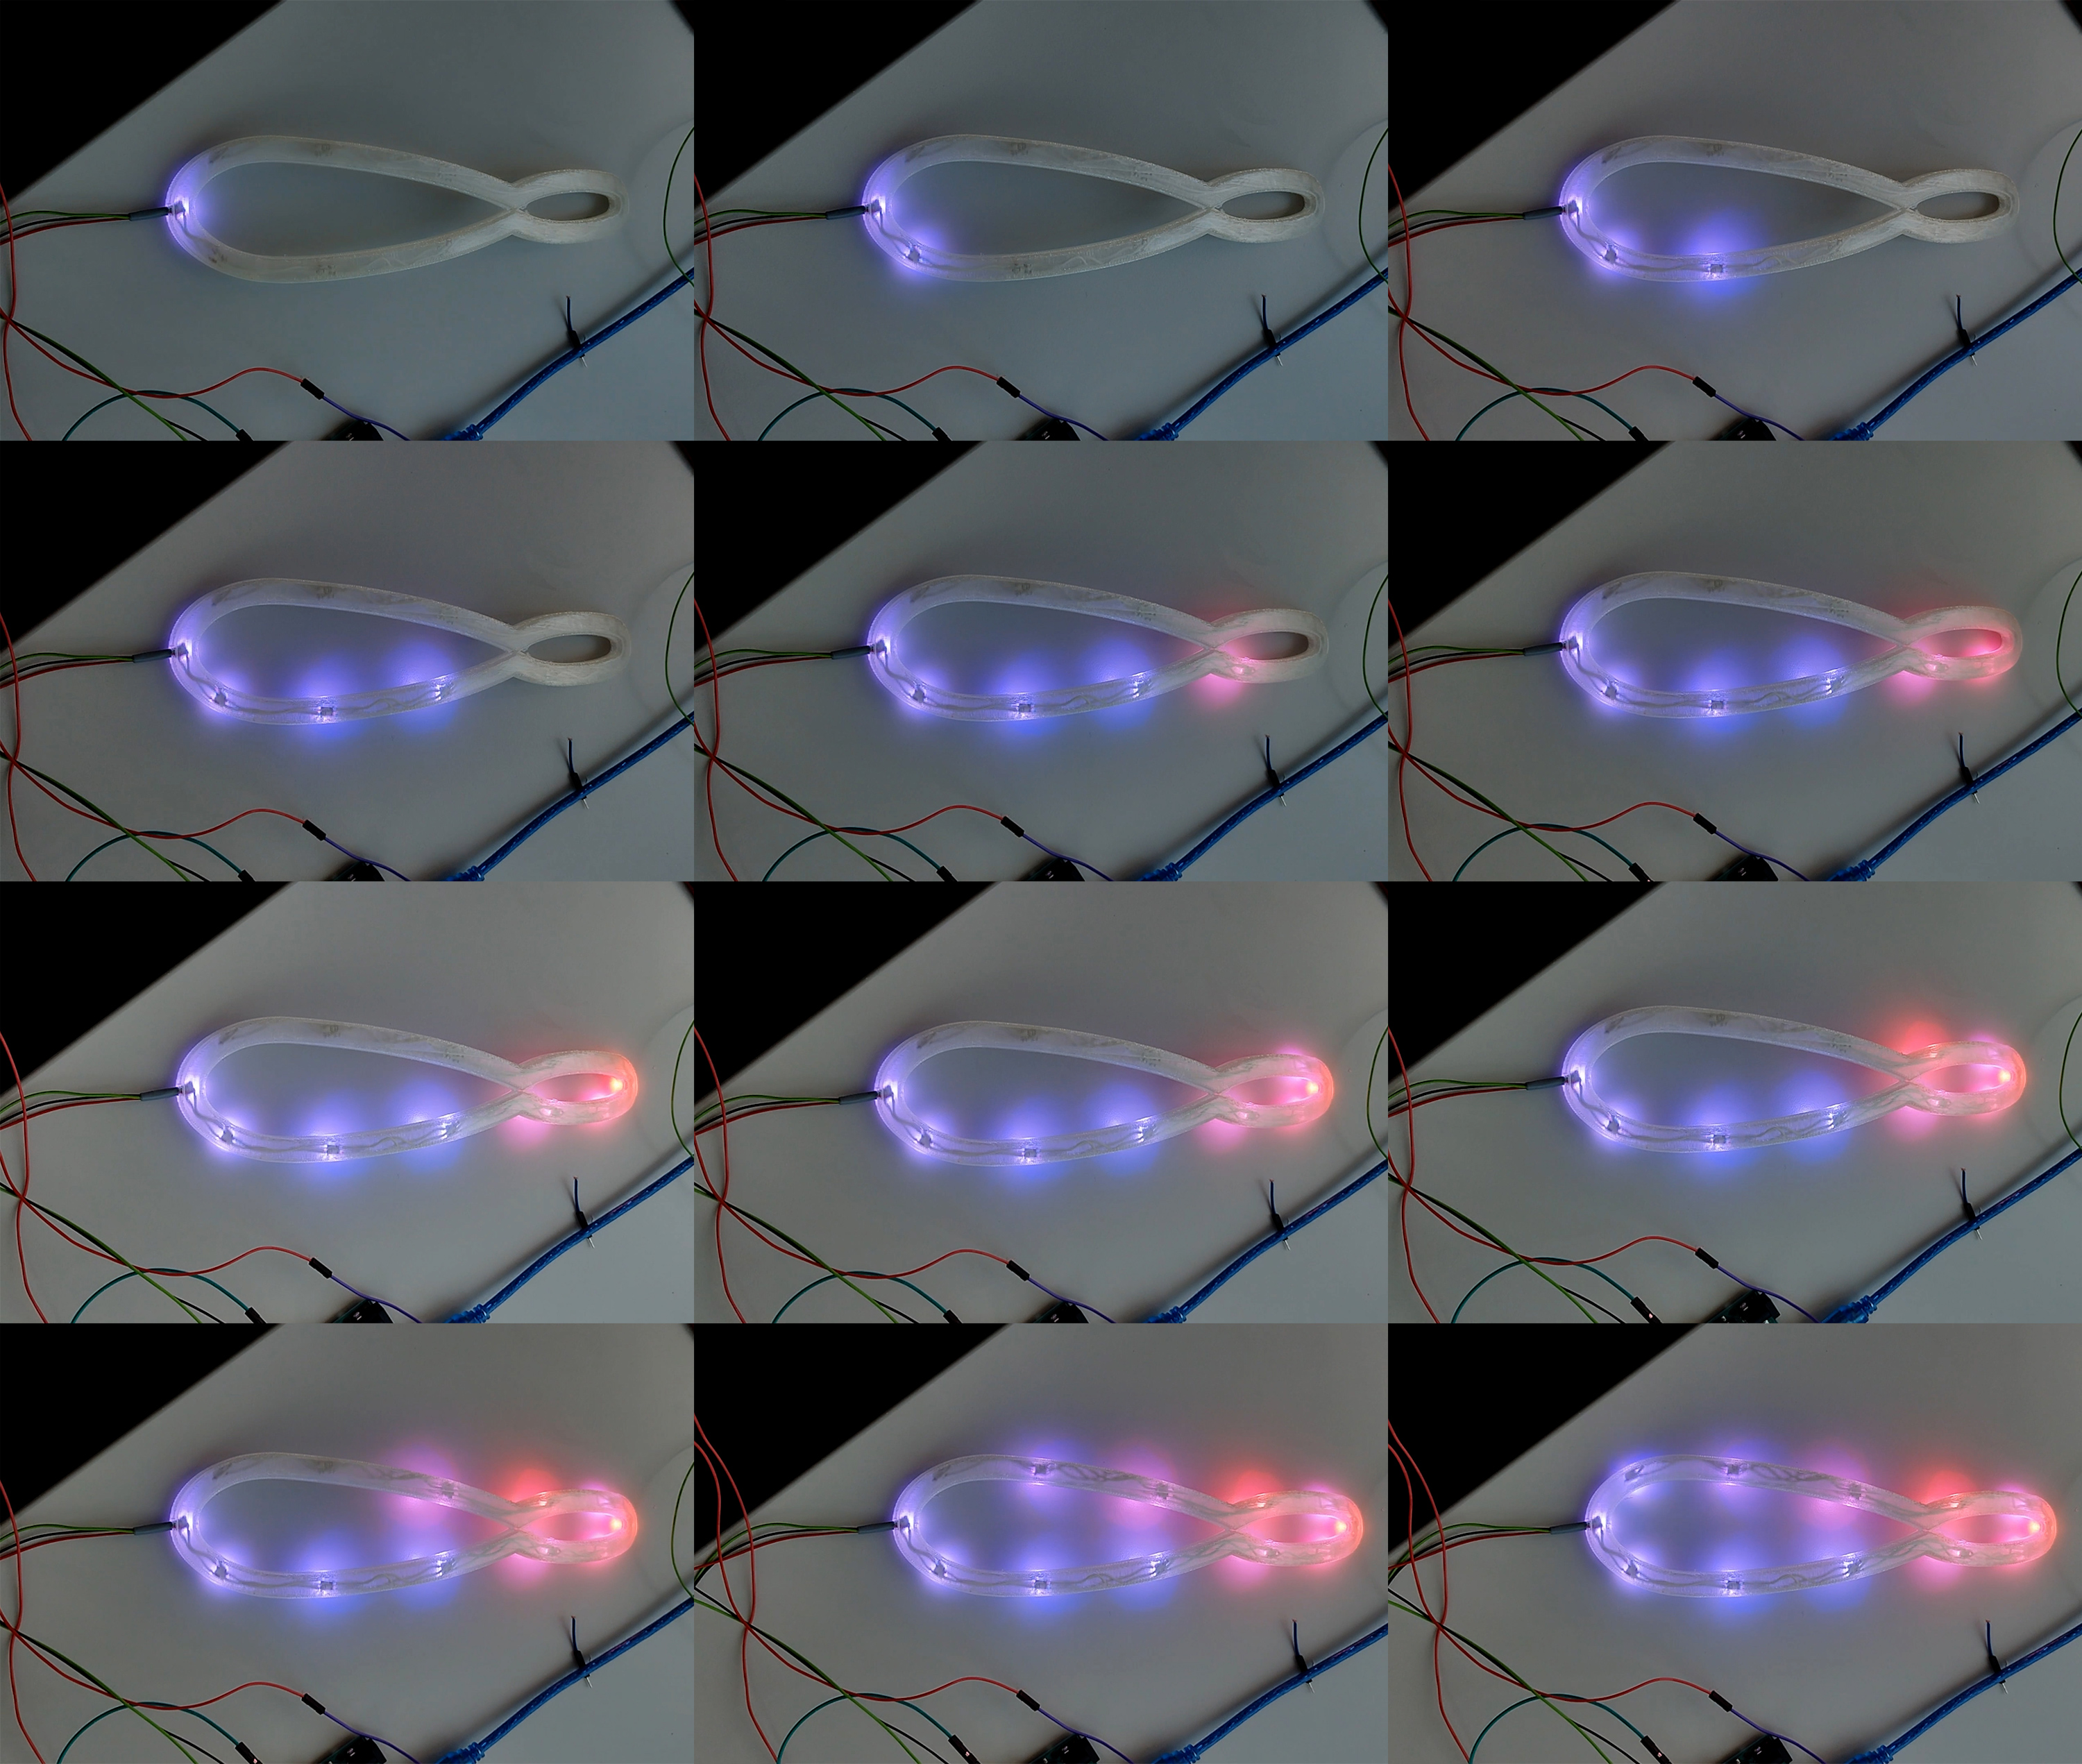
\includegraphics[width=.9\linewidth]{Images/lights.jpg}
        \caption{Glow of the LED lights through a fully transparent Analemma (base and lid)}
        \label{ligtt}
    \end{figure}
    \begin{multicols}{2}
    To improve the transparency of the 3D print, the number of top and bottom layers was reduced to 2 layers, such that the printed surfaces are as thin as possible. Furthermore, by printing the analemmas standing on their side  (cf. \textit{Figure} \ref{print}), a more optimal layer orientation can be achieved, such that the transparency is further improved (cf. \textit{Figure} \ref{comp}).
    \end{multicols}
    \begin{minipage}{0.48\linewidth}
        \centering
        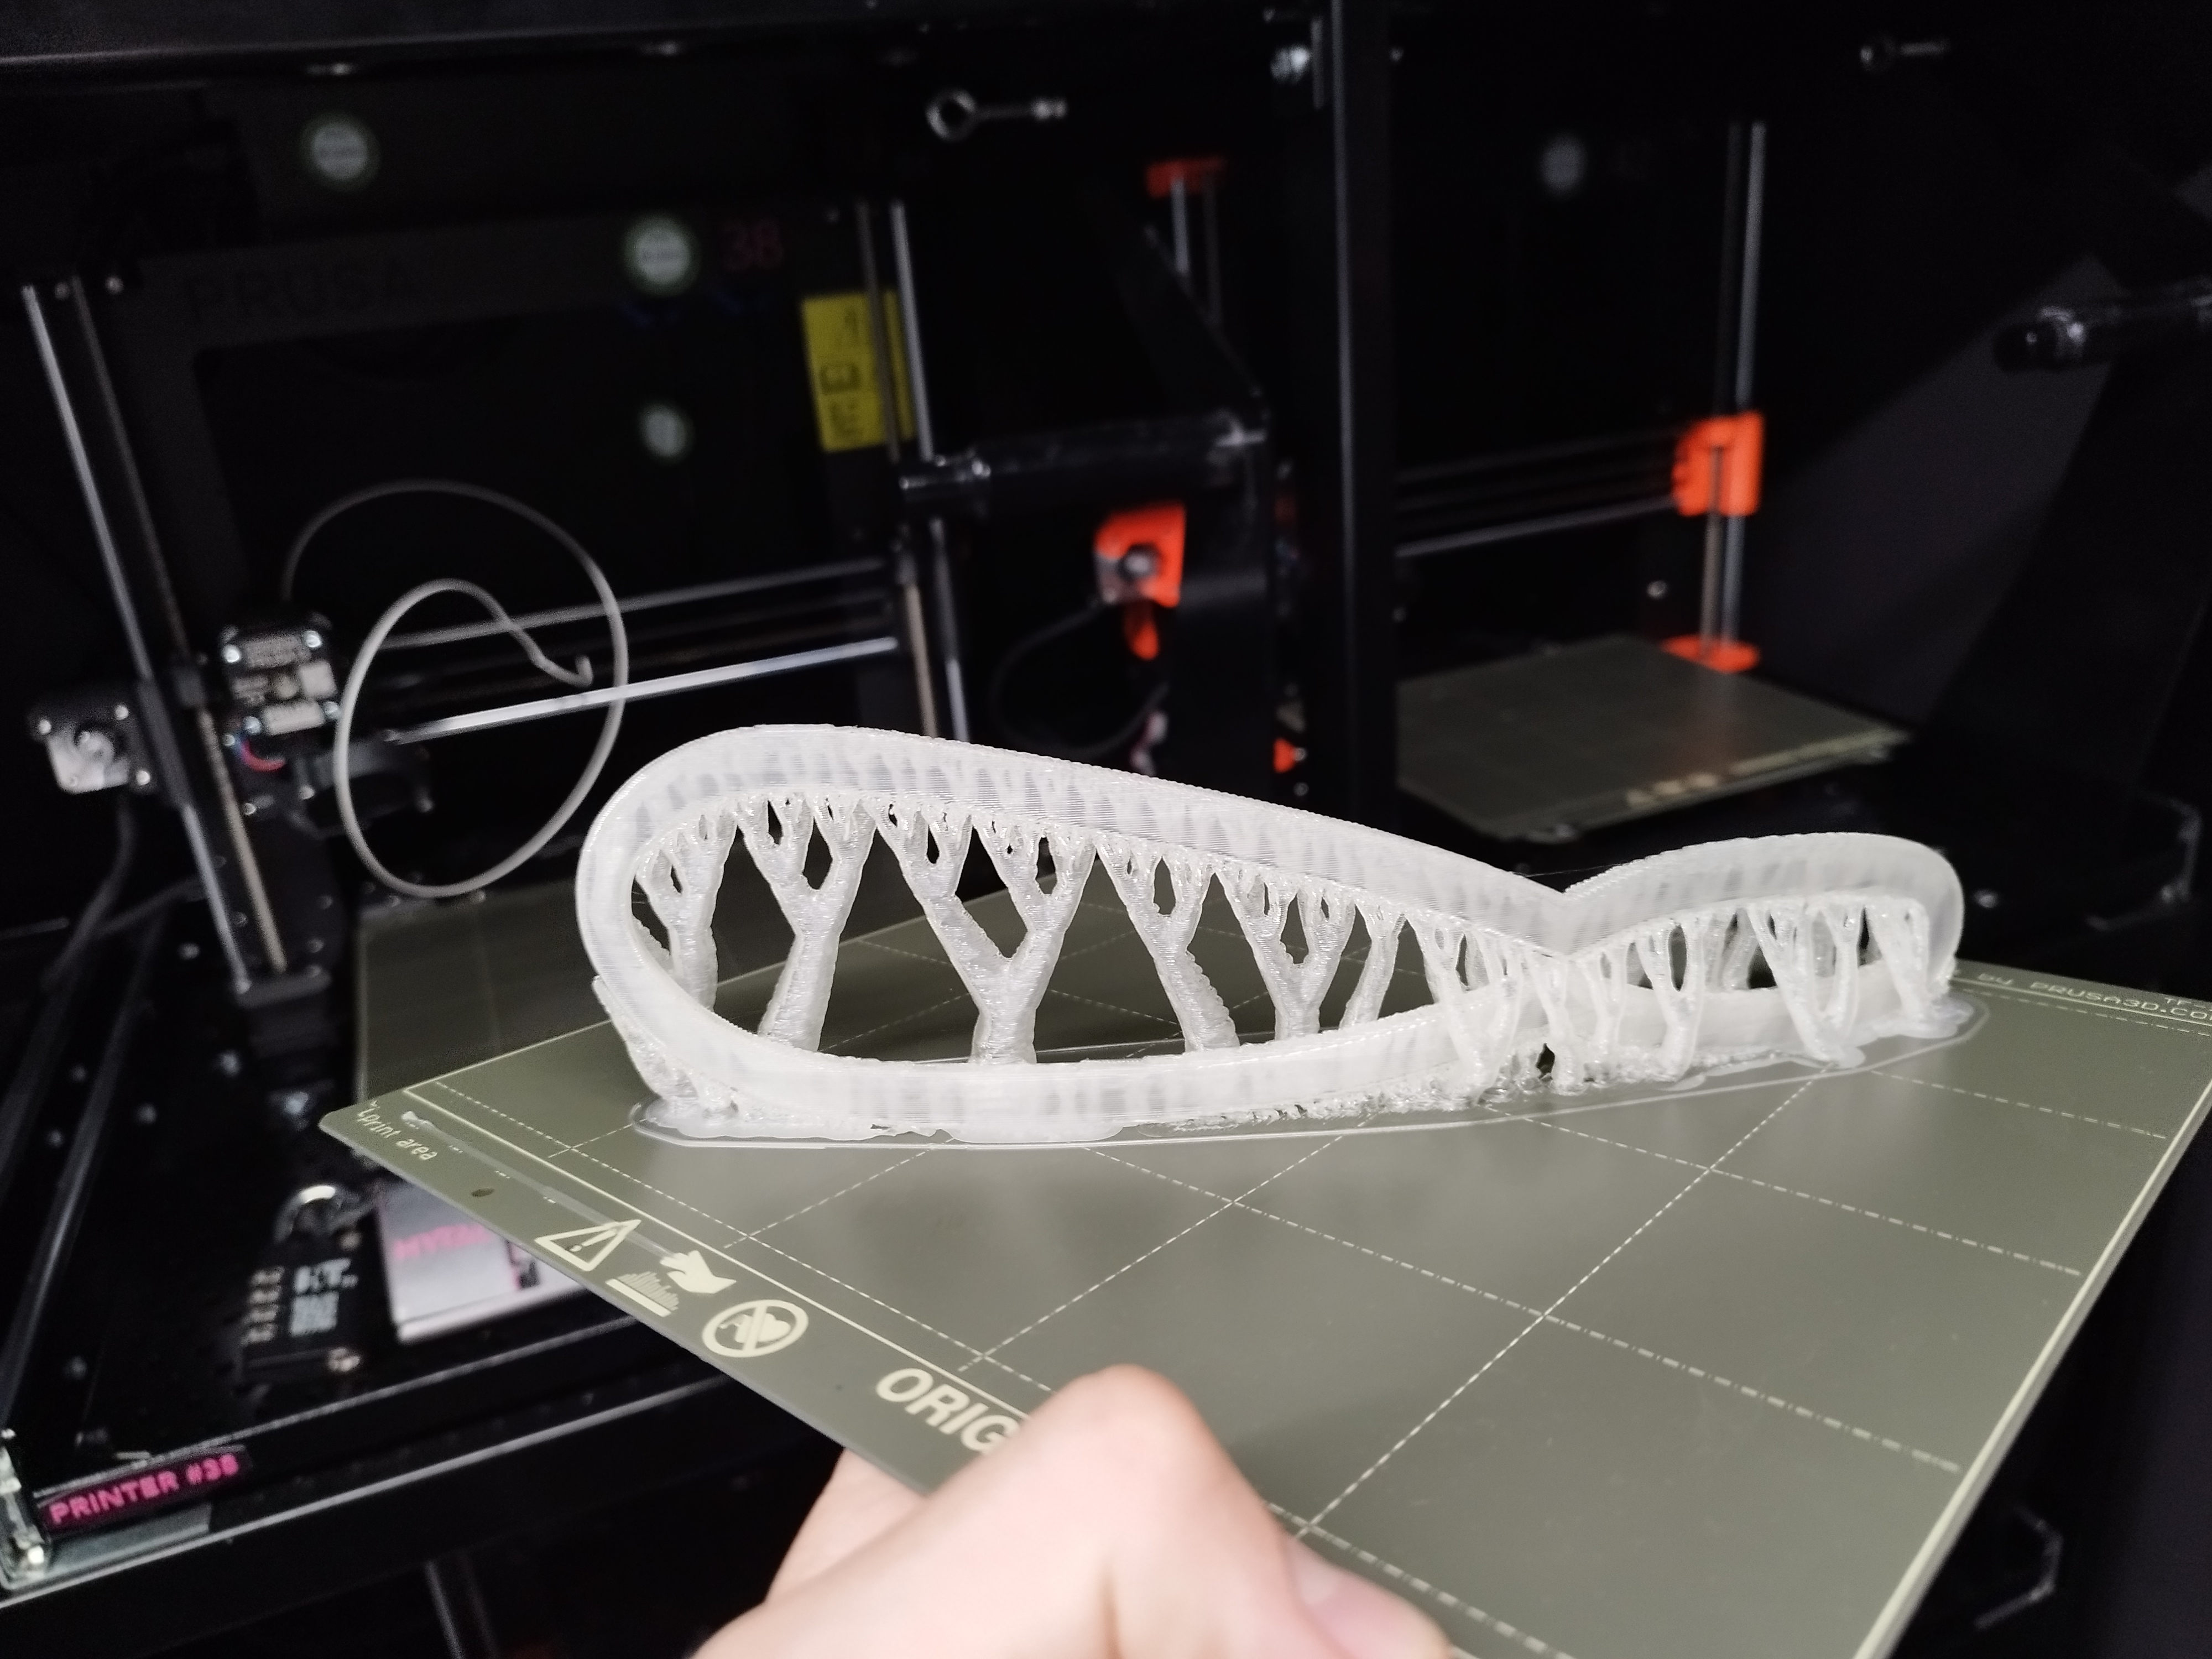
\includegraphics[width=.85\linewidth]{Images/p1.jpg}
        \\{front view}
    \end{minipage}
    \hfill
    \begin{minipage}{0.48\linewidth}
         \centering
        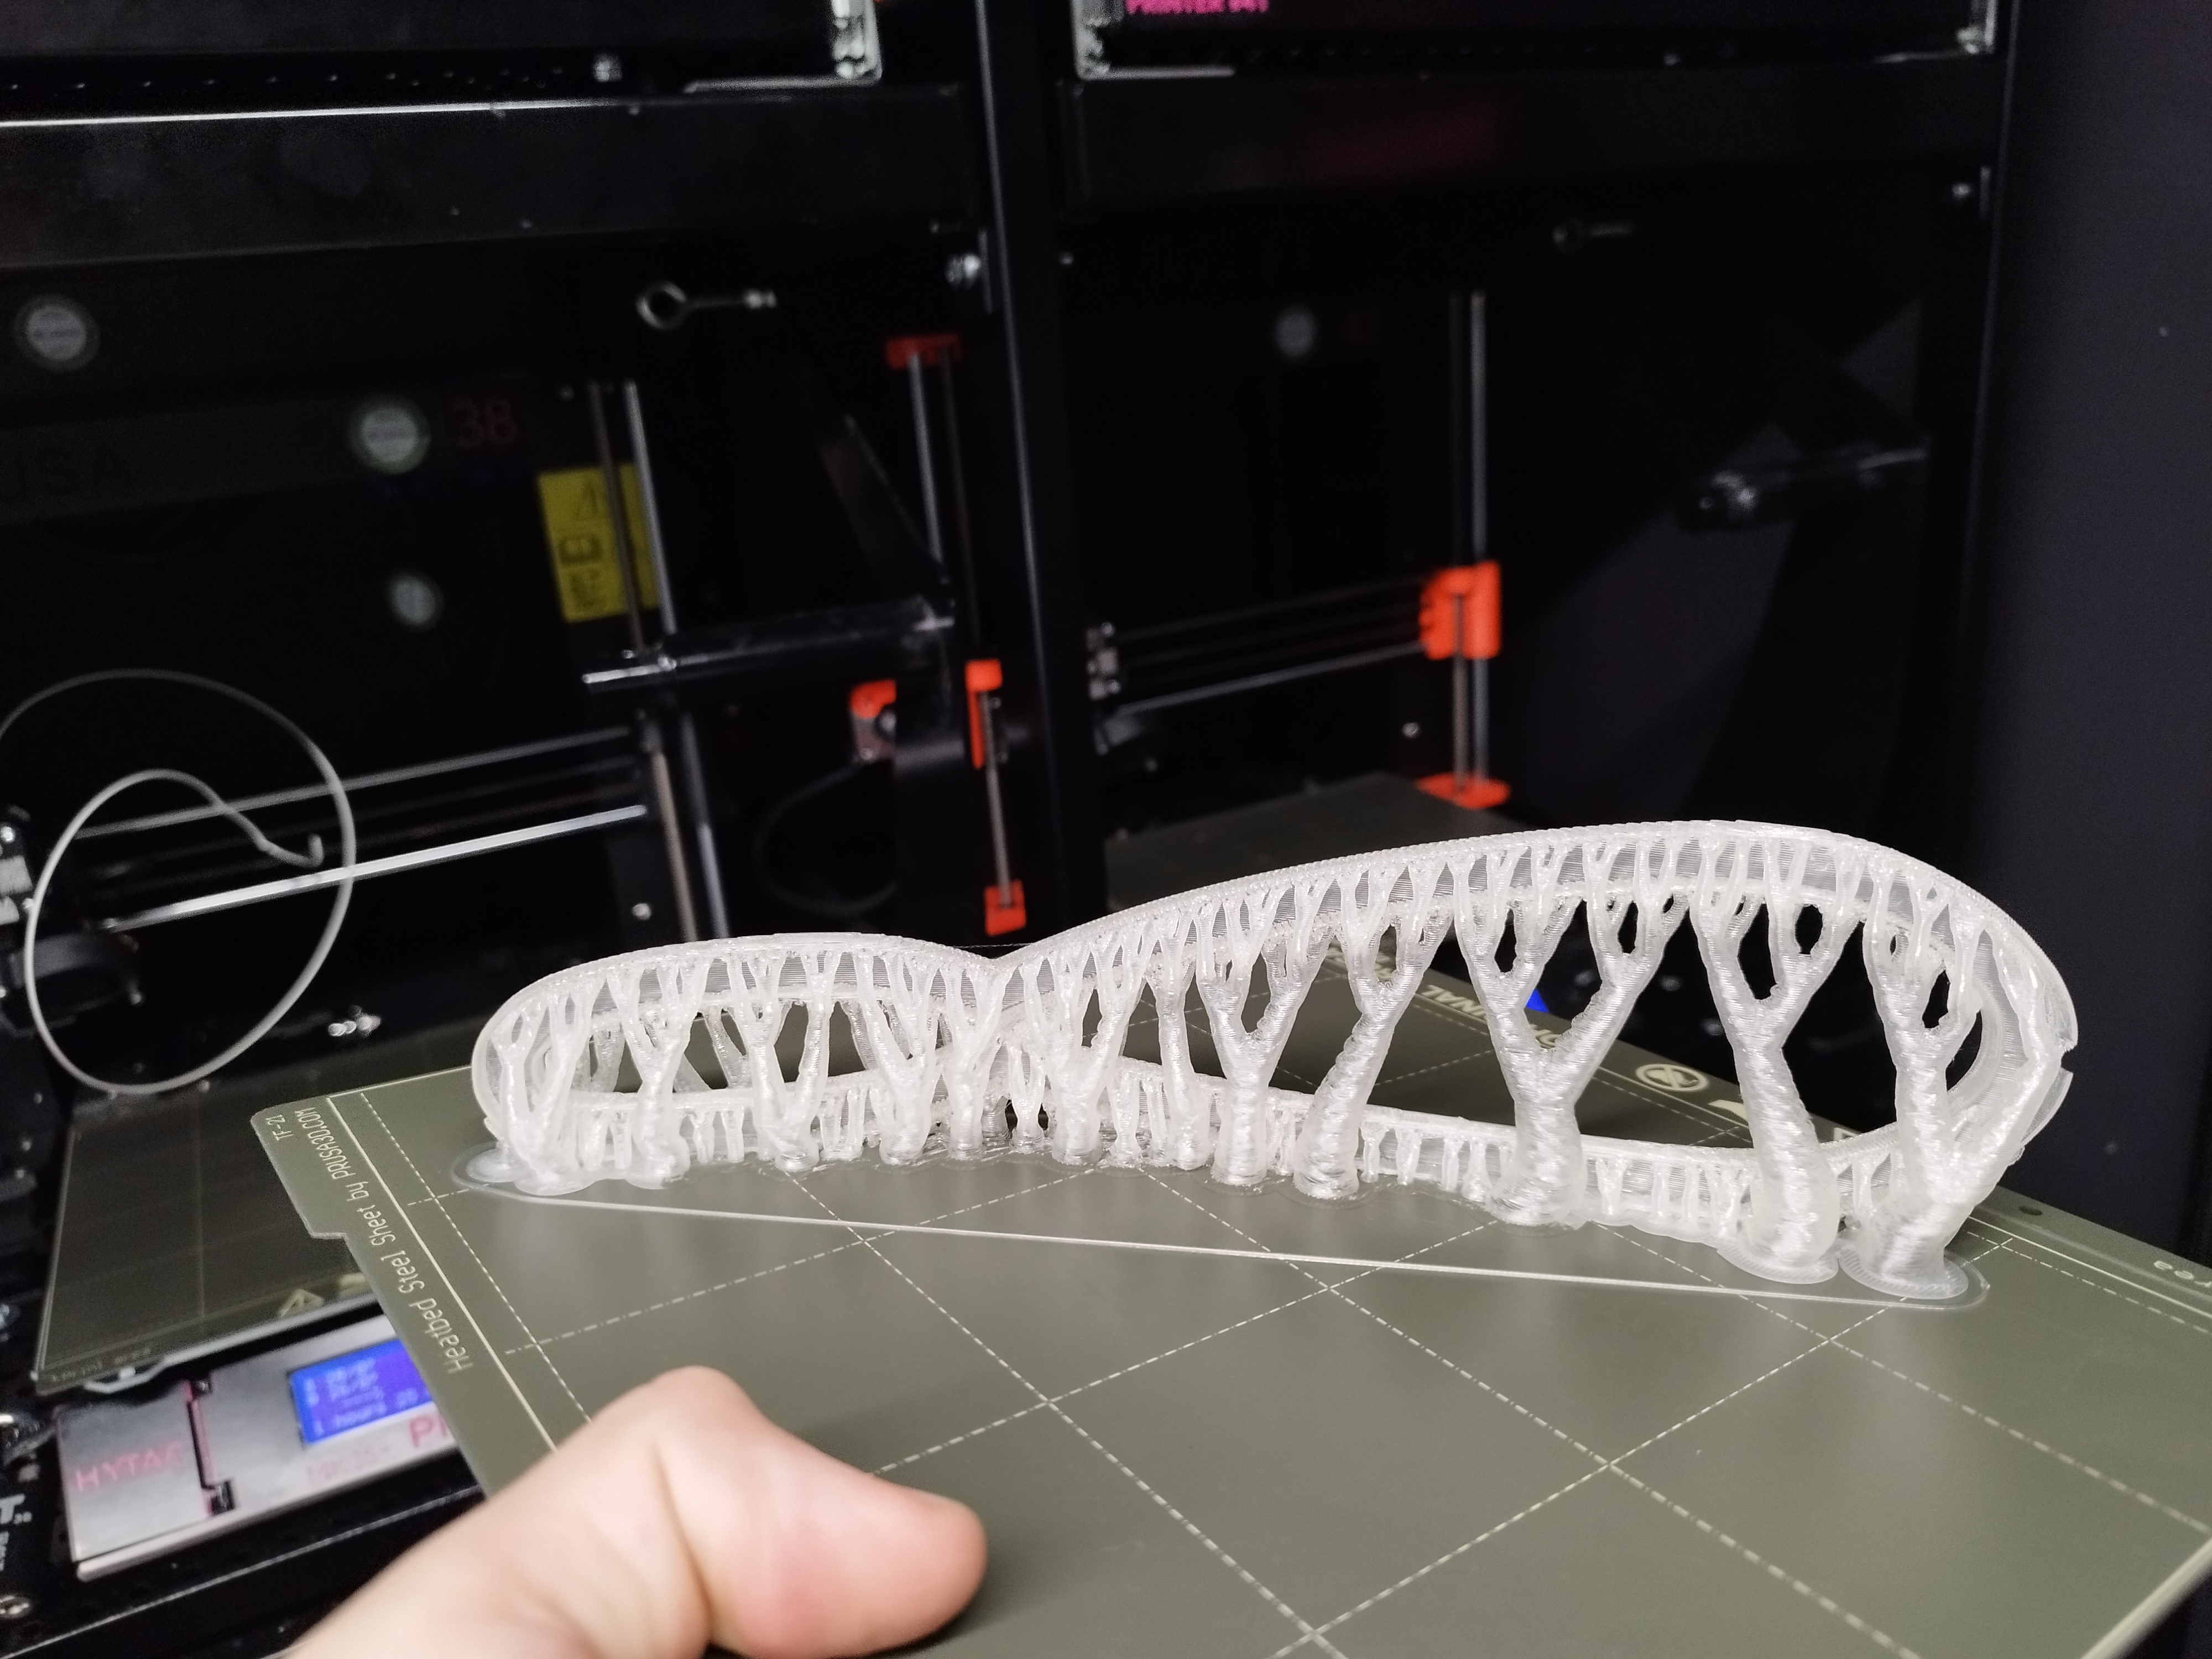
\includegraphics[width=.85\linewidth]{Images/p2.jpg}
     \\{back view}
        
    \end{minipage}
    \captionof{figure}{3D printing in a standing position for a more optimal layer orientation and as a result higher shell transparency}
    \label{print}
    \begin{multicols}{2}
    The shape of the analemma was first modelled using a simple offset of the analemma curve retrieved from the ladybug simulation tool. This offset led to an analemma shape, which was not connected in the middle (cf. \textit{Figure} \ref{comp}). However, as the analemma normally is association with the figure eight, it made sense to rework the housing and change it to an offset of the curves along a sphere. This led to a housing with a very nice looking figure eight shape (cf. \textit{Section} \ref{sunpa}).\\
    \\
    After quite a large number of iterations the shape was finalized and the lid was in a state, where it had a perfect fit into the base and a good transparency. For pictures of the final version of the analemma see \textit{Section} \ref{sunpa}.
\end{multicols}

\begin{minipage}{0.48\linewidth}
        \centering
        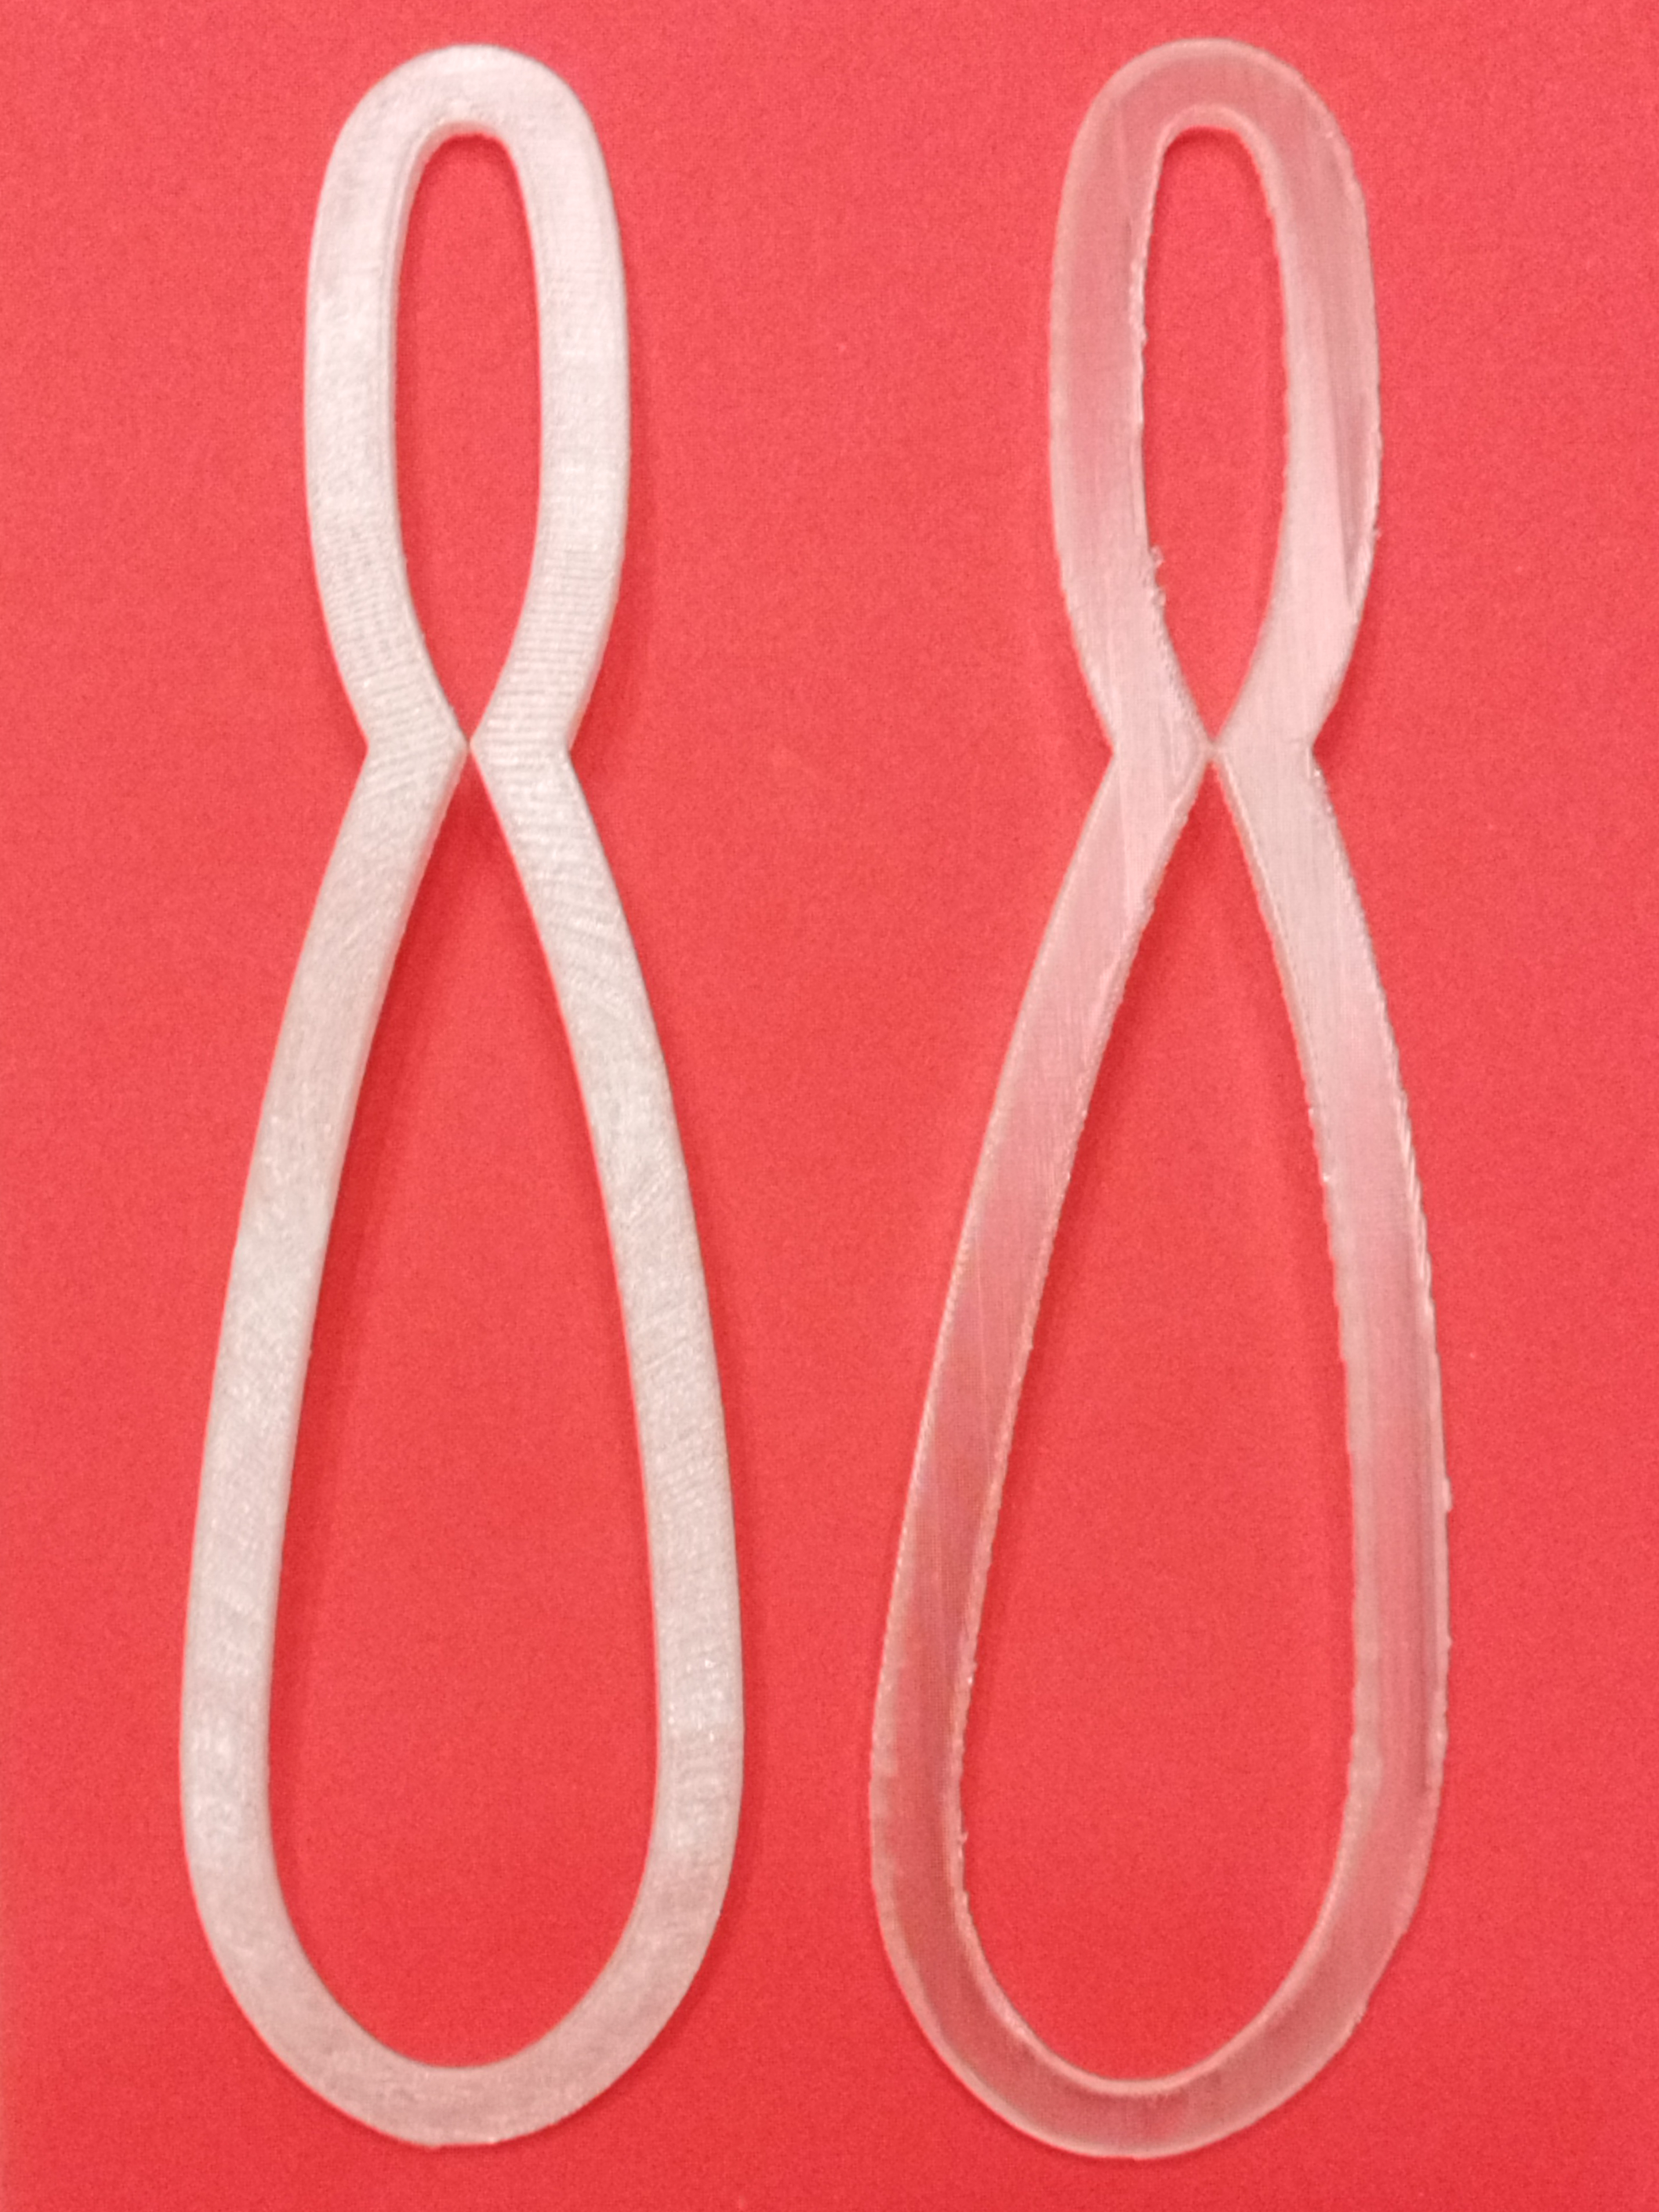
\includegraphics[width=.95\linewidth]{Images/t1.jpg}
        \\{lid}
            \end{minipage}
    \hfill
    \begin{minipage}{0.48\linewidth}
         \centering
        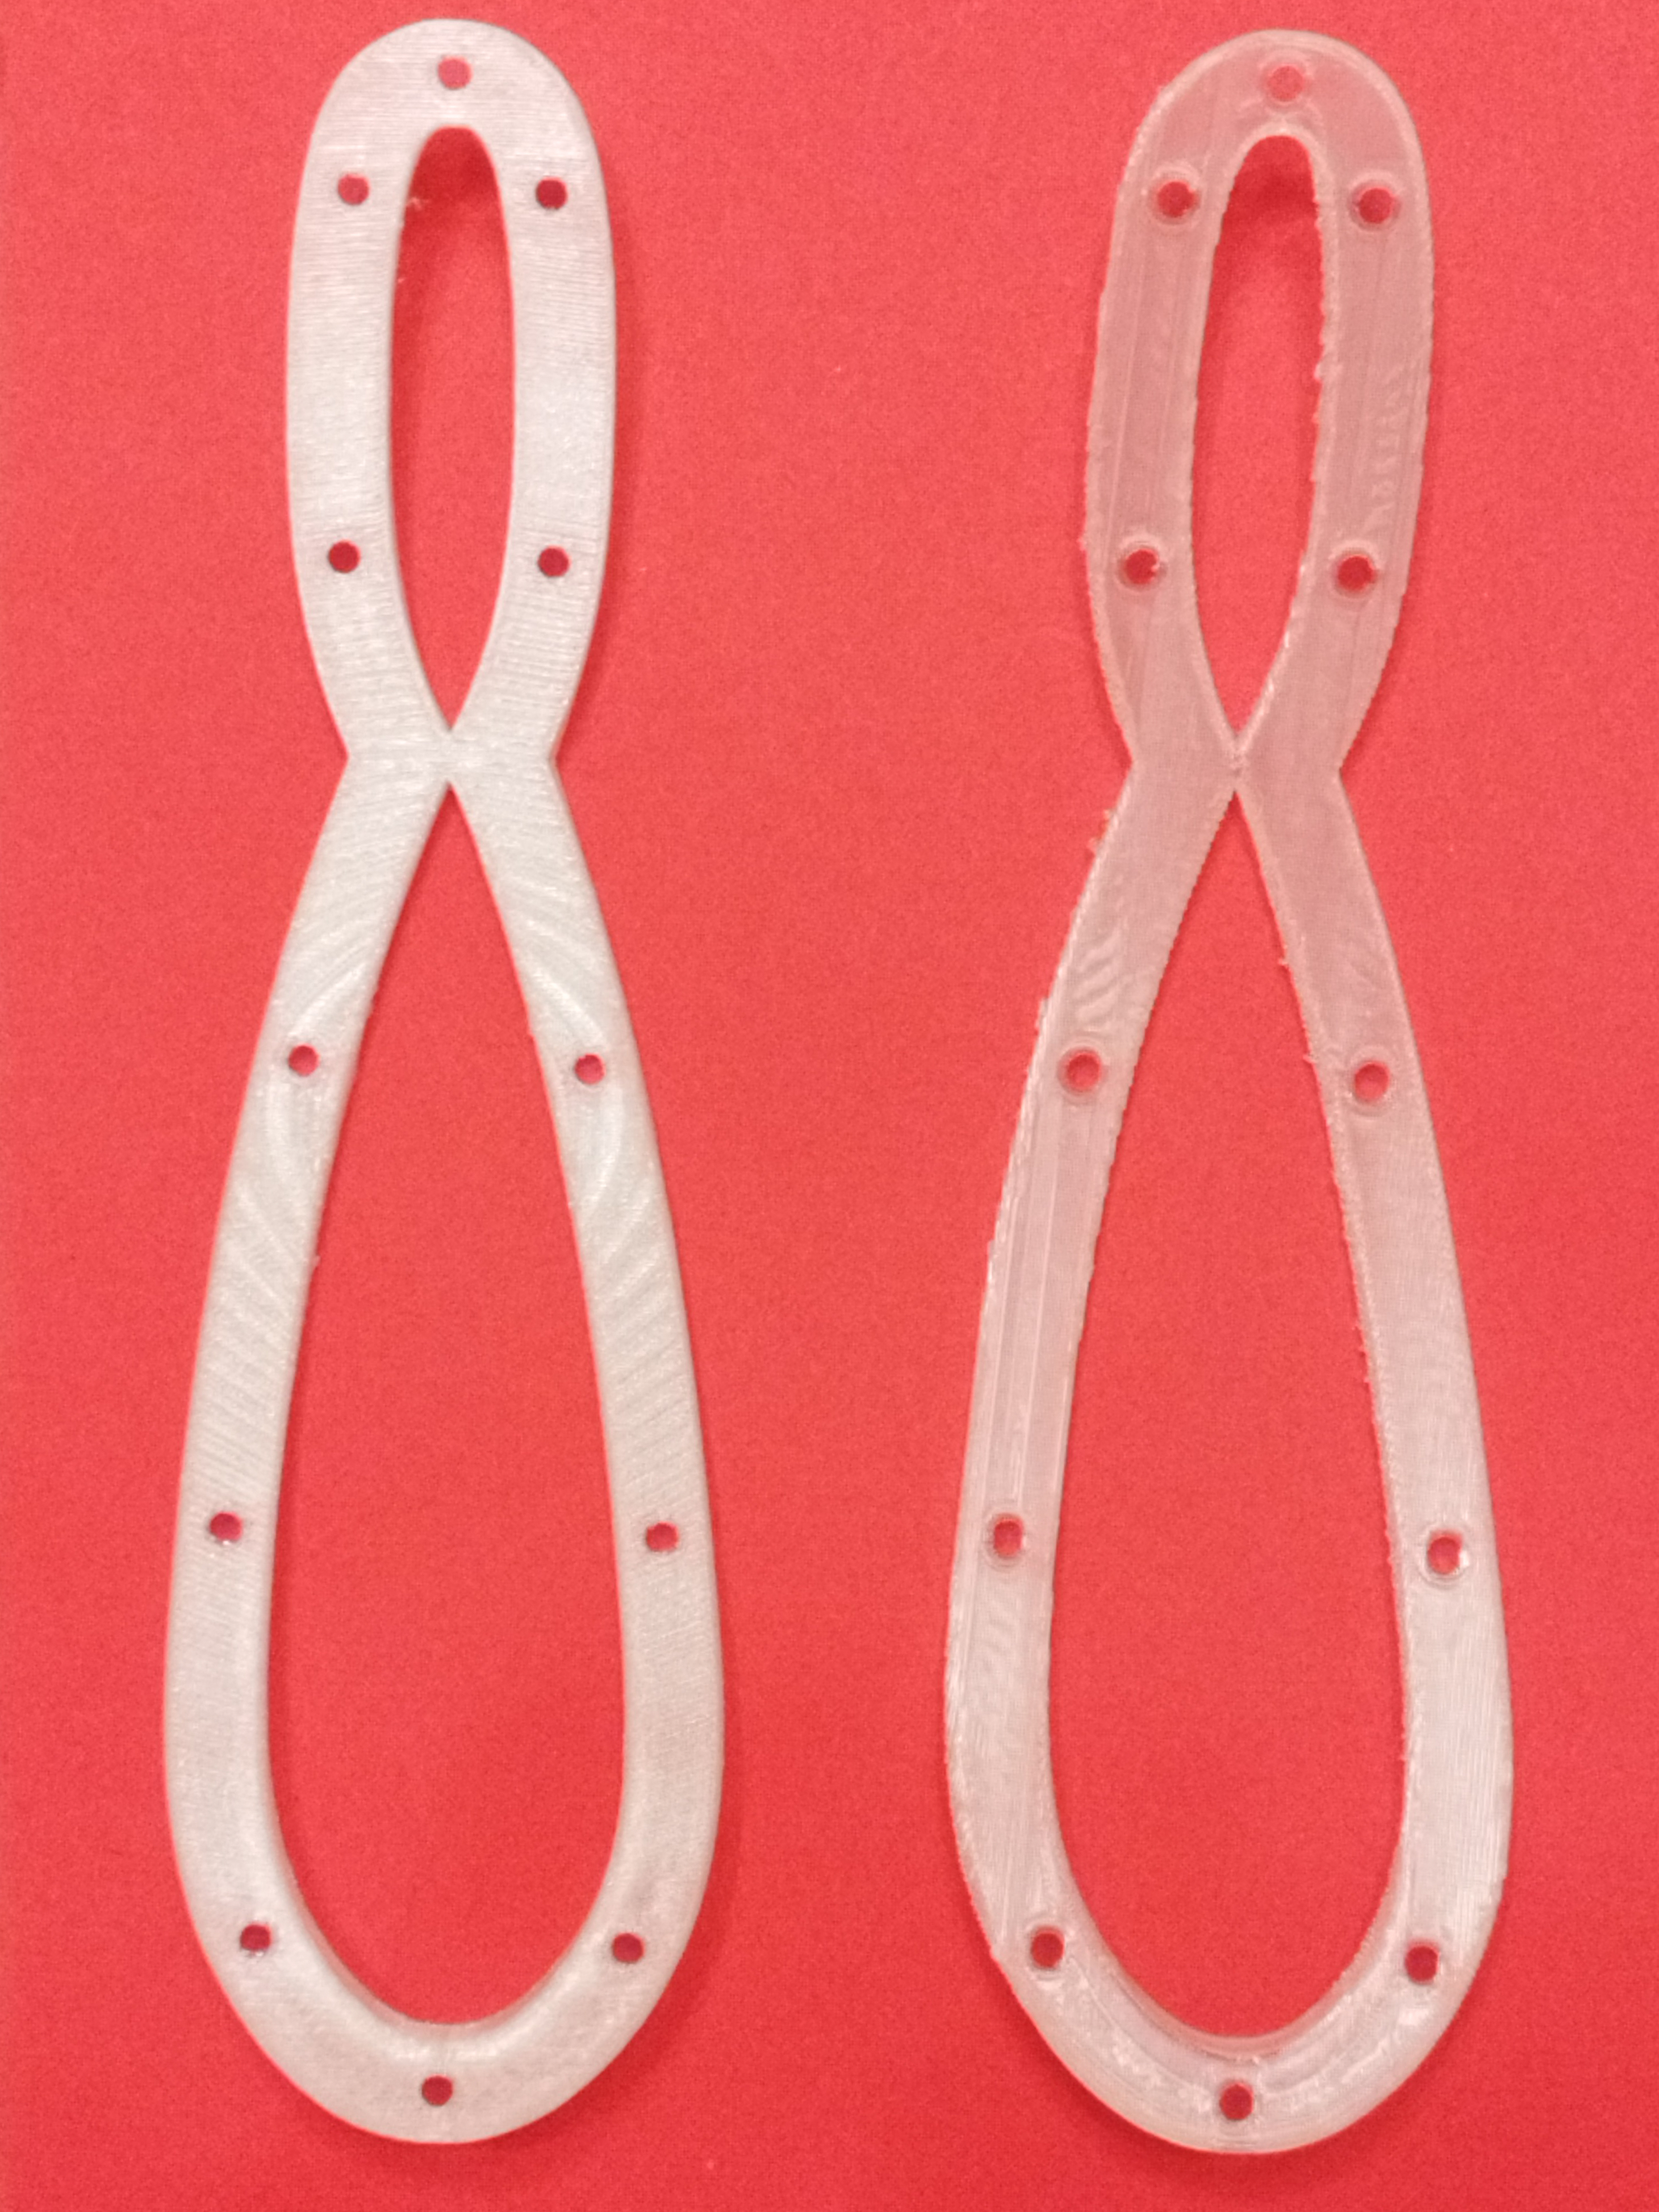
\includegraphics[width=.95\linewidth]{Images/t2.jpg}
     \\{base}
        
    \end{minipage}
    \captionof{figure}{Influence of printing orientation on transparency Left: lying printing orientation Right: standing printing orientation}
    \label{comp}
\newpage
\begin{multicols}{2}
[
 \subsubsection{Controlling the LEDs}
 ]
    To properly visualize information upon the sunpath model, it is necessary to control each LEDs color, state and brightness individually and simultaneously. The chosen representation of the sun path boast approximately 140 LED lights. For that reason an approach, where the lights are steered individually (meaning that every LED would need a pin of the Arduino to be controlled), or in a Matrix (meaning that every row and every column needs a pin) is infeasible. The first solution is infeasible as the Arduino only has 54 digital pins and the second one has limitations, as not all combinations of LEDs being on and off are possible by controlling rows and columns (no independent control of the individual LEDs). Therefore a solution using a "LED chain" was chosen.\\
    \\
    The LED chain consists of LED lights which are all wired in parallel to the power source and controlled using a data wire connecting all of the LED lights (cf. \textit{Figure} \ref{LED chain diagram}). Meaning, that the control inputs and outputs of the individual LEDs are connected to a chain (cf. \textit{Figure} \ref{cabel}). The Arduino is used to send a signal to the first data input. The controller on the LED "cuts off" the first 32bits of control information and forwards the rest of the signal after amplification to the second LED, which takes the originally second 32bits (now the first 32bits in the forwarded data) as control input and so on. Using this technology, the whole chain of LEDs can be controlled with only one pin of the Arduino. The product chosen in our case is from "Intelligent LED Solutions" (ILPL-K501-RGBW-SK105-01 - SMD-LED) (cf. \textit{Figure} \ref{LED product}).
    \columnbreak
     \begin{figure}[H]
        \centering
        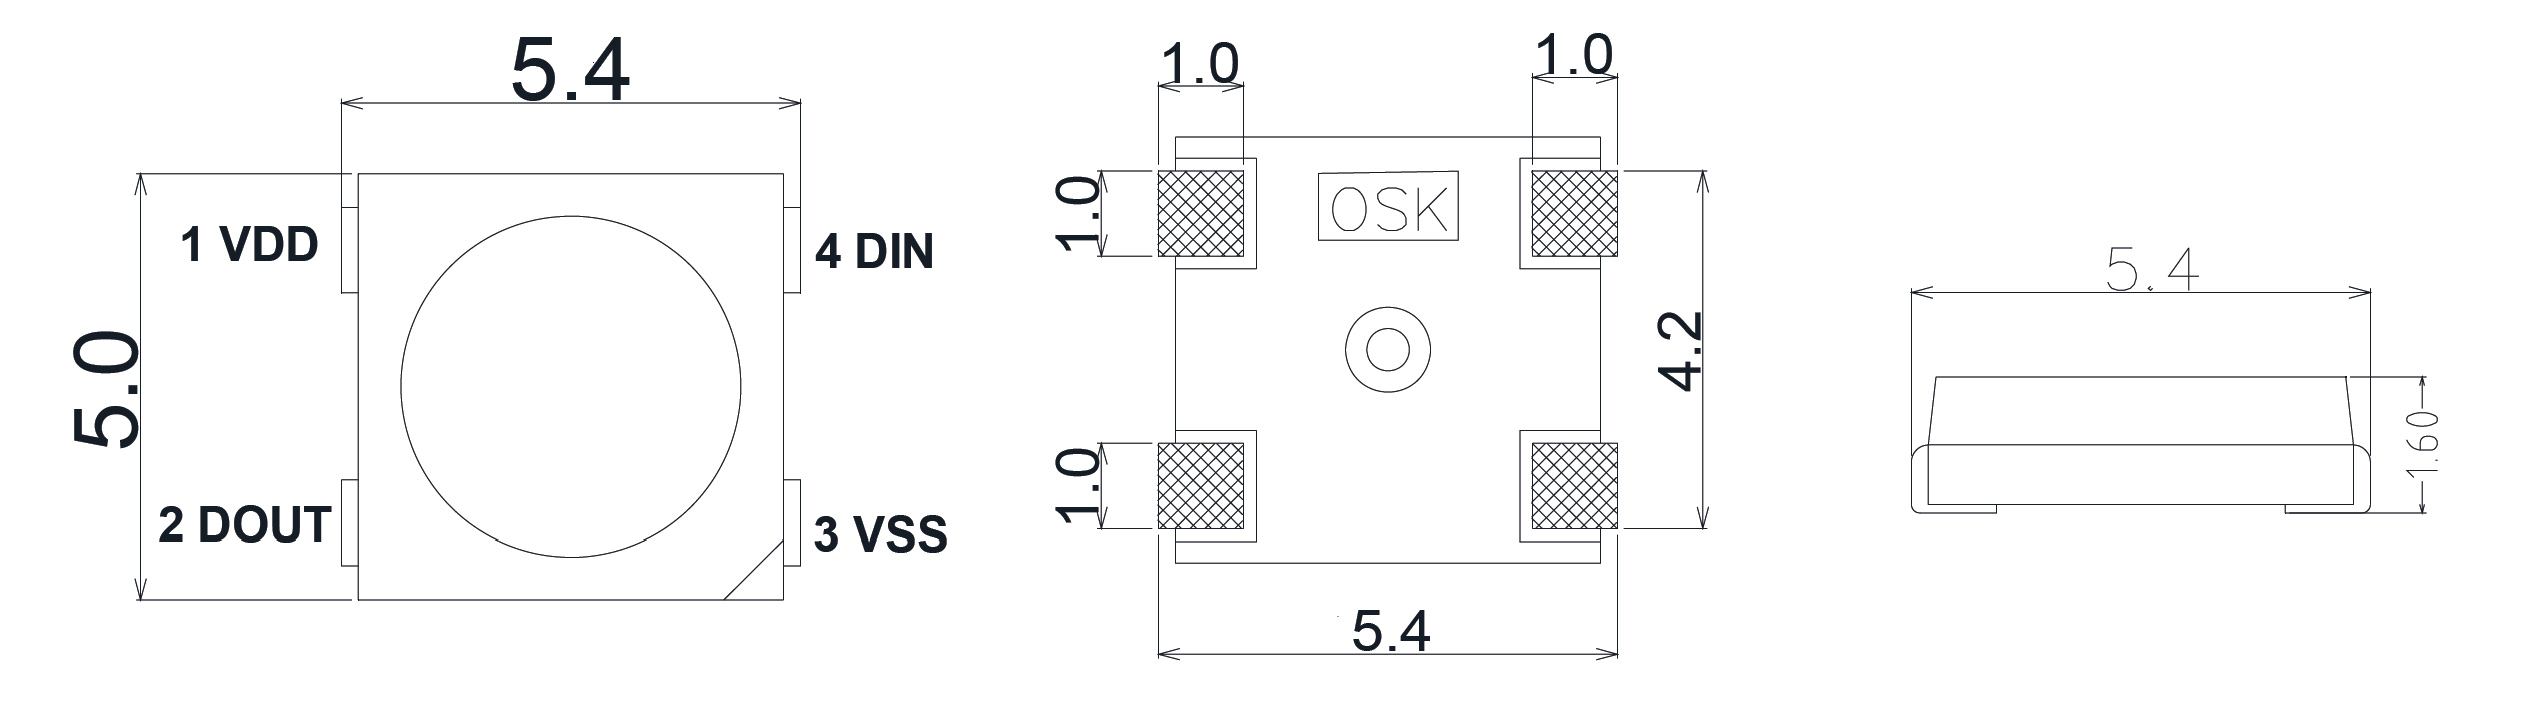
\includegraphics[width=0.7\linewidth]{Images/scheme led2_1.jpg}
        \captionof{figure}{Chosen Product from Intelligent LED Solutions \footnotemark}
        \label{LED product}
    \end{figure}
    \footnotetext{\footcite{inteli}}
    The LED's used are RGBW LEDs. This means that each of the LED units actually consists of 4 LED lights, one red, one green, one blue and one white. Thus, colors and brightness can be adjusted individually using an RGBW information of the scheme GBRW (cf. \textit{Figure} \ref{Signal}). This signal is transmitted using a frequency of 800khz and a transmission delay per LED of maximal 500ns.
     \begin{figure}[H]
        \centering
        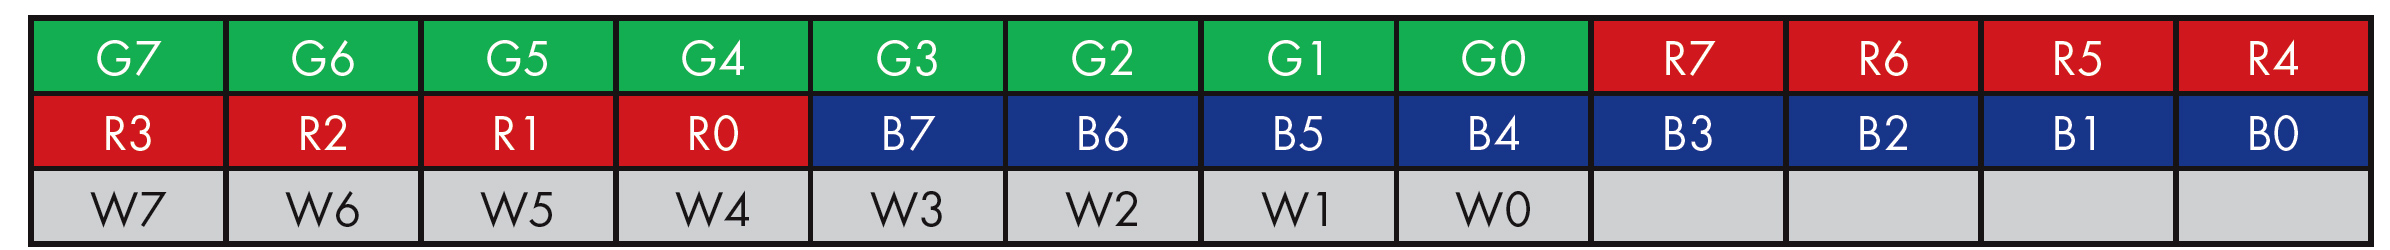
\includegraphics[width=0.7\linewidth]{Images/GRBW_1.jpg}
        \captionof{figure}{GRBW information scheme visualisation \footnotemark}
        \label{Signal}
    \end{figure}
    \footnotetext{\footcite{inteli}}
    The LEDs use the SK6812 standard for the data stream. The SK6812 control data was generated using the Neopixel library within the Arduino IDE. Using this standard allows for an easy programming of the LED lights without worrying about compatibility and the specific details about the components within the LED lights.

\end{multicols} 
\begin{minipage}{0.48\linewidth}
\begin{figure}[H]

        \centering
         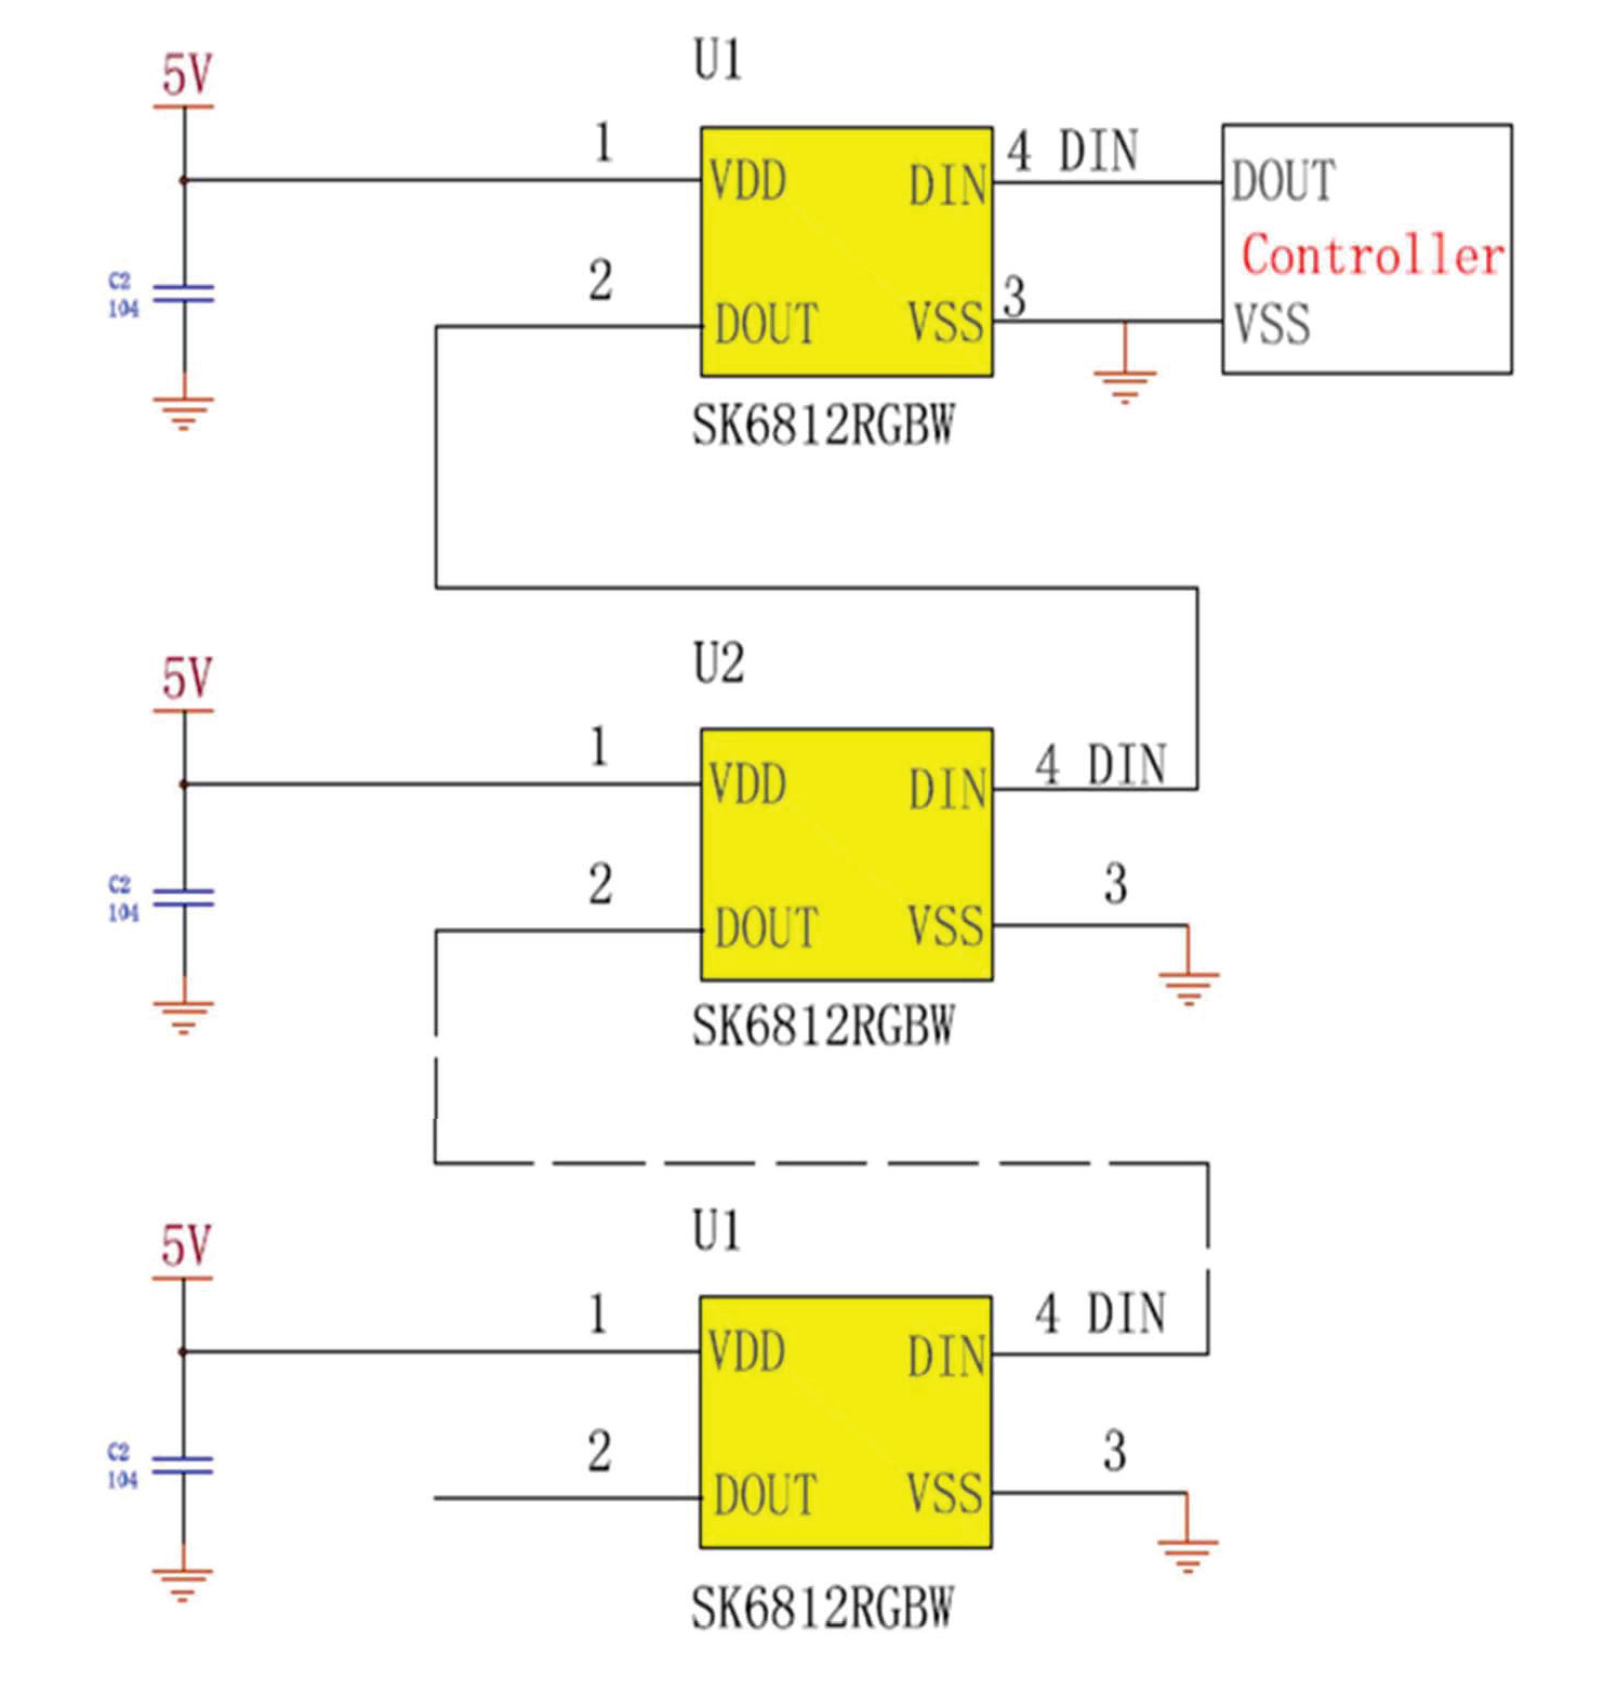
\includegraphics[width=.85\linewidth]{Images/chain_1.jpg}
       \captionof{figure}{Connection Scheme \footnotemark}
        \label{LED chain diagram}
    \end{figure}
    \end{minipage}
    \footnotetext{\footcite{inteli}}
    \hfill
    \begin{minipage}{0.48\linewidth}
    \begin{figure}[H]
   
         \centering
        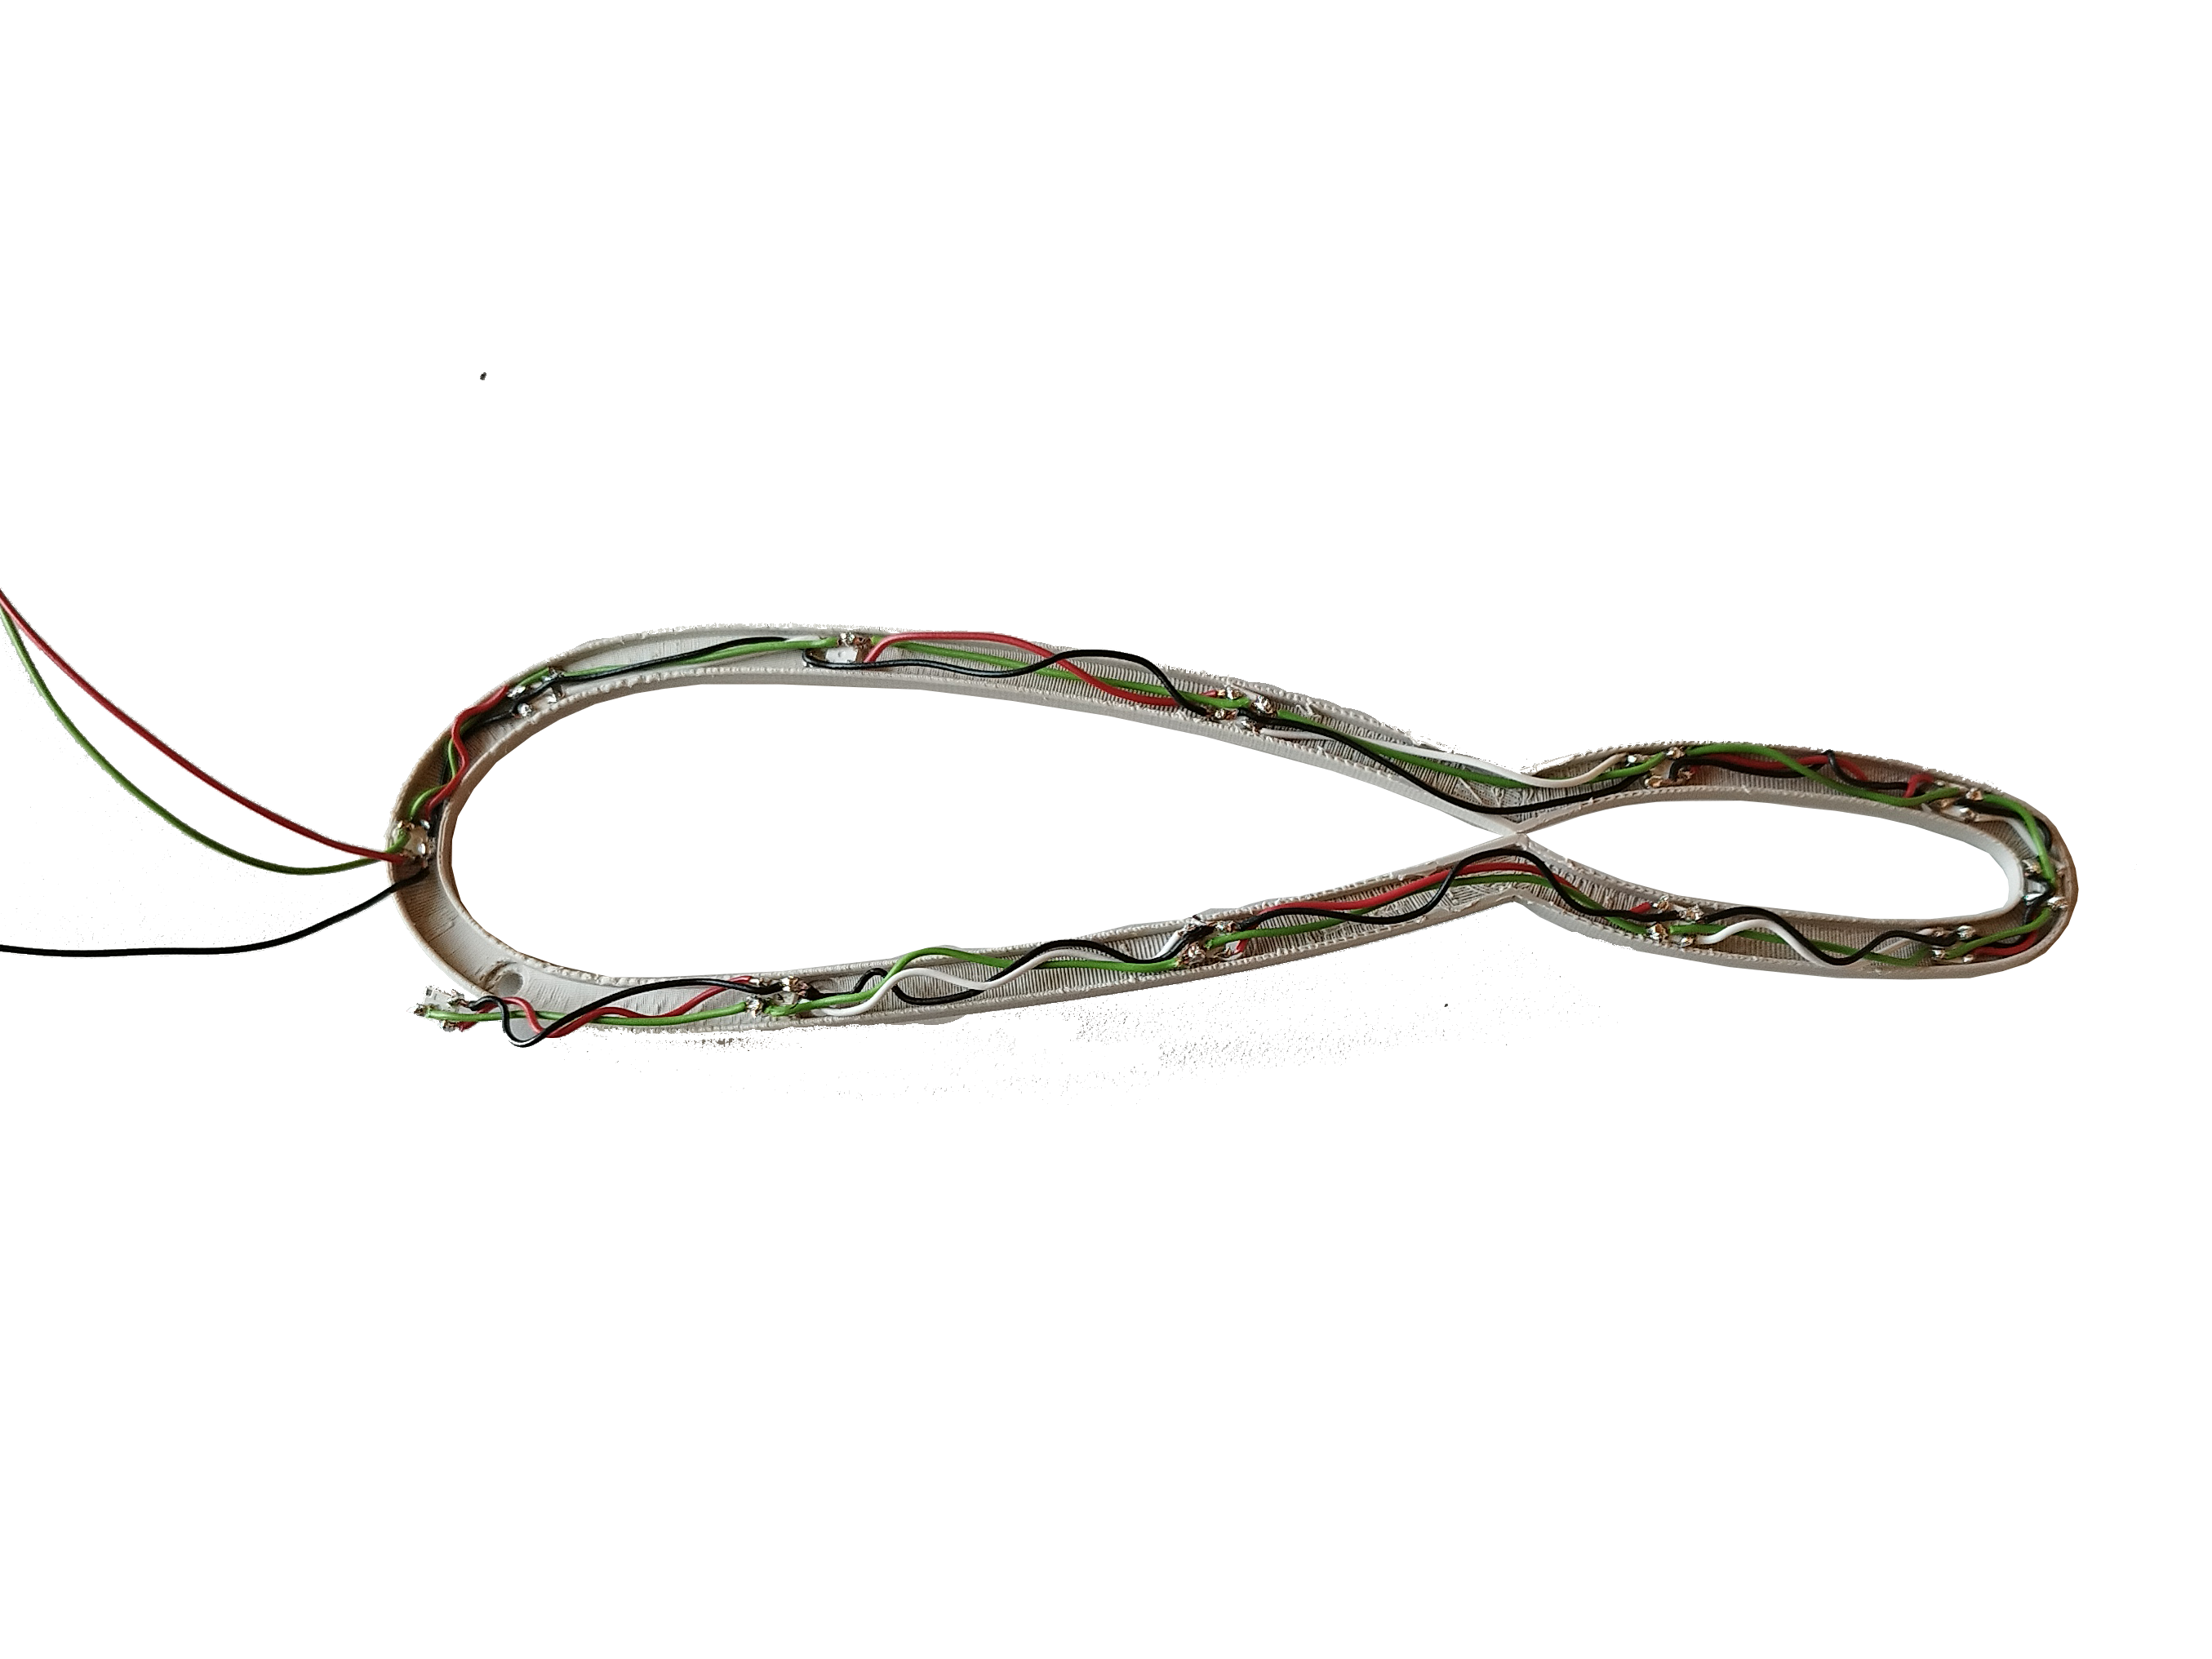
\includegraphics[width=\linewidth]{Images/cable.png}        
        \captionof{figure}{Cabel layout in a real world setup}
        \label{cabel}

    \end{figure}
    \end{minipage}
    

\newpage


\section{The first user feedback }
\label{feedback}

  A first prototype was completed in time for the "Bright environments: Daylight in Sustainable Building Design Conference". User feedback was gathered through this opportunity and the model was modified accordingly.
 \begin{multicols}{2}
  This opportunity resulted in me assembling many analemmas for the first time. After testing all analemmas individually, all of them worked. However assembling all seven and plugging them into the Arduino introduced new problems. The analemma did not behave as expected and showed very random behaviour. After some investigation, the problem was identified to be the Arduino itself. The high number of analemmas forced the Arduino to process more data and control more LED lights. Even though the build was small enough at compilation time, it would produce as much control data for the LEDs at runtime, that the Arduino simply ran out of SRAM and started to behave unpredictably. Thus, a state with reduced functionality and no turning knob was created for the presentation at the conference. This problem was later addressed by choosing another more powerful version of the Arduino
  \columnbreak
  (Arduino Due instead of Arduino Uno Rev3). As a result of that problem, the knob control was not fully functional at the time of presentation and could thus not be tested with the audience.\\
  \\
  Generally, the feedback of the people was very positive. This day showed, that visitors are generally attracted and interested by things which glow, and that the representation of the sun path as analemmas was not questioned by the daylight experts and thus must have been understandable. Very importantly, this day showed the need to provide a color legend and reminded me, that certain words specific to our field might not be in everybody's vocabulary and either need to be explained or omitted completely. As a general feedback though, the concept was understood well and no critical issues were pointed out.\\  
\end{multicols}
\begin{minipage}{0.48\linewidth}
        \centering
        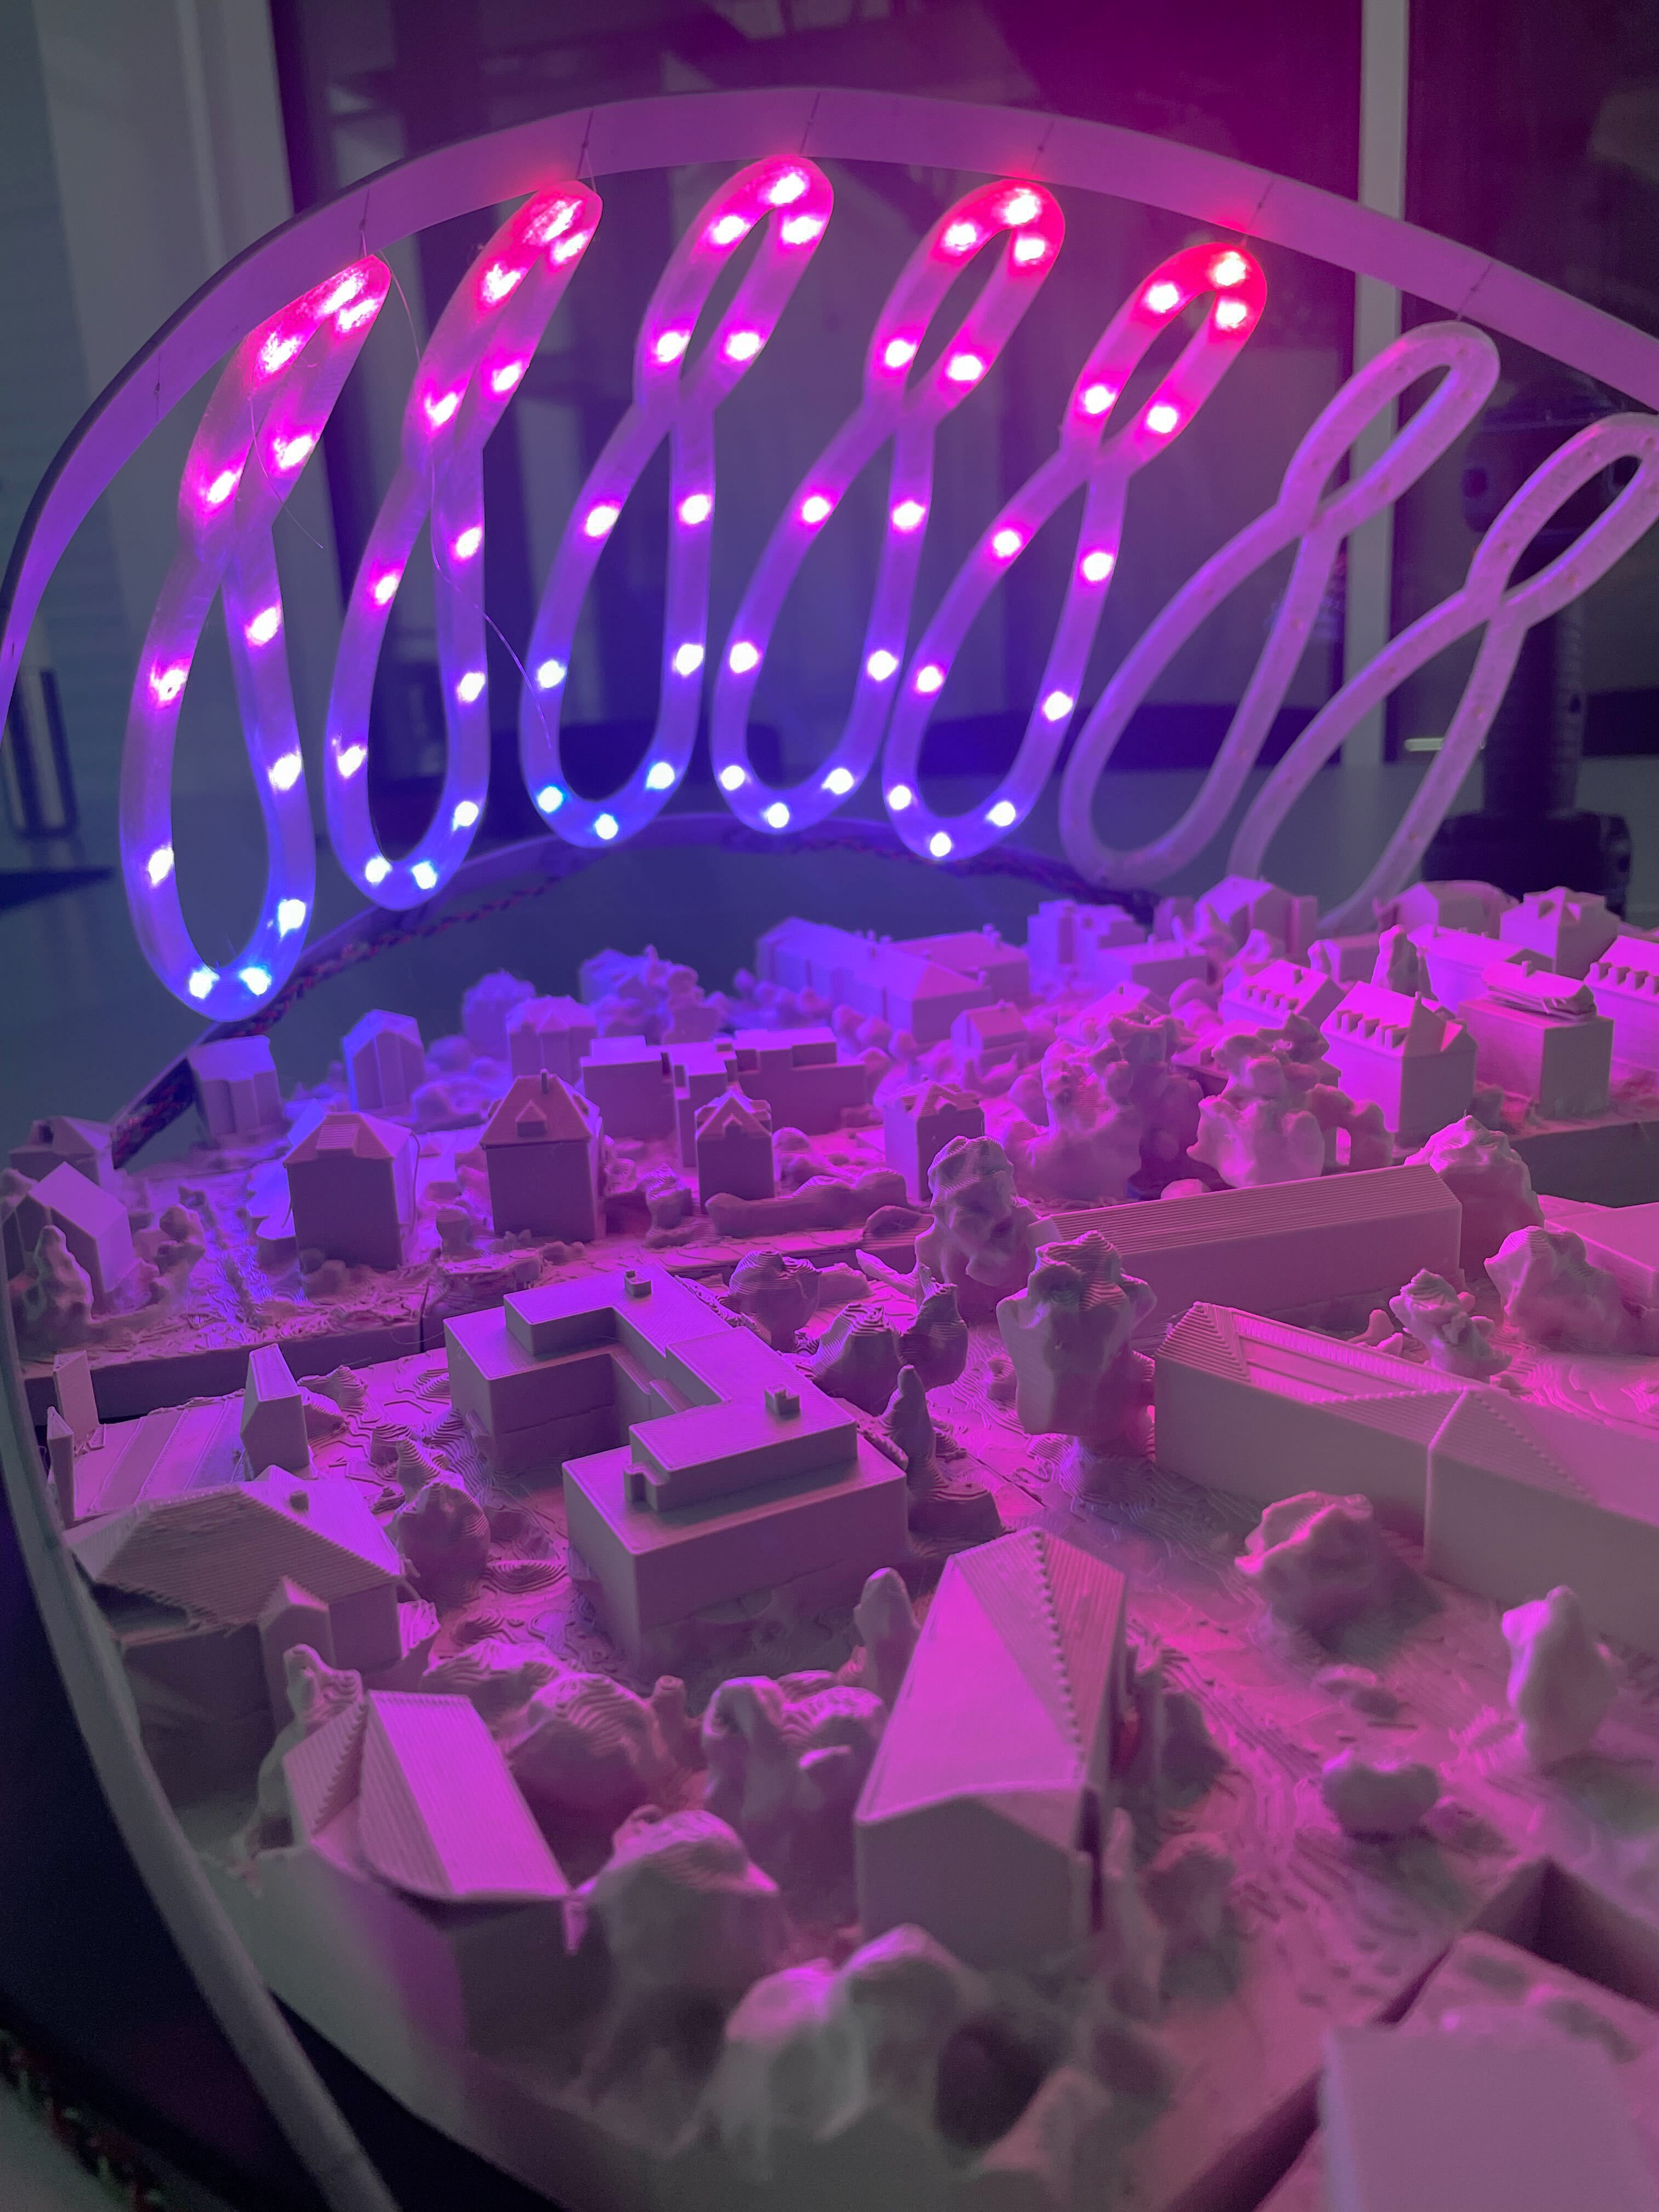
\includegraphics[width=.59\linewidth]{Images/img_6557.jpg}
  
        \caption{Temperature visualised for Zurich}
        
    \end{minipage}
    \hfill
    \begin{minipage}{0.48\linewidth}
         \centering
        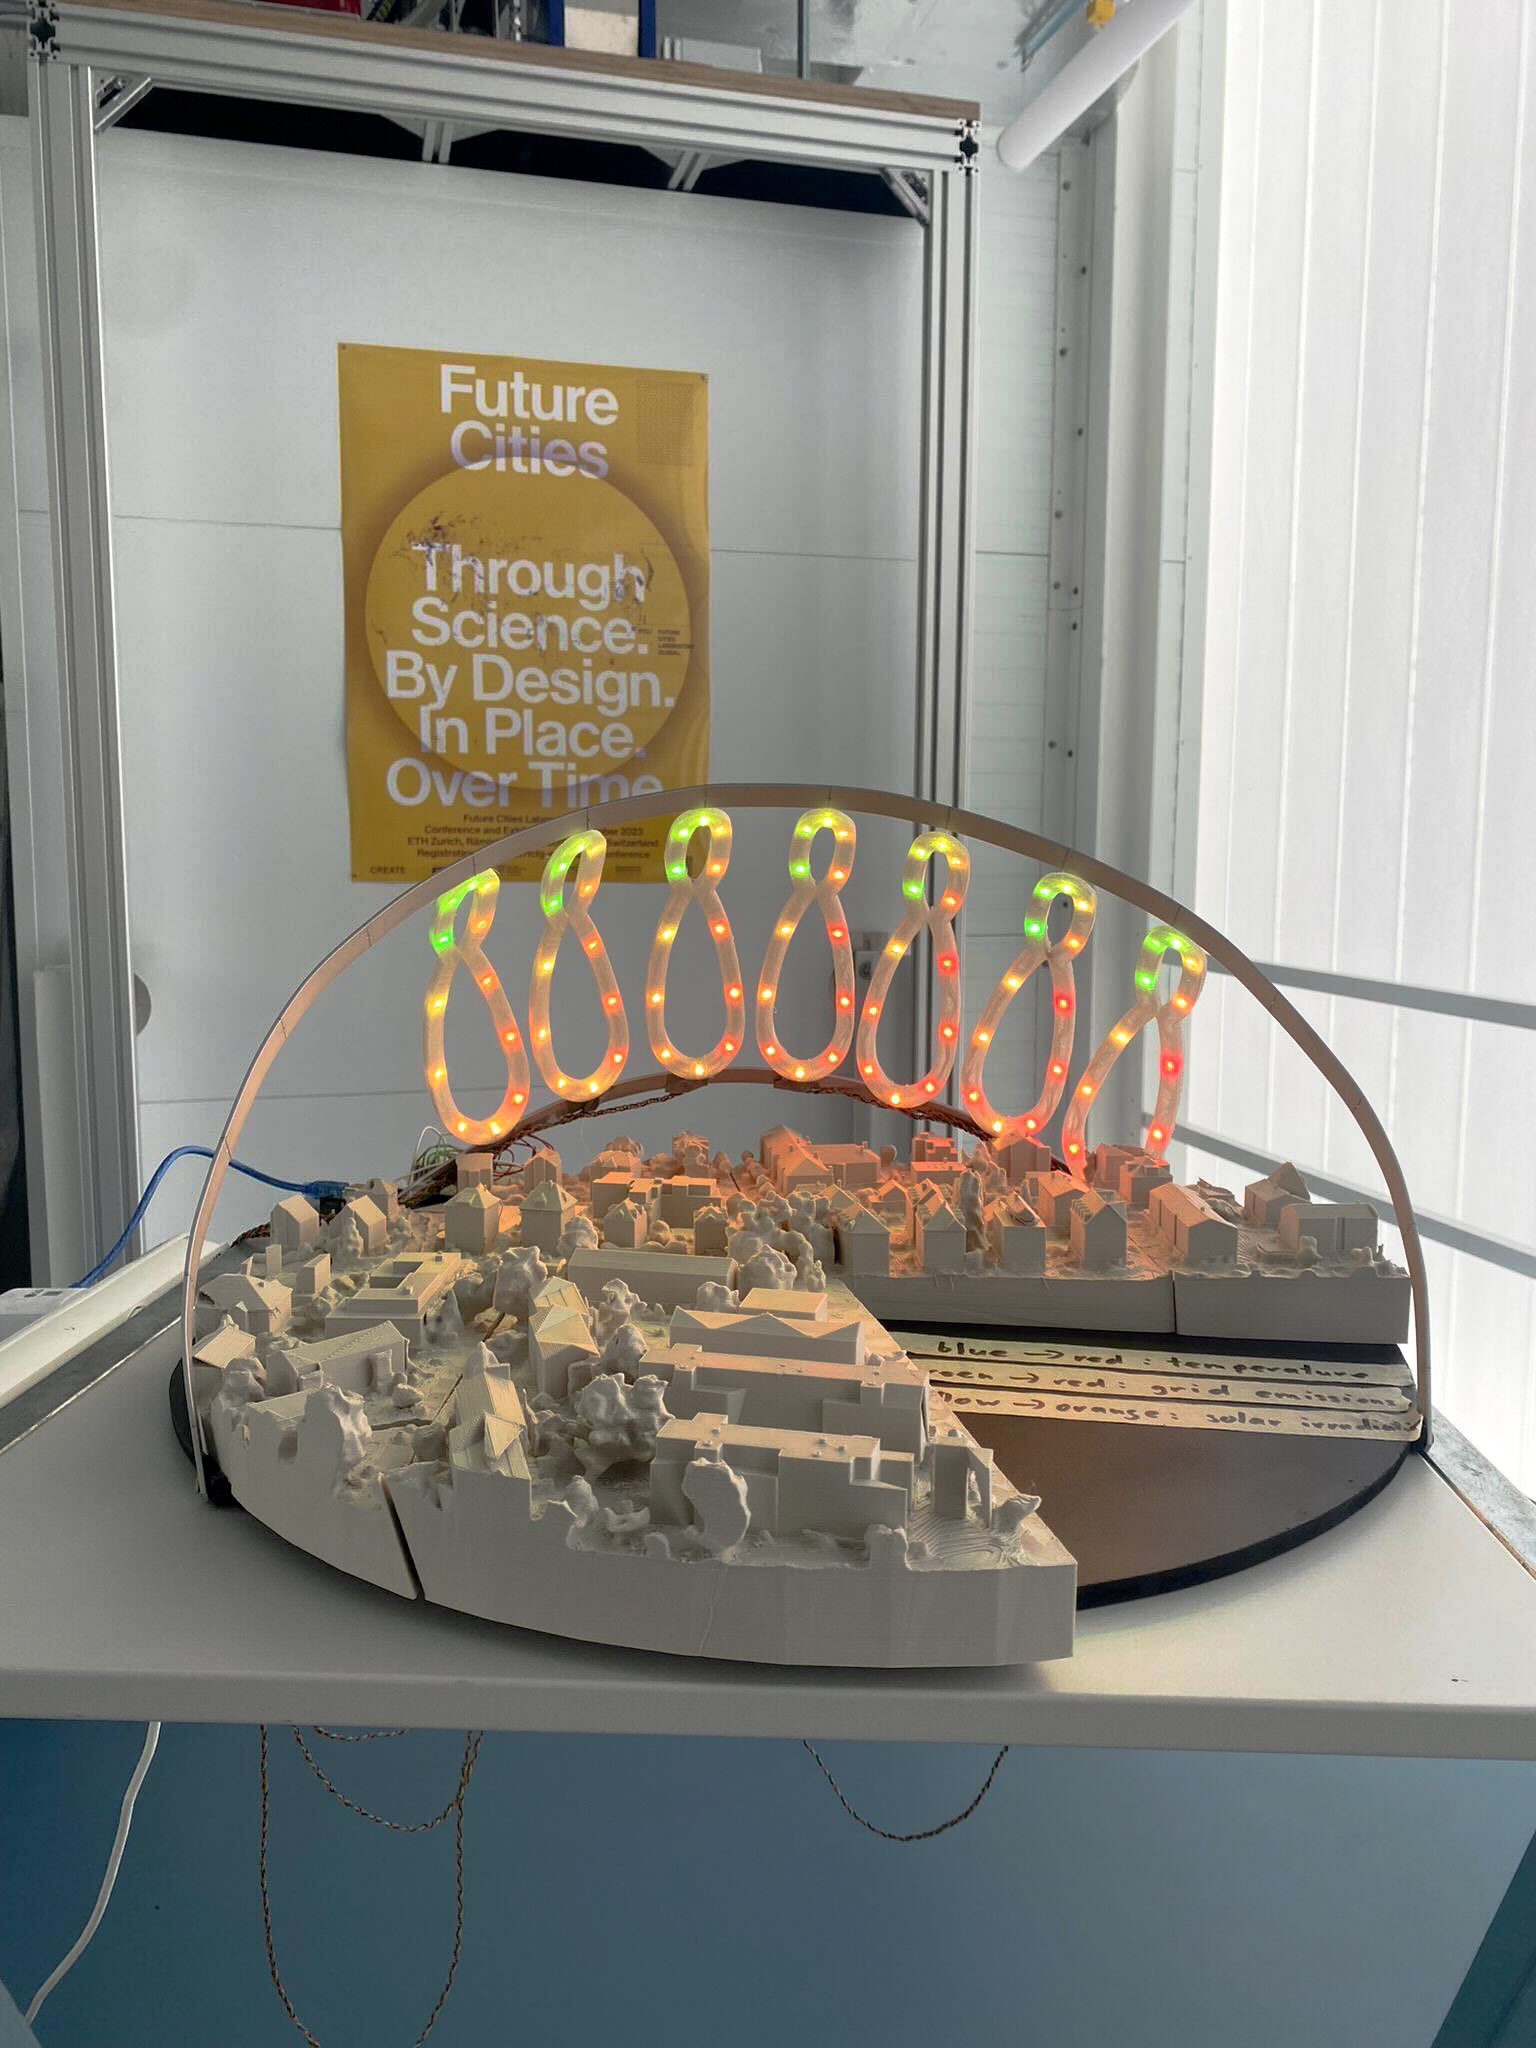
\includegraphics[width=.59\linewidth]{Images/e32895bd-aff2-495c-9af3-a0f7fa5a6cf7.jpg}
     
        \caption{Grid emission visualised for Zurich}
        
    \end{minipage}
    \begin{minipage}{0.48\linewidth}
        \centering
        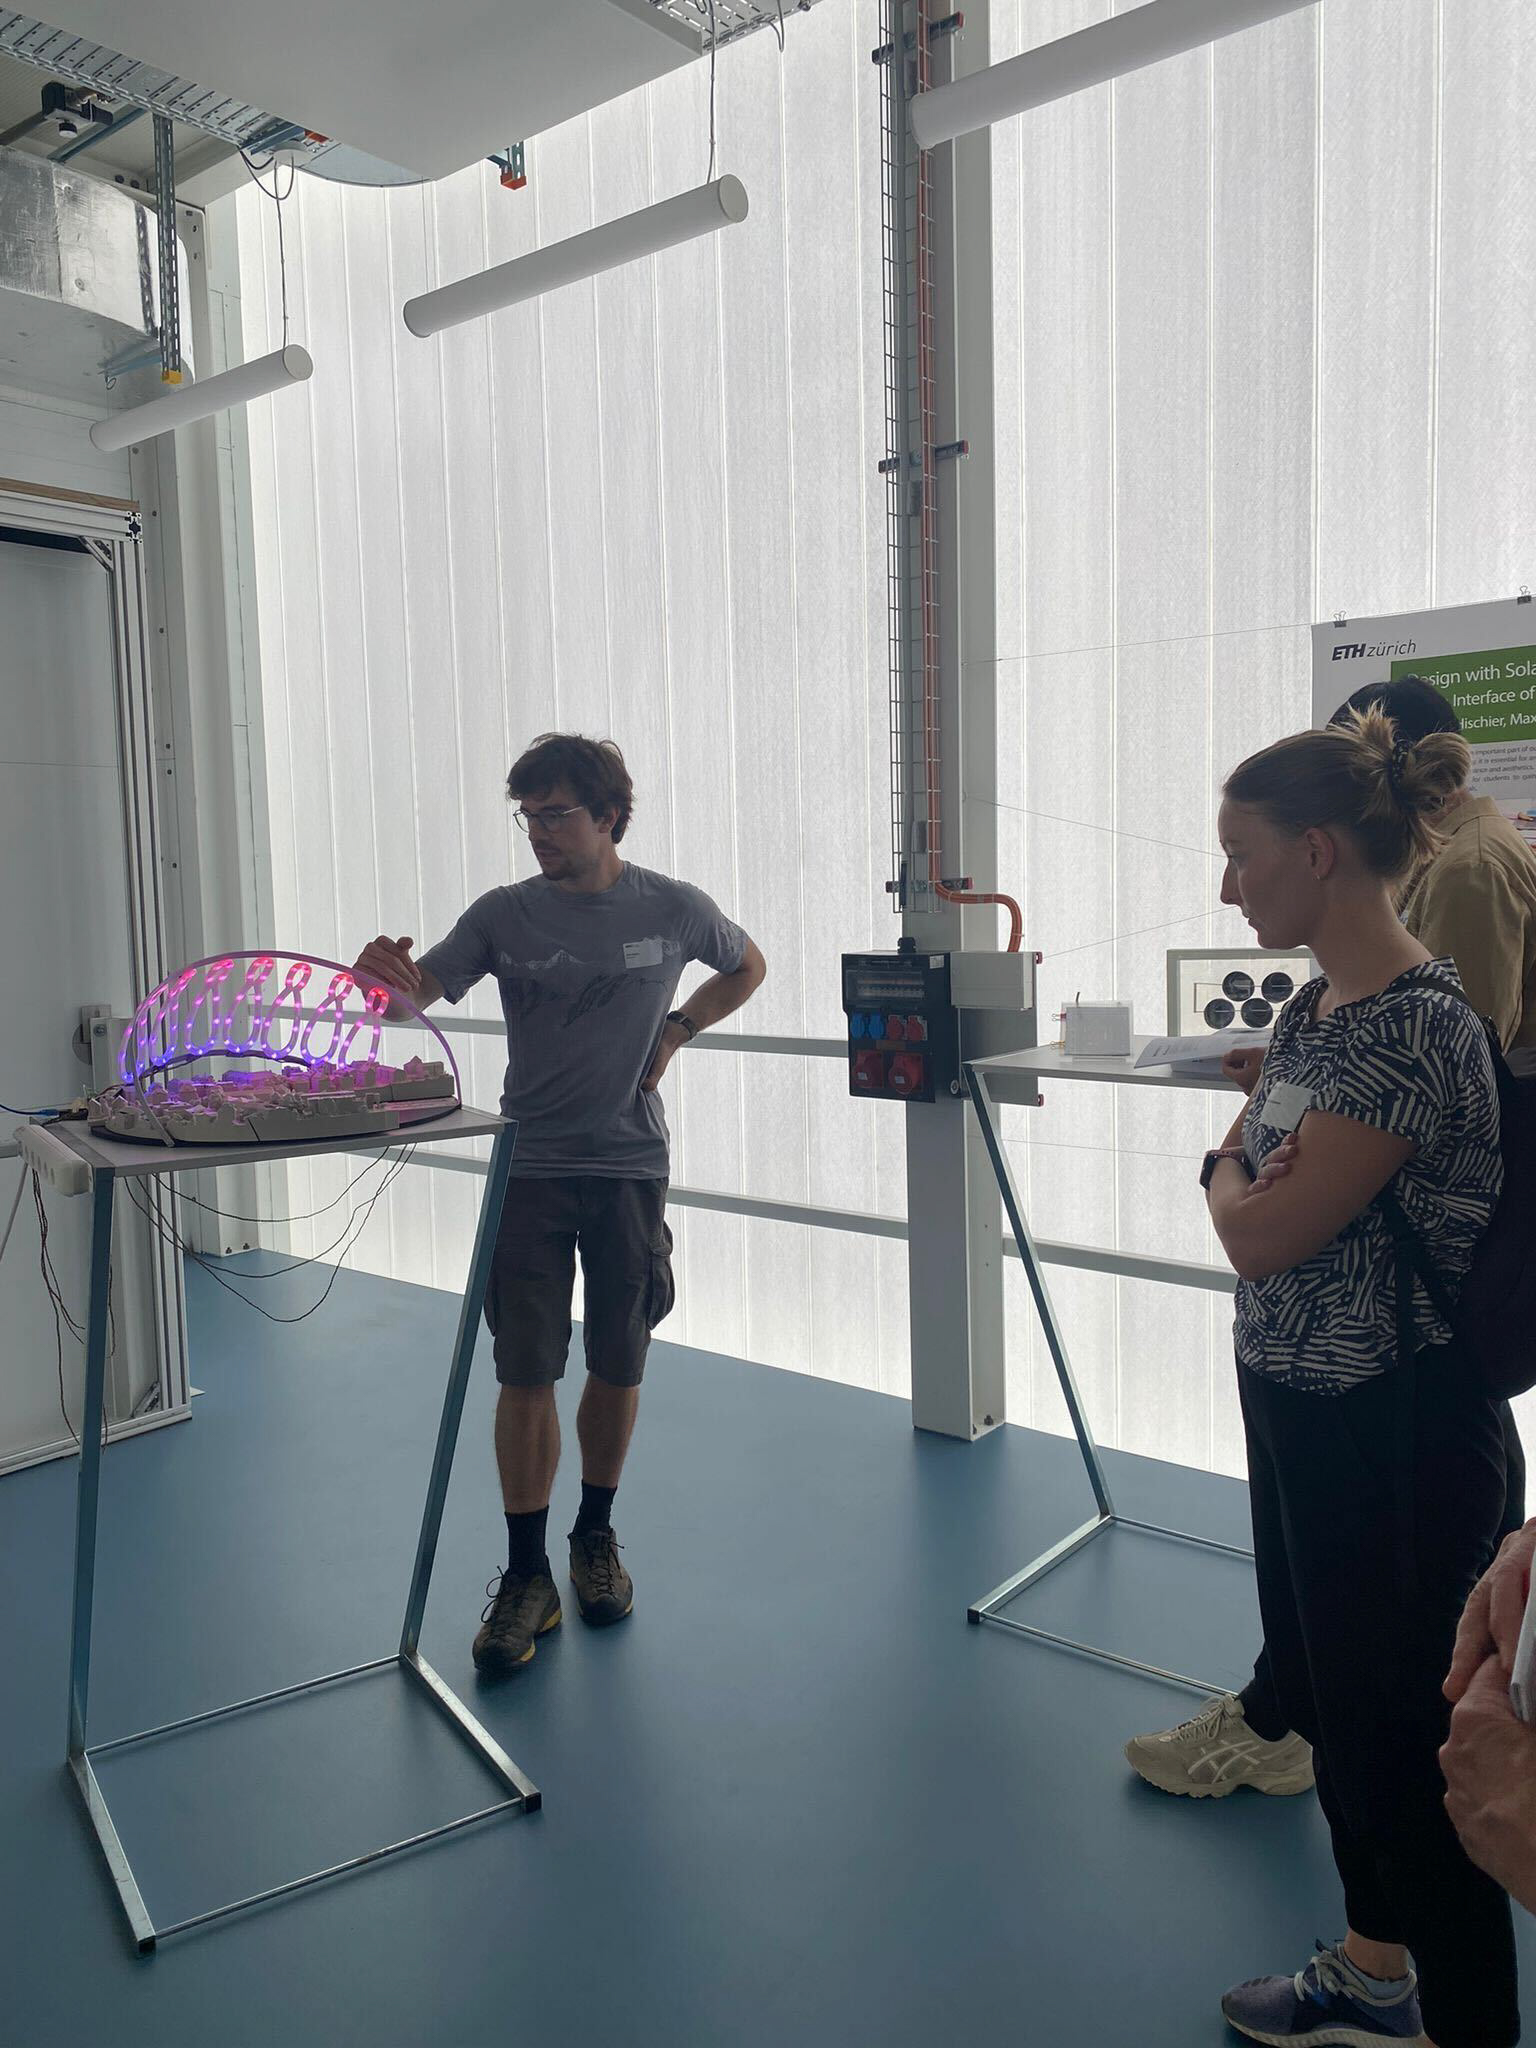
\includegraphics[width=.59\linewidth]{Images/b9d45c07-98a5-4d7e-ab01-3ffce05beceb.jpg}
        \caption{The presentation to the audience}
        
    \end{minipage}
     \hfill
    \begin{minipage}{0.48\linewidth}
         \centering
        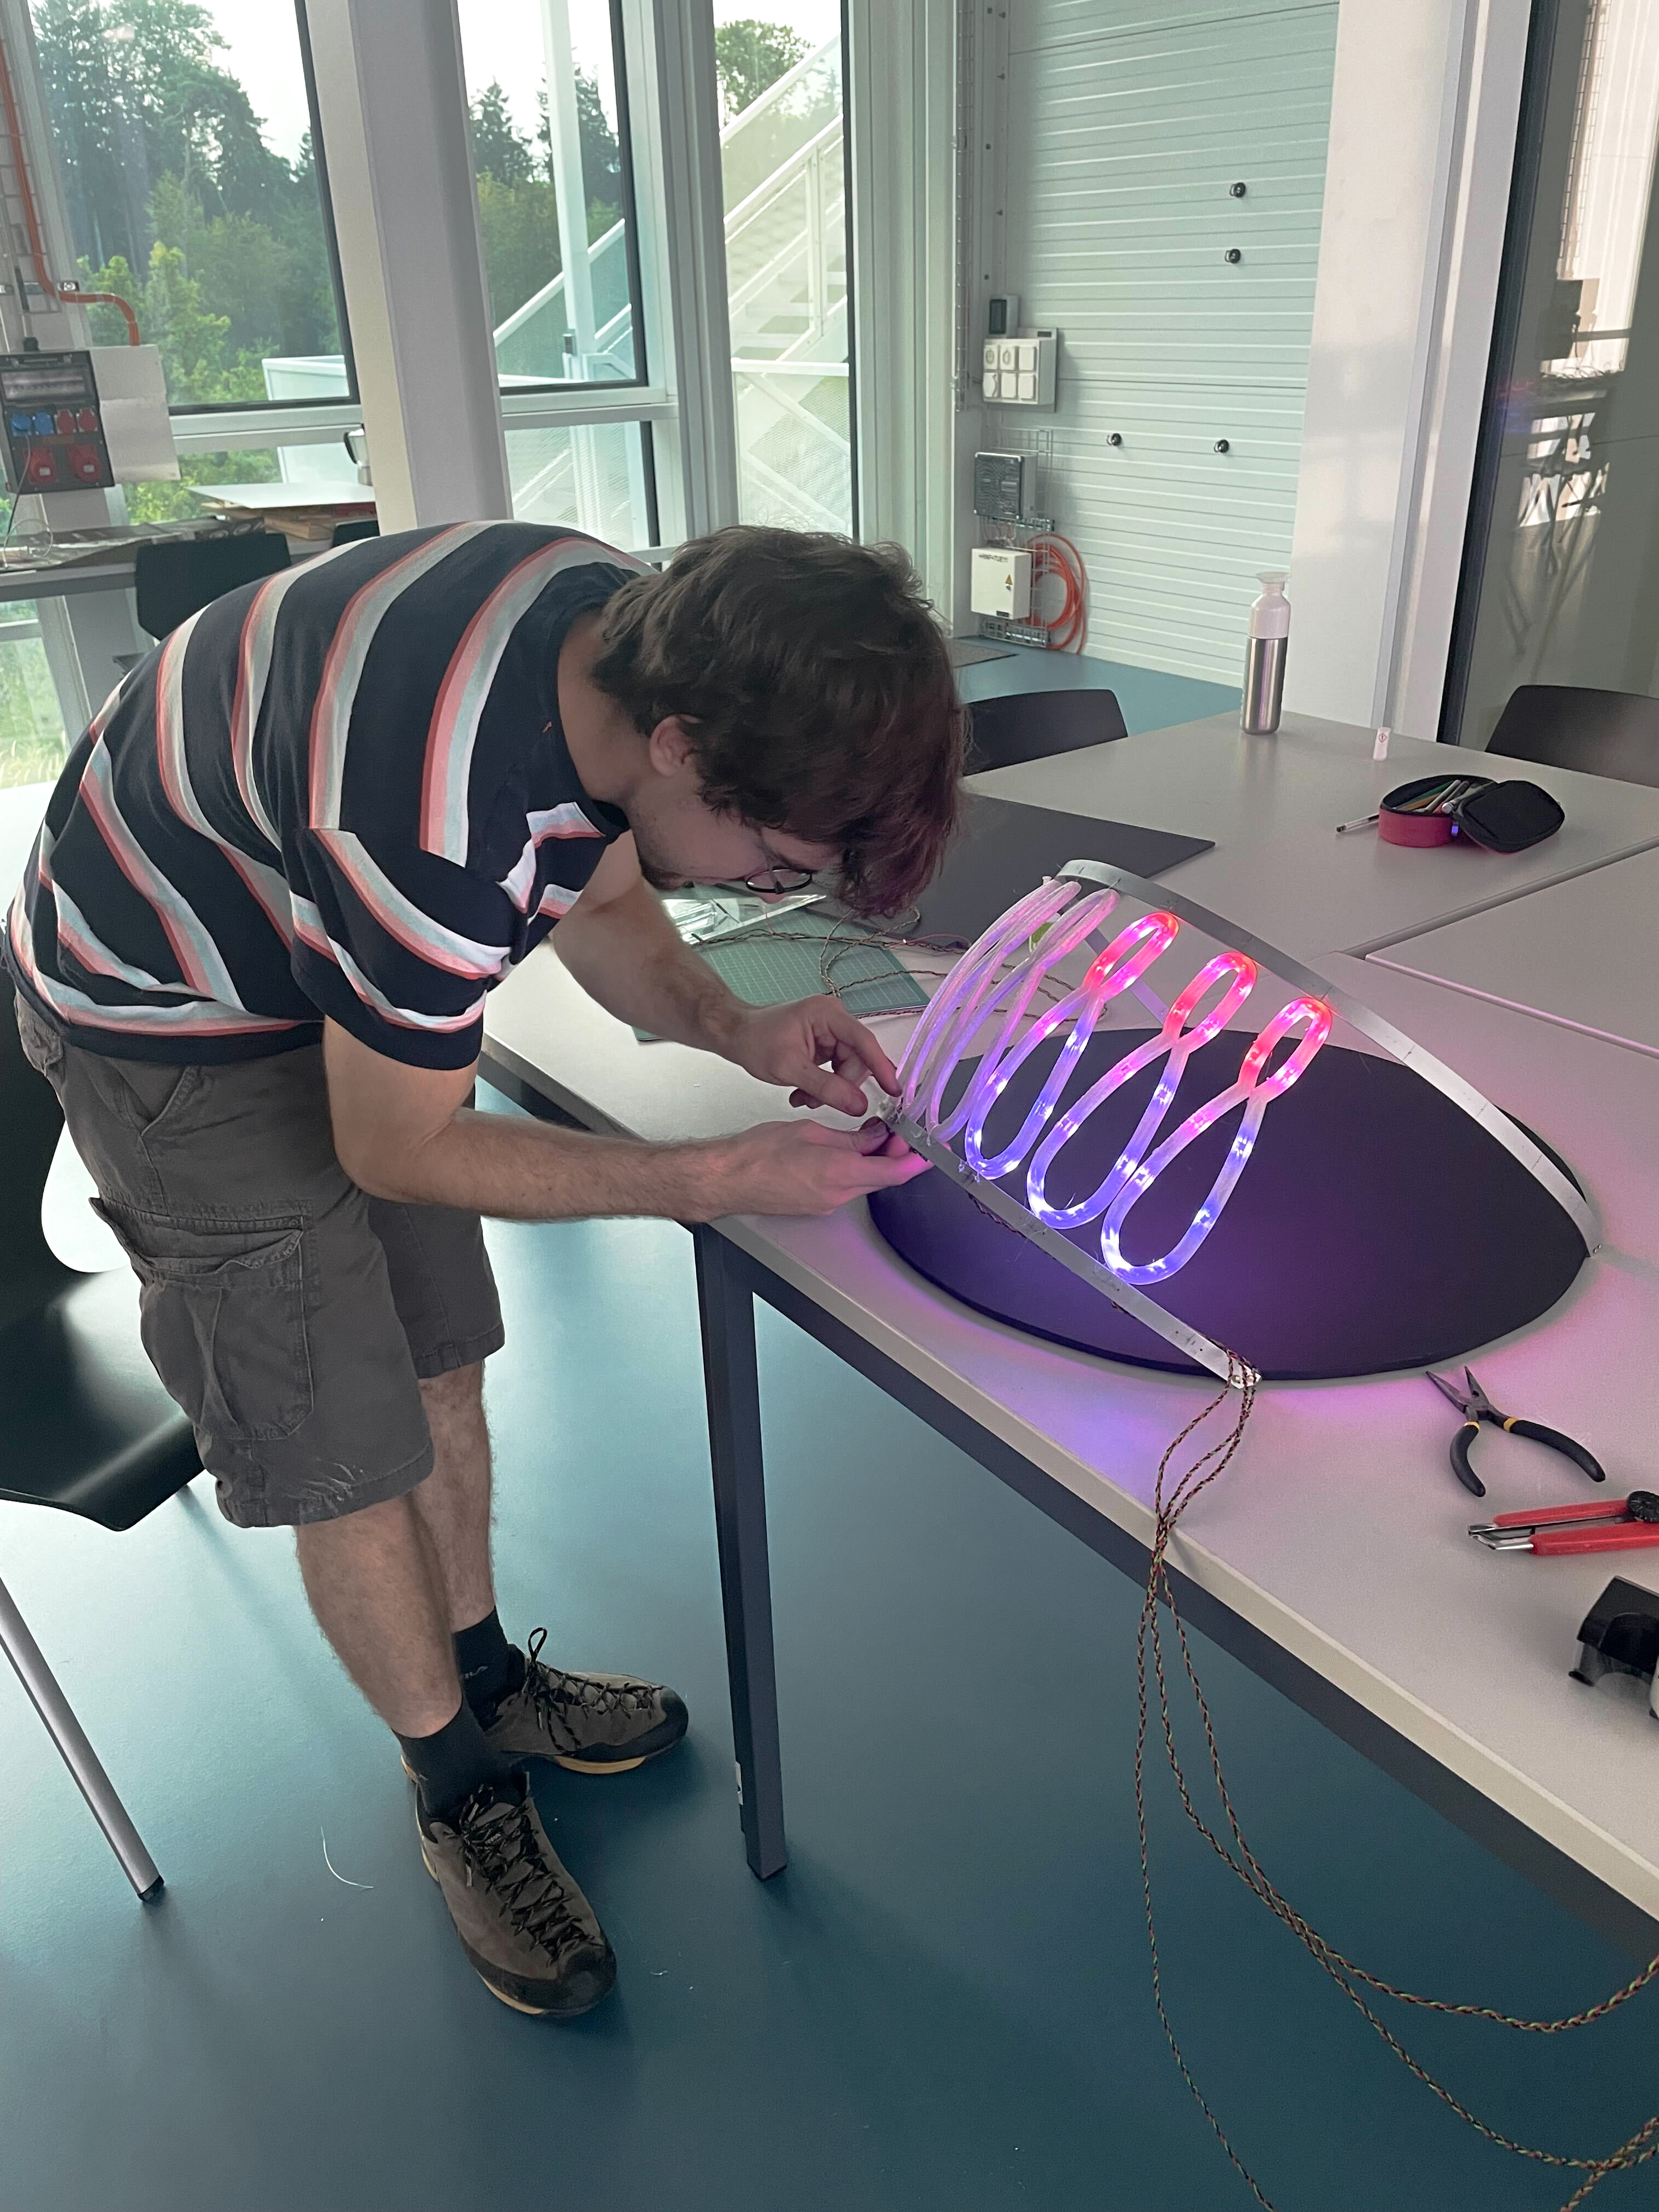
\includegraphics[width=.59\linewidth]{Images/img_6556.jpg}
        \caption{Assembly of the first bigger prototype}
        
    \end{minipage}
    

\newpage
\section{Details of the final design}
After the general concept was fixed (cf. \textit{Section} \ref{light}) and the first presentation with user feedback was over (cf. \textit{Section} \ref{feedback}), the production of the final model started. The 3D city model has been printed, a MDF base to host the model and to attach the sun path has been developped, the shape of the analemma has been reworked and the user interface/experience has been developed and improved to its final state, using the new Arduino Due, turning knobs and a LCD Display. As a last step a box has been developped to hide away the Arduino with the cables and to house the user interface and LCD screen (cf. \textit{Section} \ref{box}). \\
\\
This final version of the setup (cf. \textit{Figure} \ref{final}, \ref{fin1}, and \ref{fin2}) is described to all details in the following sections.
\\[1cm]
\begin{figure}[H]
    \centering
    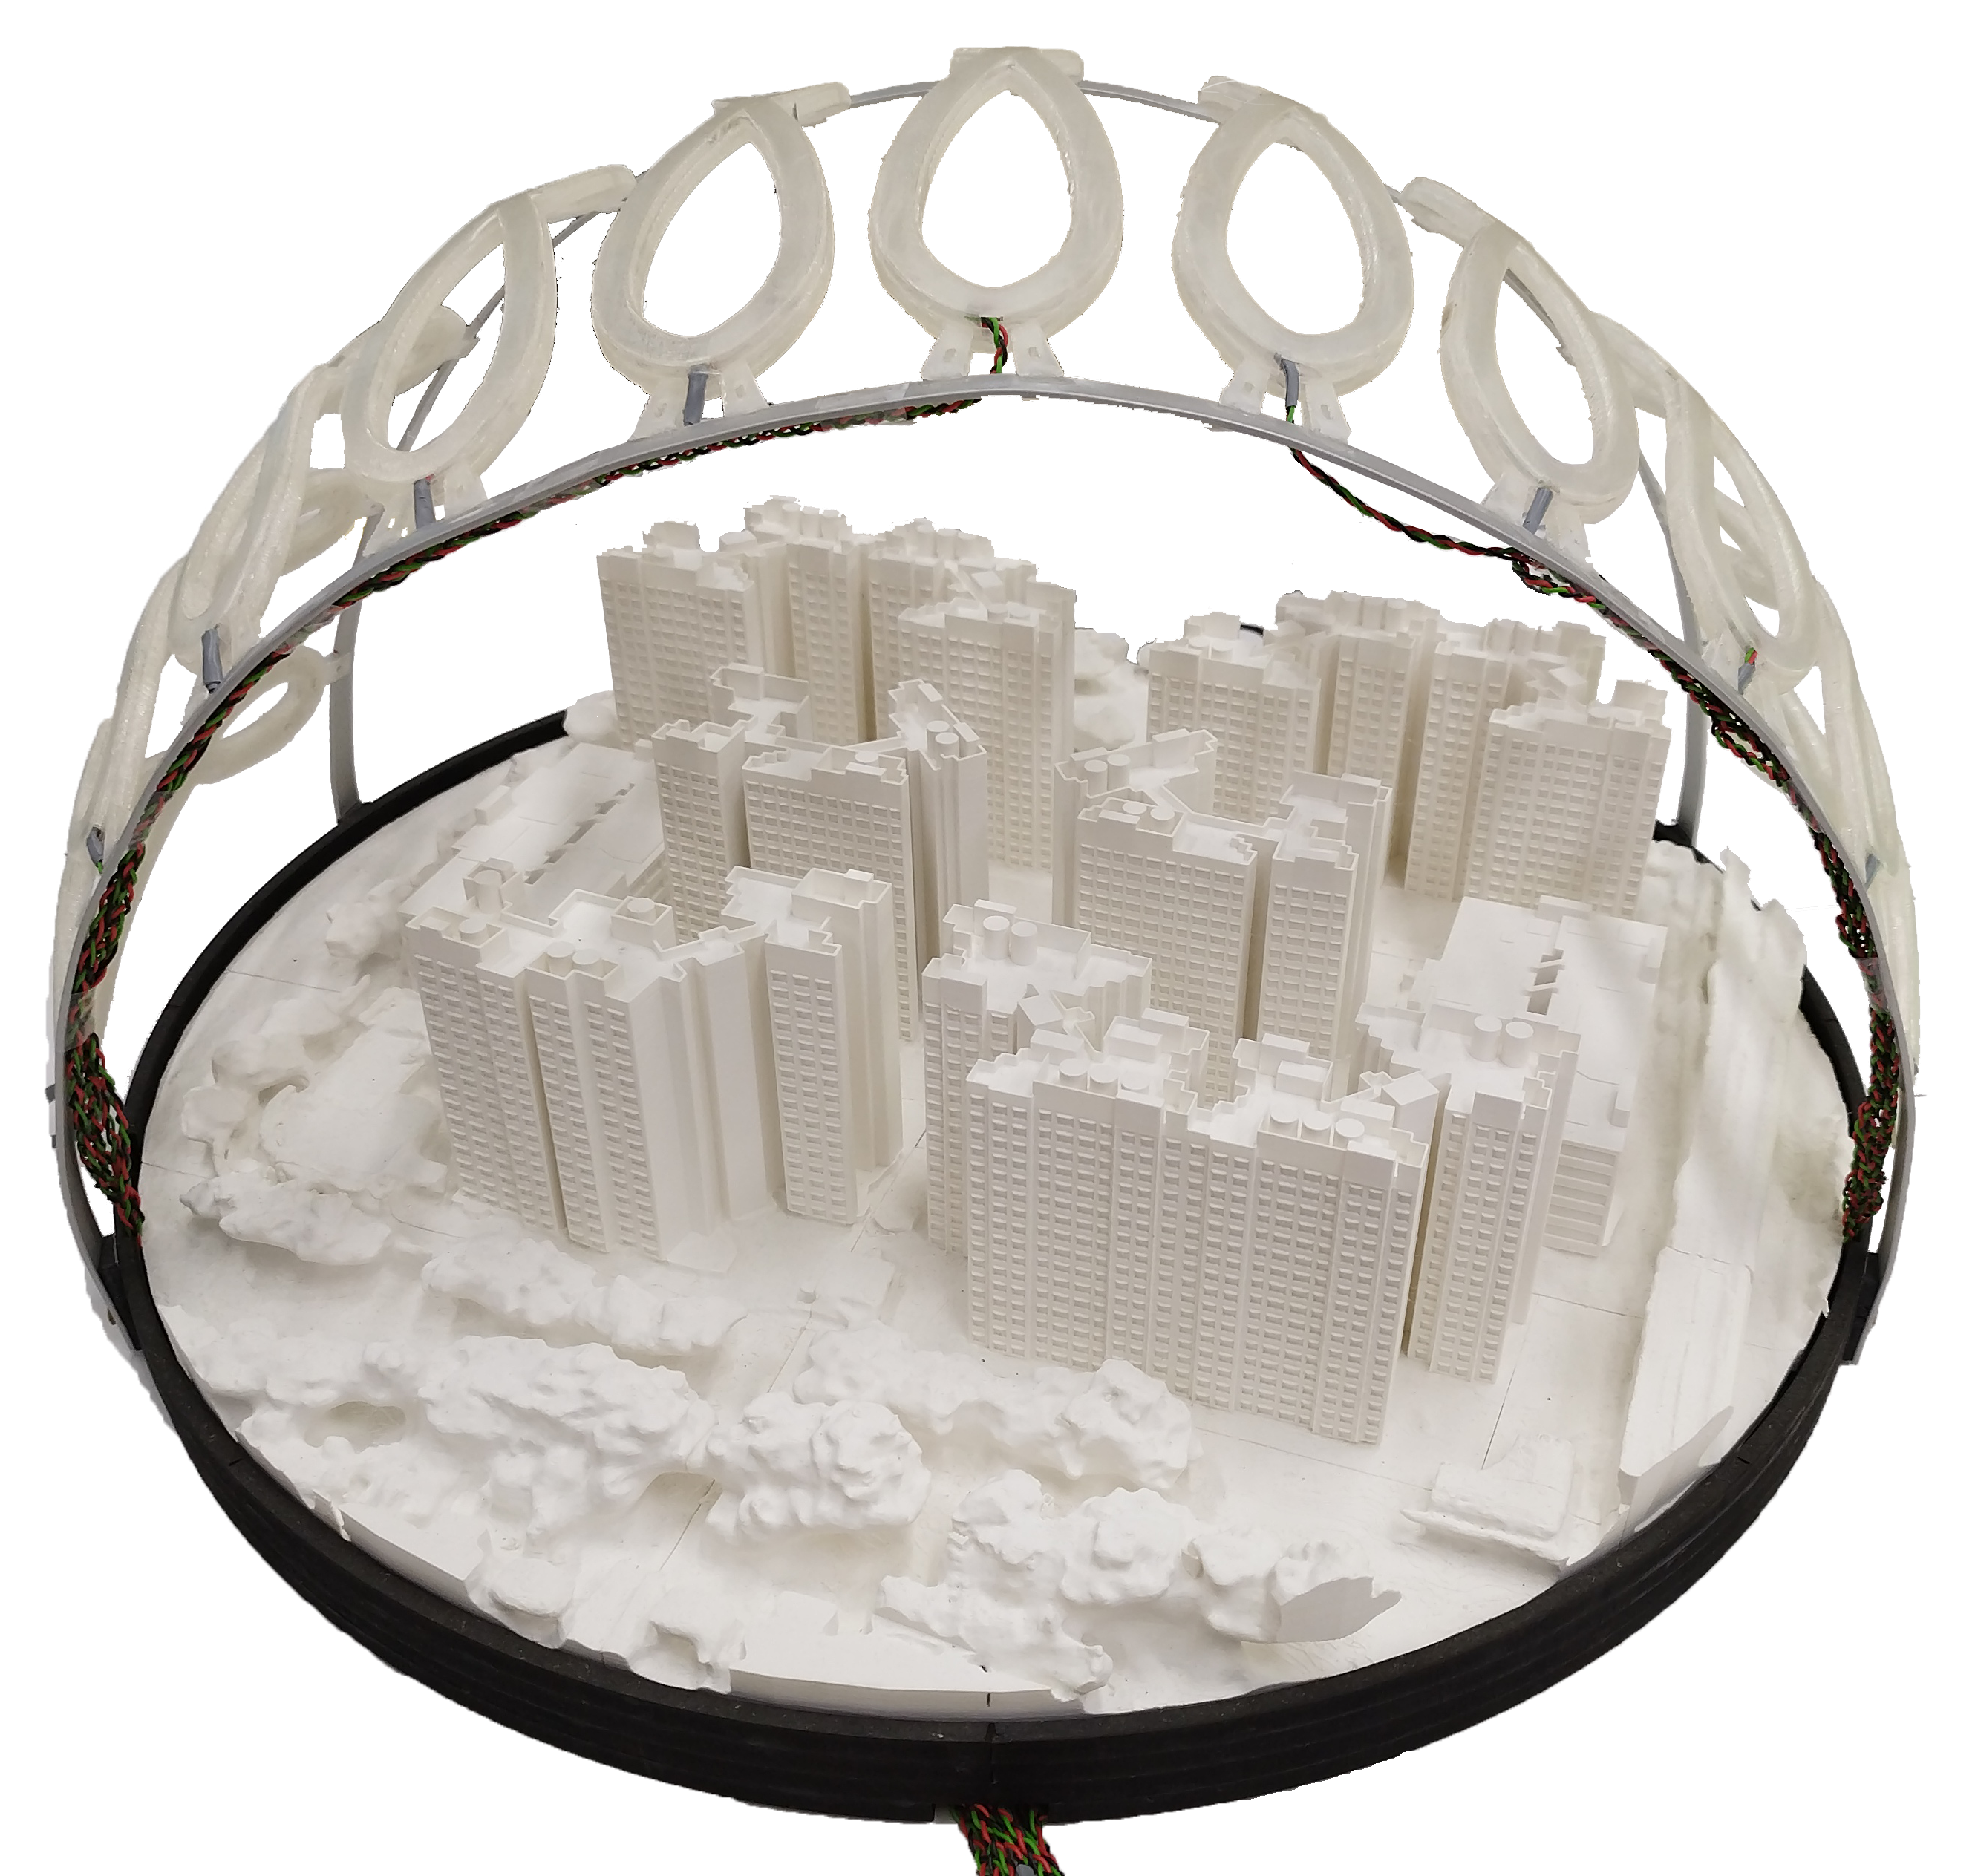
\includegraphics[width=\linewidth]{Images/final.png}
    \caption{Final Setup for Singapore}
    \label{final}
\end{figure}
\newpage
\begin{multicols}{2}
    [
    \subsection{The 3D printed city model}
    ]
    To position the visualized sunpaths in a concrete geographical location, a model of the city at the studied places was printed out. These two models were based on a photogrammetry scan of google earth terrain done by Gregory Bianchi and then completed with hand modeled buildings by Chen Chiu (Rachel) and Christoph Waibel. For the prints a white PLA was used. To benefit from the high amount of detail a FDM print can offer, the layer height was set to 0.2mm with a nozzle diameter of 0.4mm. (For more details see the g-codes). The model was split into pieces as the dimensions of the printer are limited to 25cmx20cmx20cm and later on glued together again. The scale of the model was chosen, such that it is approximately 1:500 for both locations.
\end{multicols}

\begin{minipage}{0.48\linewidth}
        \centering
        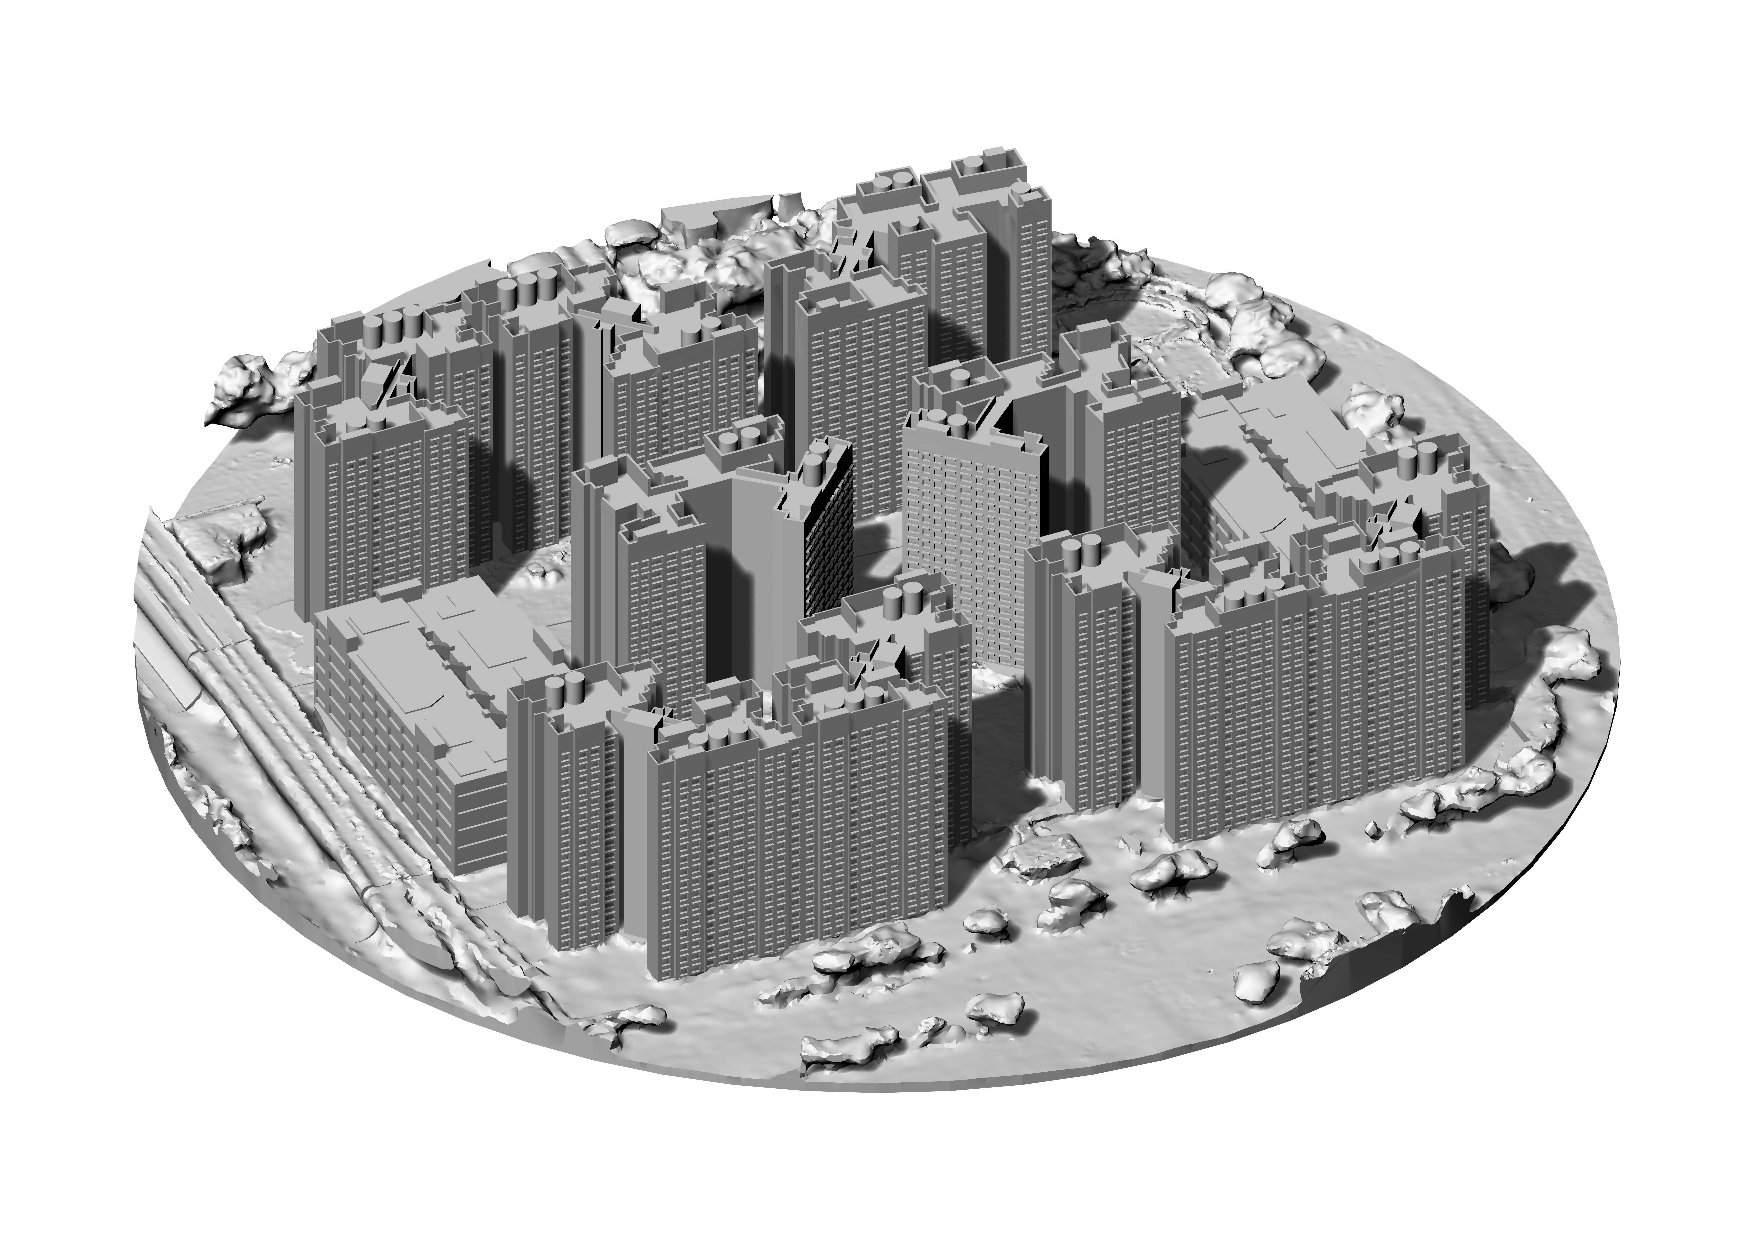
\includegraphics[width=\linewidth]{Images/modelsg.pdf}
       \\{Singapore}
         \label{model sg}
    \end{minipage}
    \hfill
    \begin{minipage}{0.48\linewidth}
         \centering
        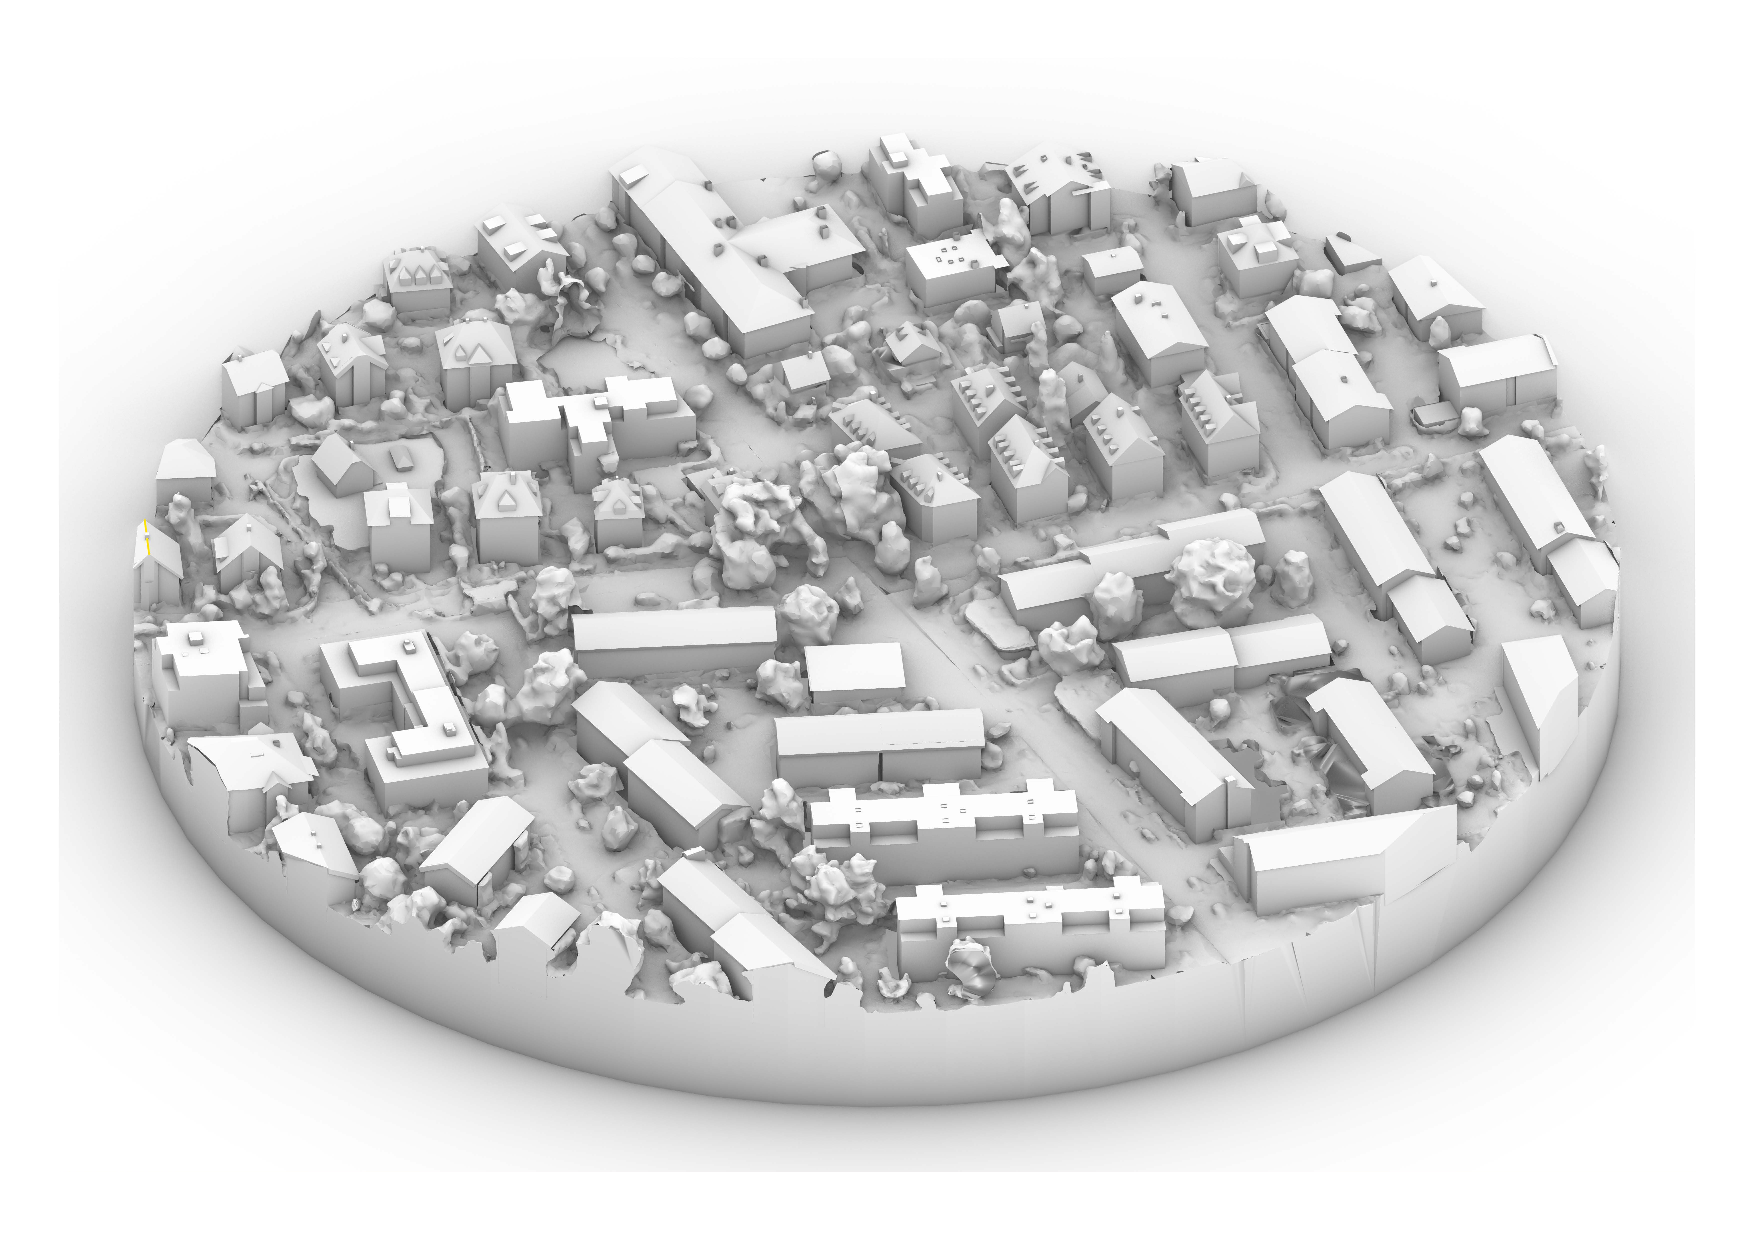
\includegraphics[width=.85\linewidth]{Images/modelzh.pdf}
       \\{Zurich}
        \label{model zh}
    \end{minipage}
    \captionof{figure}{Data for the 3D printed model}
    \begin{minipage}{0.48\linewidth}
        \centering
        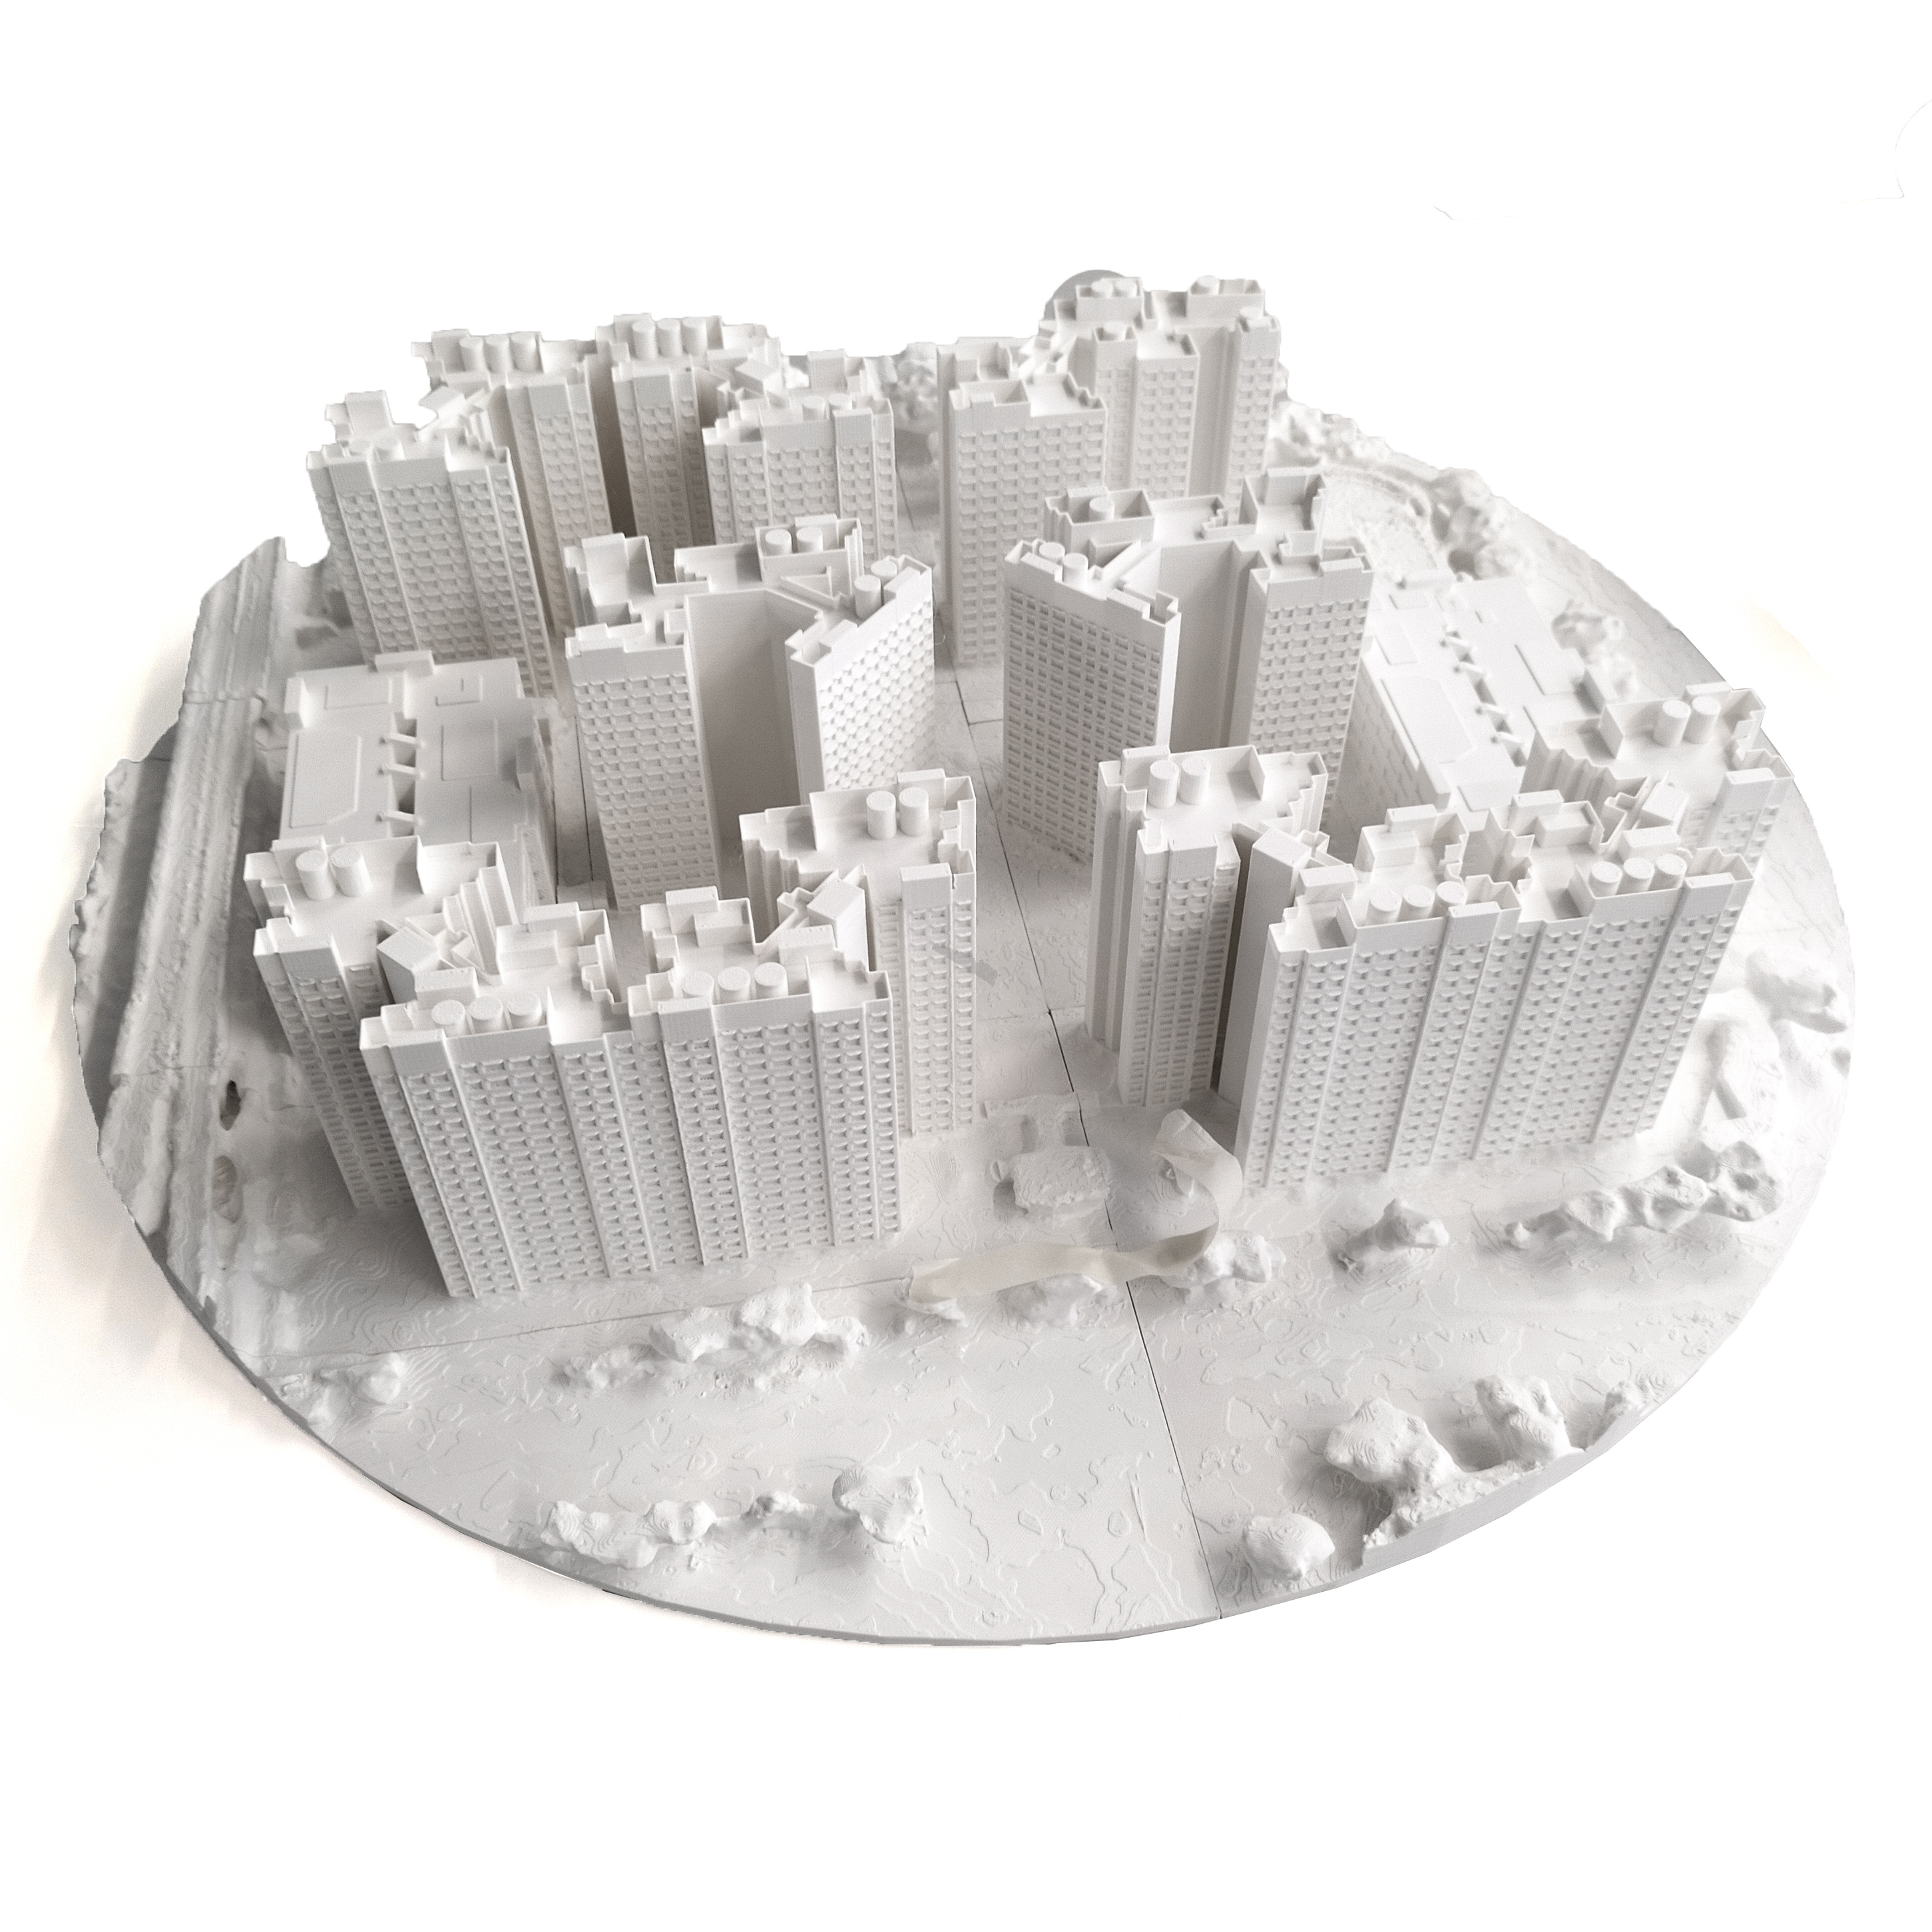
\includegraphics[width=.7\linewidth]{Images/modSG_1.jpg}
       \\{Singapore}
         \label{modelp sg}
    \end{minipage}
    \hfill
    \begin{minipage}{0.48\linewidth}
         \centering
        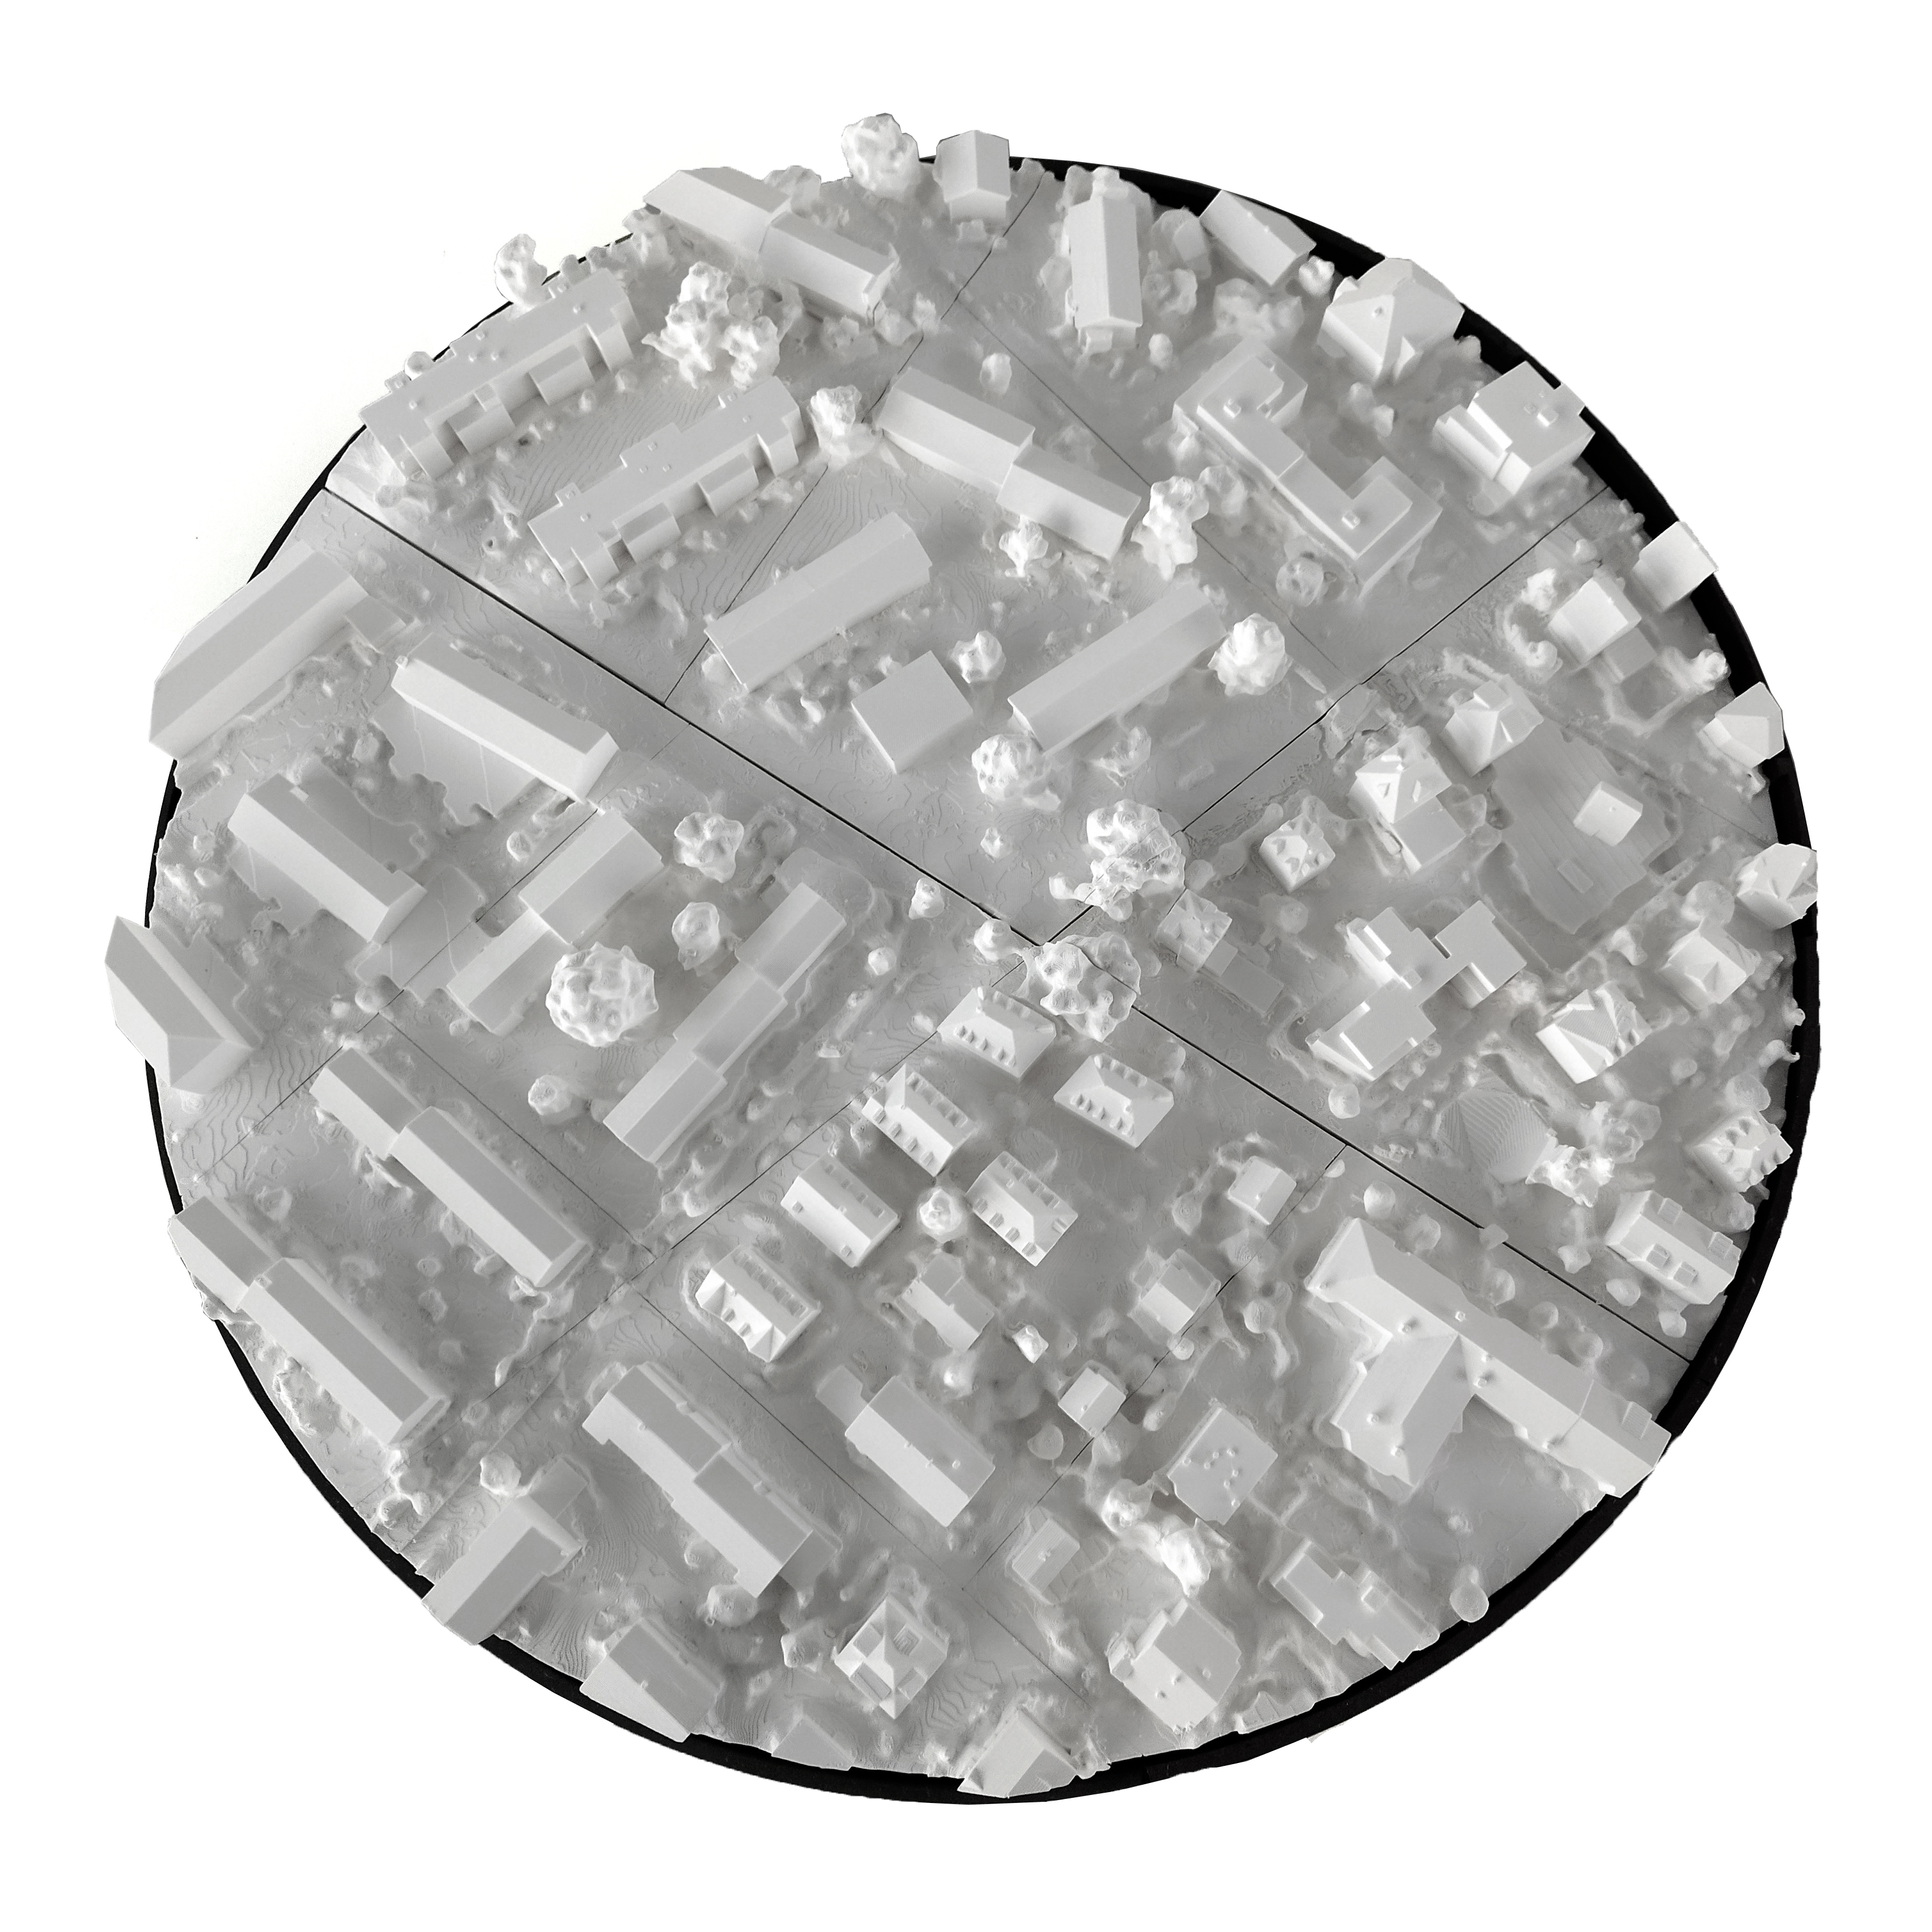
\includegraphics[width=.85\linewidth]{Images/modZH_1.jpg}
       \\{Zurich}
        \label{modelp zh}
    \end{minipage}
    \captionof{figure}{Pictures of the finished printed model}
\newpage
\begin{multicols}{2}
[
\subsection{The base}
]
    In addition to the model, a base was developed. The bases main purpose is to frame the white model with its black color and to provide hidden space and slits for cable management as well as to provide a solid volume to anker the metal support profiles of the sun path (cf. \textit{Figure} \ref{baseee}).\\
    \\
    A first experimentation with cutting MDF into a round shape by hand failed. To achieve the precision and the rather small thicknesses around the cable management slits (cf. \textit{Figure} \ref{cuuuut2} and \ref{cuuuut}) and the border a laser cutter was used (executed by Schnittstelle Altstetten). Scaling the slits and the border to larger dimensions was not possible, as the size of the model was limited by the layout of the other content on the table. The base was glued together using wood glue. Later on additional holes next to the cable management slits were drilled to allow easier insertion of the cables into the slit. The models were fixed inside the base with velcro tape, such that they can still be removed, if changes need to be made to the cable or if a cable needs to be removed.
\end{multicols}

  \begin{minipage}{0.48\linewidth}
        \centering
        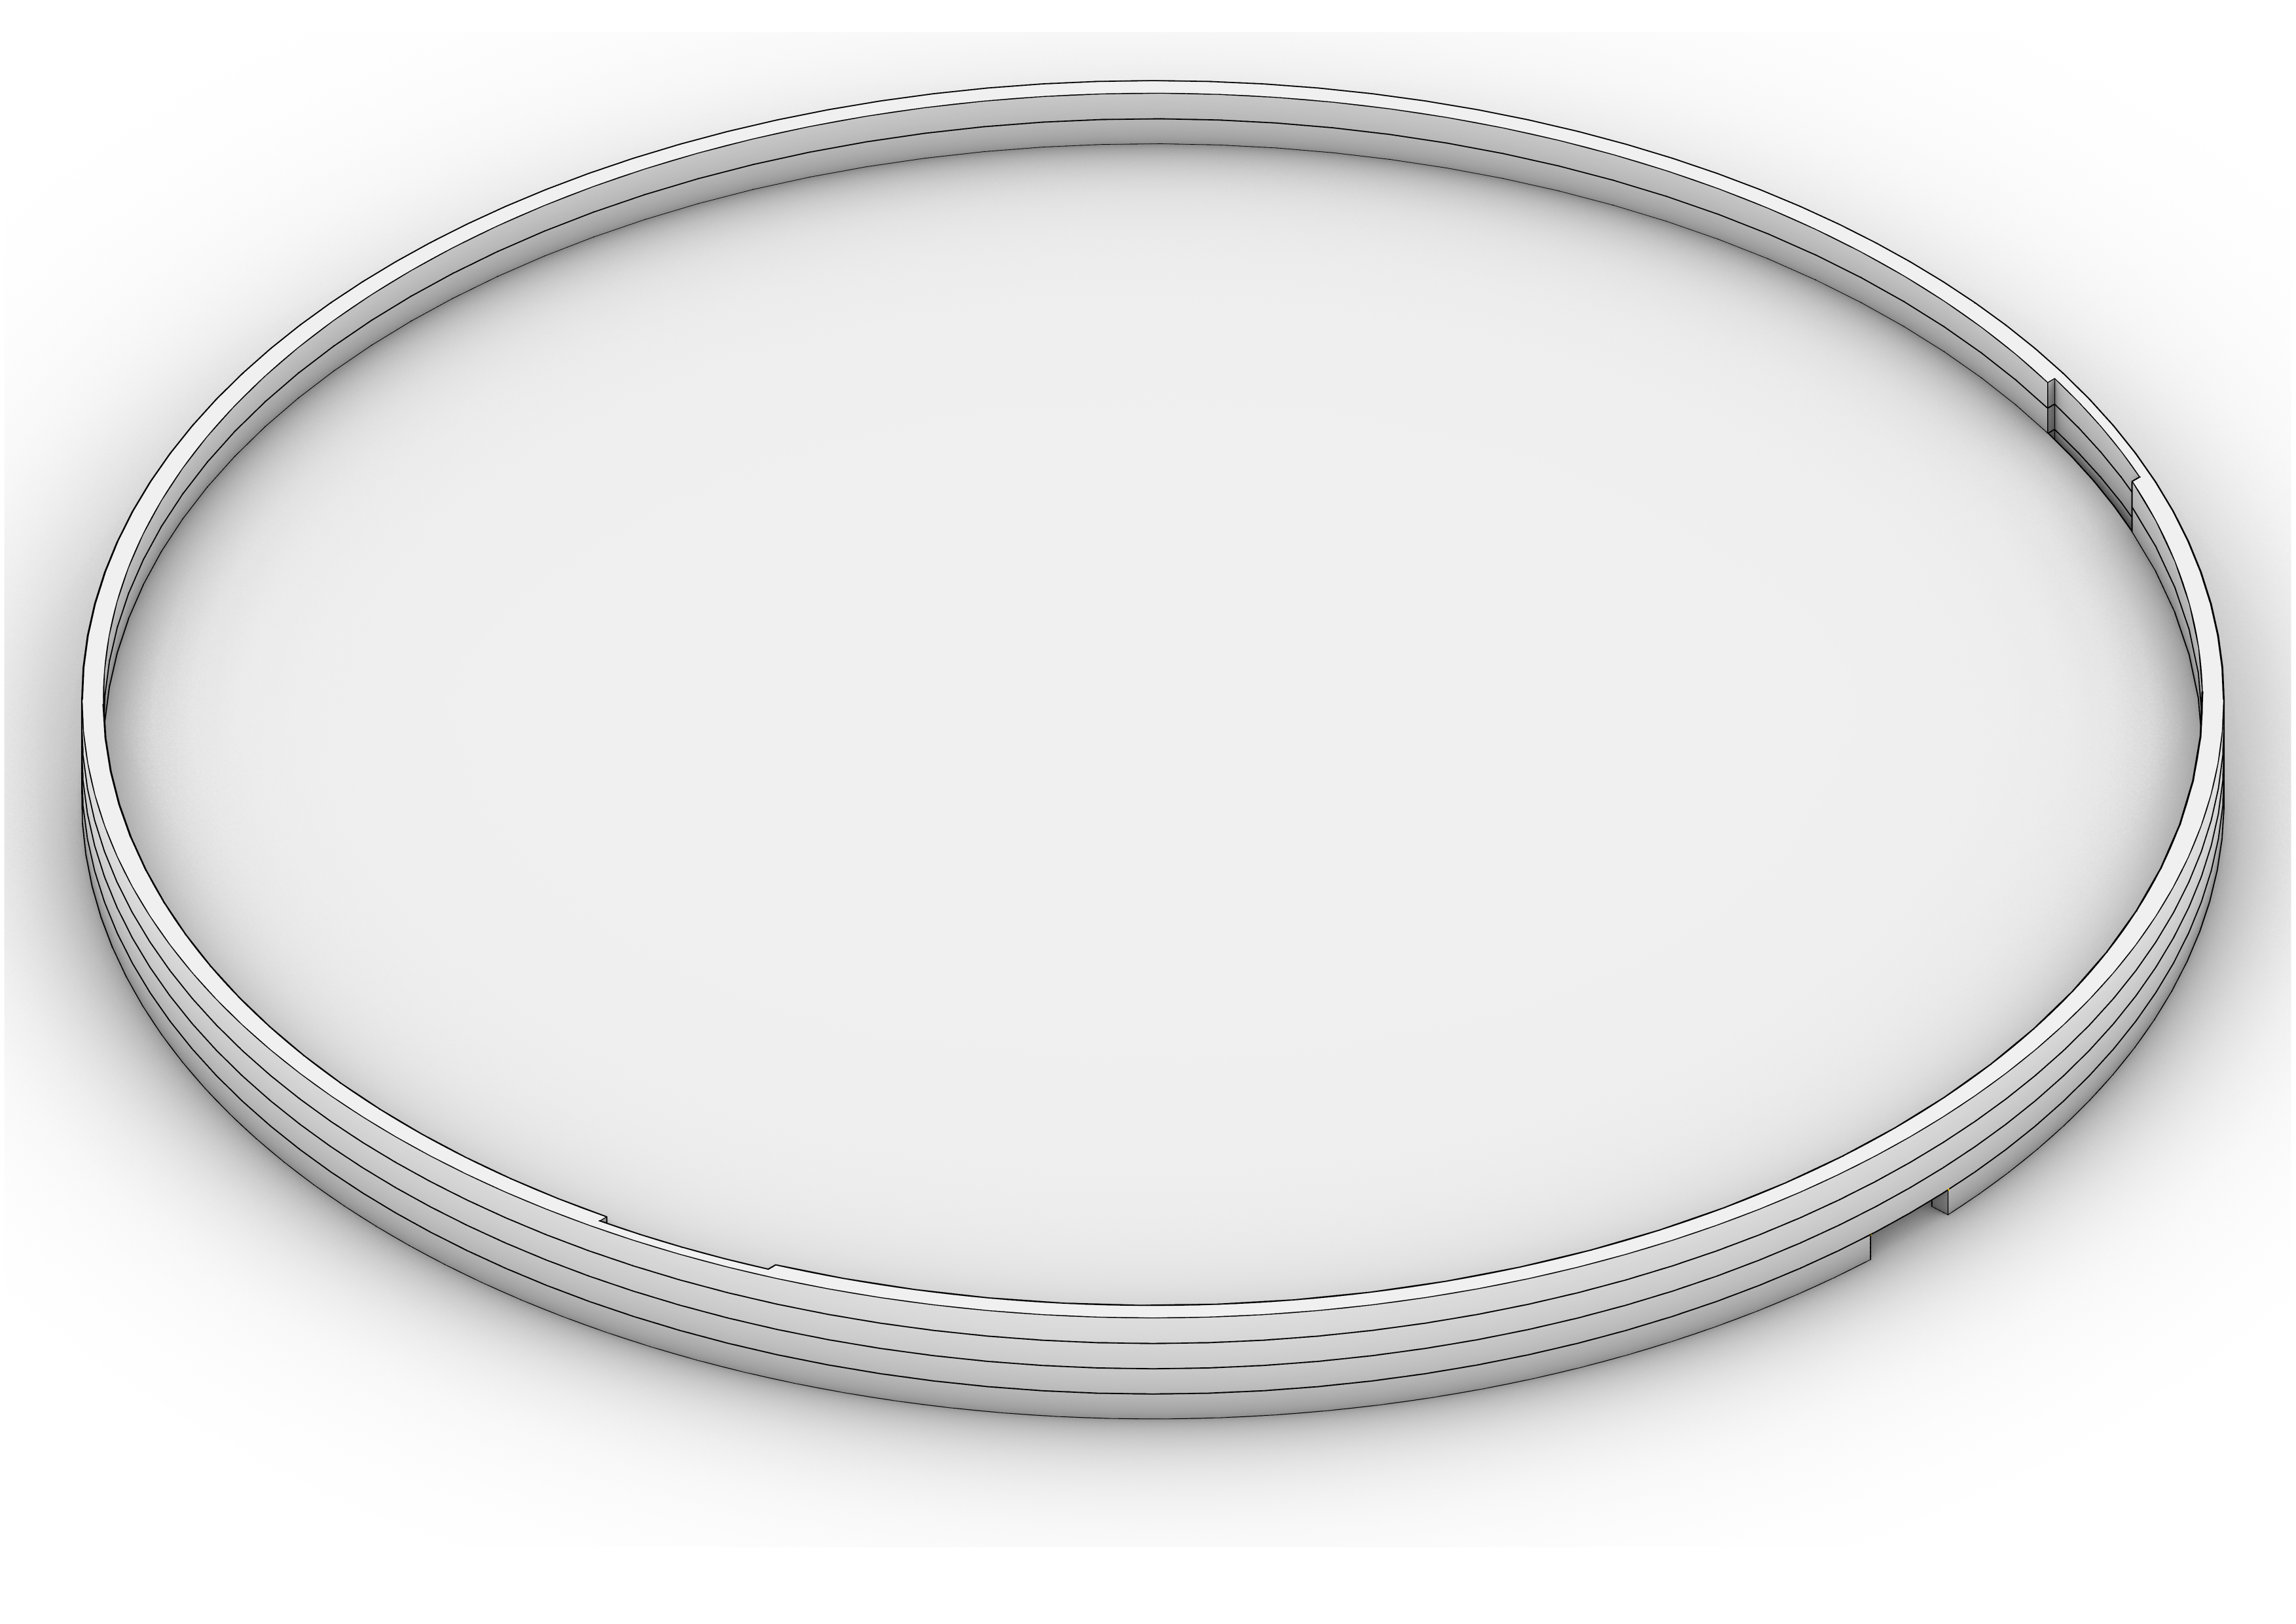
\includegraphics[width=.95\linewidth]{Images/base SG.png}
       \\{Singapore}
         \label{base sg}
    \end{minipage}
    \hfill
    \begin{minipage}{0.48\linewidth}
         \centering
        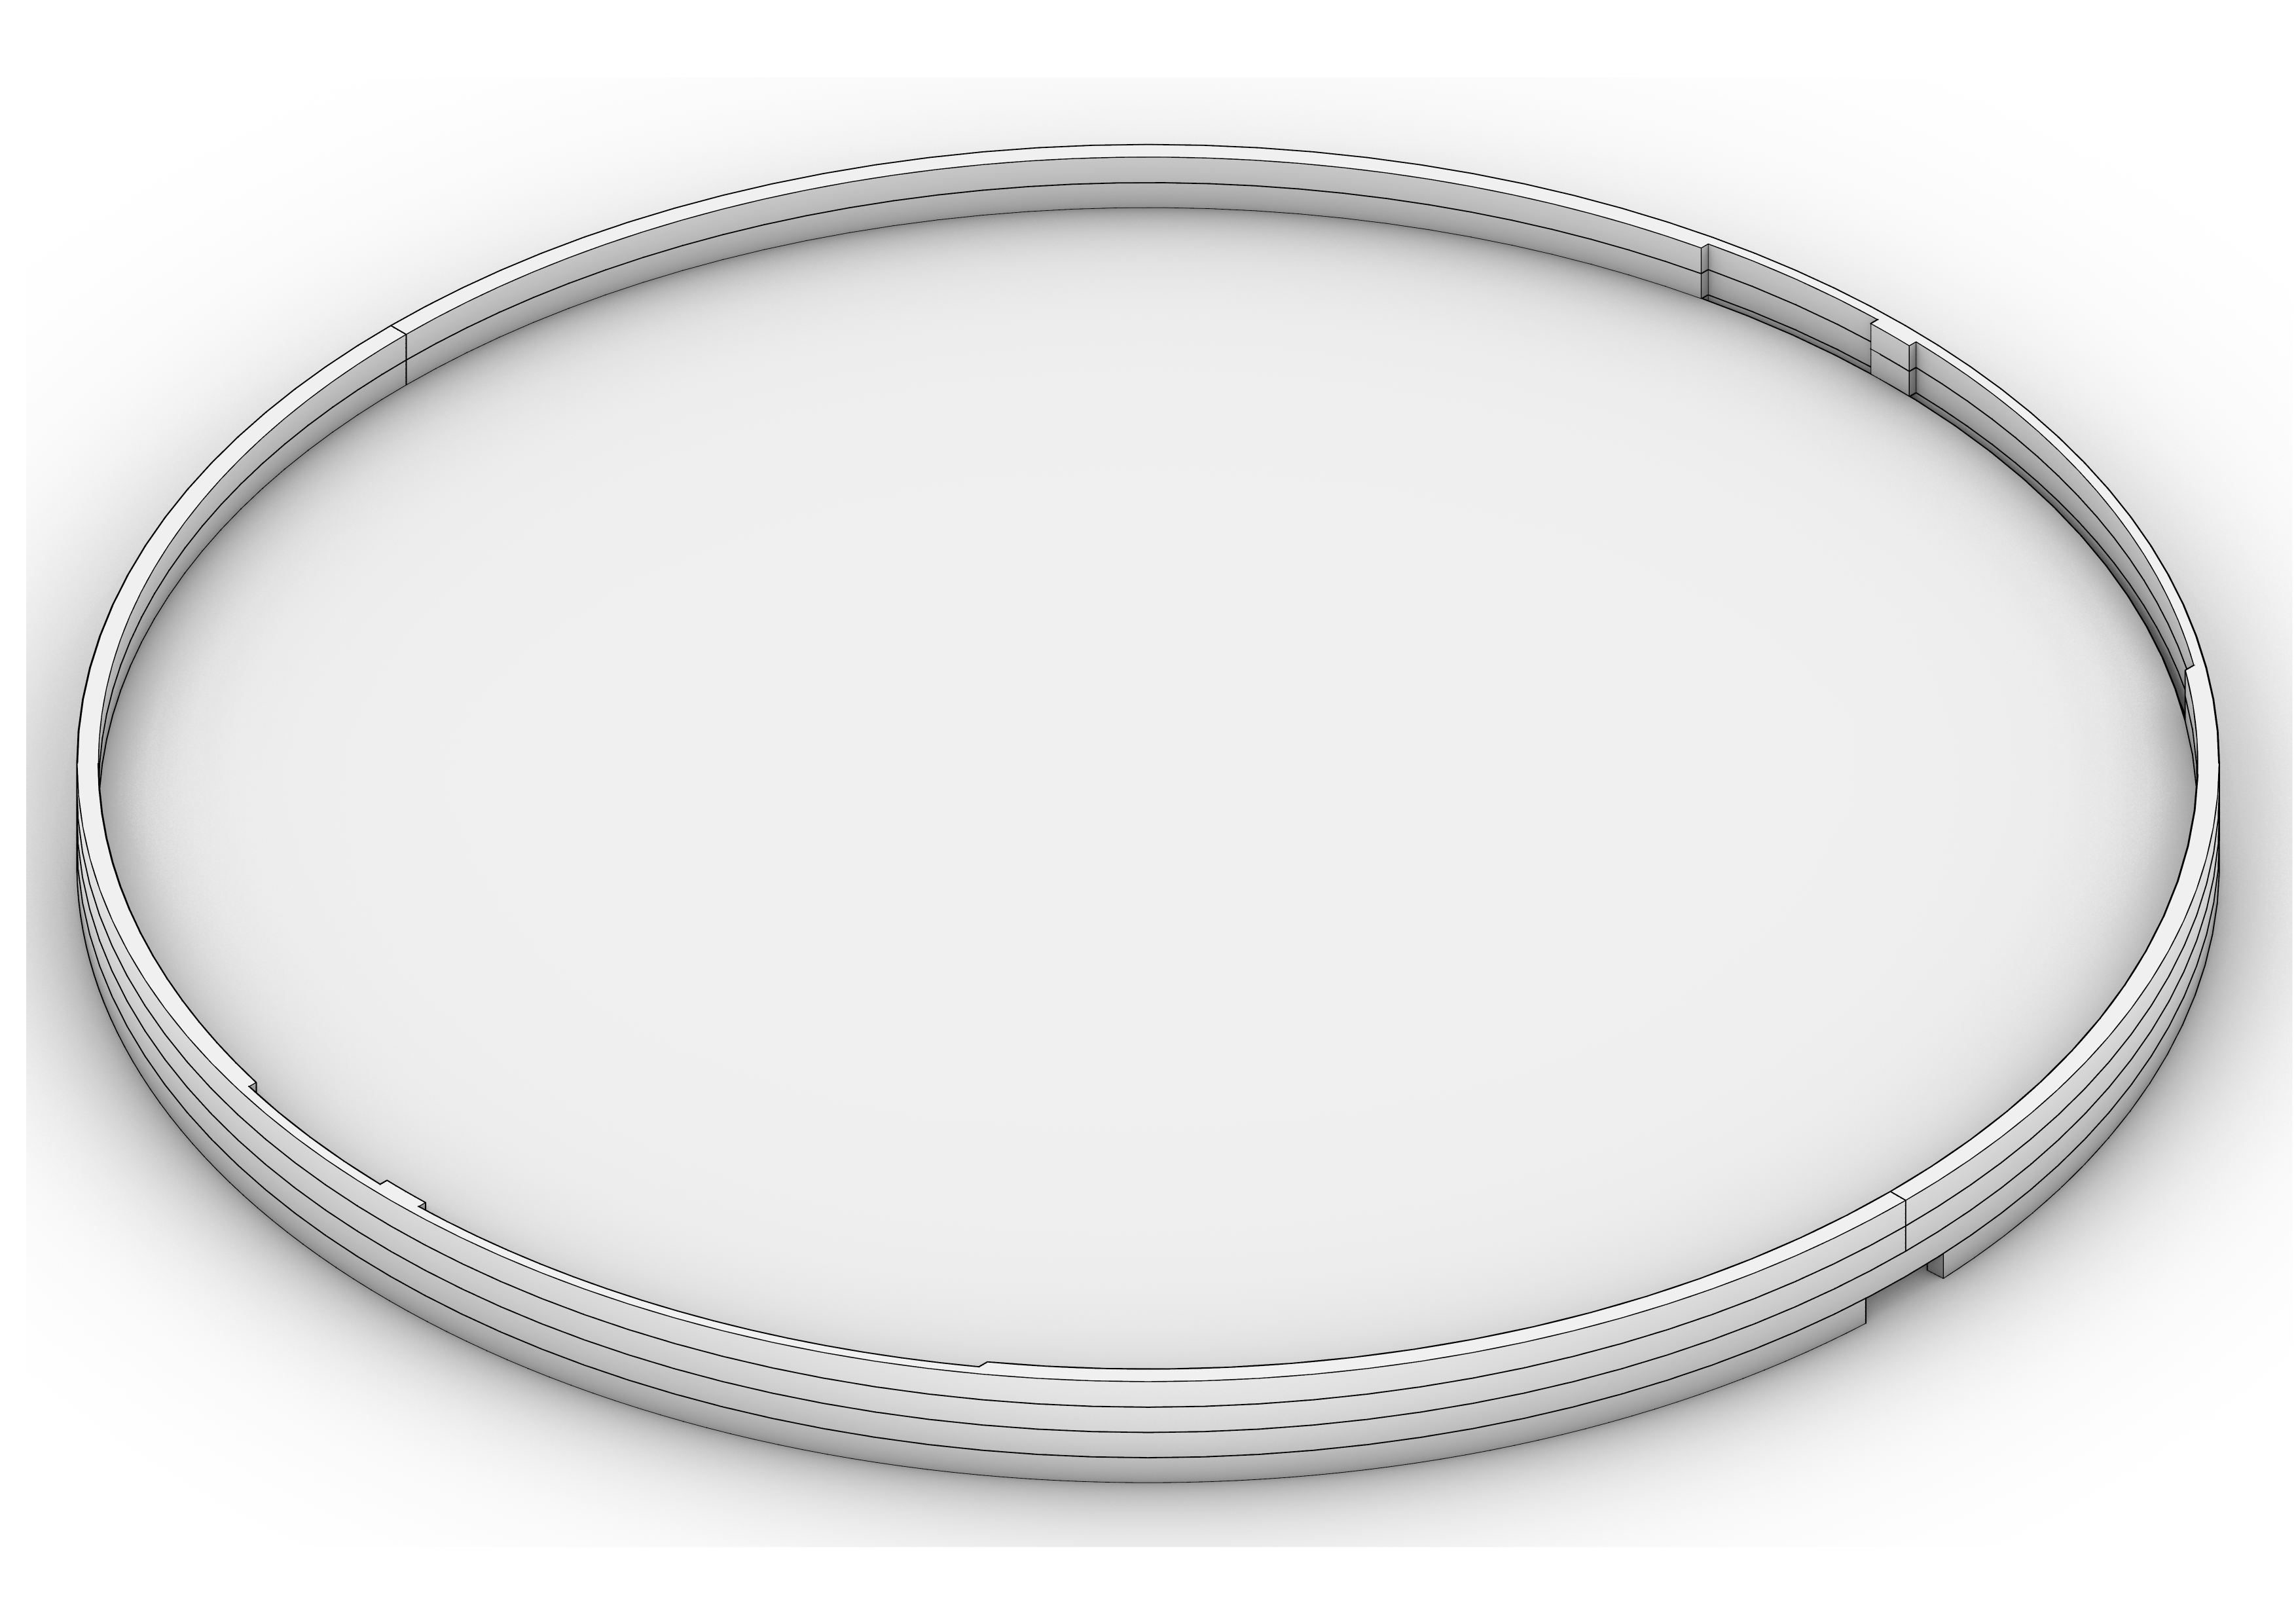
\includegraphics[width=.95\linewidth]{Images/base ZH.png}
       \\{Zurich}
        \label{base zh}
    \end{minipage}
    \captionof{figure}{3D plan of the assambled base}
    \label{base}
\vspace{1cm}
     \begin{minipage}{0.48\linewidth}
        \centering
        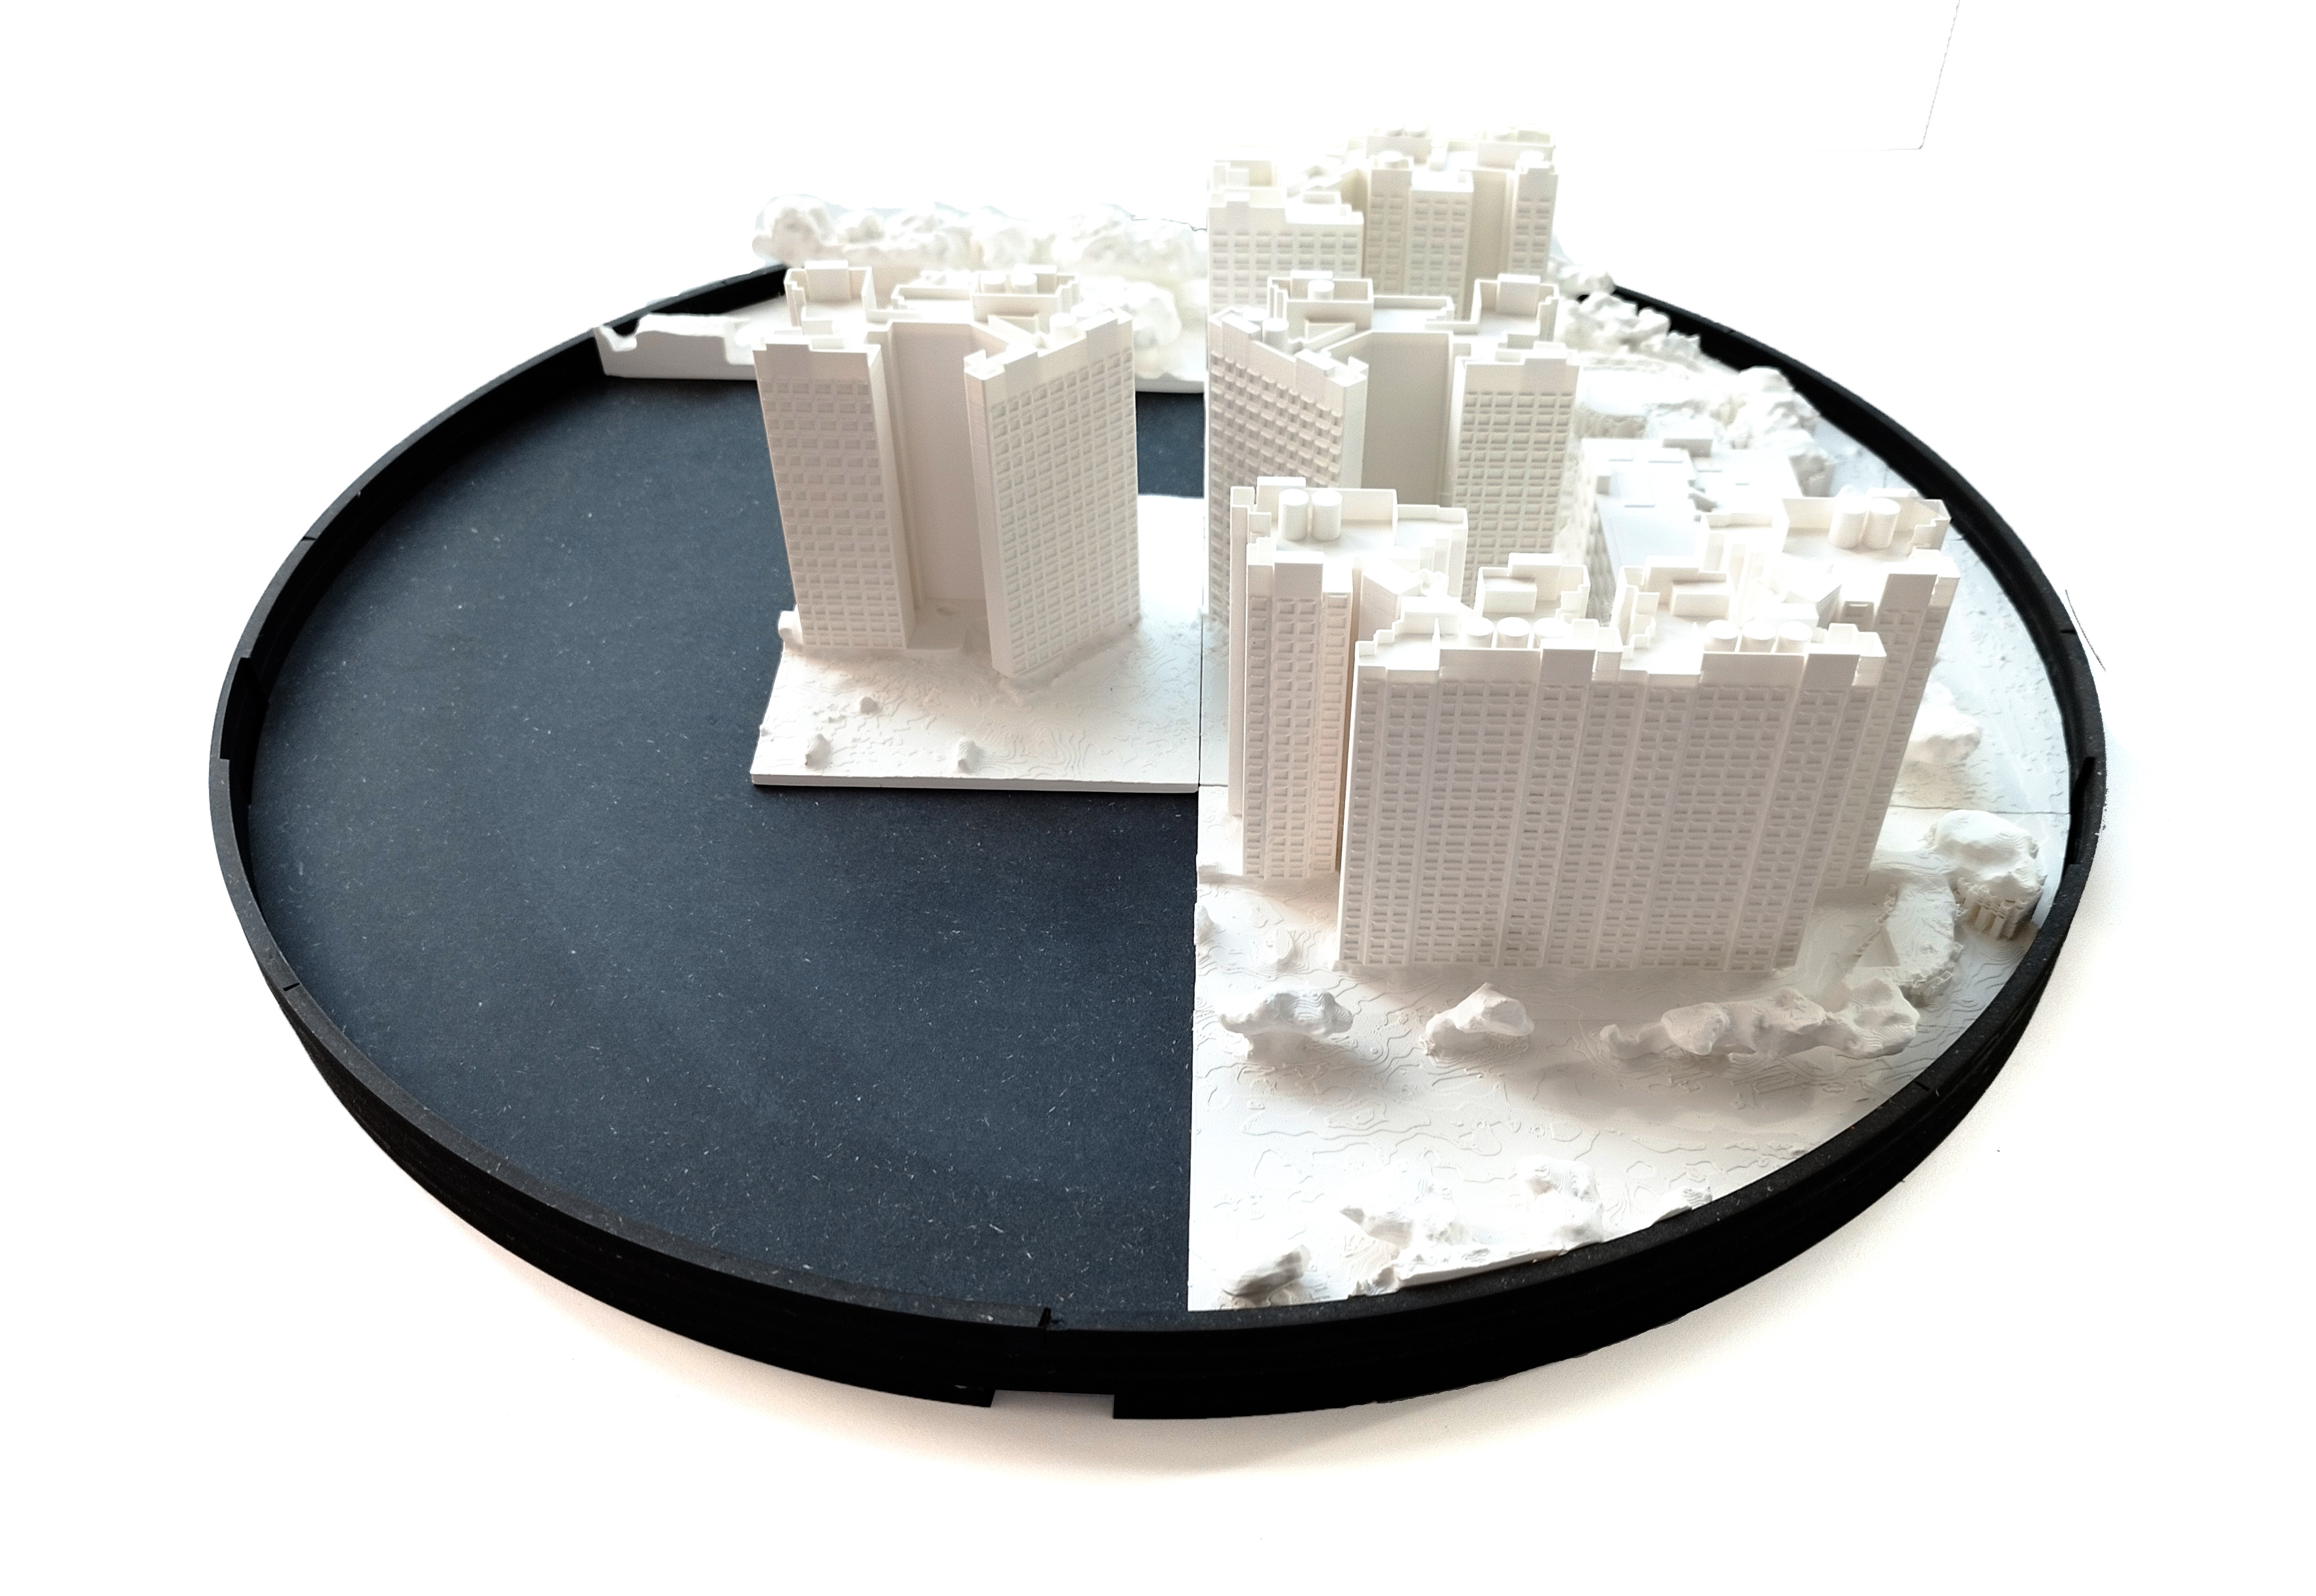
\includegraphics[width=.95\linewidth]{Images/Model SG_1.jpg}
       \\{Singapore}
         \label{base sg2}
    \end{minipage}
    \hfill
    \begin{minipage}{0.48\linewidth}
         \centering
        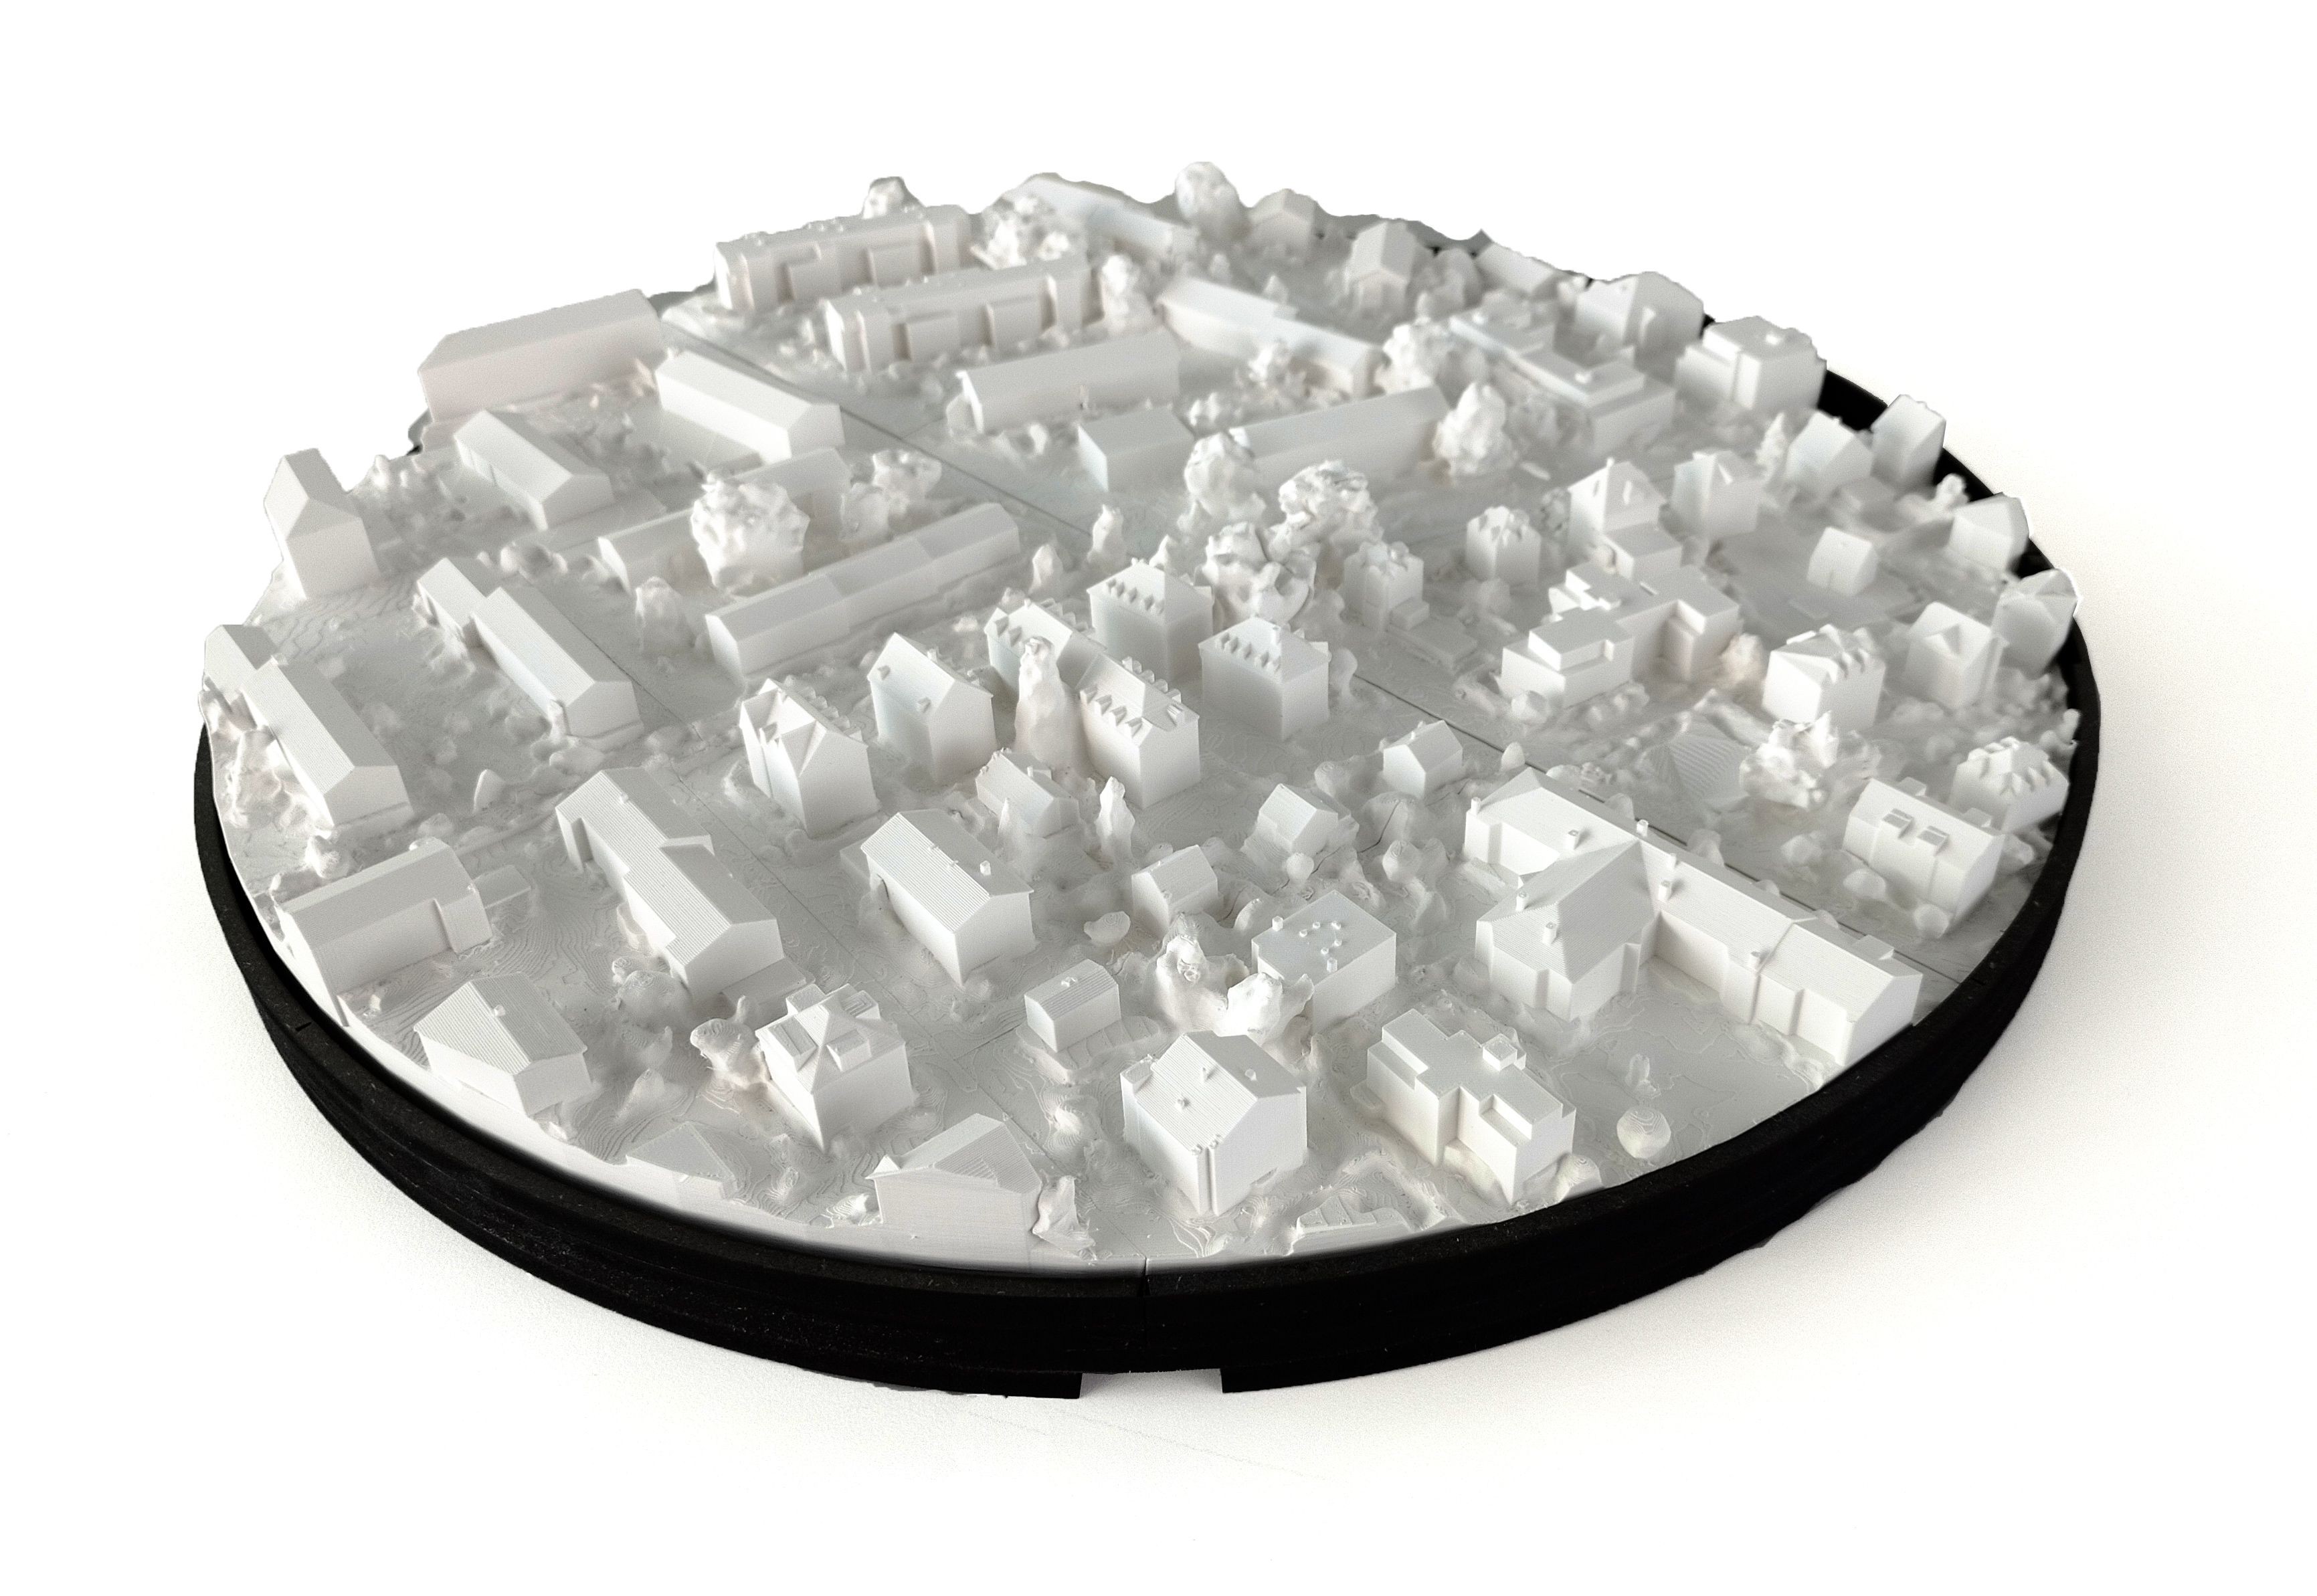
\includegraphics[width=.95\linewidth]{Images/Model ZH_1.jpg}
       \\{Zurich}
        \label{base zh2}
    \end{minipage}
    \captionof{figure}{The finalised glued MDF base}
    \label{baseee}

    \begin{landscape}
        \begin{figure}[H]
        \centering
        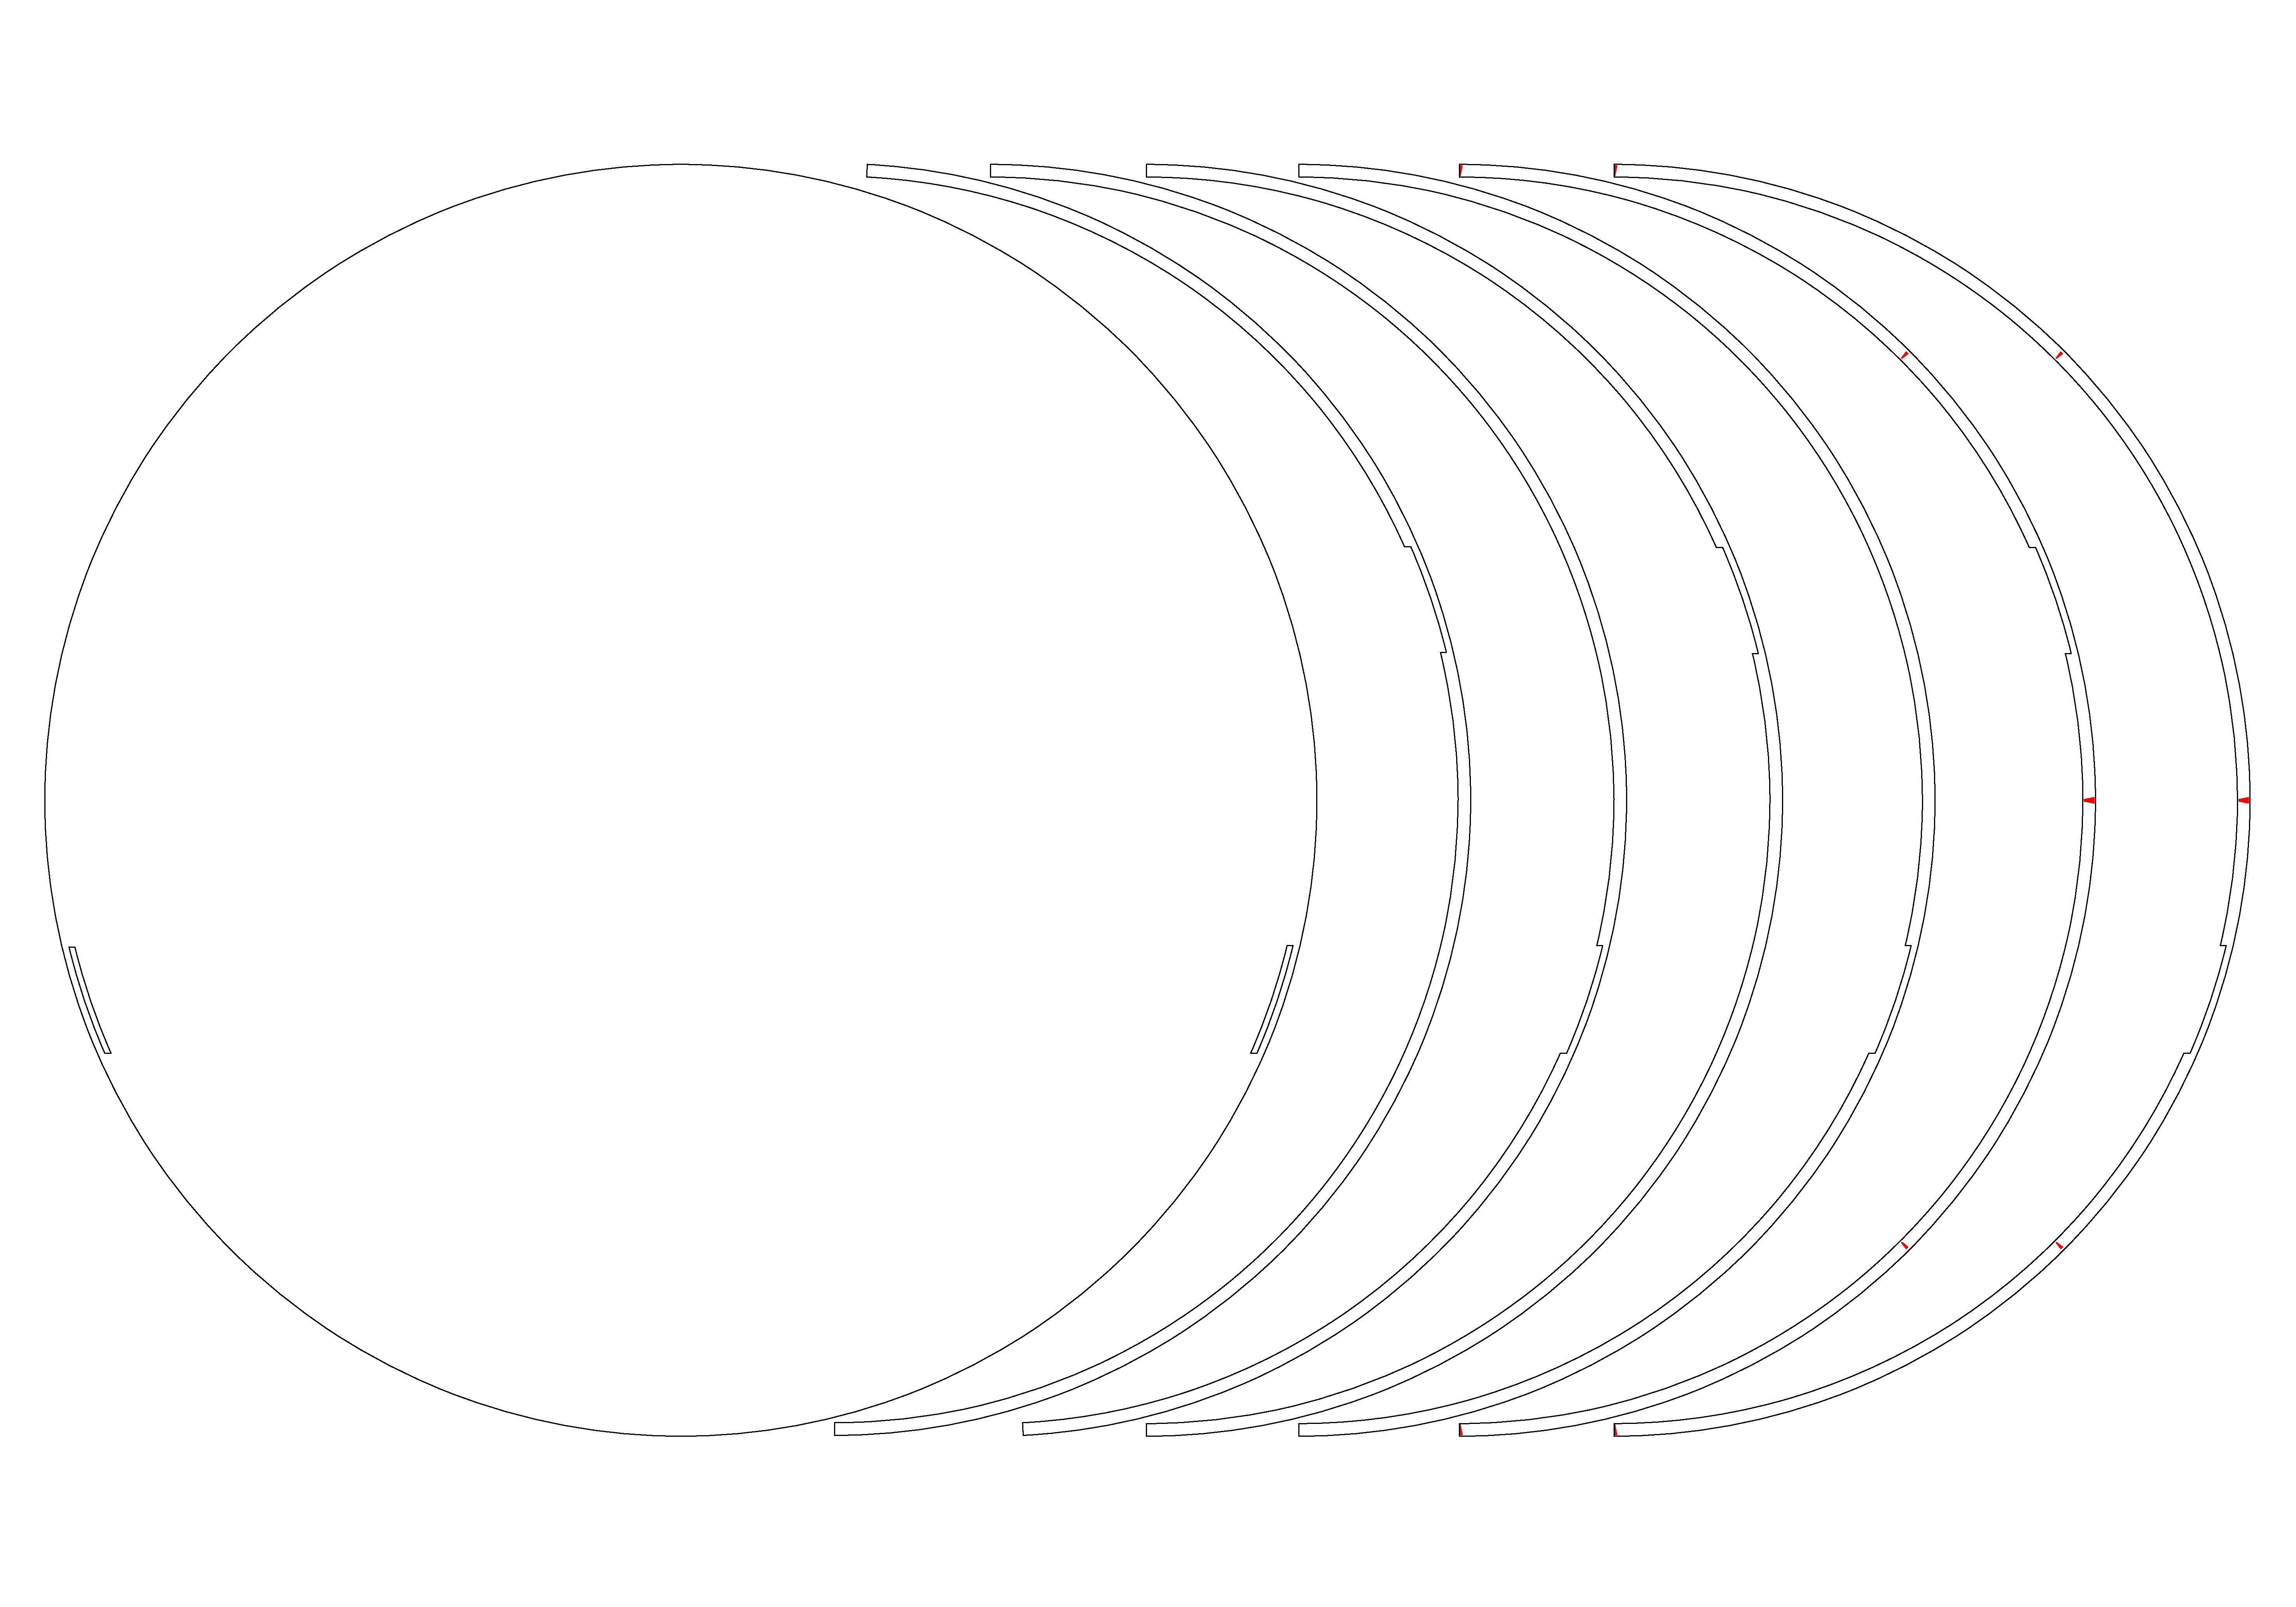
\includegraphics[width=.95\linewidth]{Images/cut sg.pdf}
       \caption{Cut scheme for the MDF laser cutting Singapore}
         \label{cuuuut2}
    \end{figure}
    \begin{figure}[H]
         \centering
        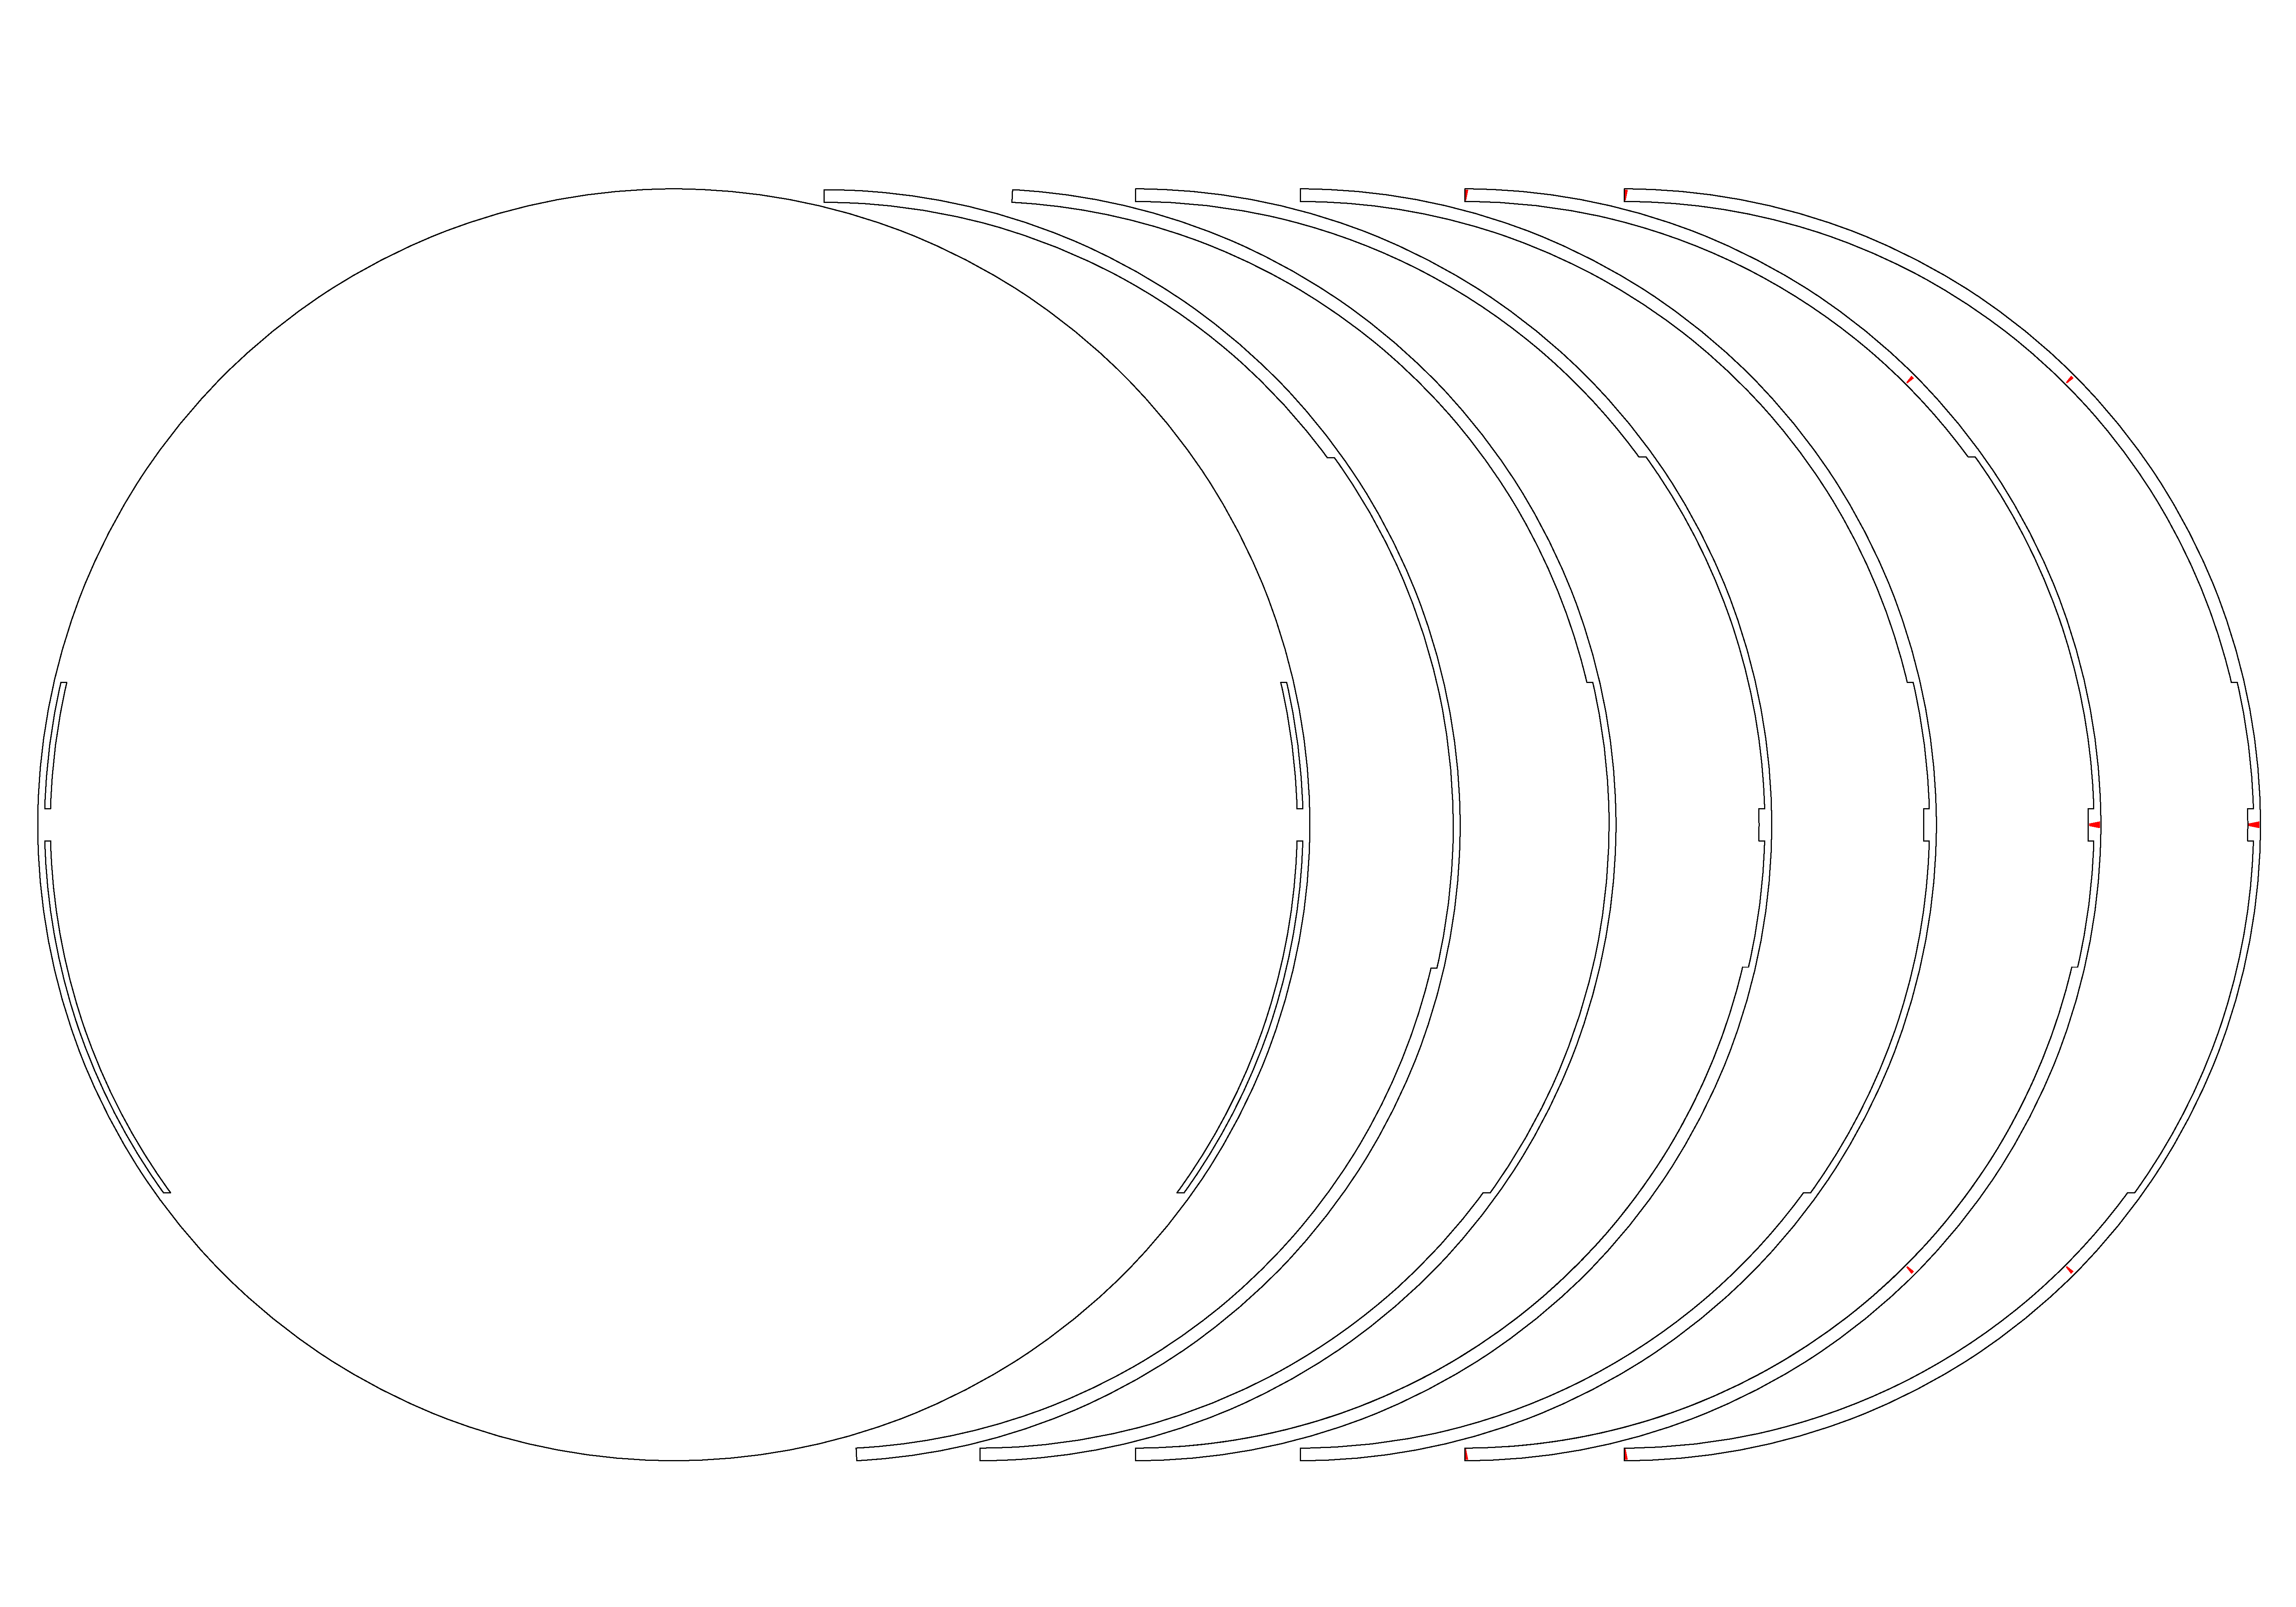
\includegraphics[width=.95\linewidth]{Images/cut zh.pdf}
    \caption{Cut scheme for the MDF laser cutting Zurich}
    \label{cuuuut}
    \end{figure}
    \end{landscape}
    \begin{multicols}{2}
    [
        \subsection{The sunpath and the analemmas}
        \label{sunpa}
    ]
    The final representation of the sun path consists of two bent aluminum profiles marking the paths of the two solstices. They give stability to the whole system and act as mounting rails for the Analemmas which contain the LED lights. \\
    \\
    As shown in \textit{Section} \ref{ana} there has been some prototyping with differently shaped analemma housings. The final housing was produced in a transparent PLA filament. The final design consists of a housing with mounting latches (cf. \textit{Figure} \ref{partshousing}), which were fixed to the metal profiles attached to the base using glue (screwing them would also have been possible, as the latches have a hole prepared for a screw). The LED lights were soldered together with cables corresponding in length with the distances of the holes in the housing. After soldering, the LED lights were mounted inside the base using a double sided transparent scotch tape placed in the indent marking the LEDs position (cf. \textit{Figure} \ref{partshousing}). The LEDs were then taped down using a regular scotch tape. After the LED lights were mounted inside the base, this base was closed using a lid (\textit{Figure} \ref{partshousing}). The lid was designed to fit tightly into the base such that no adhesive is needed to hold it closed. That way it can be opened at any point in time, if repairs to the LED chain or a disassembly should be necessary. Designing the height of the analemmas very minimal, ensures the leds stay in place, since they are held down by the pressure of the lid. \\
    \\
    For simplicity reason all analemmas have been approximated with the same shape, even though technically this does not correspond with reality. For the Zurich location the six analemmas on the side (first three in the morning and second 3 in the evening needed to be cut, as part of them are located below the horizon (cf. \textit{Figure} \ref{cut})
    \end{multicols}
       
 
     \begin{minipage}{0.48\linewidth}
        \centering
        \includegraphics[width=.85\linewidth]{Images/anallemma.png}
       \\
       {Detail plan of the Analemma housing}
         \label{partshousing}
    \end{minipage}
    \hfill
    \begin{minipage}{0.48\linewidth}
         \centering
        \includegraphics[width=.85\linewidth]{Images/cut.png}
        \quad
       \\{Cut housings for Zurich}
        \label{cut}
    \end{minipage}
    \captionof{figure}{CAD plans of the Analemma housings}
    
    \begin{multicols}{2}
    [
    \subsubsection{Cable management}
    ]
    A hole in the base as well as in the lid was was introduced in the final design to run the cables of the LEDs out of the housing. The cables were run along the underneath side of the metal profile, well hidden from views and subsequently through the slits in the base and out of the opening in the front of the base (cf. \textit{Figure} \ref{base} and \ref{final}). Then the cables were routed into the user control box (cf. \textit{Section} \ref{box}) and connected to the respective sources using a system of "WAGO" connectors. (cf. \textit{Section} \ref{elec}).
    \end{multicols}
     \begin{minipage}{0.48\linewidth}
     \begin{figure}[H]
        \centering
        \includegraphics[width=.35\linewidth]{Images/anatop.png}
       \captionof{figure}{Top view of the mounted analemmas)}
         \label{partshousing}
         \end{figure}
    \end{minipage}
    \hfill
    \begin{minipage}{0.48\linewidth}
    \begin{figure}[H]
         \centering
        \includegraphics[width=.54\linewidth]{Images/ana bottom.png}
        \captionof{figure}{Bottom view of the mounted analemmas}
        \label{cut}
        \end{figure}
    \end{minipage}
    
\newpage
 \begin{multicols}{2}
 [
      \subsection{The user experience}
      \label{box}
 ]
 To allow the user to set the desired date and the data set he wants to see, an interface is needed. This will be created using physical turning knobs, as analog input is easier to handle with an Arduino micro controller than dealing with digital input on the serial port. Furthermore, an analog interface is easy to understand and use for almost everyone, as one just has to turn a knob.\\
 \\
 For the aforementioned turning knobs three simple "Drehgeber" were used, which have 24 individual positions each. As a feedback (to see in which position the knob currently is set to) and to give more detailed information about the currently selected data a 4x20line LCD screen is used. To allow for a clear interface and a good cable management all these elements were cased using a plywood box (cf. \textit{Figure} \ref{boxxx}). The plywood box was lasercut and joind using glue and the finger joints. The lid of the box is removable and held in place by a set of screws and nuts in the corners.\\
 \\[.5cm]
 This user interface allows the user to visualize the whole year, the sun path from morning to evening in a specific month or all the positions of the sun in the different months for one specific hour. Furthermore, if month and hours are set, the user can look at one specific LED. No matter what setting the knobs are in, the user is prompted with a minimal and a maximal data value for the currently active LEDs/sun positions. As such, if a user wants they can read out all data value, but can also have a good overview of the data. Basically leaving them optimal control over what is displayed. (cf. \textit{Figure} \ref{controoool}) In addition to the LCD screen a printed legend was mounted, explaining the color code of the different modes, leading to a better distinguish-ability of the different modes and a better understanding of the user about what is shown. Using the same legend for Zurich as well as for Singapore allows cross comparability and might motivate some people to interact with both models trying to compare the different locations.
 \end{multicols}
 \begin{minipage}{0.31\linewidth}
    \centering
    \includegraphics[width=.95\linewidth]{Images/m.jpg}
    \\{one month, all hours}
\end{minipage}
\hfill
\begin{minipage}{0.31\linewidth}
    \centering
    \includegraphics[width=.95\linewidth]{Images/h.jpg}
    \\{all months, one hour}
\end{minipage}
\hfill
\begin{minipage}{0.31\linewidth}
    \centering
    \includegraphics[width=.95\linewidth]{Images/d.jpg}
    \\{one month, one hour}
\end{minipage}
\captionof{figure}{Different possible knob settings}
\label{controoool}
\begin{center}
\begin{minipage}{0.48\linewidth}
         \begin{figure}[H]
        \centering
        \includegraphics[width=.85\linewidth]{Images/box.jpg}
        \caption{The horizontal coordinate system}
        \label{boxxx}
    \end{figure}
\end{minipage}
\end{center}


\begin{landscape}
    \begin{figure}[H]
        \centering
        \includegraphics[width=.75\linewidth,trim={50 50 50 50}]{Images/singapore box.jpg}
        \caption{Cut scheme box Singapore}
    \end{figure}
      
    \begin{figure}[H]
         \centering
            \includegraphics[width=.75\linewidth,trim={50 50 50 50}]{Images/Zurich box.jpg}
        \caption{Cut scheme box Zurich}
    \end{figure}
\end{landscape}
\begin{multicols}{2}
[
    \subsection{The Electronics and the Code}
    \label{elec}
    ]

    The heart of the installation is an Arduino Due. In some first attempts a standard Arduino was used. However, this lead to some errors and turned out to be infeasible due to the lack of enough RAM to drive the LEDs (cf. \textit{Section} \ref{feedback}) and the availability of only two interuptable ports. As each turn of a knob needs to interrupt the code in its execution and register the new state of the knob, each of the three knobs need an interruptable port. Meaning three interuptable ports are needed. The Arduino due solves all the aforementioned problems. Being based on an ARM architecture, it has significantly more RAM and allows to have an interrupt on any of its ports. The LEDS were accessed using the libraries described in \textit{Section} \ref{light}. The LCD mentioned in user experience was programmed using an I2C interface and the "LiquidCrystal I2C" library (which technically is not compatible with the Arduino Due, but worked very well nevertheless). The "Drehgeber" which were used as the turning knobs did not need any library, as they are just an electric circuit connecting three contacts in different combinations depending on the turn direction. These were implemented with a custom made code. The details about a possible cabling scheme of the Arduino can be seen below. The respective program code can be found in the \textit{Annex A} and \textit{Annex B}.\\
    \\
    To ensure that the dome is always glowing and does not freeze due to a crash, a watchdog and a timer were introduced. The timer is reset every time a knob is turned. Should no knob be turned for about 3min and the timer reaches 9000, the installation will reset to a state were all LEDs are glowing. To randomly get one of the four modes after reset (sun position mode excepted), a random number is generated using a measurement of the signal at one of the analogue ports as a seed for the random function. This was done due to the lack of any better method to generate pseudo random numbers with the Arduino.\\
    \\
    The code is structured the following. There is the setup routine, which initializes all the components, variables and flags. There is the loop function, which is called over and over again. In the loop, the variables "mode", "month" and "hour" are evaluated. The mode variable determines which routine is executed. The month variable determines the bounds forwarded to the respective routine (depending on the mode set) The chosen routine uses the "hour" and the bounds to set the LED lights to the respective information and requests the print routines to print the respective values on the display. As a last task, the loop checks, if the knobs were turned in the meantime (meaning the routine was interrupted). It reads the new state of the variables "mode", "month" and "hour" and then starts over.\\
    \\
    If a knob is turned, when the loop is currently busy with another action than reading the knob state, the code will be interrupted, the variables "mode", "month" and "hour" will be set accordingly and the code continues where it was interrupted.\\
    \\
    The hourly data was aggregated to "monthly" averages for every individual hour of the day and then formatted as arrays per hour in the from of\\ "{\tiny$mode\_hour[Jan, Feb, Mar, Apr, May, Jun, Jul, Aug, Sep, Oct, Nov, Dec]$}"\\ As this is the most common order of the months from simulation outputs. However, the first LED in the LED chain is the led representing the winter solestice, meaning 21$^{st}$ of December. Thus, in the code creating the control Data for the LEDs, the whole array was shifted by one position such that it corresponds with the physical position of the LEDs.\\
    \\
    The color schemes for the different modes were created by creating the RGBW values with an affine function using the data values and the minimal and maximal data values of each data set. The affine function parameters were tuned in a way, such that the color scheme has an as good separation of the different colors as possible without loosing the cross comperability between the Zurich and the Singapore model.\\
    \\
    For a more detailed insight consult the flow diagram below (cf. \textit{Figure} \ref{flowcode} and the respective code sections in the \textit{Annex A and Annex B}.
    
\end{multicols}
\begin{landscape}
\begin{figure}[H]
        \centering
        \includegraphics[width=.9\linewidth, trim={50 50 50 50}]{Images/plan software.pdf}
        \caption{Connection Scheme Zurich}
        \label{flowcode}
    \end{figure}

 \begin{figure}[H]
        \centering
        \includegraphics[width=\linewidth, trim={50 50 50 50}]{Images/schaltplan ZH.pdf}
        \caption{Connection Scheme Zurich}
        \label{scheme ZH}
    \end{figure}

     \begin{figure}[H]
        \centering
        \includegraphics[width=\linewidth, trim={50 50 50 50}]{Images/schaltplan SG.pdf}
        \caption{Connection Scheme Singapore}
        \label{scheme SG}
    \end{figure}

\end{landscape}

\section{The final result}
The final model was displayed during the "Future City Labaratory Conference" in the main building of ETH Zurich (cf. \textit{Figure} \ref{hg}). And can now be seen until May 2024 in the H-floor of the HIL on the Hönggerberg Campus. As far as I can tell, the model was received very good during the exhibition period and in my opinion the images below say it all.

\begin{minipage}{0.48\linewidth}
         \begin{figure}[H]
        \centering
        \includegraphics[width=\linewidth]{Images/d1.jpg}
     
    
    \end{figure}
    \end{minipage}
    \hfill
    \begin{minipage}{0.48\linewidth}
         \begin{figure}[H]
        \centering
        \includegraphics[width=\linewidth]{Images/d2.jpg}
   

    \end{figure}
\end{minipage}
\begin{center}
\begin{minipage}{0.48\linewidth}
         \begin{figure}[H]
        \centering
        \includegraphics[width=\linewidth]{Images/dr.jpg}
    \end{figure}
\end{minipage}
\captionof{figure}{The domes in different combinations of modes}
\end{center}
\begin{landscape}
    

\begin{minipage}{0.48\linewidth}
         \begin{figure}[H]
        \centering
        \includegraphics[width=\linewidth]{Images/n1.jpg}
        \captionof{figure}{Final model Zurich}
        \label{fin1}
    \end{figure}
    \end{minipage}
    \hfill
    \begin{minipage}{0.48\linewidth}
         \begin{figure}[H]
        \centering
        \includegraphics[width=\linewidth]{Images/n2.jpg}
        \captionof{figure}{Final model Singapore}
        \label{fin2}
    \end{figure}
\end{minipage}
\end{landscape}
\begin{minipage}{0.48\linewidth}
         \begin{figure}[H]
        \centering
        \includegraphics[width=\linewidth]{Images/1.jpg}
        \captionof{figure}{The exhibition setup in ETH main building}
        \label{hg}
    \end{figure}
    \end{minipage}
    \hfill
    \begin{minipage}{0.48\linewidth}
         \begin{figure}[H]
        \centering
        \includegraphics[width=\linewidth]{Images/2.jpg}
        \captionof{figure}{Exhibition in progress}
    \end{figure}
\end{minipage}
\begin{minipage}{0.48\linewidth}
         \begin{figure}[H]
        \centering
        \includegraphics[width=\linewidth]{Images/3.jpg}
        \captionof{figure}{Exhibition in progress}
    \end{figure}
    \end{minipage}
    \hfill
    \begin{minipage}{0.48\linewidth}
         \begin{figure}[H]
        \centering
        \includegraphics[width=\linewidth]{Images/5.jpg}
        \captionof{figure}{Model Zurich in white spotlight}
  
    \end{figure}
\end{minipage}
\begin{minipage}{0.48\linewidth}
         \begin{figure}[H]
        \centering
        \includegraphics[width=\linewidth]{Images/f1.jpg}
        \captionof{figure}{Grid Emission Mode}
    
    \end{figure}
    \end{minipage}
    \hfill
    \begin{minipage}{0.48\linewidth}
         \begin{figure}[H]
        \centering
        \includegraphics[width=\linewidth]{Images/f2.jpg}
        \captionof{figure}{Sun position mode}
    
    \end{figure}
\end{minipage}
\newpage

\begin{minipage}{0.48\linewidth}
         \begin{figure}[H]
        \centering
        \includegraphics[width=.9\linewidth, angle =180]{Images/e1.jpg}
        \captionof{figure}{Heating/Cooling demand mode}

    \end{figure}
    \end{minipage}
    \hfill
    \begin{minipage}{0.48\linewidth}
         \begin{figure}[H]
        \centering
        \includegraphics[width=.9\linewidth, angle =180]{Images/e2.jpg}
        \caption{Solar irradiation mode}
 
    \end{figure}
\end{minipage}

\begin{minipage}{0.48\linewidth}
         \begin{figure}[H]
        \centering
        \includegraphics[width=.9\linewidth]{Images/e3.jpg}
        \captionof{figure}{Sun position mode}

    \end{figure}
    \end{minipage}
    \hfill
    \begin{minipage}{0.48\linewidth}
         \begin{figure}[H]
        \centering
        \includegraphics[width=.9\linewidth]{Images/e4.jpg}
        \captionof{figure}{Grid emissions mode}
    
    \end{figure}
\end{minipage}
\newpage
\section*{$\;$}
\noindent\hrulefill $\;\;\;\;${\Large \textbf{References}}$\;\;\;$ \noindent\hrulefill
\phantomsection
\AtNextBibliography{\small}
\addcontentsline{toc}{section}{References}
\printbibliography[title=$\;$]
\newpage
\section*{$\;$}
\noindent\hrulefill $\;\;\;\;${\Large \textbf{Annex}}$\;\;\;$ \noindent\hrulefill\\[1.6cm]
\phantomsection
\addcontentsline{toc}{section}{Annex}
\label{Annex}
\subsection*{Annex A: Code for the Singapore sun path visualisation}
\label{anA}
\begin{lstlisting}[basicstyle=\tiny,style=CStyle]
#include <Adafruit_NeoPixel.h>
#include <PGMWrap.h>
#include <LiquidCrystal_I2C.h>

LiquidCrystal_I2C lcd(0x27,20,4);


#define PIX_8 12
#define PIX_9 11
#define PIX_10 10
#define PIX_11 9
#define PIX_12 8
#define PIX_13 7
#define PIX_14 6
#define PIX_15 5
#define PIX_16 4
#define PIX_17 3
#define PIX_18 2


#define CONT_1 20
#define CONT_2 21
#define CONT_3 22

#define ENC_mode_A 24
#define ENC_mode_B 25
#define ENC_month_A 28
#define ENC_month_B 29
#define ENC_hour_A 32
#define ENC_hour_B 33

#define NUMPIXELS 12
#define DELAYVAL 100

//initialize pixles for the analemmas

Adafruit_NeoPixel pixels_8(NUMPIXELS, PIX_8, NEO_GRBW + NEO_KHZ800);
Adafruit_NeoPixel pixels_9(NUMPIXELS, PIX_9, NEO_GRBW + NEO_KHZ800);
Adafruit_NeoPixel pixels_10(NUMPIXELS, PIX_10, NEO_GRBW + NEO_KHZ800);
Adafruit_NeoPixel pixels_11(NUMPIXELS, PIX_11, NEO_GRBW + NEO_KHZ800);
Adafruit_NeoPixel pixels_12(NUMPIXELS, PIX_12, NEO_GRBW + NEO_KHZ800);
Adafruit_NeoPixel pixels_13(NUMPIXELS, PIX_13, NEO_GRBW + NEO_KHZ800);
Adafruit_NeoPixel pixels_14(NUMPIXELS, PIX_14, NEO_GRBW + NEO_KHZ800);
Adafruit_NeoPixel pixels_15(NUMPIXELS, PIX_15, NEO_GRBW + NEO_KHZ800);
Adafruit_NeoPixel pixels_16(NUMPIXELS, PIX_16, NEO_GRBW + NEO_KHZ800);
Adafruit_NeoPixel pixels_17(NUMPIXELS, PIX_17, NEO_GRBW + NEO_KHZ800);
Adafruit_NeoPixel pixels_18(NUMPIXELS, PIX_18, NEO_GRBW + NEO_KHZ800);
//initialize pixles for the control panel
Adafruit_NeoPixel control_1(NUMPIXELS, CONT_1, NEO_GRBW + NEO_KHZ800);
Adafruit_NeoPixel control_2(NUMPIXELS, CONT_2, NEO_GRBW + NEO_KHZ800);
Adafruit_NeoPixel control_3(NUMPIXELS, CONT_3, NEO_GRBW + NEO_KHZ800);



String unit_temp="C";
String unit_grid="kgCO2/kWh";
String unit_ghi="W/m2";
String unit_dema="kWh";
float temp_array[]={0,0,0,0,0,0,0,0,0,0,0};
volatile int mode=0;
volatile int month=12;
volatile int hour=11;
float minValue;
float maxValue;
int lower_b;
int upper_b;
int period=200;
int time_now;
int encoderPINA_mode = ENC_mode_A;
int encoderPINB_mode = ENC_mode_B;
int encoderPos_mode = 0;
int encoderPINALast_mode = LOW;
int encoderPINANow_mode = LOW;
int encoderPINA_month = ENC_month_A;
int encoderPINB_month = ENC_month_B;
int encoderPos_month = 0;
int encoderPINALast_month = LOW;
int encoderPINANow_month = LOW;
int encoderPINA_hour = ENC_hour_A;
int encoderPINB_hour = ENC_hour_B;
int encoderPos_hour = 0;
int encoderPINALast_hour = LOW;
int encoderPINANow_hour = LOW;
int a;
int aa;

// SINGAPORE GRID EMISSIONS
float avggrid_8[]={488,488,488,489,487,488,487,487,488,487,488,489};
float avggrid_9[]={492,491,492,492,492,492,492,491,493,492,492,492};
float avggrid_10[]={495,494,495,495,495,494,495,494,497,495,494,495};
float avggrid_11[]={496,495,496,496,495,495,497,495,497,496,494,496};
float avggrid_12[]={496,495,497,496,496,495,497,496,498,496,496,496};
float avggrid_13[]={496,495,497,496,496,495,497,496,498,496,496,496};
float avggrid_14[]={497,495,497,496,496,495,497,496,497,497,495,496};
float avggrid_15[]={497,496,497,497,496,496,498,496,497,497,496,496};
float avggrid_16[]={497,496,498,497,496,496,498,496,497,497,496,497};
float avggrid_17[]={497,496,498,497,496,496,498,496,497,497,496,497};
float avggrid_18[]={498,496,498,497,496,496,498,496,497,497,496,497};
float b_grid=0;
float max_grid=498;
float min_grid=300;
float max_grid_si=498;
float min_grid_si=487;

// SINGAPORE DEMAND


float avgdema_8[]={-279,-324,-716,-854,-1073,-925,-768,-842,-1003,-1052,-670,-498};
float avgdema_9[]={-770,-850,-942,-994,-1112,-999,-928,-966,-1055,-1025,-998,-862};
float avgdema_10[]={-875,-857,-817,-935,-1002,-937,-861,-827,-941,-931,-827,-802};
float avgdema_11[]={-1086,-1085,-1192,-1342,-1445,-1317,-1249,-1243,-1369,-1316,-1227,-1131};
float avgdema_12[]={-1432,-1448,-1535,-1735,-1824,-1670,-1596,-1610,-1746,-1685,-1630,-1459};
float avgdema_13[]={-1436,-1496,-1567,-1710,-1809,-1663,-1578,-1600,-1700,-1680,-1562,-1470};
float avgdema_14[]={-1058,-1164,-1223,-1292,-1386,-1237,-1173,-1180,-1286,-1271,-1160,-1052};
float avgdema_15[]={-829,-936,-1019,-1039,-1127,-995,-921,-942,-1048,-1011,-897,-798};
float avgdema_16[]={-755,-898,-939,-959,-1020,-900,-830,-860,-918,-922,-792,-723};
float avgdema_17[]={-958,-1023,-1053,-1129,-1198,-1074,-989,-1036,-1065,-1064,-926,-867};
float avgdema_18[]={-1839,-1871,-1911,-2055,-2158,-2050,-1935,-1972,-2004,-2006,-1827,-1748};
float g_dema=20;
float max_dema=-279;
float min_dema=-2383;
float max_dema_si=-279;
float min_dema_si=-2383;


// SINGAPORE GHI

float avgghi_8[]={161,162,174,179,189,170,173,177,213,229,182,162};
float avgghi_9[]={313,347,356,327,354,312,318,310,383,406,312,328};
float avgghi_10[]={495,518,529,467,492,476,450,437,508,537,421,456};
float avgghi_11[]={588,594,616,552,514,555,534,513,579,583,494,527};
float avgghi_12[]={646,717,700,639,635,589,582,576,638,609,537,520};
float avgghi_13[]={645,728,698,696,603,598,564,592,629,572,576,569};
float avgghi_14[]={604,693,640,626,538,539,540,587,565,512,494,494};
float avgghi_15[]={509,601,559,494,457,458,498,536,445,421,405,384};
float avgghi_16[]={390,429,413,361,327,350,392,409,322,282,305,294};
float avgghi_17[]={224,267,243,218,184,195,235,233,181,150,144,168};
float avgghi_18[]={80,103,81,69,50,62,82,73,32,12,10,27};
float g_ghi=200;
float max_ghi=728;
float min_ghi=1;
float max_ghi_si=728;
float min_ghi_si=1;


// SINGAPORE TEMP

float avgtemp_8[]={25,25,25,25,26,26,26,26,25,26,25,25};
float avgtemp_9[]={25,25,26,26,27,27,27,27,26,27,26,26};
float avgtemp_10[]={26,27,27,27,28,28,28,28,27,28,26,27};
float avgtemp_11[]={27,28,28,28,29,29,29,29,28,29,27,28};
float avgtemp_12[]={28,28,29,29,30,30,29,29,29,30,28,28};
float avgtemp_13[]={29,29,30,30,31,30,30,30,30,30,29,29};
float avgtemp_14[]={29,30,30,30,31,31,30,30,30,31,29,29};
float avgtemp_15[]={29,30,31,31,32,31,31,31,31,31,30,30};
float avgtemp_16[]={29,30,31,31,32,31,31,31,31,31,30,29};
float avgtemp_17[]={29,30,31,31,32,31,31,31,30,31,30,29};
float avgtemp_18[]={29,30,30,30,31,30,30,30,30,30,29,29};
float g_temp=0;
float max_temp=32;
float min_temp=20;
float max_temp_si=32;
float min_temp_si=25;

int r_sun=100;
int g_sun=100;
int b_sun=100;
int w_sun=200;

int reset_timeout=9000;
int counter=0;
int turn_flag=0;

void setup() {
  watchdogSetup();
  watchdogEnable(10000);
  Serial.begin (115200);
  //initialize LCD
  lcd.init();
  Wire.setClock(400000);
  lcd.clear();         
  lcd.backlight(); 
  //initialize Pixels 
  
  pixels_8.begin();
  pixels_9.begin();
  pixels_10.begin();
  pixels_11.begin();
  pixels_12.begin();
  pixels_13.begin();
  pixels_14.begin();
  pixels_15.begin();
  pixels_16.begin();
  pixels_17.begin();
  pixels_18.begin();
  pinMode (encoderPINA_mode, INPUT_PULLUP);
  pinMode (encoderPINB_mode, INPUT_PULLUP);
  pinMode (encoderPINA_month, INPUT_PULLUP);
  pinMode (encoderPINB_month, INPUT_PULLUP);
  pinMode (encoderPINA_hour, INPUT_PULLUP);
  pinMode (encoderPINB_hour, INPUT_PULLUP);
  attachInterrupt(digitalPinToInterrupt(encoderPINA_month), turn_month, CHANGE);
  attachInterrupt(digitalPinToInterrupt(encoderPINA_hour), turn_hour, CHANGE);
  attachInterrupt(digitalPinToInterrupt(encoderPINA_mode), turn_mode, CHANGE);
  randomSeed(analogRead(A2));
  mode=random(0,4);
  print_mode();
  print_month();
  print_hour();
  // put your setup code here, to run once:

}


void loop() {
  watchdogReset();
  if (turn_flag==1){
    counter=0;
    turn_flag=0;
  }
  if( counter  >= reset_timeout && turn_flag==0 ){ 
    rstc_start_software_reset(RSTC);  
  }
  counter++;

  switch (month) {
  case 0:
  case 1:
  case 2:
  case 3:
  case 4:
  case 5:
  case 6:
  case 7:
  case 8:
  case 9:
  case 10:
  case 11:
  upper_b=month+1;
  lower_b=month;
  break;
  case 12:
  upper_b=12;
  lower_b=0;
  break;
  }
  

  //mode switch
  switch (mode) {
  case 0:
  //clear_pix();   
  temp();
  show();
  break;
  case 1:
  //clear_pix();
  grid();
  show();
  break;
  case 2:
  //clear_pix();
  ghi();
  show();
  break;
  case 3:
  //clear_pix();
  dema();
  show();
  break;
  case 4:
  sunpos();
  show();
  break;
  }

  
  
  turn_mode();
  turn_month();
  turn_hour();
  //clear_pix();
    
   
}
  void ghi(){
    
    for (int i = lower_b; i < upper_b; i++) {
      if(i==0){
        a=11;
      }else{
        a=i-1;
      }
      switch(hour){
        case 0:
          pixels_8.setPixelColor(i,120+125*(avgghi_8[a]-min_ghi)/(max_ghi-min_ghi), g_ghi,170*(max_ghi-avgghi_8[a])/(max_ghi-min_ghi),0);
          break;
        case 1:  
          pixels_9.setPixelColor(i,120+125*(avgghi_9[a]-min_ghi)/(max_ghi-min_ghi), g_ghi,170*(max_ghi-avgghi_9[a])/(max_ghi-min_ghi),0);
          break;
        case 2:
          pixels_10.setPixelColor(i,120+125*(avgghi_10[a]-min_ghi)/(max_ghi-min_ghi), g_ghi,170*(max_ghi-avgghi_10[a])/(max_ghi-min_ghi),0);
          break;
        case 3:
          pixels_11.setPixelColor(i,120+125*(avgghi_11[a]-min_ghi)/(max_ghi-min_ghi), g_ghi,170*(max_ghi-avgghi_11[a])/(max_ghi-min_ghi),0);
          break;
        case 4:
          pixels_12.setPixelColor(i,120+125*(avgghi_12[a]-min_ghi)/(max_ghi-min_ghi), g_ghi,170*(max_ghi-avgghi_12[a])/(max_ghi-min_ghi),0);
          break;
        case 5:
          pixels_13.setPixelColor(i,120+125*(avgghi_13[a]-min_ghi)/(max_ghi-min_ghi), g_ghi,170*(max_ghi-avgghi_13[a])/(max_ghi-min_ghi),0);
          break;
        case 6:  
          pixels_14.setPixelColor(i,120+125*(avgghi_14[a]-min_ghi)/(max_ghi-min_ghi), g_ghi,170*(max_ghi-avgghi_14[a])/(max_ghi-min_ghi),0);
          break;
        case 7:  
          pixels_15.setPixelColor(i,120+125*(avgghi_15[a]-min_ghi)/(max_ghi-min_ghi), g_ghi,170*(max_ghi-avgghi_15[a])/(max_ghi-min_ghi),0);
          break;
        case 8:  
          pixels_16.setPixelColor(i,120+125*(avgghi_16[a]-min_ghi)/(max_ghi-min_ghi), g_ghi,170*(max_ghi-avgghi_16[a])/(max_ghi-min_ghi),0);
          break;
        case 9:
          pixels_17.setPixelColor(i,120+125*(avgghi_17[a]-min_ghi)/(max_ghi-min_ghi), g_ghi,170*(max_ghi-avgghi_17[a])/(max_ghi-min_ghi),0);
          break;
        case 10:
          pixels_18.setPixelColor(i,120+125*(avgghi_18[a]-min_ghi)/(max_ghi-min_ghi), g_ghi,170*(max_ghi-avgghi_18[a])/(max_ghi-min_ghi),0);
          break;
        case 11:
         
          pixels_8.setPixelColor(i,120+125*(avgghi_8[a]-min_ghi)/(max_ghi-min_ghi), g_ghi,170*(max_ghi-avgghi_8[a])/(max_ghi-min_ghi),0);
          pixels_9.setPixelColor(i,120+125*(avgghi_9[a]-min_ghi)/(max_ghi-min_ghi), g_ghi,170*(max_ghi-avgghi_9[a])/(max_ghi-min_ghi),0);
          pixels_10.setPixelColor(i,120+125*(avgghi_10[a]-min_ghi)/(max_ghi-min_ghi), g_ghi,170*(max_ghi-avgghi_10[a])/(max_ghi-min_ghi),0);
          pixels_11.setPixelColor(i,120+125*(avgghi_11[a]-min_ghi)/(max_ghi-min_ghi), g_ghi,170*(max_ghi-avgghi_11[a])/(max_ghi-min_ghi),0);
          pixels_12.setPixelColor(i,120+125*(avgghi_12[a]-min_ghi)/(max_ghi-min_ghi), g_ghi,170*(max_ghi-avgghi_12[a])/(max_ghi-min_ghi),0);
          pixels_13.setPixelColor(i,120+125*(avgghi_13[a]-min_ghi)/(max_ghi-min_ghi), g_ghi,170*(max_ghi-avgghi_13[a])/(max_ghi-min_ghi),0);
          pixels_14.setPixelColor(i,120+125*(avgghi_14[a]-min_ghi)/(max_ghi-min_ghi), g_ghi,170*(max_ghi-avgghi_14[a])/(max_ghi-min_ghi),0);
          pixels_15.setPixelColor(i,120+125*(avgghi_15[a]-min_ghi)/(max_ghi-min_ghi), g_ghi,170*(max_ghi-avgghi_15[a])/(max_ghi-min_ghi),0);
          pixels_16.setPixelColor(i,120+125*(avgghi_16[a]-min_ghi)/(max_ghi-min_ghi), g_ghi,170*(max_ghi-avgghi_16[a])/(max_ghi-min_ghi),0);
          pixels_17.setPixelColor(i,120+125*(avgghi_17[a]-min_ghi)/(max_ghi-min_ghi), g_ghi,170*(max_ghi-avgghi_17[a])/(max_ghi-min_ghi),0);
          pixels_18.setPixelColor(i,120+125*(avgghi_18[a]-min_ghi)/(max_ghi-min_ghi), g_ghi,170*(max_ghi-avgghi_18[a])/(max_ghi-min_ghi),0);
        
          break;
    }
    }
  }

  void temp(){
    for (int i = lower_b; i < upper_b; i++) {
      if(i==0){
        a=11;
      }else{
        a=i-1;
      }
      switch(hour){
        case 0:
          pixels_8.setPixelColor(i,255*(avgtemp_8[a]-min_temp)/(max_temp-min_temp), g_temp,255*(max_temp-avgtemp_8[a])/(max_temp-min_temp),0);
          break;
        case 1:
          pixels_9.setPixelColor(i,255*(avgtemp_9[a]-min_temp)/(max_temp-min_temp), g_temp,255*(max_temp-avgtemp_9[a])/(max_temp-min_temp),0);
          break;
        case 2:
          pixels_10.setPixelColor(i,255*(avgtemp_10[a]-min_temp)/(max_temp-min_temp), g_temp,255*(max_temp-avgtemp_10[a])/(max_temp-min_temp),0);
          break;
        case 3:
          pixels_11.setPixelColor(i,255*(avgtemp_11[a]-min_temp)/(max_temp-min_temp), g_temp,255*(max_temp-avgtemp_11[a])/(max_temp-min_temp),0);
          break;
        case 4:
          pixels_12.setPixelColor(i,255*(avgtemp_12[a]-min_temp)/(max_temp-min_temp), g_temp,255*(max_temp-avgtemp_12[a])/(max_temp-min_temp),0);
          break;
        case 5:
          pixels_13.setPixelColor(i,255*(avgtemp_13[a]-min_temp)/(max_temp-min_temp), g_temp,255*(max_temp-avgtemp_13[a])/(max_temp-min_temp),0);
          break;
        case 6:
          pixels_14.setPixelColor(i,255*(avgtemp_14[a]-min_temp)/(max_temp-min_temp), g_temp,255*(max_temp-avgtemp_14[a])/(max_temp-min_temp),0);
          break;
        case 7:
          pixels_15.setPixelColor(i,255*(avgtemp_15[a]-min_temp)/(max_temp-min_temp), g_temp,255*(max_temp-avgtemp_15[a])/(max_temp-min_temp),0);
          break;
        case 8:  
          pixels_16.setPixelColor(i,255*(avgtemp_16[a]-min_temp)/(max_temp-min_temp), g_temp,255*(max_temp-avgtemp_16[a])/(max_temp-min_temp),0);
          break;
        case 9:  
          pixels_17.setPixelColor(i,255*(avgtemp_17[a]-min_temp)/(max_temp-min_temp), g_temp,255*(max_temp-avgtemp_17[a])/(max_temp-min_temp),0);
          break;
        case 10:  
          pixels_18.setPixelColor(i,255*(avgtemp_18[a]-min_temp)/(max_temp-min_temp), g_temp,255*(max_temp-avgtemp_18[a])/(max_temp-min_temp),0);
          break;
        case 11:
          
          pixels_8.setPixelColor(i,255*(avgtemp_8[a]-min_temp)/(max_temp-min_temp), g_temp,255*(max_temp-avgtemp_8[a])/(max_temp-min_temp),0);
          pixels_9.setPixelColor(i,255*(avgtemp_9[a]-min_temp)/(max_temp-min_temp), g_temp,255*(max_temp-avgtemp_9[a])/(max_temp-min_temp),0);
          pixels_10.setPixelColor(i,255*(avgtemp_10[a]-min_temp)/(max_temp-min_temp), g_temp,255*(max_temp-avgtemp_10[a])/(max_temp-min_temp),0);
          pixels_11.setPixelColor(i,255*(avgtemp_11[a]-min_temp)/(max_temp-min_temp), g_temp,255*(max_temp-avgtemp_11[a])/(max_temp-min_temp),0);
          pixels_12.setPixelColor(i,255*(avgtemp_12[a]-min_temp)/(max_temp-min_temp), g_temp,255*(max_temp-avgtemp_12[a])/(max_temp-min_temp),0);
          pixels_13.setPixelColor(i,255*(avgtemp_13[a]-min_temp)/(max_temp-min_temp), g_temp,255*(max_temp-avgtemp_13[a])/(max_temp-min_temp),0);
          pixels_14.setPixelColor(i,255*(avgtemp_14[a]-min_temp)/(max_temp-min_temp), g_temp,255*(max_temp-avgtemp_14[a])/(max_temp-min_temp),0);
          pixels_15.setPixelColor(i,255*(avgtemp_15[a]-min_temp)/(max_temp-min_temp), g_temp,255*(max_temp-avgtemp_15[a])/(max_temp-min_temp),0);
          pixels_16.setPixelColor(i,255*(avgtemp_16[a]-min_temp)/(max_temp-min_temp), g_temp,255*(max_temp-avgtemp_16[a])/(max_temp-min_temp),0);
          pixels_17.setPixelColor(i,255*(avgtemp_17[a]-min_temp)/(max_temp-min_temp), g_temp,255*(max_temp-avgtemp_17[a])/(max_temp-min_temp),0);
          pixels_18.setPixelColor(i,255*(avgtemp_18[a]-min_temp)/(max_temp-min_temp), g_temp,255*(max_temp-avgtemp_18[a])/(max_temp-min_temp),0);
         
          break;
      }
    }
  }

  void dema(){
    for (int i = lower_b; i < upper_b; i++) {
      if(i==0){
        a=11;
      }else{
        a=i-1;
      }
      switch(hour){
      
        case 0:
          pixels_8.setPixelColor(i,50*(avgdema_8[a]-min_dema)/(max_dema-min_dema), g_dema,50+205*(max_dema-avgdema_8[a])/(max_dema-min_dema),0);
          break;
        case 1:
          pixels_9.setPixelColor(i,50*(avgdema_9[a]-min_dema)/(max_dema-min_dema), g_dema,50+205*(max_dema-avgdema_9[a])/(max_dema-min_dema),0);
          break;
        case 2:
          pixels_10.setPixelColor(i,50*(avgdema_10[a]-min_dema)/(max_dema-min_dema), g_dema,50+205*(max_dema-avgdema_10[a])/(max_dema-min_dema),0);
          break;
        case 3:
          pixels_11.setPixelColor(i,50*(avgdema_11[a]-min_dema)/(max_dema-min_dema), g_dema,50+205*(max_dema-avgdema_11[a])/(max_dema-min_dema),0);
          break;
        case 4:
          pixels_12.setPixelColor(i,50*(avgdema_12[a]-min_dema)/(max_dema-min_dema), g_dema,50+205*(max_dema-avgdema_12[a])/(max_dema-min_dema),0);
          break;
        case 5:
          pixels_13.setPixelColor(i,50*(avgdema_13[a]-min_dema)/(max_dema-min_dema), g_dema,50+205*(max_dema-avgdema_13[a])/(max_dema-min_dema),0);
          break;
        case 6:
          pixels_14.setPixelColor(i,50*(avgdema_14[a]-min_dema)/(max_dema-min_dema), g_dema,50+205*(max_dema-avgdema_14[a])/(max_dema-min_dema),0);
          break;
        case 7:
          pixels_15.setPixelColor(i,50*(avgdema_15[a]-min_dema)/(max_dema-min_dema), g_dema,50+205*(max_dema-avgdema_15[a])/(max_dema-min_dema),0);
          break;
        case 8:  
          pixels_16.setPixelColor(i,50*(avgdema_16[a]-min_dema)/(max_dema-min_dema), g_dema,50+205*(max_dema-avgdema_16[a])/(max_dema-min_dema),0);
          break;
        case 9:  
          pixels_17.setPixelColor(i,50*(avgdema_17[a]-min_dema)/(max_dema-min_dema), g_dema,50+205*(max_dema-avgdema_17[a])/(max_dema-min_dema),0);
          break;
        case 10:  
          pixels_18.setPixelColor(i,50*(avgdema_18[a]-min_dema)/(max_dema-min_dema), g_dema,50+205*(max_dema-avgdema_18[a])/(max_dema-min_dema),0);
          break;
        case 11:
          
          pixels_8.setPixelColor(i,50*(avgdema_8[a]-min_dema)/(max_dema-min_dema), g_dema,50+205*(max_dema-avgdema_8[a])/(max_dema-min_dema),0);
          pixels_9.setPixelColor(i,50*(avgdema_9[a]-min_dema)/(max_dema-min_dema), g_dema,50+205*(max_dema-avgdema_9[a])/(max_dema-min_dema),0);
          pixels_10.setPixelColor(i,50*(avgdema_10[a]-min_dema)/(max_dema-min_dema), g_dema,50+205*(max_dema-avgdema_10[a])/(max_dema-min_dema),0);
          pixels_11.setPixelColor(i,50*(avgdema_11[a]-min_dema)/(max_dema-min_dema), g_dema,50+205*(max_dema-avgdema_11[a])/(max_dema-min_dema),0);
          pixels_12.setPixelColor(i,50*(avgdema_12[a]-min_dema)/(max_dema-min_dema), g_dema,50+205*(max_dema-avgdema_12[a])/(max_dema-min_dema),0);
          pixels_13.setPixelColor(i,50*(avgdema_13[a]-min_dema)/(max_dema-min_dema), g_dema,50+205*(max_dema-avgdema_13[a])/(max_dema-min_dema),0);
          pixels_14.setPixelColor(i,50*(avgdema_14[a]-min_dema)/(max_dema-min_dema), g_dema,50+205*(max_dema-avgdema_14[a])/(max_dema-min_dema),0);
          pixels_15.setPixelColor(i,50*(avgdema_15[a]-min_dema)/(max_dema-min_dema), g_dema,50+205*(max_dema-avgdema_15[a])/(max_dema-min_dema),0);
          pixels_16.setPixelColor(i,50*(avgdema_16[a]-min_dema)/(max_dema-min_dema), g_dema,50+205*(max_dema-avgdema_16[a])/(max_dema-min_dema),0);
          pixels_17.setPixelColor(i,50*(avgdema_17[a]-min_dema)/(max_dema-min_dema), g_dema,50+205*(max_dema-avgdema_17[a])/(max_dema-min_dema),0);
          pixels_18.setPixelColor(i,50*(avgdema_18[a]-min_dema)/(max_dema-min_dema), g_dema,50+205*(max_dema-avgdema_18[a])/(max_dema-min_dema),0);
          break;
      }
    }
  }

void grid(){
    for (int i = lower_b; i < upper_b; i++) {
      if(i==0){
        a=11;
      }else{
        a=i-1;
      }
        switch (hour) {
        case 0:  
          pixels_8.setPixelColor(i,255*(avggrid_8[a]-min_grid)/(max_grid-min_grid), 255*(max_grid-avggrid_8[a])/(max_grid-min_grid),b_grid,0);
          break;
        case 1:  
          pixels_9.setPixelColor(i,255*(avggrid_9[a]-min_grid)/(max_grid-min_grid), 255*(max_grid-avggrid_9[a])/(max_grid-min_grid),b_grid,0);
          break;
        case 2:  
          pixels_10.setPixelColor(i,255*(avggrid_10[a]-min_grid)/(max_grid-min_grid), 255*(max_grid-avggrid_10[a])/(max_grid-min_grid),b_grid,0);
          break;
        case 3:  
          pixels_11.setPixelColor(i,255*(avggrid_11[a]-min_grid)/(max_grid-min_grid), 255*(max_grid-avggrid_11[a])/(max_grid-min_grid),b_grid,0);
          break;
        case 4:  
          pixels_12.setPixelColor(i,255*(avggrid_12[a]-min_grid)/(max_grid-min_grid), 255*(max_grid-avggrid_12[a])/(max_grid-min_grid),b_grid,0);
          break;
        case 5:  
          pixels_13.setPixelColor(i,255*(avggrid_13[a]-min_grid)/(max_grid-min_grid), 255*(max_grid-avggrid_13[a])/(max_grid-min_grid),b_grid,0);
          break;
        case 6:  
          pixels_14.setPixelColor(i,255*(avggrid_14[a]-min_grid)/(max_grid-min_grid), 255*(max_grid-avggrid_14[a])/(max_grid-min_grid),b_grid,0);
          break;
        case 7:  
          pixels_15.setPixelColor(i,255*(avggrid_15[a]-min_grid)/(max_grid-min_grid), 255*(max_grid-avggrid_15[a])/(max_grid-min_grid),b_grid,0);
          break;
        case 8:  
          pixels_16.setPixelColor(i,255*(avggrid_16[a]-min_grid)/(max_grid-min_grid), 255*(max_grid-avggrid_16[a])/(max_grid-min_grid),b_grid,0);
          break;
        case 9:  
          pixels_17.setPixelColor(i,255*(avggrid_17[a]-min_grid)/(max_grid-min_grid), 255*(max_grid-avggrid_17[a])/(max_grid-min_grid),b_grid,0);
          break;
        case 10:  
          pixels_18.setPixelColor(i,255*(avggrid_18[a]-min_grid)/(max_grid-min_grid), 255*(max_grid-avggrid_18[a])/(max_grid-min_grid),b_grid,0);
          break;
        case 11:
          
          pixels_8.setPixelColor(i,255*(avggrid_8[a]-min_grid)/(max_grid-min_grid), 255*(max_grid-avggrid_8[a])/(max_grid-min_grid),b_grid,0);
          pixels_9.setPixelColor(i,255*(avggrid_9[a]-min_grid)/(max_grid-min_grid), 255*(max_grid-avggrid_9[a])/(max_grid-min_grid),b_grid,0);
          pixels_10.setPixelColor(i,255*(avggrid_10[a]-min_grid)/(max_grid-min_grid), 255*(max_grid-avggrid_10[a])/(max_grid-min_grid),b_grid,0);
          pixels_11.setPixelColor(i,255*(avggrid_11[a]-min_grid)/(max_grid-min_grid), 255*(max_grid-avggrid_11[a])/(max_grid-min_grid),b_grid,0);
          pixels_12.setPixelColor(i,255*(avggrid_12[a]-min_grid)/(max_grid-min_grid), 255*(max_grid-avggrid_12[a])/(max_grid-min_grid),b_grid,0);
          pixels_13.setPixelColor(i,255*(avggrid_13[a]-min_grid)/(max_grid-min_grid), 255*(max_grid-avggrid_13[a])/(max_grid-min_grid),b_grid,0);
          pixels_14.setPixelColor(i,255*(avggrid_14[a]-min_grid)/(max_grid-min_grid), 255*(max_grid-avggrid_14[a])/(max_grid-min_grid),b_grid,0);
          pixels_15.setPixelColor(i,255*(avggrid_15[a]-min_grid)/(max_grid-min_grid), 255*(max_grid-avggrid_15[a])/(max_grid-min_grid),b_grid,0);
          pixels_16.setPixelColor(i,255*(avggrid_16[a]-min_grid)/(max_grid-min_grid), 255*(max_grid-avggrid_16[a])/(max_grid-min_grid),b_grid,0);
          pixels_17.setPixelColor(i,255*(avggrid_17[a]-min_grid)/(max_grid-min_grid), 255*(max_grid-avggrid_17[a])/(max_grid-min_grid),b_grid,0);
          pixels_18.setPixelColor(i,255*(avggrid_18[a]-min_grid)/(max_grid-min_grid), 255*(max_grid-avggrid_18[a])/(max_grid-min_grid),b_grid,0);
        
          break;
     
     
        }

    }
  }
  void sunpos(){
    for (int i = lower_b; i < upper_b; i++) {
      switch (hour) {
      
        case 0:  
          pixels_8.setPixelColor(i,r_sun,g_sun,b_sun,w_sun);
          break;
        case 1:  
          pixels_9.setPixelColor(i,r_sun,g_sun,b_sun,w_sun);
          break;
        case 2:  
          pixels_10.setPixelColor(i,r_sun,g_sun,b_sun,w_sun);
          break;
        case 3:
          pixels_11.setPixelColor(i,r_sun,g_sun,b_sun,w_sun);
          break;
        case 4:
          pixels_12.setPixelColor(i,r_sun,g_sun,b_sun,w_sun);
          break;
        case 5:
          pixels_13.setPixelColor(i,r_sun,g_sun,b_sun,w_sun);
          break;
        case 6:
          pixels_14.setPixelColor(i,r_sun,g_sun,b_sun,w_sun);
          break;
        case 7:
          pixels_15.setPixelColor(i,r_sun,g_sun,b_sun,w_sun);
          break;
        case 8:
          pixels_16.setPixelColor(i,r_sun,g_sun,b_sun,w_sun);
          break;
        case 9:
          pixels_17.setPixelColor(i,r_sun,g_sun,b_sun,w_sun);
          break;
        case 10:
          pixels_18.setPixelColor(i,r_sun,g_sun,b_sun,w_sun);
          break;
        case 11:
        
          pixels_8.setPixelColor(i,r_sun,g_sun,b_sun,w_sun);
          pixels_9.setPixelColor(i,r_sun,g_sun,b_sun,w_sun);
          pixels_10.setPixelColor(i,r_sun,g_sun,b_sun,w_sun);
          pixels_11.setPixelColor(i,r_sun,g_sun,b_sun,w_sun);
          pixels_12.setPixelColor(i,r_sun,g_sun,b_sun,w_sun);
          pixels_13.setPixelColor(i,r_sun,g_sun,b_sun,w_sun);
          pixels_14.setPixelColor(i,r_sun,g_sun,b_sun,w_sun);
          pixels_15.setPixelColor(i,r_sun,g_sun,b_sun,w_sun);
          pixels_16.setPixelColor(i,r_sun,g_sun,b_sun,w_sun);
          pixels_17.setPixelColor(i,r_sun,g_sun,b_sun,w_sun);
          pixels_18.setPixelColor(i,r_sun,g_sun,b_sun,w_sun);
          break;
      }
     

     
     

    }
  }
  void wait(){
    while(millis() < time_now + period){
        //wait approx. [period] ms
          }
    time_now = millis();
    show();     
  }
 
  void show(){
  
    pixels_8.show();
    pixels_9.show();
    pixels_10.show();  
    pixels_11.show();
    pixels_12.show();
    pixels_13.show();
    pixels_14.show();
    pixels_15.show();
    pixels_16.show();
    pixels_17.show(); 
    pixels_18.show();
  }

void clear_pix(){
    
    pixels_8.clear();
    pixels_9.clear();
    pixels_10.clear();
    pixels_11.clear();
    pixels_12.clear();
    pixels_13.clear();
    pixels_14.clear();
    pixels_15.clear();
    pixels_16.clear();
    pixels_17.clear();
    pixels_18.clear();
    show();
}

void turn_mode(){
  encoderPINANow_mode = digitalRead(encoderPINA_mode);
  if ((encoderPINALast_mode == HIGH) && (encoderPINANow_mode == LOW)) {
    if (digitalRead(encoderPINB_mode) == HIGH) {
      if (encoderPos_mode<4) {
        encoderPos_mode++;
      } else {
      encoderPos_mode=0;
      }
    } else {
      if(encoderPos_mode>0){
        encoderPos_mode--;
      } else if (encoderPos_mode==0) {
        encoderPos_mode=4;
      }
    }
    
    clear_pix();
    clearLCDLine(0);
    turn_flag=1;
    mode=encoderPos_mode;
    print_mode();
  }
  encoderPINALast_mode = encoderPINANow_mode;
}

void turn_month(){
  encoderPINANow_month = digitalRead(encoderPINA_month);
  if ((encoderPINALast_month == HIGH) && (encoderPINANow_month == LOW)) {
    if (digitalRead(encoderPINB_month) == HIGH) {
      if (encoderPos_month<12) {
        encoderPos_month++;
      } else {
      encoderPos_month=0;
      }
    } else {
      if(encoderPos_month>0){
        encoderPos_month--;
      } else if (encoderPos_month==0) {
        encoderPos_month=12;
      }
    }
    
    clear_pix();
    clearLCDLine(1);
    turn_flag=1;
    month=encoderPos_month;
    print_month();
  }
  encoderPINALast_month = encoderPINANow_month; 
}

void turn_hour(){
  encoderPINANow_hour = digitalRead(encoderPINA_hour);
  if ((encoderPINALast_hour == HIGH) && (encoderPINANow_hour == LOW)) {
    if (digitalRead(encoderPINB_hour) == HIGH) {
      if (encoderPos_hour<11) {
        encoderPos_hour++;
      } else {
      encoderPos_hour=0;
      }
    } else {
      if(encoderPos_hour>0){
        encoderPos_hour--;
      } else if (encoderPos_hour==0) {
        encoderPos_hour=11;
      }
    }
    clear_pix();
    clearLCDLine(2);
    turn_flag=1;
    Serial.println(encoderPos_hour);
    hour=encoderPos_hour;
    print_hour();
  }
  encoderPINALast_hour = encoderPINANow_hour; 
}

void print_month(){
  lcd.setCursor(2,1); //Set cursor to character 0 on line 1
  switch(month){
    case 1:
      lcd.print("Month: January");
      break;
    case 2:
      lcd.print("Month: February");
      break;
    case 3:
      lcd.print("Month: March");
      break;
    case 4:
      lcd.print("Month: April");
      break;
    case 5:
      lcd.print("Month: Mai");
      break;
    case 6:
      lcd.print("Month: June");
      break;
    case 7:
      lcd.print("Month: July");
      break;
    case 8:
      lcd.print("Month: August");
      break;
    case 9:
      lcd.print("Month: September");
      break;
    case 10:
      lcd.print("Month: October");
      break;
    case 11:
      lcd.print("Month: November");
      break;
    case 0:
      lcd.print("Month: December");
      break;
    case 12:
      lcd.print("Month: All");
      break;
  }
  print_min_max();
}

void print_mode(){
  lcd.setCursor(0,0);
  switch (mode) {
  case 0:
    lcd.print("1/5 TEMPERATURE");
    break;
  case 1:
    lcd.print("2/5 GRID EMISSIONS");
    break;
  case 2:
    lcd.print("3/5 IRRADIATION");
    break;
  case 3:
    lcd.print("4/5 ENERGY DEMAND");
    break;
  case 4:
    lcd.print("5/5 SUN POSITION");
    break;
  
  }
  print_min_max();
  
}

void print_hour(){
  lcd.setCursor(2,2);
   switch(hour){
        case 0:
          lcd.print("Hour: 08:00");
          break;
        case 1: 
          lcd.print("Hour: 09:00"); 
          break;
        case 2:
          lcd.print("Hour: 10:00");
          break;
        case 3:
          lcd.print("Hour: 11:00");
          break;
        case 4:
          lcd.print("Hour: 12:00");
          break;
        case 5:
          lcd.print("Hour: 13:00");
          break;
        case 6: 
          lcd.print("Hour: 14:00"); 
          break;
        case 7:  
          lcd.print("Hour: 15:00");
          break;
        case 8:
          lcd.print("Hour: 16:00");  
          break;
        case 9:
          lcd.print("Hour: 17:00");
          break;
        case 10:
          lcd.print("Hour: 18:00");
          break;
        case 11:
          lcd.print("Hour: ALL");
          break; 
   }
   print_min_max();
}

void print_min_max(){
  clearLCDLine(3);
  lcd.setCursor(1,3);
  if(month==12 && hour==11){
  lcd.setCursor(1,3);
  switch (mode) {
    case 0:
    lcd.print("MIN:"+String(round(min_temp_si)));
    lcd.setCursor(12, 3);
    lcd.print("MAX:"+String(round(max_temp_si)));
    break;
    case 1:
    lcd.print("MIN:"+String(round(min_grid_si)));
    lcd.setCursor(12, 3);
    lcd.print("MAX:"+String(round(max_grid_si)));
    break;
    case 2:
    lcd.print("MIN:"+String(round(min_ghi_si)));
    lcd.setCursor(12, 3);
    lcd.print("MAX:"+String(round(max_ghi_si)));
    break;
  case 3:
    lcd.print("MIN:"+String(round(min_dema_si)));
    lcd.setCursor(12, 3);
    lcd.print("MAX:"+String(round(max_dema_si)));
    break;
   case 4:
    break;
   
  }
  }else if(month<12 && hour<11){
    lcd.setCursor(1,3);
    if(month==0){
        aa=11;
      }else{
        aa=month-1;
      }
    switch (mode) {
      case 0:
        switch (hour) {
        case 0: 
          lcd.print("Temp: "+String(round(avgtemp_8[aa]))); 
          break;
        case 1:  
          lcd.print("Temp: "+String(round(avgtemp_9[aa]))); 
          break;
        case 2: 
          lcd.print("Temp: "+String(round(avgtemp_10[aa])));  
          break;
        case 3: 
          lcd.print("Temp: "+String(round(avgtemp_11[aa])));  
          break;
        case 4: 
          lcd.print("Temp: "+String(round(avgtemp_12[aa])));  
          break;
        case 5: 
          lcd.print("Temp: "+String(round(avgtemp_13[aa])));  
          break;
        case 6: 
          lcd.print("Temp: "+String(round(avgtemp_14[aa])));  
          break;
        case 7: 
          lcd.print("Temp: "+String(round(avgtemp_15[aa])));  
          break;
        case 8: 
          lcd.print("Temp: "+String(round(avgtemp_16[aa])));  
          break;
        case 9: 
          lcd.print("Temp: "+String(round(avgtemp_17[aa])));  
          break;
        case 10:
          lcd.print("Temp: "+String(round(avgtemp_18[aa])));   
          break;
        }
        break;
      case 1:
        switch (hour) {
        case 0: 
          lcd.print("Emis: "+String(round(avggrid_8[aa]))+unit_grid); 
          break;
        case 1:  
          lcd.print("Emis: "+String(round(avggrid_9[aa]))+unit_grid); 
          break;
        case 2: 
          lcd.print("Emis: "+String(round(avggrid_10[aa]))+unit_grid);  
          break;
        case 3: 
          lcd.print("Emis: "+String(round(avggrid_11[aa]))+unit_grid);  
          break;
        case 4: 
          lcd.print("Emis: "+String(round(avggrid_12[aa]))+unit_grid);  
          break;
        case 5: 
          lcd.print("Emis: "+String(round(avggrid_13[aa]))+unit_grid);  
          break;
        case 6: 
          lcd.print("Emis: "+String(round(avggrid_14[aa]))+unit_grid);  
          break;
        case 7: 
          lcd.print("Emis: "+String(round(avggrid_15[aa]))+unit_grid);  
          break;
        case 8: 
          lcd.print("Emis: "+String(round(avggrid_16[aa]))+unit_grid);  
          break;
        case 9: 
          lcd.print("Emis: "+String(round(avggrid_17[aa]))+unit_grid);  
          break;
        case 10:
          lcd.print("Emis: "+String(round(avggrid_18[aa]))+unit_grid);   
          break;
        }
        break;
      case 2:
        switch (hour) {
        case 0: 
          lcd.print("Irrad: "+String(round(avgghi_8[aa]))+unit_ghi); 
          break;
        case 1:  
          lcd.print("Irrad: "+String(round(avgghi_9[aa]))+unit_ghi); 
          break;
        case 2: 
          lcd.print("Irrad: "+String(round(avgghi_10[aa]))+unit_ghi);  
          break;
        case 3: 
          lcd.print("Irrad: "+String(round(avgghi_11[aa]))+unit_ghi);  
          break;
        case 4: 
          lcd.print("Irrad: "+String(round(avgghi_12[aa]))+unit_ghi);  
          break;
        case 5: 
          lcd.print("Irrad: "+String(round(avgghi_13[aa]))+unit_ghi);  
          break;
        case 6: 
          lcd.print("Irrad: "+String(round(avgghi_14[aa]))+unit_ghi);  
          break;
        case 7: 
          lcd.print("Irrad: "+String(round(avgghi_15[aa]))+unit_ghi);  
          break;
        case 8: 
          lcd.print("Irrad: "+String(round(avgghi_16[aa]))+unit_ghi);  
          break;
        case 9: 
          lcd.print("Irrad: "+String(round(avgghi_17[aa]))+unit_ghi);  
          break;
        case 10:
          lcd.print("Irrad: "+String(round(avgghi_18[aa]))+unit_ghi);   
          break;
        }
        break;
      case 3:
      switch (hour) {
        case 0: 
          lcd.print("Demand: "+String(round(avgdema_8[aa]))+unit_dema); 
          break;
        case 1:  
          lcd.print("Demand: "+String(round(avgdema_9[aa]))+unit_dema); 
          break;
        case 2: 
          lcd.print("Demand: "+String(round(avgdema_10[aa]))+unit_dema);  
          break;
        case 3: 
          lcd.print("Demand: "+String(round(avgdema_11[aa]))+unit_dema);  
          break;
        case 4: 
          lcd.print("Demand: "+String(round(avgdema_12[aa]))+unit_dema);  
          break;
        case 5: 
          lcd.print("Demand: "+String(round(avgdema_13[aa]))+unit_dema);  
          break;
        case 6: 
          lcd.print("Demand: "+String(round(avgdema_14[aa]))+unit_dema);  
          break;
        case 7: 
          lcd.print("Demand: "+String(round(avgdema_15[aa]))+unit_dema);  
          break;
        case 8: 
          lcd.print("Demand: "+String(round(avgdema_16[aa]))+unit_dema);  
          break;
        case 9: 
          lcd.print("Demand: "+String(round(avgdema_17[aa]))+unit_dema);  
          break;
        case 10:
          lcd.print("Demand: "+String(round(avgdema_18[aa]))+unit_dema);   
          break;
        }
        break;
      case 4:
        break;
  }
  }else if(month<12 && hour==11){
    if(month==0){
        aa=11;
      }else{
        aa=month-1;
      }
    switch (mode) {
      case 0:
        temp_array[0]=avgtemp_8[aa];
        temp_array[1]=avgtemp_9[aa];
        temp_array[2]=avgtemp_10[aa];
        temp_array[3]=avgtemp_11[aa];
        temp_array[4]=avgtemp_12[aa];
        temp_array[5]=avgtemp_13[aa];
        temp_array[6]=avgtemp_14[aa];
        temp_array[7]=avgtemp_15[aa];
        temp_array[8]=avgtemp_16[aa];
        temp_array[9]=avgtemp_17[aa];
        temp_array[10]=avgtemp_18[aa];
        break;
      case 1:
        temp_array[0]=avggrid_8[aa];
        temp_array[1]=avggrid_9[aa];
        temp_array[2]=avggrid_10[aa];
        temp_array[3]=avggrid_11[aa];
        temp_array[4]=avggrid_12[aa];
        temp_array[5]=avggrid_13[aa];
        temp_array[6]=avggrid_14[aa];
        temp_array[7]=avggrid_15[aa];
        temp_array[8]=avggrid_16[aa];
        temp_array[9]=avggrid_17[aa];
        temp_array[10]=avggrid_18[aa];
        break;
      case 2:
        temp_array[0]=avgghi_8[aa];
        temp_array[1]=avgghi_9[aa];
        temp_array[2]=avgghi_10[aa];
        temp_array[3]=avgghi_11[aa];
        temp_array[4]=avgghi_12[aa];
        temp_array[5]=avgghi_13[aa];
        temp_array[6]=avgghi_14[aa];
        temp_array[7]=avgghi_15[aa];
        temp_array[8]=avgghi_16[aa];
        temp_array[9]=avgghi_17[aa];
        temp_array[10]=avgghi_18[aa];
        break;
      case 3:
        temp_array[0]=avgdema_8[aa];
        temp_array[1]=avgdema_9[aa];
        temp_array[2]=avgdema_10[aa];
        temp_array[3]=avgdema_11[aa];
        temp_array[4]=avgdema_12[aa];
        temp_array[5]=avgdema_13[aa];
        temp_array[6]=avgdema_14[aa];
        temp_array[7]=avgdema_15[aa];
        temp_array[8]=avgdema_16[aa];
        temp_array[9]=avgdema_17[aa];
        temp_array[10]=avgdema_18[aa];
        break;
      case 4:
        break;
    }
    min_max(temp_array);
    lcd.print("MIN:"+String(round(minValue)));
    lcd.setCursor(12, 3);
    lcd.print("MAX:"+String(round(maxValue)));

  }else if(month==12 && hour<11){
    if(month==0){
        aa=11;
      }else{
        aa=month-1;
      }
    lcd.setCursor(1,3);
      switch (mode) {
      case 0:
        switch (hour) {
        case 0: 
          min_max(avgtemp_8);
          break;
        case 1:  
          min_max(avgtemp_9);
          break;
        case 2: 
          min_max(avgtemp_10);
          break;
        case 3: 
          min_max(avgtemp_11);
          break;
        case 4: 
          min_max(avgtemp_12);
          break;
        case 5: 
          min_max(avgtemp_13);
          break;
        case 6: 
          min_max(avgtemp_14);
          break;
        case 7: 
          min_max(avgtemp_15);
          break;
        case 8: 
          min_max(avgtemp_16);
          break;
        case 9: 
          min_max(avgtemp_17);
          break;
        case 10:
          min_max(avgtemp_18);
          break;
        }
        lcd.print("MIN:"+String(round(minValue)));
        lcd.setCursor(12, 3);
        lcd.print("MAX:"+String(round(maxValue)));
        break;
      case 1:
        switch (hour) {
        case 0: 
          min_max(avggrid_8);
          break;
        case 1:  
          min_max(avggrid_9);
          break;
        case 2: 
          min_max(avggrid_10);
          break;
        case 3: 
          min_max(avggrid_11);
          break;
        case 4: 
          min_max(avggrid_12);
          break;
        case 5: 
          min_max(avggrid_13);
          break;
        case 6: 
          min_max(avggrid_14);
          break;
        case 7: 
          min_max(avggrid_15);
          break;
        case 8: 
          min_max(avggrid_16);
          break;
        case 9: 
          min_max(avggrid_17);
          break;
        case 10:
          min_max(avggrid_18);
          break;
        }
        lcd.print("MIN:"+String(round(minValue)));
        lcd.setCursor(12, 3);
        lcd.print("MAX:"+String(round(maxValue)));
        break;
      case 2:
        switch (hour) {
        case 0: 
          min_max(avgghi_8);
          break;
        case 1:  
          min_max(avgghi_9);
          break;
        case 2: 
          min_max(avgghi_10);
          break;
        case 3: 
          min_max(avgghi_11);
          break;
        case 4: 
          min_max(avgghi_12);
          break;
        case 5: 
          min_max(avgghi_13);
          break;
        case 6: 
          min_max(avgghi_14);
          break;
        case 7: 
          min_max(avgghi_15);
          break;
        case 8: 
          min_max(avgghi_16);
          break;
        case 9: 
          min_max(avgghi_17);
          break;
        case 10:
          min_max(avgghi_18);
          break;
        }
        lcd.print("MIN:"+String(round(minValue)));
        lcd.setCursor(12, 3);
        lcd.print("MAX:"+String(round(maxValue)));
        break;
      
      case 3:
      switch (hour) {
        case 0: 
          min_max(avgdema_8);
          break;
        case 1:  
          min_max(avgdema_9);
          break;
        case 2: 
          min_max(avgdema_10);
          break;
        case 3: 
          min_max(avgdema_11);
          break;
        case 4: 
          min_max(avgdema_12);
          break;
        case 5: 
          min_max(avgdema_13);
          break;
        case 6: 
          min_max(avgdema_14);
          break;
        case 7: 
          min_max(avgdema_15);
          break;
        case 8: 
          min_max(avgdema_16);
          break;
        case 9: 
          min_max(avgdema_17);
          break;
        case 10:
          min_max(avgdema_18);
          break;
        }
        lcd.print("MIN:"+String(round(minValue)));
        lcd.setCursor(12, 3);
        lcd.print("MAX:"+String(round(maxValue)));
        break;
      case 4:
        break;
  }

  }
}
void clearLCDLine(int line){
for(int n = 0; n < 20; n++) { 
lcd.setCursor(n,line);
lcd.print(" ");
}
}

void min_max(float ar[]){
  minValue = Min(ar[0], ar[1]);
  maxValue = Max(ar[0], ar[1]); 
  for (int i = 2; i < 12; i++) {
    if(minValue>ar[a]){
      minValue=ar[a];
    }
    if (maxValue<ar[a]) {
      maxValue=ar[a];
    }
  }
}


 

\end{lstlisting}

\newpage

\subsection*{Annex B: Code for the Zurich sun path visualisation}
\label{anB}
\begin{lstlisting}[basicstyle=\tiny,style=CStyle]
#include <Adafruit_NeoPixel.h>
#include <PGMWrap.h>
#include <LiquidCrystal_I2C.h>

LiquidCrystal_I2C lcd(0x27,20,4);

#define PIX_4 18
#define PIX_5 19
#define PIX_6 2
#define PIX_7 3
#define PIX_8 4
#define PIX_9 5
#define PIX_10 6
#define PIX_11 7
#define PIX_12 8
#define PIX_13 9
#define PIX_14 10
#define PIX_15 11
#define PIX_16 12
#define PIX_17 13
#define PIX_18 14
#define PIX_19 15


#define CONT_1 20
#define CONT_2 21
#define CONT_3 22

#define ENC_mode_A 24
#define ENC_mode_B 25
#define ENC_month_A 28
#define ENC_month_B 29
#define ENC_hour_A 46
#define ENC_hour_B 47

#define NUMPIXELS 12
#define DELAYVAL 100

//initialize pixles for the analemmas
Adafruit_NeoPixel pixels_4(NUMPIXELS, PIX_4, NEO_GRBW + NEO_KHZ800);
Adafruit_NeoPixel pixels_5(NUMPIXELS, PIX_5, NEO_GRBW + NEO_KHZ800);
Adafruit_NeoPixel pixels_6(NUMPIXELS, PIX_6, NEO_GRBW + NEO_KHZ800);
Adafruit_NeoPixel pixels_7(NUMPIXELS, PIX_7, NEO_GRBW + NEO_KHZ800);
Adafruit_NeoPixel pixels_8(NUMPIXELS, PIX_8, NEO_GRBW + NEO_KHZ800);
Adafruit_NeoPixel pixels_9(NUMPIXELS, PIX_9, NEO_GRBW + NEO_KHZ800);
Adafruit_NeoPixel pixels_10(NUMPIXELS, PIX_10, NEO_GRBW + NEO_KHZ800);
Adafruit_NeoPixel pixels_11(NUMPIXELS, PIX_11, NEO_GRBW + NEO_KHZ800);
Adafruit_NeoPixel pixels_12(NUMPIXELS, PIX_12, NEO_GRBW + NEO_KHZ800);
Adafruit_NeoPixel pixels_13(NUMPIXELS, PIX_13, NEO_GRBW + NEO_KHZ800);
Adafruit_NeoPixel pixels_14(NUMPIXELS, PIX_14, NEO_GRBW + NEO_KHZ800);
Adafruit_NeoPixel pixels_15(NUMPIXELS, PIX_15, NEO_GRBW + NEO_KHZ800);
Adafruit_NeoPixel pixels_16(NUMPIXELS, PIX_16, NEO_GRBW + NEO_KHZ800);
Adafruit_NeoPixel pixels_17(NUMPIXELS, PIX_17, NEO_GRBW + NEO_KHZ800);
Adafruit_NeoPixel pixels_18(NUMPIXELS, PIX_18, NEO_GRBW + NEO_KHZ800);
Adafruit_NeoPixel pixels_19(NUMPIXELS, PIX_19, NEO_GRBW + NEO_KHZ800);

//initialize pixles for the control panel
Adafruit_NeoPixel control_1(NUMPIXELS, CONT_1, NEO_GRBW + NEO_KHZ800);
Adafruit_NeoPixel control_2(NUMPIXELS, CONT_2, NEO_GRBW + NEO_KHZ800);
Adafruit_NeoPixel control_3(NUMPIXELS, CONT_3, NEO_GRBW + NEO_KHZ800);



String unit_temp="C";
String unit_grid="kgCO2/kWh";
String unit_ghi="W/m2";
String unit_dema="kWh";
float temp_array[]={0,0,0,0,0,0,0,0,0,0,0,0,0,0,0,0};
volatile int mode=0;
volatile int month=12;
volatile int hour=16;
float minValue;
float maxValue;
int lower_b;
int upper_b;
int period=200;
int time_now;
int encoderPINA_mode = ENC_mode_A;
int encoderPINB_mode = ENC_mode_B;
int encoderPos_mode = 0;
int encoderPINALast_mode = LOW;
int encoderPINANow_mode = LOW;
int encoderPINA_month = ENC_month_A;
int encoderPINB_month = ENC_month_B;
int encoderPos_month = 0;
int encoderPINALast_month = LOW;
int encoderPINANow_month = LOW;
int encoderPINA_hour = ENC_hour_A;
int encoderPINB_hour = ENC_hour_B;
int encoderPos_hour = 0;
int encoderPINALast_hour = LOW;
int encoderPINANow_hour = LOW;
int a;
int aa;

// ZURICH GHI
float avgghi_4[]={0,0,0,0,0,1,0,0,0,0,0,0};
float avgghi_5[]={0,0,0,2,34,62,42,4,0,0,0,0};
float avgghi_6[]={0,0,2,57,128,161,144,96,21,1,0,0};
float avgghi_7[]={0,2,59,162,251,290,261,213,131,43,1,0};
float avgghi_8[]={7,58,164,289,361,399,386,340,244,135,44,6};
float avgghi_9[]={65,137,271,398,472,526,501,441,332,200,104,64};
float avgghi_10[]={113,208,345,495,522,596,580,517,407,249,147,111};
float avgghi_11[]={163,248,396,491,548,601,585,542,446,267,176,145};
float avgghi_12[]={170,276,429,526,592,567,564,554,444,280,182,134};
float avgghi_13[]={187,323,432,523,545,561,548,535,438,301,208,146};
float avgghi_14[]={145,264,385,469,489,519,532,478,389,253,153,108};
float avgghi_15[]={88,186,293,392,423,455,464,399,321,170,84,56};
float avgghi_16[]={19,100,191,295,331,353,355,312,215,79,9,2};
float avgghi_17[]={0,9,85,163,208,251,252,196,102,6,0,0};
float avgghi_18[]={0,0,3,48,101,134,139,89,7,0,0,0};
float avgghi_19[]={0,0,0,0,15,53,48,5,0,0,0,0};
float avgghi_20[]={0,0,0,0,0,1,0,0,0,0,0,0};
float g_ghi=200;
float max_ghi=728;
float min_ghi=1;
float max_ghi_si=601;
float min_ghi_si=1;

// ZURICH TEMP
float avgtemp_4[]={-1,0,2,5,9,12,14,14,10,7,3,0};
float avgtemp_5[]={-1,-1,2,5,9,12,14,14,10,7,2,0};
float avgtemp_6[]={-1,-1,1,5,10,13,14,14,9,7,2,0};
float avgtemp_7[]={-2,-1,1,5,11,14,15,15,10,7,2,0};
float avgtemp_8[]={-2,-1,2,7,12,16,17,16,11,8,2,0};
float avgtemp_9[]={-1,0,4,8,14,17,18,18,13,9,3,0};
float avgtemp_10[]={0,1,5,10,15,19,20,19,15,11,4,1};
float avgtemp_11[]={1,3,7,12,17,20,21,21,16,12,6,2};
float avgtemp_12[]={2,4,8,13,18,21,22,22,17,13,6,3};
float avgtemp_13[]={3,5,9,14,19,22,23,22,18,13,7,4};
float avgtemp_14[]={3,5,10,14,19,22,23,23,18,14,8,4};
float avgtemp_15[]={4,6,10,15,19,23,24,23,19,14,8,4};
float avgtemp_16[]={3,6,10,15,19,23,24,23,19,14,8,4};
float avgtemp_17[]={2,5,10,14,19,23,23,23,18,13,7,3};
float avgtemp_18[]={2,4,9,14,18,22,23,22,17,12,6,3};
float avgtemp_19[]={2,4,8,12,18,21,22,21,16,12,6,2};
float avgtemp_20[]={1,3,7,11,16,20,21,20,15,11,5,2};
float g_temp=0;
float max_temp=32;
float min_temp=-2;
float max_temp_si=24;
float min_temp_si=-2;

// ZURICH GRID EMISSIONS
float avggrid_4[]={125,149,137,102,41,49,64,105,125,166,144,139};
float avggrid_5[]={122,138,128,89,37,39,51,93,106,144,145,140};
float avggrid_6[]={110,121,113,81,36,37,49,84,95,128,133,135};
float avggrid_7[]={104,114,105,79,37,39,50,81,95,123,129,132};
float avggrid_8[]={102,109,101,81,40,44,55,81,99,121,127,128};
float avggrid_9[]={99,106,101,83,43,48,59,80,102,120,127,126};
float avggrid_10[]={98,107,103,84,44,50,62,84,103,119,127,126};
float avggrid_11[]={98,111,106,87,45,53,64,88,107,125,129,128};
float avggrid_12[]={103,118,110,89,46,56,67,92,111,133,133,131};
float avggrid_13[]={108,126,113,91,46,57,69,93,114,142,136,137};
float avggrid_14[]={112,133,116,94,46,56,69,95,116,147,138,139};
float avggrid_15[]={113,136,118,97,43,49,63,94,117,145,135,134};
float avggrid_16[]={102,125,120,96,38,41,55,86,109,127,122,126};
float avggrid_17[]={91,104,108,90,33,33,49,80,95,108,115,124};
float avggrid_18[]={91,96,94,86,31,30,47,80,91,111,119,126};
float avggrid_19[]={106,110,107,91,32,33,49,85,108,139,129,133};

float b_grid=0;
float max_grid=145;
float min_grid=30;
float max_grid_si=192;
float min_grid_si=88;

// ZURICH DEMAND
float avgdema_4[]={908,1067,746,370,123,118,118,113,141,263,689,1007};
float avgdema_5[]={908,1067,746,370,123,118,118,113,141,263,689,1007};
float avgdema_6[]={2711,2914,2461,1852,578,319,306,291,800,1599,2440,2838};
float avgdema_7[]={2850,3044,2593,1934,598,284,273,266,844,1740,2576,2960};
float avgdema_8[]={2847,3038,2550,1852,594,278,267,268,832,1731,2564,2950};
float avgdema_9[]={2744,2879,2386,1686,533,242,228,232,760,1603,2443,2828};
float avgdema_10[]={2626,2744,2244,1543,481,224,206,207,705,1487,2321,2717};
float avgdema_11[]={2502,2589,2094,1396,468,223,199,192,657,1375,2213,2605};
float avgdema_12[]={2158,2225,1718,1056,370,267,198,179,525,1048,1862,2266};
float avgdema_13[]={2284,2363,1836,1182,390,236,198,182,577,1174,1991,2405};
float avgdema_14[]={2203,2260,1735,1058,298,154,115,101,497,1109,1925,2327};
float avgdema_15[]={2154,2191,1660,977,262,133,96,79,465,1063,1877,2288};
float avgdema_16[]={2152,2192,1664,966,266,141,100,91,474,1088,1882,2275};
float avgdema_17[]={2182,2226,1705,993,344,232,184,172,540,1132,1914,2308};
float avgdema_18[]={2020,2098,1583,903,380,307,231,213,524,1020,1761,2147};
float avgdema_19[]={1924,2024,1521,862,366,298,223,193,490,956,1675,2041};
float avgdema_20[]={2122,2242,1765,1094,360,216,202,192,555,1180,1882,2250};
float g_dema=20;
float max_dema=3044;
float min_dema=-0;
float max_dema_si=3044;
float min_dema_si=79;


int r_sun=120;
int g_sun=120;
int b_sun=120;
int w_sun=255;

int reset_timeout=9000;
int counter=0;
int turn_flag=0;

void setup() {
  watchdogSetup();
  watchdogEnable(10000);
  Serial.begin (115200);
  //initialize LCD
  lcd.init();
  Wire.setClock(400000);
  lcd.clear();         
  lcd.backlight(); 
  //initialize Pixels 
  pixels_4.begin();
  pixels_5.begin();
  pixels_6.begin();
  pixels_7.begin();
  pixels_8.begin();
  pixels_9.begin();
  pixels_10.begin();
  pixels_11.begin();
  pixels_12.begin();
  pixels_13.begin();
  pixels_14.begin();
  pixels_15.begin();
  pixels_16.begin();
  pixels_17.begin();
  pixels_18.begin();
  pixels_19.begin();
  pinMode (encoderPINA_mode, INPUT_PULLUP);
  pinMode (encoderPINB_mode, INPUT_PULLUP);
  pinMode (encoderPINA_month, INPUT_PULLUP);
  pinMode (encoderPINB_month, INPUT_PULLUP);
  pinMode (encoderPINA_hour, INPUT_PULLUP);
  pinMode (encoderPINB_hour, INPUT_PULLUP);
  attachInterrupt(digitalPinToInterrupt(encoderPINA_month), turn_month, CHANGE);
  attachInterrupt(digitalPinToInterrupt(encoderPINA_hour), turn_hour, CHANGE);
  attachInterrupt(digitalPinToInterrupt(encoderPINA_mode), turn_mode, CHANGE);
  randomSeed(analogRead(A3));
  mode=random(0,5);
  print_mode();
  print_month();
  print_hour();
  // put your setup code here, to run once:

}


void loop() {
  watchdogReset();
  if (turn_flag==1){
    counter=0;
    turn_flag=0;
  }
  if( counter  >= reset_timeout && turn_flag==0 ){ 
    rstc_start_software_reset(RSTC);  
  }
  counter++;

  switch (month) {
  case 0:
  case 1:
  case 2:
  case 3:
  case 4:
  case 5:
  case 6:
  case 7:
  case 8:
  case 9:
  case 10:
  case 11:
  upper_b=month+1;
  lower_b=month;
  break;
  case 12:
  upper_b=12;
  lower_b=0;
  break;
  }
  

  //mode switch
  switch (mode) {
  case 0:
  //clear_pix();   
  temp();
  show();
  break;
  case 1:
  //clear_pix();
  grid();
  show();
  break;
  case 2:
  //clear_pix();
  ghi();
  show();
  break;
  case 3:
  dema();
  show();
  //clear_pix();
  break;
  case 4:
  sunpos();
  show();
  break;
  }

  
  
  turn_mode();
  turn_month();
  turn_hour();
  //clear_pix();
    
   
}
  void ghi(){
    
    for (int i = lower_b; i < upper_b; i++) {
      if(i==0){
        a=11;
      }else{
        a=i-1;
      }
      switch(hour){
        case 0:
          pixels_4.setPixelColor(i,120+125*(avgghi_4[a]-min_ghi)/(max_ghi-min_ghi), g_ghi,70*(max_ghi-avgghi_4[a])/(max_ghi-min_ghi),0);
          break;
        case 1:  
          pixels_5.setPixelColor(i,120+125*(avgghi_5[a]-min_ghi)/(max_ghi-min_ghi), g_ghi,70*(max_ghi-avgghi_5[a])/(max_ghi-min_ghi),0);
          break;
        case 2:
        if(i>=4){
          pixels_6.setPixelColor(i-4,120+125*(avgghi_6[a]-min_ghi)/(max_ghi-min_ghi), g_ghi,70*(max_ghi-avgghi_6[a])/(max_ghi-min_ghi),0);
          }
          break;
        case 3:
        if(i>=3){
          pixels_7.setPixelColor(i-3,120+125*(avgghi_7[a]-min_ghi)/(max_ghi-min_ghi), g_ghi,70*(max_ghi-avgghi_7[a])/(max_ghi-min_ghi),0);
          }
          break;
        case 4:
        if(i>=2){
          pixels_8.setPixelColor(i-2,120+125*(avgghi_8[a]-min_ghi)/(max_ghi-min_ghi), g_ghi,70*(max_ghi-avgghi_8[a])/(max_ghi-min_ghi),0);
          }
          break;
        case 5:
          pixels_9.setPixelColor(i,120+125*(avgghi_9[a]-min_ghi)/(max_ghi-min_ghi), g_ghi,70*(max_ghi-avgghi_9[a])/(max_ghi-min_ghi),0);
          break;
        case 6:  
          pixels_10.setPixelColor(i,120+125*(avgghi_10[a]-min_ghi)/(max_ghi-min_ghi), g_ghi,70*(max_ghi-avgghi_10[a])/(max_ghi-min_ghi),0);
          break;
        case 7:  
          pixels_11.setPixelColor(i,120+125*(avgghi_11[a]-min_ghi)/(max_ghi-min_ghi), g_ghi,70*(max_ghi-avgghi_11[a])/(max_ghi-min_ghi),0);
          break;
        case 8:  
          pixels_12.setPixelColor(i,120+125*(avgghi_12[a]-min_ghi)/(max_ghi-min_ghi), g_ghi,70*(max_ghi-avgghi_12[a])/(max_ghi-min_ghi),0);
          break;
        case 9:
          pixels_13.setPixelColor(i,120+125*(avgghi_13[a]-min_ghi)/(max_ghi-min_ghi), g_ghi,70*(max_ghi-avgghi_13[a])/(max_ghi-min_ghi),0);
          break;
        case 10:
          pixels_14.setPixelColor(i,120+125*(avgghi_14[a]-min_ghi)/(max_ghi-min_ghi), g_ghi,70*(max_ghi-avgghi_14[a])/(max_ghi-min_ghi),0);
          break;
        case 11:
          pixels_15.setPixelColor(i,120+125*(avgghi_15[a]-min_ghi)/(max_ghi-min_ghi), g_ghi,70*(max_ghi-avgghi_15[a])/(max_ghi-min_ghi),0);
          break;
        case 12:
          pixels_16.setPixelColor(i,120+125*(avgghi_16[a]-min_ghi)/(max_ghi-min_ghi), g_ghi,70*(max_ghi-avgghi_16[a])/(max_ghi-min_ghi),0);
          break;
        case 13:
        if(i>=1){
          pixels_17.setPixelColor(i-1,120+125*(avgghi_17[a]-min_ghi)/(max_ghi-min_ghi), g_ghi,70*(max_ghi-avgghi_17[a])/(max_ghi-min_ghi),0);
        }
          break;
        case 14:
        if(i>=2){
          pixels_18.setPixelColor(i-2,120+125*(avgghi_18[a]-min_ghi)/(max_ghi-min_ghi), g_ghi,70*(max_ghi-avgghi_18[a])/(max_ghi-min_ghi),0);
        }
          break;
        case 15:
        if(i>=4){
          pixels_19.setPixelColor(i-4,120+125*(avgghi_19[a]-min_ghi)/(max_ghi-min_ghi), g_ghi,70*(max_ghi-avgghi_19[a])/(max_ghi-min_ghi),0);
        }
          break;
        case 16:
          pixels_4.setPixelColor(i,120+125*(avgghi_4[a]-min_ghi)/(max_ghi-min_ghi), g_ghi,70*(max_ghi-avgghi_4[a])/(max_ghi-min_ghi),0);
          pixels_5.setPixelColor(i,120+125*(avgghi_5[a]-min_ghi)/(max_ghi-min_ghi), g_ghi,70*(max_ghi-avgghi_5[a])/(max_ghi-min_ghi),0);
          if(i>=4){
          pixels_6.setPixelColor(i-4,120+125*(avgghi_6[a]-min_ghi)/(max_ghi-min_ghi), g_ghi,70*(max_ghi-avgghi_6[a])/(max_ghi-min_ghi),0);
          }
          if(i>=3){
          pixels_7.setPixelColor(i-3,120+125*(avgghi_7[a]-min_ghi)/(max_ghi-min_ghi), g_ghi,70*(max_ghi-avgghi_7[a])/(max_ghi-min_ghi),0);
          }
          if(i>=2){
          pixels_8.setPixelColor(i-2,120+125*(avgghi_8[a]-min_ghi)/(max_ghi-min_ghi), g_ghi,70*(max_ghi-avgghi_8[a])/(max_ghi-min_ghi),0);
          }
          pixels_9.setPixelColor(i,120+125*(avgghi_9[a]-min_ghi)/(max_ghi-min_ghi), g_ghi,70*(max_ghi-avgghi_9[a])/(max_ghi-min_ghi),0);
          pixels_10.setPixelColor(i,120+125*(avgghi_10[a]-min_ghi)/(max_ghi-min_ghi), g_ghi,70*(max_ghi-avgghi_10[a])/(max_ghi-min_ghi),0);
          pixels_11.setPixelColor(i,120+125*(avgghi_11[a]-min_ghi)/(max_ghi-min_ghi), g_ghi,70*(max_ghi-avgghi_11[a])/(max_ghi-min_ghi),0);
          pixels_12.setPixelColor(i,120+125*(avgghi_12[a]-min_ghi)/(max_ghi-min_ghi), g_ghi,70*(max_ghi-avgghi_12[a])/(max_ghi-min_ghi),0);
          pixels_13.setPixelColor(i,120+125*(avgghi_13[a]-min_ghi)/(max_ghi-min_ghi), g_ghi,70*(max_ghi-avgghi_13[a])/(max_ghi-min_ghi),0);
          pixels_14.setPixelColor(i,120+125*(avgghi_14[a]-min_ghi)/(max_ghi-min_ghi), g_ghi,70*(max_ghi-avgghi_14[a])/(max_ghi-min_ghi),0);
          pixels_15.setPixelColor(i,120+125*(avgghi_15[a]-min_ghi)/(max_ghi-min_ghi), g_ghi,70*(max_ghi-avgghi_15[a])/(max_ghi-min_ghi),0);
          pixels_16.setPixelColor(i,120+125*(avgghi_16[a]-min_ghi)/(max_ghi-min_ghi), g_ghi,70*(max_ghi-avgghi_16[a])/(max_ghi-min_ghi),0);
          if(i>=1){
          pixels_17.setPixelColor(i-1,120+125*(avgghi_17[a]-min_ghi)/(max_ghi-min_ghi), g_ghi,70*(max_ghi-avgghi_17[a])/(max_ghi-min_ghi),0);
          }
          if(i>=2){
          pixels_18.setPixelColor(i-2,120+125*(avgghi_18[a]-min_ghi)/(max_ghi-min_ghi), g_ghi,70*(max_ghi-avgghi_18[a])/(max_ghi-min_ghi),0);
          }
          if(i>=4){
          pixels_19.setPixelColor(i-4,120+125*(avgghi_19[a]-min_ghi)/(max_ghi-min_ghi), g_ghi,70*(max_ghi-avgghi_19[a])/(max_ghi-min_ghi),0);
          }
          break;
    }
    }
  }

  void temp(){
    for (int i = lower_b; i < upper_b; i++) {
      if(i==0){
        a=11;
      }else{
        a=i-1;
      }
      switch(hour){
        case 0:
          pixels_4.setPixelColor(i,255*(avgtemp_4[a]-min_temp)/(max_temp-min_temp), g_temp,255*(max_temp-avgtemp_4[a])/(max_temp-min_temp),0);
          break;
        case 1:
          pixels_5.setPixelColor(i,255*(avgtemp_5[a]-min_temp)/(max_temp-min_temp), g_temp,255*(max_temp-avgtemp_5[a])/(max_temp-min_temp),0);
          break;
        case 2:
        if(i>=4){
          pixels_6.setPixelColor(i-4,255*(avgtemp_6[a]-min_temp)/(max_temp-min_temp), g_temp,255*(max_temp-avgtemp_6[a])/(max_temp-min_temp),0);
          break;
        }
        case 3: 
        if(i>=3){ 
          pixels_7.setPixelColor(i-3,255*(avgtemp_7[a]-min_temp)/(max_temp-min_temp), g_temp,255*(max_temp-avgtemp_7[a])/(max_temp-min_temp),0);
          break;
        }
        case 4:
        if(i>=2){
          pixels_8.setPixelColor(i-2,255*(avgtemp_8[a]-min_temp)/(max_temp-min_temp), g_temp,255*(max_temp-avgtemp_8[a])/(max_temp-min_temp),0);
          break;
        }
        case 5:
          pixels_9.setPixelColor(i,255*(avgtemp_9[a]-min_temp)/(max_temp-min_temp), g_temp,255*(max_temp-avgtemp_9[a])/(max_temp-min_temp),0);
          break;
        case 6:
          pixels_10.setPixelColor(i,255*(avgtemp_10[a]-min_temp)/(max_temp-min_temp), g_temp,255*(max_temp-avgtemp_10[a])/(max_temp-min_temp),0);
          break;
        case 7:
          pixels_11.setPixelColor(i,255*(avgtemp_11[a]-min_temp)/(max_temp-min_temp), g_temp,255*(max_temp-avgtemp_11[a])/(max_temp-min_temp),0);
          break;
        case 8:
          pixels_12.setPixelColor(i,255*(avgtemp_12[a]-min_temp)/(max_temp-min_temp), g_temp,255*(max_temp-avgtemp_12[a])/(max_temp-min_temp),0);
          break;
        case 9:
          pixels_13.setPixelColor(i,255*(avgtemp_13[a]-min_temp)/(max_temp-min_temp), g_temp,255*(max_temp-avgtemp_13[a])/(max_temp-min_temp),0);
          break;
        case 10:
          pixels_14.setPixelColor(i,255*(avgtemp_14[a]-min_temp)/(max_temp-min_temp), g_temp,255*(max_temp-avgtemp_14[a])/(max_temp-min_temp),0);
          break;
        case 11:
          pixels_15.setPixelColor(i,255*(avgtemp_15[a]-min_temp)/(max_temp-min_temp), g_temp,255*(max_temp-avgtemp_15[a])/(max_temp-min_temp),0);
          break;
        case 12:  
          pixels_16.setPixelColor(i,255*(avgtemp_16[a]-min_temp)/(max_temp-min_temp), g_temp,255*(max_temp-avgtemp_16[a])/(max_temp-min_temp),0);
          break;
        case 13: 
        if(i>=1){ 
          pixels_17.setPixelColor(i-1,255*(avgtemp_17[a]-min_temp)/(max_temp-min_temp), g_temp,255*(max_temp-avgtemp_17[a])/(max_temp-min_temp),0);
        }
        break;
        case 14: 
        if(i>=2){ 
          pixels_18.setPixelColor(i-2,255*(avgtemp_18[a]-min_temp)/(max_temp-min_temp), g_temp,255*(max_temp-avgtemp_18[a])/(max_temp-min_temp),0);
        }
          break;
        case 15:
        if(i>=4){
          pixels_19.setPixelColor(i-4,255*(avgtemp_19[a]-min_temp)/(max_temp-min_temp), g_temp,255*(max_temp-avgtemp_19[a])/(max_temp-min_temp),0);
          }
          break;
        case 16:
          pixels_4.setPixelColor(i,255*(avgtemp_4[a]-min_temp)/(max_temp-min_temp), g_temp,255*(max_temp-avgtemp_4[a])/(max_temp-min_temp),0);
          pixels_5.setPixelColor(i,255*(avgtemp_5[a]-min_temp)/(max_temp-min_temp), g_temp,255*(max_temp-avgtemp_5[a])/(max_temp-min_temp),0);
          if(i>=4){
          pixels_6.setPixelColor(i-4,255*(avgtemp_6[a]-min_temp)/(max_temp-min_temp), g_temp,255*(max_temp-avgtemp_6[a])/(max_temp-min_temp),0);
          }
          if(i>=3){
          pixels_7.setPixelColor(i-3,255*(avgtemp_7[a]-min_temp)/(max_temp-min_temp), g_temp,255*(max_temp-avgtemp_7[a])/(max_temp-min_temp),0);
          }
          if(i>=2){
          pixels_8.setPixelColor(i-2,255*(avgtemp_8[a]-min_temp)/(max_temp-min_temp), g_temp,255*(max_temp-avgtemp_8[a])/(max_temp-min_temp),0);
          }
          pixels_9.setPixelColor(i,255*(avgtemp_9[a]-min_temp)/(max_temp-min_temp), g_temp,255*(max_temp-avgtemp_9[a])/(max_temp-min_temp),0);
          pixels_10.setPixelColor(i,255*(avgtemp_10[a]-min_temp)/(max_temp-min_temp), g_temp,255*(max_temp-avgtemp_10[a])/(max_temp-min_temp),0);
          pixels_11.setPixelColor(i,255*(avgtemp_11[a]-min_temp)/(max_temp-min_temp), g_temp,255*(max_temp-avgtemp_11[a])/(max_temp-min_temp),0);
          pixels_12.setPixelColor(i,255*(avgtemp_12[a]-min_temp)/(max_temp-min_temp), g_temp,255*(max_temp-avgtemp_12[a])/(max_temp-min_temp),0);
          pixels_13.setPixelColor(i,255*(avgtemp_13[a]-min_temp)/(max_temp-min_temp), g_temp,255*(max_temp-avgtemp_13[a])/(max_temp-min_temp),0);
          pixels_14.setPixelColor(i,255*(avgtemp_14[a]-min_temp)/(max_temp-min_temp), g_temp,255*(max_temp-avgtemp_14[a])/(max_temp-min_temp),0);
          pixels_15.setPixelColor(i,255*(avgtemp_15[a]-min_temp)/(max_temp-min_temp), g_temp,255*(max_temp-avgtemp_15[a])/(max_temp-min_temp),0);
          pixels_16.setPixelColor(i,255*(avgtemp_16[a]-min_temp)/(max_temp-min_temp), g_temp,255*(max_temp-avgtemp_16[a])/(max_temp-min_temp),0);
          if(i>=1){
          pixels_17.setPixelColor(i-1,255*(avgtemp_17[a]-min_temp)/(max_temp-min_temp), g_temp,255*(max_temp-avgtemp_17[a])/(max_temp-min_temp),0);
          }
          if(i>=2){
          pixels_18.setPixelColor(i-2,255*(avgtemp_18[a]-min_temp)/(max_temp-min_temp), g_temp,255*(max_temp-avgtemp_18[a])/(max_temp-min_temp),0);
          }
          if(i>=4){
          pixels_19.setPixelColor(i-4,255*(avgtemp_19[a]-min_temp)/(max_temp-min_temp), g_temp,255*(max_temp-avgtemp_19[a])/(max_temp-min_temp),0);
          }
          break;
      }
    }
  }

  void dema(){
    for (int i = lower_b; i < upper_b; i++) {
      if(i==0){
        a=11;
      }else{
        a=i-1;
      }
      switch(hour){
        case 0:
          pixels_4.setPixelColor(i,115+140*(avgdema_4[a]-min_dema)/(max_dema-min_dema), g_dema,180*(max_dema-avgdema_4[a])/(max_dema-min_dema),0);
          break;
        case 1:
          pixels_5.setPixelColor(i,115+140*(avgdema_5[a]-min_dema)/(max_dema-min_dema), g_dema,180*(max_dema-avgdema_5[a])/(max_dema-min_dema),0);
          break;
        case 2:
        if(i>=4){
          pixels_6.setPixelColor(i-4,115+140*(avgdema_6[a]-min_dema)/(max_dema-min_dema), g_dema,180*(max_dema-avgdema_6[a])/(max_dema-min_dema),0);
        }
          break;
        case 3: 
        if(i>=3){ 
          pixels_7.setPixelColor(i-3,115+140*(avgdema_7[a]-min_dema)/(max_dema-min_dema), g_dema,180*(max_dema-avgdema_7[a])/(max_dema-min_dema),0);
        }
          break;
        case 4:
        if(i>=2){
          pixels_8.setPixelColor(i-2,115+140*(avgdema_8[a]-min_dema)/(max_dema-min_dema), g_dema,180*(max_dema-avgdema_8[a])/(max_dema-min_dema),0);
        }
          break;
        case 5:
          pixels_9.setPixelColor(i,115+140*(avgdema_9[a]-min_dema)/(max_dema-min_dema), g_dema,180*(max_dema-avgdema_9[a])/(max_dema-min_dema),0);
          break;
        case 6:
          pixels_10.setPixelColor(i,115+140*(avgdema_10[a]-min_dema)/(max_dema-min_dema), g_dema,180*(max_dema-avgdema_10[a])/(max_dema-min_dema),0);
          break;
        case 7:
          pixels_11.setPixelColor(i,115+140*(avgdema_11[a]-min_dema)/(max_dema-min_dema), g_dema,180*(max_dema-avgdema_11[a])/(max_dema-min_dema),0);
          break;
        case 8:
          pixels_12.setPixelColor(i,115+140*(avgdema_12[a]-min_dema)/(max_dema-min_dema), g_dema,180*(max_dema-avgdema_12[a])/(max_dema-min_dema),0);
          break;
        case 9:
          pixels_13.setPixelColor(i,115+140*(avgdema_13[a]-min_dema)/(max_dema-min_dema), g_dema,180*(max_dema-avgdema_13[a])/(max_dema-min_dema),0);
          break;
        case 10:
          pixels_14.setPixelColor(i,115+140*(avgdema_14[a]-min_dema)/(max_dema-min_dema), g_dema,180*(max_dema-avgdema_14[a])/(max_dema-min_dema),0);
          break;
        case 11:
          pixels_15.setPixelColor(i,115+140*(avgdema_15[a]-min_dema)/(max_dema-min_dema), g_dema,180*(max_dema-avgdema_15[a])/(max_dema-min_dema),0);
          break;
        case 12:  
          pixels_16.setPixelColor(i,115+140*(avgdema_16[a]-min_dema)/(max_dema-min_dema), g_dema,180*(max_dema-avgdema_16[a])/(max_dema-min_dema),0);
          break;
        case 13: 
        if(i>=1){ 
          pixels_17.setPixelColor(i-1,115+140*(avgdema_17[a]-min_dema)/(max_dema-min_dema), g_dema,180*(max_dema-avgdema_17[a])/(max_dema-min_dema),0);
        }
        break;
        case 14:  
        if(i>=2){
          pixels_18.setPixelColor(i-2,115+140*(avgdema_18[a]-min_dema)/(max_dema-min_dema), g_dema,180*(max_dema-avgdema_18[a])/(max_dema-min_dema),0);
        }
        break;
        case 15:
        if(i>=4){
          pixels_19.setPixelColor(i-4,115+140*(avgdema_19[a]-min_dema)/(max_dema-min_dema), g_dema,180*(max_dema-avgdema_19[a])/(max_dema-min_dema),0);
        }
        break;
        case 16:
          pixels_4.setPixelColor(i,115+140*(avgdema_4[a]-min_dema)/(max_dema-min_dema), g_dema,180*(max_dema-avgdema_4[a])/(max_dema-min_dema),0);
          pixels_5.setPixelColor(i,115+140*(avgdema_5[a]-min_dema)/(max_dema-min_dema), g_dema,180*(max_dema-avgdema_5[a])/(max_dema-min_dema),0);
          if(i>=4){
          pixels_6.setPixelColor(i-4,115+140*(avgdema_6[a]-min_dema)/(max_dema-min_dema), g_dema,180*(max_dema-avgdema_6[a])/(max_dema-min_dema),0);
          }
          if(i>=3){
          pixels_7.setPixelColor(i-3,115+140*(avgdema_7[a]-min_dema)/(max_dema-min_dema), g_dema,180*(max_dema-avgdema_7[a])/(max_dema-min_dema),0);
          }
          if(i>=2){
          pixels_8.setPixelColor(i-2,115+140*(avgdema_8[a]-min_dema)/(max_dema-min_dema), g_dema,180*(max_dema-avgdema_8[a])/(max_dema-min_dema),0);
          }
          pixels_9.setPixelColor(i,115+140*(avgdema_9[a]-min_dema)/(max_dema-min_dema), g_dema,180*(max_dema-avgdema_9[a])/(max_dema-min_dema),0);
          pixels_10.setPixelColor(i,115+140*(avgdema_10[a]-min_dema)/(max_dema-min_dema), g_dema,180*(max_dema-avgdema_10[a])/(max_dema-min_dema),0);
          pixels_11.setPixelColor(i,115+140*(avgdema_11[a]-min_dema)/(max_dema-min_dema), g_dema,180*(max_dema-avgdema_11[a])/(max_dema-min_dema),0);
          pixels_12.setPixelColor(i,115+140*(avgdema_12[a]-min_dema)/(max_dema-min_dema), g_dema,180*(max_dema-avgdema_12[a])/(max_dema-min_dema),0);
          pixels_13.setPixelColor(i,115+140*(avgdema_13[a]-min_dema)/(max_dema-min_dema), g_dema,180*(max_dema-avgdema_13[a])/(max_dema-min_dema),0);
          pixels_14.setPixelColor(i,115+140*(avgdema_14[a]-min_dema)/(max_dema-min_dema), g_dema,180*(max_dema-avgdema_14[a])/(max_dema-min_dema),0);
          pixels_15.setPixelColor(i,115+140*(avgdema_15[a]-min_dema)/(max_dema-min_dema), g_dema,180*(max_dema-avgdema_15[a])/(max_dema-min_dema),0);
          pixels_16.setPixelColor(i,115+140*(avgdema_16[a]-min_dema)/(max_dema-min_dema), g_dema,180*(max_dema-avgdema_16[a])/(max_dema-min_dema),0);
          if(i>=1){
          pixels_17.setPixelColor(i-1,115+140*(avgdema_17[a]-min_dema)/(max_dema-min_dema), g_dema,180*(max_dema-avgdema_17[a])/(max_dema-min_dema),0);
          }
          if(i>=2){
          pixels_18.setPixelColor(i-2,115+140*(avgdema_18[a]-min_dema)/(max_dema-min_dema), g_dema,180*(max_dema-avgdema_18[a])/(max_dema-min_dema),0);
          }
          if(i>=4){
          pixels_19.setPixelColor(i-4,115+140*(avgdema_19[a]-min_dema)/(max_dema-min_dema), g_dema,180*(max_dema-avgdema_19[a])/(max_dema-min_dema),0);
          }
          break;
      }
    }
  }

void grid(){
    for (int i = lower_b; i < upper_b; i++) {
      if(i==0){
        a=11;
      }else{
        a=i-1;
      }
        switch (hour) {
        case 0:
          pixels_4.setPixelColor(i,255*(avggrid_4[a]-min_grid)/(max_grid-min_grid), 255*(max_grid-avggrid_4[a])/(max_grid-min_grid),b_grid,0);
          break;
        case 1:  
          pixels_5.setPixelColor(i,255*(avggrid_5[a]-min_grid)/(max_grid-min_grid), 255*(max_grid-avggrid_5[a])/(max_grid-min_grid),b_grid,0);
          break;
        case 2: 
        if(i>=4){
          pixels_6.setPixelColor(i-4,255*(avggrid_6[a]-min_grid)/(max_grid-min_grid), 255*(max_grid-avggrid_6[a])/(max_grid-min_grid),b_grid,0);
        }
        break;
        case 3: 
        if(i>=3){ 
          pixels_7.setPixelColor(i-3,255*(avggrid_7[a]-min_grid)/(max_grid-min_grid), 255*(max_grid-avggrid_7[a])/(max_grid-min_grid),b_grid,0);
        }
        break;
        case 4:  
        if(i>=2){
          pixels_8.setPixelColor(i-2,255*(avggrid_8[a]-min_grid)/(max_grid-min_grid), 255*(max_grid-avggrid_8[a])/(max_grid-min_grid),b_grid,0);
        }
        break;
        case 5:  
          pixels_9.setPixelColor(i,255*(avggrid_9[a]-min_grid)/(max_grid-min_grid), 255*(max_grid-avggrid_9[a])/(max_grid-min_grid),b_grid,0);
          break;
        case 6:  
          pixels_10.setPixelColor(i,255*(avggrid_10[a]-min_grid)/(max_grid-min_grid), 255*(max_grid-avggrid_10[a])/(max_grid-min_grid),b_grid,0);
          break;
        case 7:  
          pixels_11.setPixelColor(i,255*(avggrid_11[a]-min_grid)/(max_grid-min_grid), 255*(max_grid-avggrid_11[a])/(max_grid-min_grid),b_grid,0);
          break;
        case 8:  
          pixels_12.setPixelColor(i,255*(avggrid_12[a]-min_grid)/(max_grid-min_grid), 255*(max_grid-avggrid_12[a])/(max_grid-min_grid),b_grid,0);
          break;
        case 9:  
          pixels_13.setPixelColor(i,255*(avggrid_13[a]-min_grid)/(max_grid-min_grid), 255*(max_grid-avggrid_13[a])/(max_grid-min_grid),b_grid,0);
          break;
        case 10:  
          pixels_14.setPixelColor(i,255*(avggrid_14[a]-min_grid)/(max_grid-min_grid), 255*(max_grid-avggrid_14[a])/(max_grid-min_grid),b_grid,0);
          break;
        case 11:  
          pixels_15.setPixelColor(i,255*(avggrid_15[a]-min_grid)/(max_grid-min_grid), 255*(max_grid-avggrid_15[a])/(max_grid-min_grid),b_grid,0);
          break;
        case 12:  
          pixels_16.setPixelColor(i,255*(avggrid_16[a]-min_grid)/(max_grid-min_grid), 255*(max_grid-avggrid_16[a])/(max_grid-min_grid),b_grid,0);
          break;
        case 13:  
        if(i>=1){
          pixels_17.setPixelColor(i-1,255*(avggrid_17[a]-min_grid)/(max_grid-min_grid), 255*(max_grid-avggrid_17[a])/(max_grid-min_grid),b_grid,0);
        }
        break;
        case 14:  
        if(i>=2){
          pixels_18.setPixelColor(i-2,255*(avggrid_18[a]-min_grid)/(max_grid-min_grid), 255*(max_grid-avggrid_18[a])/(max_grid-min_grid),b_grid,0);
        }
        break;
        case 15:  
        if(i>=4){
          pixels_19.setPixelColor(i-4,255*(avggrid_19[a]-min_grid)/(max_grid-min_grid), 255*(max_grid-avggrid_19[a])/(max_grid-min_grid),b_grid,0);
        }
        break;
        case 16:
          pixels_4.setPixelColor(i,255*(avggrid_4[a]-min_grid)/(max_grid-min_grid), 255*(max_grid-avggrid_4[a])/(max_grid-min_grid),b_grid,0);
          pixels_5.setPixelColor(i,255*(avggrid_5[a]-min_grid)/(max_grid-min_grid), 255*(max_grid-avggrid_5[a])/(max_grid-min_grid),b_grid,0);
          if(i>=4){
          pixels_6.setPixelColor(i-4,255*(avggrid_6[a]-min_grid)/(max_grid-min_grid), 255*(max_grid-avggrid_6[a])/(max_grid-min_grid),b_grid,0);
          }
          if(i>=3){
          pixels_7.setPixelColor(i-3,255*(avggrid_7[a]-min_grid)/(max_grid-min_grid), 255*(max_grid-avggrid_7[a])/(max_grid-min_grid),b_grid,0);
          }
          if(i>=2){
          pixels_8.setPixelColor(i-2,255*(avggrid_8[a]-min_grid)/(max_grid-min_grid), 255*(max_grid-avggrid_8[a])/(max_grid-min_grid),b_grid,0);
          }
          pixels_9.setPixelColor(i,255*(avggrid_9[a]-min_grid)/(max_grid-min_grid), 255*(max_grid-avggrid_9[a])/(max_grid-min_grid),b_grid,0);
          pixels_10.setPixelColor(i,255*(avggrid_10[a]-min_grid)/(max_grid-min_grid), 255*(max_grid-avggrid_10[a])/(max_grid-min_grid),b_grid,0);
          pixels_11.setPixelColor(i,255*(avggrid_11[a]-min_grid)/(max_grid-min_grid), 255*(max_grid-avggrid_11[a])/(max_grid-min_grid),b_grid,0);
          pixels_12.setPixelColor(i,255*(avggrid_12[a]-min_grid)/(max_grid-min_grid), 255*(max_grid-avggrid_12[a])/(max_grid-min_grid),b_grid,0);
          pixels_13.setPixelColor(i,255*(avggrid_13[a]-min_grid)/(max_grid-min_grid), 255*(max_grid-avggrid_13[a])/(max_grid-min_grid),b_grid,0);
          pixels_14.setPixelColor(i,255*(avggrid_14[a]-min_grid)/(max_grid-min_grid), 255*(max_grid-avggrid_14[a])/(max_grid-min_grid),b_grid,0);
          pixels_15.setPixelColor(i,255*(avggrid_15[a]-min_grid)/(max_grid-min_grid), 255*(max_grid-avggrid_15[a])/(max_grid-min_grid),b_grid,0);
          pixels_16.setPixelColor(i,255*(avggrid_16[a]-min_grid)/(max_grid-min_grid), 255*(max_grid-avggrid_16[a])/(max_grid-min_grid),b_grid,0);
          if(i>=1){
          pixels_17.setPixelColor(i-1,255*(avggrid_17[a]-min_grid)/(max_grid-min_grid), 255*(max_grid-avggrid_17[a])/(max_grid-min_grid),b_grid,0);
          }
          if(i>=2){
          pixels_18.setPixelColor(i-2,255*(avggrid_18[a]-min_grid)/(max_grid-min_grid), 255*(max_grid-avggrid_18[a])/(max_grid-min_grid),b_grid,0);
          }
          if(i>=4){
          pixels_19.setPixelColor(i-4,255*(avggrid_19[a]-min_grid)/(max_grid-min_grid), 255*(max_grid-avggrid_19[a])/(max_grid-min_grid),b_grid,0);
          }
          break;
     
     
        }

    }
  }
  void sunpos(){
    for (int i = lower_b; i < upper_b; i++) {
      switch (hour) {
        case 0:
          pixels_4.setPixelColor(i,r_sun,g_sun,b_sun,w_sun);
          break;
        case 1:  
          pixels_5.setPixelColor(i,r_sun,g_sun,b_sun,w_sun);
          break;
        case 2:  
        if(i>=4){
          pixels_6.setPixelColor(i-4,r_sun,g_sun,b_sun,w_sun);
        }
          break;
        case 3:  
        if(i>=3){
          pixels_7.setPixelColor(i-3,r_sun,g_sun,b_sun,w_sun);
        }
          break;
        case 4:  
        if(i>=2){
          pixels_8.setPixelColor(i-2,r_sun,g_sun,b_sun,w_sun);
        }
          break;
        case 5:  
          pixels_9.setPixelColor(i,r_sun,g_sun,b_sun,w_sun);
          break;
        case 6:  
          pixels_10.setPixelColor(i,r_sun,g_sun,b_sun,w_sun);
          break;
        case 7:
          pixels_11.setPixelColor(i,r_sun,g_sun,b_sun,w_sun);
          break;
        case 8:
          pixels_12.setPixelColor(i,r_sun,g_sun,b_sun,w_sun);
          break;
        case 9:
          pixels_13.setPixelColor(i,r_sun,g_sun,b_sun,w_sun);
          break;
        case 10:
          pixels_14.setPixelColor(i,r_sun,g_sun,b_sun,w_sun);
          break;
        case 11:
          pixels_15.setPixelColor(i,r_sun,g_sun,b_sun,w_sun);
          break;
        case 12:
          pixels_16.setPixelColor(i,r_sun,g_sun,b_sun,w_sun);
          break;
        case 13:
        if(i>=1){
          pixels_17.setPixelColor(i-1,r_sun,g_sun,b_sun,w_sun);
        }
          break;
        case 14:
        if(i>=2){
          pixels_18.setPixelColor(i-2,r_sun,g_sun,b_sun,w_sun);
        }
          break;
        case 15:
        if(i>=4){
          pixels_19.setPixelColor(i-4,r_sun,g_sun,b_sun,w_sun);
        }
          break;
        case 16:

          pixels_4.setPixelColor(i,r_sun,g_sun,b_sun,w_sun);
          pixels_5.setPixelColor(i,r_sun,g_sun,b_sun,w_sun);
          if(i>=4){
          pixels_6.setPixelColor(i-4,r_sun,g_sun,b_sun,w_sun);
          }
          if(i>=3){
          pixels_7.setPixelColor(i-3,r_sun,g_sun,b_sun,w_sun);
          }
          if(i>=2){
          pixels_8.setPixelColor(i-2,r_sun,g_sun,b_sun,w_sun);
          }
          pixels_9.setPixelColor(i,r_sun,g_sun,b_sun,w_sun);
          pixels_10.setPixelColor(i,r_sun,g_sun,b_sun,w_sun);
          pixels_11.setPixelColor(i,r_sun,g_sun,b_sun,w_sun);
          pixels_12.setPixelColor(i,r_sun,g_sun,b_sun,w_sun);
          pixels_13.setPixelColor(i,r_sun,g_sun,b_sun,w_sun);
          pixels_14.setPixelColor(i,r_sun,g_sun,b_sun,w_sun);
          pixels_15.setPixelColor(i,r_sun,g_sun,b_sun,w_sun);
          pixels_16.setPixelColor(i,r_sun,g_sun,b_sun,w_sun);
          if(i>=1){
          pixels_17.setPixelColor(i-1,r_sun,g_sun,b_sun,w_sun);
          }
          if(i>=2){
          pixels_18.setPixelColor(i-2,r_sun,g_sun,b_sun,w_sun);
          }
          if(i>=4){
          pixels_19.setPixelColor(i-4,r_sun,g_sun,b_sun,w_sun);
          }
          break;
      }
     

     
     

    }
  }

  void show(){
    pixels_4.show();
    pixels_5.show();
    pixels_6.show();
    pixels_7.show();
    pixels_8.show();
    pixels_9.show();
    pixels_10.show();  
    pixels_11.show();
    pixels_12.show();
    pixels_13.show();
    pixels_14.show();
    pixels_15.show();
    pixels_16.show();
    pixels_17.show(); 
    pixels_18.show();
    pixels_19.show(); 
  }

void clear_pix(){
    pixels_4.clear();
    pixels_5.clear();
    pixels_6.clear();
    pixels_7.clear();  
    pixels_8.clear();
    pixels_9.clear();
    pixels_10.clear();
    pixels_11.clear();
    pixels_12.clear();
    pixels_13.clear();
    pixels_14.clear();
    pixels_15.clear();
    pixels_16.clear();
    pixels_17.clear();
    pixels_18.clear();
    pixels_19.clear();
    show();
}

void turn_mode(){
  encoderPINANow_mode = digitalRead(encoderPINA_mode);
  if ((encoderPINALast_mode == HIGH) && (encoderPINANow_mode == LOW)) {
    if (digitalRead(encoderPINB_mode) == HIGH) {
      if (encoderPos_mode<4) {
        encoderPos_mode++;
      } else {
      encoderPos_mode=0;
      }
    } else {
      if(encoderPos_mode>0){
        encoderPos_mode--;
      } else if (encoderPos_mode==0) {
        encoderPos_mode=4;
      }
    }
    
    clear_pix();
    clearLCDLine(0);
    turn_flag=1;
    mode=encoderPos_mode;
    print_mode();
  }
  encoderPINALast_mode = encoderPINANow_mode;
}

void turn_month(){
  encoderPINANow_month = digitalRead(encoderPINA_month);
  if ((encoderPINALast_month == HIGH) && (encoderPINANow_month == LOW)) {
    if (digitalRead(encoderPINB_month) == HIGH) {
      if (encoderPos_month<12) {
        encoderPos_month++;
      } else {
      encoderPos_month=0;
      }
    } else {
      if(encoderPos_month>0){
        encoderPos_month--;
      } else if (encoderPos_month==0) {
        encoderPos_month=12;
      }
    }
    
    clear_pix();
    clearLCDLine(1);
    turn_flag=1;
    month=encoderPos_month;
    print_month();
  }
  encoderPINALast_month = encoderPINANow_month; 
}

void turn_hour(){
  encoderPINANow_hour = digitalRead(encoderPINA_hour);
  if ((encoderPINALast_hour == HIGH) && (encoderPINANow_hour == LOW)) {
    if (digitalRead(encoderPINB_hour) == HIGH) {
      if (encoderPos_hour<16) {
        encoderPos_hour++;
      } else {
      encoderPos_hour=2;
      }
    } else {
      if(encoderPos_hour>0){
        encoderPos_hour--;
      } else if (encoderPos_hour<=2) {
        encoderPos_hour=16;
      }
    }
    clear_pix();
    clearLCDLine(2);
    turn_flag=1;
    Serial.println(encoderPos_hour);
    hour=encoderPos_hour;
    print_hour();
  }
  encoderPINALast_hour = encoderPINANow_hour; 
}

void print_month(){
  lcd.setCursor(2,1); //Set cursor to character 0 on line 1
  switch(month){
    case 1:
      lcd.print("Month: January");
      break;
    case 2:
      lcd.print("Month: February");
      break;
    case 3:
      lcd.print("Month: March");
      break;
    case 4:
      lcd.print("Month: April");
      break;
    case 5:
      lcd.print("Month: Mai");
      break;
    case 6:
      lcd.print("Month: June");
      break;
    case 7:
      lcd.print("Month: July");
      break;
    case 8:
      lcd.print("Month: August");
      break;
    case 9:
      lcd.print("Month: September");
      break;
    case 10:
      lcd.print("Month: October");
      break;
    case 11:
      lcd.print("Month: November");
      break;
    case 0:
      lcd.print("Month: December");
      break;
    case 12:
      lcd.print("Month: All");
      break;
  }
  print_min_max();
}

void print_mode(){
  lcd.setCursor(0,0);
  switch (mode) {
  case 0:
    lcd.print("1/5 TEMPERATURE");
    break;
  case 1:
    lcd.print("2/5 GRID EMISSIONS");
    break;
  case 2:
    lcd.print("3/5 IRRADIATION");
    break;
  case 3:
    lcd.print("4/5 ENERGY DEMAND");
    break;
  case 4:
    lcd.print("5/5 SUN POSITION");
    break;
 
  }
  print_min_max();
  
}

void print_hour(){
  lcd.setCursor(2,2);
   switch(hour){
        case 0:
          lcd.print("Hour: 04:00");
          break;
        case 1: 
          lcd.print("Hour: 05:00"); 
          break;
        case 2:
          lcd.print("Hour: 06:00");
          break;
        case 3:
          lcd.print("Hour: 07:00");
          break;
        case 4:
          lcd.print("Hour: 08:00");
          break;
        case 5:
          lcd.print("Hour: 09:00");
          break;
        case 6: 
          lcd.print("Hour: 10:00"); 
          break;
        case 7:  
          lcd.print("Hour: 11:00");
          break;
        case 8:
          lcd.print("Hour: 12:00");  
          break;
        case 9:
          lcd.print("Hour: 13:00");
          break;
        case 10:
          lcd.print("Hour: 14:00");
          break;
        case 11:
          lcd.print("Hour: 15:00");
          break;
        case 12:
          lcd.print("Hour: 16:00");
          break;
        case 13:
          lcd.print("Hour: 17:00");
          break;
        case 14:
          lcd.print("Hour: 18:00");
          break;
        case 15:
          lcd.print("Hour: 19:00");
          break;
        case 16:
          lcd.print("Hour: ALL");
          break;
   }
   print_min_max();
}

void print_min_max(){
  clearLCDLine(3);
  lcd.setCursor(1,3);
  if(month==12 && hour==16){
  lcd.setCursor(1,3);
  switch (mode) {
    case 0:
    lcd.print("MIN:"+String(round(min_temp_si)));
    lcd.setCursor(12, 3);
    lcd.print("MAX:"+String(round(max_temp_si)));
    break;
    case 1:
    lcd.print("MIN:"+String(round(min_grid_si)));
    lcd.setCursor(12, 3);
    lcd.print("MAX:"+String(round(max_grid_si)));
    break;
    case 2:
    lcd.print("MIN:"+String(round(min_ghi_si)));
    lcd.setCursor(12, 3);
    lcd.print("MAX:"+String(round(max_ghi_si)));
    break;
   case 3:
    lcd.print("MIN:"+String(round(min_dema_si)));
    lcd.setCursor(12, 3);
    lcd.print("MAX:"+String(round(max_dema_si)));
    break;
   case 4:
    break;
  }
  }else if(month<12 && hour<16){
    lcd.setCursor(1,3);
    if(month==0){
        aa=11;
      }else{
        aa=month-1;
      }
    switch (mode) {
      case 0:
        switch (hour) {
        case 0:
          lcd.print("Temp: "+String(round(avgtemp_4[aa])));
          break;
        case 1:  
          lcd.print("Temp: "+String(round(avgtemp_5[aa])));
          break;
        case 2: 
          lcd.print("Temp: "+String(round(avgtemp_6[aa])));
          break;
        case 3: 
          lcd.print("Temp: "+String(round(avgtemp_7[aa]))); 
          break;
        case 4: 
          lcd.print("Temp: "+String(round(avgtemp_8[aa]))); 
          break;
        case 5:  
          lcd.print("Temp: "+String(round(avgtemp_9[aa]))); 
          break;
        case 6: 
          lcd.print("Temp: "+String(round(avgtemp_10[aa])));  
          break;
        case 7: 
          lcd.print("Temp: "+String(round(avgtemp_11[aa])));  
          break;
        case 8: 
          lcd.print("Temp: "+String(round(avgtemp_12[aa])));  
          break;
        case 9: 
          lcd.print("Temp: "+String(round(avgtemp_13[aa])));  
          break;
        case 10: 
          lcd.print("Temp: "+String(round(avgtemp_14[aa])));  
          break;
        case 11: 
          lcd.print("Temp: "+String(round(avgtemp_15[aa])));  
          break;
        case 12: 
          lcd.print("Temp: "+String(round(avgtemp_16[aa])));  
          break;
        case 13: 
          lcd.print("Temp: "+String(round(avgtemp_17[aa])));  
          break;
        case 14:
          lcd.print("Temp: "+String(round(avgtemp_18[aa])));   
          break;
        case 15:
          lcd.print("Temp: "+String(round(avgtemp_19[aa])));   
          break;
        }
        break;
      case 1:
        switch (hour) {
        case 0:
          lcd.print("Emis: "+String(round(avggrid_4[aa]))+unit_grid);
          break;
        case 1:  
          lcd.print("Emis: "+String(round(avggrid_5[aa]))+unit_grid);
          break;
        case 2: 
          lcd.print("Emis: "+String(round(avggrid_6[aa]))+unit_grid);
          break;
        case 3: 
          lcd.print("Emis: "+String(round(avggrid_7[aa]))+unit_grid); 
          break;
        case 4: 
          lcd.print("Emis: "+String(round(avggrid_8[aa]))+unit_grid); 
          break;
        case 5:  
          lcd.print("Emis: "+String(round(avggrid_9[aa]))+unit_grid); 
          break;
        case 6: 
          lcd.print("Emis: "+String(round(avggrid_10[aa]))+unit_grid);  
          break;
        case 7: 
          lcd.print("Emis: "+String(round(avggrid_11[aa]))+unit_grid);  
          break;
        case 8: 
          lcd.print("Emis: "+String(round(avggrid_12[aa]))+unit_grid);  
          break;
        case 9: 
          lcd.print("Emis: "+String(round(avggrid_13[aa]))+unit_grid);  
          break;
        case 10: 
          lcd.print("Emis: "+String(round(avggrid_14[aa]))+unit_grid);  
          break;
        case 11: 
          lcd.print("Emis: "+String(round(avggrid_15[aa]))+unit_grid);  
          break;
        case 12: 
          lcd.print("Emis: "+String(round(avggrid_16[aa]))+unit_grid);  
          break;
        case 13: 
          lcd.print("Emis: "+String(round(avggrid_17[aa]))+unit_grid);  
          break;
        case 14:
          lcd.print("Emis: "+String(round(avggrid_18[aa]))+unit_grid);   
          break;
        case 15:
          lcd.print("Emis: "+String(round(avggrid_19[aa]))+unit_grid);   
          break;
        }
        break;
      case 2:
        switch (hour) {
        case 0:
          lcd.print("Irrad: "+String(round(avgghi_4[aa]))+unit_ghi);
          break;
        case 1:  
          lcd.print("Irrad: "+String(round(avgghi_5[aa]))+unit_ghi);
          break;
        case 2: 
          lcd.print("Irrad: "+String(round(avgghi_6[aa]))+unit_ghi);
          break;
        case 3: 
          lcd.print("Irrad: "+String(round(avgghi_7[aa]))+unit_ghi); 
          break;
        case 4: 
          lcd.print("Irrad: "+String(round(avgghi_8[aa]))+unit_ghi); 
          break;
        case 5:  
          lcd.print("Irrad: "+String(round(avgghi_9[aa]))+unit_ghi); 
          break;
        case 6: 
          lcd.print("Irrad: "+String(round(avgghi_10[aa]))+unit_ghi);  
          break;
        case 7: 
          lcd.print("Irrad: "+String(round(avgghi_11[aa]))+unit_ghi);  
          break;
        case 8: 
          lcd.print("Irrad: "+String(round(avgghi_12[aa]))+unit_ghi);  
          break;
        case 9: 
          lcd.print("Irrad: "+String(round(avgghi_13[aa]))+unit_ghi);  
          break;
        case 10: 
          lcd.print("Irrad: "+String(round(avgghi_14[aa]))+unit_ghi);  
          break;
        case 11: 
          lcd.print("Irrad: "+String(round(avgghi_15[aa]))+unit_ghi);  
          break;
        case 12: 
          lcd.print("Irrad: "+String(round(avgghi_16[aa]))+unit_ghi);  
          break;
        case 13: 
          lcd.print("Irrad: "+String(round(avgghi_17[aa]))+unit_ghi);  
          break;
        case 14:
          lcd.print("Irrad: "+String(round(avgghi_18[aa]))+unit_ghi);   
          break;
        case 15:
          lcd.print("Irrad: "+String(round(avgghi_19[aa]))+unit_ghi);   
          break;
        }
        break;

      case 3:
      switch (hour) {
        case 0:
          lcd.print("Demand: "+String(round(avgdema_4[aa]))+unit_dema);
          break;
        case 1:  
          lcd.print("Demand: "+String(round(avgdema_5[aa]))+unit_dema);
          break;
        case 2: 
          lcd.print("Demand: "+String(round(avgdema_6[aa]))+unit_dema);
          break;
        case 3: 
          lcd.print("Demand: "+String(round(avgdema_7[aa]))+unit_dema); 
          break;
        case 4: 
          lcd.print("Demand: "+String(round(avgdema_8[aa]))+unit_dema); 
          break;
        case 5:  
          lcd.print("Demand: "+String(round(avgdema_9[aa]))+unit_dema); 
          break;
        case 6: 
          lcd.print("Demand: "+String(round(avgdema_10[aa]))+unit_dema);  
          break;
        case 7: 
          lcd.print("Demand: "+String(round(avgdema_11[aa]))+unit_dema);  
          break;
        case 8: 
          lcd.print("Demand: "+String(round(avgdema_12[aa]))+unit_dema);  
          break;
        case 9: 
          lcd.print("Demand: "+String(round(avgdema_13[aa]))+unit_dema);  
          break;
        case 10: 
          lcd.print("Demand: "+String(round(avgdema_14[aa]))+unit_dema);  
          break;
        case 11: 
          lcd.print("Demand: "+String(round(avgdema_15[aa]))+unit_dema);  
          break;
        case 12: 
          lcd.print("Demand: "+String(round(avgdema_16[aa]))+unit_dema);  
          break;
        case 13: 
          lcd.print("Demand: "+String(round(avgdema_17[aa]))+unit_dema);  
          break;
        case 14:
          lcd.print("Demand: "+String(round(avgdema_18[aa]))+unit_dema);   
          break;
        case 15:
          lcd.print("Demand: "+String(round(avgdema_19[aa]))+unit_dema);   
          break;
        }
        break;
      case 4:
        break;
  }
  }else if(month<12 && hour==16){
    if(month==0){
        aa=11;
      }else{
        aa=month-1;
      }
    switch (mode) {
      case 0:
        temp_array[0]=avgtemp_4[aa];
        temp_array[1]=avgtemp_5[aa];
        temp_array[2]=avgtemp_6[aa];
        temp_array[3]=avgtemp_7[aa];
        temp_array[4]=avgtemp_8[aa];
        temp_array[5]=avgtemp_9[aa];
        temp_array[6]=avgtemp_10[aa];
        temp_array[7]=avgtemp_11[aa];
        temp_array[8]=avgtemp_12[aa];
        temp_array[9]=avgtemp_13[aa];
        temp_array[10]=avgtemp_14[aa];
        temp_array[11]=avgtemp_15[aa];
        temp_array[12]=avgtemp_16[aa];
        temp_array[13]=avgtemp_17[aa];
        temp_array[14]=avgtemp_18[aa];
        temp_array[15]=avgtemp_19[aa];
        break;
      case 1:
        temp_array[0]=avggrid_4[aa];
        temp_array[1]=avggrid_5[aa];
        temp_array[2]=avggrid_6[aa];
        temp_array[3]=avggrid_7[aa];
        temp_array[4]=avggrid_8[aa];
        temp_array[5]=avggrid_9[aa];
        temp_array[6]=avggrid_10[aa];
        temp_array[7]=avggrid_11[aa];
        temp_array[8]=avggrid_12[aa];
        temp_array[9]=avggrid_13[aa];
        temp_array[10]=avggrid_14[aa];
        temp_array[11]=avggrid_15[aa];
        temp_array[12]=avggrid_16[aa];
        temp_array[13]=avggrid_17[aa];
        temp_array[14]=avggrid_18[aa];
        temp_array[15]=avggrid_19[aa];
        break;
      case 2:
        temp_array[0]=avgghi_4[aa];
        temp_array[1]=avgghi_5[aa];
        temp_array[2]=avgghi_6[aa];
        temp_array[3]=avgghi_7[aa];
        temp_array[4]=avgghi_8[aa];
        temp_array[5]=avgghi_9[aa];
        temp_array[6]=avgghi_10[aa];
        temp_array[7]=avgghi_11[aa];
        temp_array[8]=avgghi_12[aa];
        temp_array[9]=avgghi_13[aa];
        temp_array[10]=avgghi_14[aa];
        temp_array[11]=avgghi_15[aa];
        temp_array[12]=avgghi_16[aa];
        temp_array[13]=avgghi_17[aa];
        temp_array[14]=avgghi_18[aa];
        temp_array[15]=avgghi_19[aa];
        break;
      case 3:
        temp_array[0]=avgdema_4[aa];
        temp_array[1]=avgdema_5[aa];
        temp_array[2]=avgdema_6[aa];
        temp_array[3]=avgdema_7[aa];
        temp_array[4]=avgdema_8[aa];
        temp_array[5]=avgdema_9[aa];
        temp_array[6]=avgdema_10[aa];
        temp_array[7]=avgdema_11[aa];
        temp_array[8]=avgdema_12[aa];
        temp_array[9]=avgdema_13[aa];
        temp_array[10]=avgdema_14[aa];
        temp_array[11]=avgdema_15[aa];
        temp_array[12]=avgdema_16[aa];
        temp_array[13]=avgdema_17[aa];
        temp_array[14]=avgdema_18[aa];
        temp_array[15]=avgdema_19[aa];
        break;
      case 4:
        break;
    }
    min_max(temp_array);
    lcd.print("MIN:"+String(round(minValue)));
    lcd.setCursor(12, 3);
    lcd.print("MAX:"+String(round(maxValue)));

  }else if(month==12 && hour<16){
    lcd.setCursor(1,3);
      switch (mode) {
      case 0:
        switch (hour) {
        case 0:
          min_max(avgtemp_4);
          break;
        case 1:  
          min_max(avgtemp_5);
          break;
        case 2: 
          min_max(avgtemp_6);
          break;
        case 3: 
          min_max(avgtemp_7);
          break;
        case 4: 
          min_max(avgtemp_8);
          break;
        case 5:  
          min_max(avgtemp_9);
          break;
        case 6: 
          min_max(avgtemp_10);
          break;
        case 7: 
          min_max(avgtemp_11);
          break;
        case 8: 
          min_max(avgtemp_12);
          break;
        case 9: 
          min_max(avgtemp_13);
          break;
        case 10: 
          min_max(avgtemp_14);
          break;
        case 11: 
          min_max(avgtemp_15);
          break;
        case 12: 
          min_max(avgtemp_16);
          break;
        case 13: 
          min_max(avgtemp_17);
          break;
        case 14:
          min_max(avgtemp_18);
          break;
        case 15:
          min_max(avgtemp_19);
          break;
        }
        lcd.print("MIN:"+String(round(minValue)));
        lcd.setCursor(12, 3);
        lcd.print("MAX:"+String(round(maxValue)));
        break;
      case 1:
        switch (hour) {
        case 0:
          min_max(avggrid_4);
          break;
        case 1:  
          min_max(avggrid_5);
          break;
        case 2: 
          min_max(avggrid_6);
          break;
        case 3: 
          min_max(avggrid_7);
          break;
        case 4: 
          min_max(avggrid_8);
          break;
        case 5:  
          min_max(avggrid_9);
          break;
        case 6: 
          min_max(avggrid_10);
          break;
        case 7: 
          min_max(avggrid_11);
          break;
        case 8: 
          min_max(avggrid_12);
          break;
        case 9: 
          min_max(avggrid_13);
          break;
        case 10: 
          min_max(avggrid_14);
          break;
        case 11: 
          min_max(avggrid_15);
          break;
        case 12: 
          min_max(avggrid_16);
          break;
        case 13: 
          min_max(avggrid_17);
          break;
        case 14:
          min_max(avggrid_18);
          break;
        case 15:
          min_max(avggrid_19);
          break;
        }
        lcd.print("MIN:"+String(round(minValue)));
        lcd.setCursor(12, 3);
        lcd.print("MAX:"+String(round(maxValue)));
        break;
      case 2:
        switch (hour) {
        case 0:
          min_max(avgghi_4);
          break;
        case 1:  
          min_max(avgghi_5);
          break;
        case 2: 
          min_max(avgghi_6);
          break;
        case 3: 
          min_max(avgghi_7);
          break;
        case 4: 
          min_max(avgghi_8);
          break;
        case 5:  
          min_max(avgghi_9);
          break;
        case 6: 
          min_max(avgghi_10);
          break;
        case 7: 
          min_max(avgghi_11);
          break;
        case 8: 
          min_max(avgghi_12);
          break;
        case 9: 
          min_max(avgghi_13);
          break;
        case 10: 
          min_max(avgghi_14);
          break;
        case 11: 
          min_max(avgghi_15);
          break;
        case 12: 
          min_max(avgghi_16);
          break;
        case 13: 
          min_max(avgghi_17);
          break;
        case 14:
          min_max(avgghi_18);
          break;
        case 15:
          min_max(avgghi_19);
          break;
        }
        lcd.print("MIN:"+String(round(minValue)));
        lcd.setCursor(12, 3);
        lcd.print("MAX:"+String(round(maxValue)));
        break;
      case 3:
      switch (hour) {
        case 0:
          min_max(avgdema_4);
          break;
        case 1:  
          min_max(avgdema_5);
          break;
        case 2: 
          min_max(avgdema_6);
          break;
        case 3: 
          min_max(avgdema_7);
          break;
        case 4: 
          min_max(avgdema_8);
          break;
        case 5:  
          min_max(avgdema_9);
          break;
        case 6: 
          min_max(avgdema_10);
          break;
        case 7: 
          min_max(avgdema_11);
          break;
        case 8: 
          min_max(avgdema_12);
          break;
        case 9: 
          min_max(avgdema_13);
          break;
        case 10: 
          min_max(avgdema_14);
          break;
        case 11: 
          min_max(avgdema_15);
          break;
        case 12: 
          min_max(avgdema_16);
          break;
        case 13: 
          min_max(avgdema_17);
          break;
        case 14:
          min_max(avgdema_18);
          break;
        case 15:
          min_max(avgdema_19);
          break;
        }
        lcd.print("MIN:"+String(round(minValue)));
        lcd.setCursor(12, 3);
        lcd.print("MAX:"+String(round(maxValue)));
        break;
      case 4:
        break;
  }

  }
}
void clearLCDLine(int line){
for(int n = 0; n < 20; n++) { 
lcd.setCursor(n,line);
lcd.print(" ");
}
}

void min_max(float ar[]){
  minValue = Min(ar[0], ar[1]);
  maxValue = Max(ar[0], ar[1]); 
  for (int i = 2; i < 12; i++) {
    if(minValue>ar[a]){
      minValue=ar[a];
    }
    if (maxValue<ar[a]) {
      maxValue=ar[a];
    }
  }
}


 

\end{lstlisting}

\begin{comment}
\begin{figure}[H]
\centering
    \includegraphics[width=0.85\linewidth]{Images/Situatino_1.jpg}
    \caption{Situation Overview \footnotemark}
    \label{twoside}
\end{figure}
\footnotetext{\footcite{swisstopo}}
\end{comment}
\end{document}